%&pdfLaTeX
% !TEX encoding = UTF-8 Unicode
\documentclass[a4paper]{article}
\usepackage{ifxetex}
\ifxetex
\usepackage{fontspec}
\setmainfont[Mapping=tex-text]{STIXGeneral}
\else
\usepackage[T1]{fontenc}
\usepackage[latin1]{inputenc}
\fi
\usepackage{textcomp}

\usepackage{graphicx}
\usepackage{array}
\usepackage{fixltx2e}
\usepackage{amssymb}
\usepackage{fancyhdr}
\usepackage{amsmath}
\usepackage{algpseudocode}
\usepackage{threeparttable}
\usepackage{tikz}
\usetikzlibrary{positioning,shapes.multipart}
\usetikzlibrary{decorations.pathreplacing}
\renewcommand{\headrulewidth}{0pt}
\renewcommand{\footrulewidth}{0pt}

\newcommand\bits{\,\mbox{bits}}
\newcommand\MB{\,\mbox{MB}}

\makeatletter
\newcommand*{\bdiv}{%
  \nonscript\mskip-\medmuskip\mkern5mu%
  \mathbin{\operator@font div}\penalty900\mkern5mu%
  \nonscript\mskip-\medmuskip
}
\newcommand*{\bitand}{%
  \nonscript\mskip-\medmuskip\mkern5mu%
  \mathbin{\operator@font AND}\penalty900\mkern5mu%
  \nonscript\mskip-\medmuskip
}
\newcommand*{\logand}{% keyword rather than mathematical operator
  \nonscript\mskip-\medmuskip\mkern5mu%
  \mathbin{\operator@font \textbf{and}}\penalty900\mkern5mu%
  \nonscript\mskip-\medmuskip
}
\newcommand*{\logor}{% keyword rather than mathematical operator
  \nonscript\mskip-\medmuskip\mkern5mu%
  \mathbin{\operator@font \textbf{or}}\penalty900\mkern5mu%
  \nonscript\mskip-\medmuskip
}
\newcommand*{\bitor}{%
  \nonscript\mskip-\medmuskip\mkern5mu%
  \mathbin{\operator@font OR}\penalty900\mkern5mu%
  \nonscript\mskip-\medmuskip
}
\newcommand*{\bitxor}{%
  \nonscript\mskip-\medmuskip\mkern5mu%
  \mathbin{\operator@font XOR}\penalty900\mkern5mu%
  \nonscript\mskip-\medmuskip
}
\newcommand\concat{\mathbin{+\mkern-10mu+\,}}
\newcommand\shiftl{\mathbin{<\mkern-3mu<\,}}
\newcommand\shiftr{\mathbin{>\mkern-3mu>\,}}
\makeatother

\setlength{\parindent}{0cm}
\setlength{\parskip}{0.18cm}
\usepackage[hmargin=2cm,vmargin=2.5cm,bindingoffset=0.0cm]{geometry}
\usepackage[pdfborder={0 0 0}]{hyperref}
\begin{document}



%&pdfLaTeX
% !TEX encoding = UTF-8 Unicode
\documentclass[a4paper]{article}
\usepackage{ifxetex}
\ifxetex
\usepackage{fontspec}
\setmainfont[Mapping=tex-text]{STIXGeneral}
\else
\usepackage[T1]{fontenc}
\usepackage[latin1]{inputenc}
\fi
\usepackage{textcomp}

\usepackage{graphicx}
\usepackage{array}
\usepackage{fixltx2e}
\usepackage{amssymb}
\usepackage{fancyhdr}
\usepackage{amsmath}
\usepackage{algpseudocode}
\usepackage{threeparttable}
\usepackage{tikz}
\usetikzlibrary{positioning,shapes.multipart}
\usetikzlibrary{decorations.pathreplacing}
\renewcommand{\headrulewidth}{0pt}
\renewcommand{\footrulewidth}{0pt}

\newcommand\bits{\,\mbox{bits}}
\newcommand\MB{\,\mbox{MB}}

\makeatletter
\newcommand*{\bdiv}{%
  \nonscript\mskip-\medmuskip\mkern5mu%
  \mathbin{\operator@font div}\penalty900\mkern5mu%
  \nonscript\mskip-\medmuskip
}
\newcommand*{\bitand}{%
  \nonscript\mskip-\medmuskip\mkern5mu%
  \mathbin{\operator@font AND}\penalty900\mkern5mu%
  \nonscript\mskip-\medmuskip
}
\newcommand*{\logand}{% keyword rather than mathematical operator
  \nonscript\mskip-\medmuskip\mkern5mu%
  \mathbin{\operator@font \textbf{and}}\penalty900\mkern5mu%
  \nonscript\mskip-\medmuskip
}
\newcommand*{\logor}{% keyword rather than mathematical operator
  \nonscript\mskip-\medmuskip\mkern5mu%
  \mathbin{\operator@font \textbf{or}}\penalty900\mkern5mu%
  \nonscript\mskip-\medmuskip
}
\newcommand*{\bitor}{%
  \nonscript\mskip-\medmuskip\mkern5mu%
  \mathbin{\operator@font OR}\penalty900\mkern5mu%
  \nonscript\mskip-\medmuskip
}
\newcommand*{\bitxor}{%
  \nonscript\mskip-\medmuskip\mkern5mu%
  \mathbin{\operator@font XOR}\penalty900\mkern5mu%
  \nonscript\mskip-\medmuskip
}
\newcommand\concat{\mathbin{+\mkern-10mu+\,}}
\newcommand\shiftl{\mathbin{<\mkern-3mu<\,}}
\newcommand\shiftr{\mathbin{>\mkern-3mu>\,}}
\makeatother

\setlength{\parindent}{0cm}
\setlength{\parskip}{0.18cm}
\usepackage[hmargin=2cm,vmargin=2.5cm,bindingoffset=0.0cm]{geometry}
\usepackage[pdfborder={0 0 0}]{hyperref}
\begin{document}



%&pdfLaTeX
% !TEX encoding = UTF-8 Unicode
\documentclass[a4paper]{article}
\usepackage{ifxetex}
\ifxetex
\usepackage{fontspec}
\setmainfont[Mapping=tex-text]{STIXGeneral}
\else
\usepackage[T1]{fontenc}
\usepackage[latin1]{inputenc}
\fi
\usepackage{textcomp}

\usepackage{graphicx}
\usepackage{array}
\usepackage{fixltx2e}
\usepackage{amssymb}
\usepackage{fancyhdr}
\usepackage{amsmath}
\usepackage{algpseudocode}
\usepackage{threeparttable}
\usepackage{tikz}
\usetikzlibrary{positioning,shapes.multipart}
\usetikzlibrary{decorations.pathreplacing}
\renewcommand{\headrulewidth}{0pt}
\renewcommand{\footrulewidth}{0pt}

\newcommand\bits{\,\mbox{bits}}
\newcommand\MB{\,\mbox{MB}}

\makeatletter
\newcommand*{\bdiv}{%
  \nonscript\mskip-\medmuskip\mkern5mu%
  \mathbin{\operator@font div}\penalty900\mkern5mu%
  \nonscript\mskip-\medmuskip
}
\newcommand*{\bitand}{%
  \nonscript\mskip-\medmuskip\mkern5mu%
  \mathbin{\operator@font AND}\penalty900\mkern5mu%
  \nonscript\mskip-\medmuskip
}
\newcommand*{\logand}{% keyword rather than mathematical operator
  \nonscript\mskip-\medmuskip\mkern5mu%
  \mathbin{\operator@font \textbf{and}}\penalty900\mkern5mu%
  \nonscript\mskip-\medmuskip
}
\newcommand*{\logor}{% keyword rather than mathematical operator
  \nonscript\mskip-\medmuskip\mkern5mu%
  \mathbin{\operator@font \textbf{or}}\penalty900\mkern5mu%
  \nonscript\mskip-\medmuskip
}
\newcommand*{\bitor}{%
  \nonscript\mskip-\medmuskip\mkern5mu%
  \mathbin{\operator@font OR}\penalty900\mkern5mu%
  \nonscript\mskip-\medmuskip
}
\newcommand*{\bitxor}{%
  \nonscript\mskip-\medmuskip\mkern5mu%
  \mathbin{\operator@font XOR}\penalty900\mkern5mu%
  \nonscript\mskip-\medmuskip
}
\newcommand\concat{\mathbin{+\mkern-10mu+\,}}
\newcommand\shiftl{\mathbin{<\mkern-3mu<\,}}
\newcommand\shiftr{\mathbin{>\mkern-3mu>\,}}
\makeatother

\setlength{\parindent}{0cm}
\setlength{\parskip}{0.18cm}
\usepackage[hmargin=2cm,vmargin=2.5cm,bindingoffset=0.0cm]{geometry}
\usepackage[pdfborder={0 0 0}]{hyperref}
\begin{document}



%&pdfLaTeX
% !TEX encoding = UTF-8 Unicode
\documentclass[a4paper]{article}
\usepackage{ifxetex}
\ifxetex
\usepackage{fontspec}
\setmainfont[Mapping=tex-text]{STIXGeneral}
\else
\usepackage[T1]{fontenc}
\usepackage[latin1]{inputenc}
\fi
\usepackage{textcomp}

\usepackage{graphicx}
\usepackage{array}
\usepackage{fixltx2e}
\usepackage{amssymb}
\usepackage{fancyhdr}
\usepackage{amsmath}
\usepackage{algpseudocode}
\usepackage{threeparttable}
\usepackage{tikz}
\usetikzlibrary{positioning,shapes.multipart}
\usetikzlibrary{decorations.pathreplacing}
\renewcommand{\headrulewidth}{0pt}
\renewcommand{\footrulewidth}{0pt}

\newcommand\bits{\,\mbox{bits}}
\newcommand\MB{\,\mbox{MB}}

\makeatletter
\newcommand*{\bdiv}{%
  \nonscript\mskip-\medmuskip\mkern5mu%
  \mathbin{\operator@font div}\penalty900\mkern5mu%
  \nonscript\mskip-\medmuskip
}
\newcommand*{\bitand}{%
  \nonscript\mskip-\medmuskip\mkern5mu%
  \mathbin{\operator@font AND}\penalty900\mkern5mu%
  \nonscript\mskip-\medmuskip
}
\newcommand*{\logand}{% keyword rather than mathematical operator
  \nonscript\mskip-\medmuskip\mkern5mu%
  \mathbin{\operator@font \textbf{and}}\penalty900\mkern5mu%
  \nonscript\mskip-\medmuskip
}
\newcommand*{\logor}{% keyword rather than mathematical operator
  \nonscript\mskip-\medmuskip\mkern5mu%
  \mathbin{\operator@font \textbf{or}}\penalty900\mkern5mu%
  \nonscript\mskip-\medmuskip
}
\newcommand*{\bitor}{%
  \nonscript\mskip-\medmuskip\mkern5mu%
  \mathbin{\operator@font OR}\penalty900\mkern5mu%
  \nonscript\mskip-\medmuskip
}
\newcommand*{\bitxor}{%
  \nonscript\mskip-\medmuskip\mkern5mu%
  \mathbin{\operator@font XOR}\penalty900\mkern5mu%
  \nonscript\mskip-\medmuskip
}
\newcommand\concat{\mathbin{+\mkern-10mu+\,}}
\newcommand\shiftl{\mathbin{<\mkern-3mu<\,}}
\newcommand\shiftr{\mathbin{>\mkern-3mu>\,}}
\makeatother

\setlength{\parindent}{0cm}
\setlength{\parskip}{0.18cm}
\usepackage[hmargin=2cm,vmargin=2.5cm,bindingoffset=0.0cm]{geometry}
\usepackage[pdfborder={0 0 0}]{hyperref}
\begin{document}



\input{CRAMv4.ver}
\title{CRAM format specification (version 4.0)}
\author{samtools-devel@lists.sourceforge.net}
\date{\headdate}
\maketitle


\begin{quote}\small
The master version of this document can be found at
\url{https://github.com/samtools/hts-specs}.\\
This printing is version~\commitdesc\ from that repository,
last modified on the date shown above.
\end{quote}

\begin{center}
\textit{license: Apache 2.0}
\end{center}
\vspace*{1em}

\tableofcontents
\newpage

\section{Overview}

This specification describes the CRAM 4.0 format. 

CRAM has the following major objectives:

\begin{enumerate}
\item Significantly better lossless compression than BAM

\item Full compatibility with BAM

\item Effortless transition to CRAM from using BAM files

\item Support for controlled loss of BAM data
\end{enumerate}

The first three objectives allow users to take immediate advantage of the CRAM 
format while offering a smooth transition path from using BAM files. The fourth 
objective supports the exploration of different lossy compression strategies and 
provides a framework in which to effect these choices. Please note that the CRAM 
format does not impose any rules about what data should or should not be preserved. 

Data in CRAM is aggregated by data type (analogous to SAM columns)
known as Data Series and stored in blocks with each block compressed
using a choice of general purpose or custom compression codecs.
Sequence is typically encoded relative to a reference
sequence\footnote{Markus Hsi-Yang Fritz, Rasko Leinonen, Guy Cochrane,
  and Ewan Birney, \textbf{Efficient storage of high throughput DNA
    sequencing data using reference-based compression}, {\sl Genome
    Res.}~2011~21: 734--740;
  \href{http://dx.doi.org/doi:10.1101/gr.114819.110}{doi:10.1101/gr.114819.110};
  {\sc pmid:}21245279.}, but this is not a requirement.  Both aligned
and unaligned sequence is supported.

\section{Data types and formats}
\subsection*{Structures}

The CRAM format consists of header structures (container, compression, slice and block) and data series stored within the blocks themselves.
The fields of these structures use a mixture of fundamental types - boolean, byte, integer or array thereof - which are defined below.

% Types used in structures.
% Container:  uint, sint, uint[], byte[4](CRC), byte[]
% Block:      byte, uint, byte[], byte[4](CRC)
% CompHdr:    map, bool, byte[5], uint, byte[], encoding<>
% Slice:      sint, uint, uint[], byte[16], byte[]

\begin{tabular}{lll}
\textbf{Field type}  & \textbf{Format} & \textbf{Description}\\
\textit{bool}  & \textbf{byte} & A boolean, 0 (false) or 1 (true), stored as a byte. \\
\textit{byte}  & \textbf{byte} & An unsigned single byte (8 bits)  \\
\textit{uint}  & \textbf{VLQ\_unsigned} & A variable length integer $x >= 0$\\
\textit{sint}  & \textbf{VLQ\_signed}   & A variable length integer (may be negative)\\
\textit{array\texttt{<}type\texttt{>}} & \textbf{array} & An array of items of \textit{type} including the dimension\\
\\
\textit{type[]}  & \textit{as appropriate} & Zero or more items with unspecified length\\
\textit{type[4]} & \textit{as appropriate} & A constant number of items, dimension not stored\\
\end{tabular}
\vskip 10pt

The on-disk format for each of these encodings is listed below:

\begin{description}
\item[\textbf{byte}]\ \newline
A single byte

\item[\textbf{VLQ\_unsigned}]\ \newline
Integer values are encoded using Variable Length
Quantity\footnote{\url{https://en.wikipedia.org/wiki/Variable-length_quantity}}.

If the value is larger than 7-bits then the top-bit of the byte is
set, indicating a subsequent byte must be read.  This is repeated
until the top bit is unset. Bytes are written with the most
significant values first (big-endian format), which simplifies the
decode process.

Algorithmically this looks like:

\begin{algorithmic}[1]
\Statex
\Statex \textit{Read a variable sized unsigned integer 7-bits at a time.}
\Function{ReadUint7}{}
  \State $value \gets 0$
  \Repeat
    \State $c \gets$ \Call{ReadUint8}{}
    \State $value \gets (value \shiftl 7) + (c \bitand 127)$
  \Until{$c < 128$}
  \State \Return $value$
  \EndFunction
\end{algorithmic}

\item[\textbf{VLQ\_unsigned}]\ \newline
Signed integers are initially transformed to unsigned values using a zig-zag transformation, and then encoded as per unsigned values.
This maps signed values 0, -1, +1, -2, +2 to unsigned values 0, 1, 2, 3, 4 respectively, and vice versa during decode.

The zig-zag encoding method involves shifting the value left 1
bit and then XORing with all-bits-zero if positive or all-bits-one if
negative. I.e. $(v \shiftl 1) \bitxor (v \shiftr 31)$ for a
32-bit quantity using a 2's complement arithmetic shift right.

Decoding a zig-zag value is similar.  We XOR the value shifted right 1
bit with 0 or -1, taken from the negation of the bottom bit, as seen
below.

\begin{algorithmic}[1]
\Statex
\Statex \textit{Read a variable sized signed integer 7-bits at a time.}
\Function{ReadSint7}{}
  \State $value \gets $ \Call{ReadUint7}{}
  \State \Return $(value \shiftr 1) \bitxor -(value \bitand 1)$
  \EndFunction
\end{algorithmic}

\item[\textbf{array}]\ \newline
An array of items with the array dimension explicitly stored.
The array dimension is first, using VLQ\_signed format, followed by the array elements stored as per their \textit{type}.

\end{description}

Other custom data types exist, but will be introduced in the relevant sections.

\section{File Layout}

The basic structure of a CRAM file is a file header (magic number)
followed by a series of containers.  The first of these containers
holds textual meta-data (CRAM Header Container) and the last is used
as an end-of-file marker (CRAM EOF Container) with everyone inbetween
holding the sequence records themselves (Data Contaners).

\begin{center}
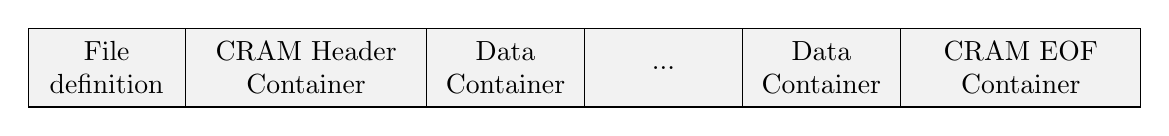
\begin{tikzpicture}[
  every node/.style={scale=1.0},
  boxes/.style={rectangle split,rectangle split parts=#1,draw,rectangle split horizontal,text width=5em,align=center,minimum height=1cm,fill=black!5,on grid},
  notes/.style={text width=20em,align=center,minimum height=1cm,on grid},
]
\node (file) [boxes=6] {
\nodepart{one}File definition
\nodepart[text width=8em]{two}CRAM Header Container
\nodepart{three}Data Container
\nodepart{four}...
\nodepart{five}Data Container
\nodepart[text width=8em]{six}CRAM EOF Container
};
\end{tikzpicture}

Figure 1: A CRAM file consists of a file definition, followed by a header container, then other containers.
\end{center}

Containers are just a Container Header Structure followed by one or
more Blocks.  Blocks have different types (see
~\ref{subsec:block-content-types}) corresponding to their usage.
Note the block itself also consists of a defined structure followed by
the block contents data.

\begin{center}
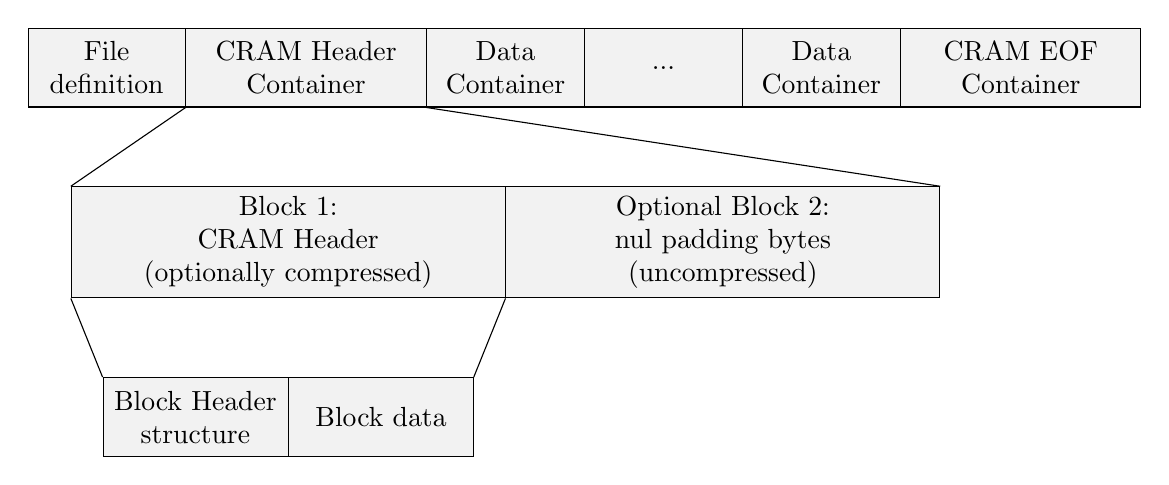
\begin{tikzpicture}[
  every node/.style={scale=1.0},
  boxes/.style={rectangle split,rectangle split parts=#1,draw,rectangle split horizontal,text width=5em,align=center,minimum height=1cm,fill=black!5,on grid},
  notes/.style={text width=20em,align=center,minimum height=1cm,on grid},
]
\node (file) [boxes=6] {
\nodepart{one}File definition
\nodepart[text width=8em]{two}CRAM Header Container
\nodepart{three}Data Container
\nodepart{four}...
\nodepart{five}Data Container
\nodepart[text width=8em]{six}CRAM EOF Container
};

\node (header) [boxes=2,below=1 of file.three south, text width=15em] {
\nodepart{one}Block 1:\break
CRAM Header\break
(optionally compressed)
\nodepart{two}Optional Block 2:\break
nul padding bytes\break
(uncompressed)
};
\draw (file.one split south) to (header.north west);
\draw (file.two split south) to (header.north east);

\node (blocks) [boxes=2,below=1 of header.one south,text width=6em] {
\nodepart{one}Block Header structure
\nodepart{two}Block data
};
\draw (header.south west) to (blocks.north west);
\draw (header.two split south) to (blocks.north east);
\end{tikzpicture}

Figure 2: The the first container holds the CRAM header text.
\end{center}

The first container, called the CRAM header container, is used to
store a textual header as described in the SAM specification (see the
section 7.1).  This is optionally followed by another uncompressed
block of nul padding bytes.  The purpose of this additional block is
to permit in-situ modification of the CRAM header without the
requirement to rewrite the entire file (instead needing just this
container to be rewritten, provided it can be padded to an identical
size).

\begin{center}
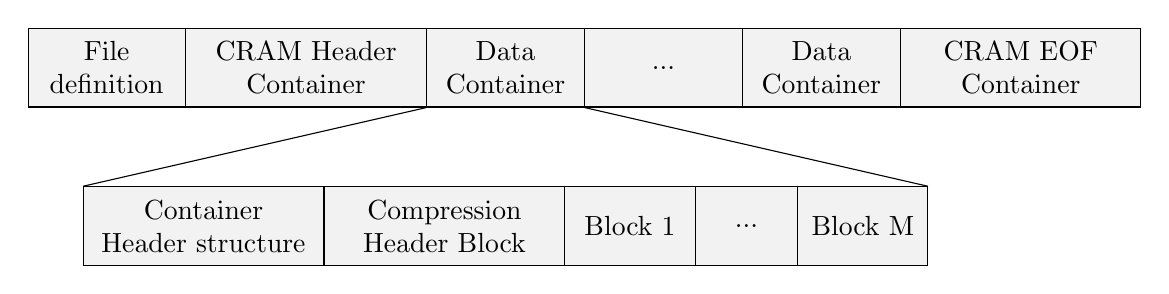
\begin{tikzpicture}[
  every node/.style={scale=1.0},
  boxes/.style={rectangle split,rectangle split parts=#1,draw,rectangle split horizontal,text width=5em,align=center,minimum height=1cm,fill=black!5,on grid},
  notes/.style={text width=20em,align=center,minimum height=1cm,on grid},
]
\node (file) [boxes=6] {
\nodepart{one}File definition
\nodepart[text width=8em]{two}CRAM Header Container
\nodepart{three}Data Container
\nodepart{four}...
\nodepart{five}Data Container
\nodepart[text width=8em]{six}CRAM EOF Container
};

\node (container) [boxes=5,below=1 of file.three south,text width=8em] {
\nodepart{one}Container Header structure
\nodepart{two}Compression Header Block
\nodepart[text width=4em]{three}Block 1
\nodepart[text width=3em]{four}...
\nodepart[text width=4em]{five}Block M
};
\draw (file.two split south) to (container.north west);
\draw (file.three split south) to (container.north east);
\end{tikzpicture}

Figure 3: Containers as a series of blocks
\end{center}

The Data Containers hold the sequence records themselves.
These start with a Compression Header block which holds meta-data
describing how and where the Data Series are encoded within this
container.

\begin{center}
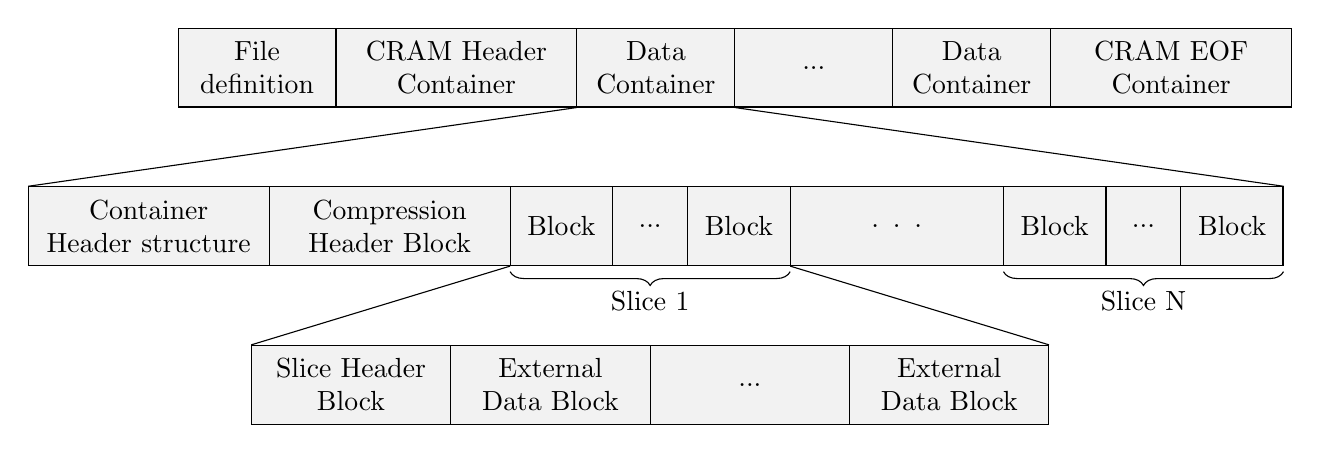
\begin{tikzpicture}[
  every node/.style={scale=1.0},
  boxes/.style={rectangle split,rectangle split parts=#1,draw,rectangle split horizontal,text width=5em,align=center,minimum height=1cm,fill=black!5,on grid},
  notes/.style={text width=20em,align=center,minimum height=1cm,on grid},
]
\node (file) [boxes=6] {
\nodepart{one}File definition
\nodepart[text width=8em]{two}CRAM Header Container
\nodepart{three}Data Container
\nodepart{four}...
\nodepart{five}Data Container
\nodepart[text width=8em]{six}CRAM EOF Container
};

\node (container) [boxes=9,below=1 of file.three south,text width=8em] {
\nodepart{one}Container Header structure
\nodepart{two}Compression Header Block
\nodepart[text width=3em]{three}Block
\nodepart[text width=2em]{four}...
\nodepart[text width=3em]{five}Block
\nodepart[text width=7em]{six}. . .
\nodepart[text width=3em]{seven}Block
\nodepart[text width=2em]{eight}...
\nodepart[text width=3em]{nine}Block
};
\draw (file.two split south) to (container.north west);
\draw (file.three split south) to (container.north east);

\draw[decoration={brace,mirror,amplitude=5pt,raise=2pt},decorate]
  (container.two split south) to (container.five split south);
\node [below=0.2 of container.four south] {Slice 1};

\draw[decoration={brace,mirror,amplitude=5pt,raise=2pt},decorate]
  (container.six split south) to (container.south east);
\node [below=0.2 of container.eight south] {Slice N};

\node (slice) [boxes=4,below=1 of container.four south, text width=6.5em] {
\nodepart{one}Slice Header Block
\nodepart{two}External Data Block
\nodepart{three}...
\nodepart{four}External Data Block
};
\draw (container.two split south) to (slice.north west);
\draw (container.five split south) to (slice.north east);
\end{tikzpicture}

Figure 4: Slices formed from a series of concatenated blocks
\end{center}

The blocks after the compression header are organised logically into slices. One 
slice may contain, for example, a contiguous region of alignment data. Slices begin 
with a slice header block and are followed by one or more data blocks.
It is these data blocks which hold the primary bulk of CRAM data, the
Data Series.

Note many CRAM files will just use one slice per contaner as this is
the default output format of several major implementations.

\subsection{File definition}

Each CRAM file starts with a fixed length (26 bytes) definition with the following 
fields:

\begin{tabular}{|l|l|l|}
\hline
\textbf{Data type} & \textbf{Name} & \textbf{Value}\tabularnewline
\hline
byte[4] & format magic number & CRAM (0x43 0x52 0x41 0x4d)\tabularnewline
\hline
byte & major format number & 3 (0x3)\tabularnewline
\hline
byte & minor format number & 1 (0x1)\tabularnewline
\hline
byte[20] & file id & CRAM file identifier (e.g. file name or SHA1 checksum)\tabularnewline
\hline
\end{tabular}

Valid CRAM \textit{major}.\textit{minor} version numbers are as follows:

\begin{itemize}
\item[\textit{1.0}]
The original public CRAM release.

\item[\textit{2.0}]
The first CRAM release implemented in both Java and C; tidied up
implementation vs specification differences in \textit{1.0}.

\item[\textit{2.1}]
Gained end of file markers; compatible with \textit{2.0}.

\item[\textit{3.0}]
Additional compression methods; header and data checksums;
improvements for unsorted data.

\item[\textit{3.1}]
Additional block compression codecs only.

\item[\textit{4.0}]
This specification.  Revised variable sized integers, MD/NM/RG tag
locators, and deduplication of read names.  Removed some encodings.
See \ref{sec:cram4changes} for a more detailed list of changes.
\end {itemize}

CRAM 3.0 and 3.1 differ only in the list of compression
methods available, so tools that output CRAM 3 without using any 3.1
codecs should write the header to indicate 3.0 in order to permit
maximum compatibility.

\subsection{Container header structure}

The file definition is followed by one or more containers with the following header 
structure where the container content is stored in the `blocks' field:

\begin{tabular}{|l|>{\raggedright}p{120pt}|>{\raggedright}p{260pt}|}
\hline
\textbf{Data type} & \textbf{Name} & \textbf{Value}
\tabularnewline
\hline
uint7 & length & the sum of the lengths of all blocks in this container (headers and data);
equal to the total byte length of the container minus the byte length of this header structure\tabularnewline
\hline
int7 & reference sequence id & reference sequence identifier  or\linebreak{}
-1 for unmapped reads\linebreak{}
-2 for multiple reference sequences.\linebreak{}
All slices in this container must have a reference sequence id matching this value.\tabularnewline
\hline
uint7 & starting position on the reference & the alignment start position or\linebreak{}
0 if the container is multiple-reference
or contains unmapped unplaced reads\tabularnewline
\hline
uint7 & alignment span & the length of the alignment or\linebreak{}
0 if the container is multiple-reference
or contains unmapped unplaced reads\tabularnewline
\hline
uint7 & number of records & number of records in the container\tabularnewline
\hline
uint7 & record counter & 1-based sequential index of records in the file/stream.\tabularnewline
\hline
uint7 & bases & number of read bases\tabularnewline
\hline
uint7 & number of blocks & the total number of blocks in this container\tabularnewline
\hline
array<uint7> & landmarks & the locations of slices in this container as byte offsets from the end of 
this container header, used for random access indexing.
The landmark count must equal the slice count.\linebreak{}
Since the block before the first slice is the compression header,
landmarks[0] is equal to the byte length of the compression header.\tabularnewline
\hline
uint32 & crc32 & CRC32 hash of the all the preceding bytes in the container.\tabularnewline
\hline
byte[ ] & blocks & The blocks contained within the container.\tabularnewline
\hline
\end{tabular}

\subsubsection*{CRC32}
This is a cyclic redundancy checksum 32-bit long with the polynomial 0x04C11DB7. Please refer to \href{http://www.itu.int/rec/recommendation.asp?type=folders&lang=e&parent=T-REC-V.42}{ITU-T V.42} for more details. The value of the CRC32 hash function is written as an integer.


\subsection{Block structure}
\label{sec:block-struct}

Containers consist of one or more blocks. Block compression is applied independently 
and in addition to any encodings used to compress data within the block. The block 
have the following header structure with the data stored in the `block data' field:

\begin{tabular}{|l|>{\raggedright}p{120pt}|>{\raggedright}p{260pt}|}
\hline
\textbf{Data type} & \textbf{Name} & \textbf{Value}
\tabularnewline
\hline
byte & method & the block compression method (and first CRAM version): \linebreak{}
0: raw (none)*\linebreak{}
1: gzip\linebreak{}
2: bzip2 (v2.0)\linebreak{}
3: lzma (v3.0)\linebreak{}
4: rans4x8 (v3.0)\linebreak{}
5: rans4x16 (v3.1)\linebreak{}
6: adaptive arithmetic coder (v3.1)\linebreak{}
7: fqzcomp (v3.1)\linebreak{}
8: name tokeniser (v3.1)
\tabularnewline
\hline
byte & block content type id & the block content type identifier\tabularnewline
\hline
uint7 & block content id & the block content identifier used to associate
data blocks with data series\tabularnewline
\hline
uint7 & size in bytes* & size of the block data after applying block compression\tabularnewline
\hline
uint7 & raw size in bytes* & size of the block data before applying block compression\tabularnewline
\hline
byte[ ] & block data & the data stored in the block\tabularnewline
\hline
uint32 & CRC32 & CRC32 hash value for all preceding bytes in the block\tabularnewline
\hline
\end{tabular}

* Note on raw method: both compressed and raw sizes must be set to the same value.

\subsubsection*{Block content types}
\label{subsec:block-content-types}

CRAM has the following block content types:

\begin{threeparttable}[t]
\begin{tabular}{|>{\raggedright}p{143pt}|>{\raggedright}p{45pt}|>{\raggedright}p{116pt}|>{\raggedright}p{114pt}|}
\hline
\textbf{Block content type} & \textbf{Block content type id} & \textbf{Name} & \textbf{Contents}\tabularnewline
\hline
FILE\_HEADER & 0 & CRAM header block & CRAM header\tabularnewline
\hline
COMPRESSION\_HEADER & 1 & Compression header block & See specific section\tabularnewline
\hline
SLICE\_HEADER & 2 & Slice header block & See specific section\tabularnewline
\hline
 & 3 &  & reserved\tabularnewline
\hline
EXTERNAL\_DATA & 4 & data block & data produced by encodings\tabularnewline
\hline
\end{tabular}
\end{threeparttable}

\subsubsection*{Block content id}

Block content id is used to distinguish between data blocks in the same slice. 
Each encoding has an id parameter which must be one of the block
content ids. For data blocks the content id is a positive integer. For all
other blocks content id should be 0. Consequently, all data encodings must 
not use content id less than 1. 

\subsection{CRAM header container}

The first container in a CRAM file contains a textual header in a single block, optionally
gzip compressed. This text header currently matches the SAM header specification. Only
gzip is allowed as compression method for this block. The CRAM header container does not
include a compression header block.

The following constraints apply to the SAM header: 

\begin{itemize}
\item The SQ:MD5 checksum is required unless the reference sequence has been embedded 
into the file.
\end{itemize}

It is recommended to reserve 50\% more space in the CRAM header container than
is required for the SAM header text by optionally padding the container with a second
raw block consisting of all zeroes. This can be used to subsequently expand the header
container in place, such as when updating @SQ records, while preserving the absolute
offsets of all subsequent containers.

\subsection{Compression header block}
\label{subsec:compression-header}

The compression header block consists of 3 parts: preservation map, data series 
encoding map and tag encoding map.  See below for the data format of a map.

These are meta-data on what is stored in the following slices, how it is encoded, and in which blocks the raw byte streams from these encodings reside.

\begin{tabular}{|l|>{\raggedright}p{120pt}|>{\raggedright}p{260pt}|}
\hline
\textbf{Data type} & \textbf{Name} & \textbf{Value}
\tabularnewline
\hline
map & preservation map & meta-data about types of data stored and dictionaries \tabularnewline
\hline
map & data series encoding map & meta-data for how data series are encoded \tabularnewline
\hline
map & tag encoding map & meta-data for how tags are encoded \tabularnewline
\hline
\end{tabular}

\subsubsection{Map structure}

% FIXME: is this better defined as a sub-structure in the relevant section itself?
% Possibly...
A \textit{Map} is a collection of keys and associated values.

Both the size in bytes and the number of keys are written as integer (uint7). Keys 
and values are written according to their data types and are specific to each map.
Keys have a fixed size for all items in a map, but this size is not
the same for all map types.  The order of keys is not defined.  Values
are stored immediately after their key in a key-defined format.  Some
keys will have simple boolean values, some are fixed size, while
others have a more complex sub-structures.

The example below is for a two byte key map.

\begin{tabular}{|l|>{\raggedright}p{120pt}|>{\raggedright}p{260pt}|}
\hline
\textbf{Data type} & \textbf{Name} & \textbf{Value}
\tabularnewline
\hline
uint7 & size & the remaining size in bytes of this map structure\tabularnewline
\hline
uint7 & num\_keys & the number of key-value pairs in this map\tabularnewline
\hline
byte[2] & key & first key\tabularnewline
\hline
byte[] & value & first value, with a key-specific size (see below).\tabularnewline
\hline
... & ... & \textit{repeated num\_keys time}\tabularnewline
\hline
\end{tabular}


\subsubsection{Preservation map}

The preservation map contains information about which data was preserved in the 
CRAM file. It is stored as a map with byte[2] keys:

\begin{tabular}{|l|l|>{\raggedright}p{100pt}|>{\raggedright}p{220pt}|}
\hline
\textbf{Key} & \textbf{Value data type} & \textbf{Name} & \textbf{Value}\tabularnewline
\hline
RN & bool & read names included & true if read names are preserved for all reads\tabularnewline
\hline
AP & bool & AP data series delta & true if AP data series is delta, false otherwise\tabularnewline
\hline
RR & bool & reference required & true if reference sequence is required to restore 
the data completely\tabularnewline
\hline
SM & byte[5] & substitution matrix & substitution matrix\tabularnewline
\hline
TD & array\texttt{<}byte\texttt{<>} & tag ids dictionary & a list of lists of tag ids, see tag encoding 
section\tabularnewline
\hline
QO & bool & qual orientation & true if quality values are in the same orientation as sequence.  If false quality values are recorded in the orientation as produced by the sequencing instrument, which may also still match sequence orientation.\tabularnewline
\hline
\end{tabular}

The boolean values are optional, defaulting to true when absent, although it is recommended to explicitly set them.  SM and TD are mandatory.

\subsubsection{Encoding structure}

The data series encoding map utilises another custom data type, \textit{encoding\texttt{<}type\texttt{>}}.
This is used to describe the data encapsulation format for a specific data series; how and where the values are stored.  This could be
the definition of a constant, a series of data transformations, or the
block content id for a data block.  Some encodings may be nested,
such as \texttt{BYTE\_ARRAY\_LEN} which defines one sub-encoding for the
length and another for the bytes.

Encoding notation is defined as the keyword `encoding' followed by its data type in angular brackets, for example `encoding\texttt{<}byte\texttt{>}' stands for an encoding that operates on a data series of data type `byte'.
Note there are distinct encodings dealing with signed and unsigned
data in addition to offsets applies to each, so for integer data the
data series use `encoding\texttt{<}int\texttt{>}` and let the specific
encoding and meta-data handle the sign as appropriate.

The \textit{encoding} format consists of an encoding type and type specific meta-data stored as an array (dimension followed by the array elements).

\begin{tabular}{|l|>{\raggedright}p{120pt}|>{\raggedright}p{260pt}|}
\hline
\textbf{Data type} & \textbf{Name} & \textbf{Value}
\tabularnewline
\hline
uint7 & encoding\_ID & encoding type identifier\tabularnewline
\hline
array\texttt{<}byte\texttt{>} & encoding\_meta & type specific meta-data for this encoding, serialised as a byte stream\tabularnewline
\hline
\end{tabular}

\vskip 10pt

Note unlike the fields in structures, data series types here do not
distinguish signed integer (sint) vs unsigned integer (uint) as this
distinction is handled by the encoding itself.  This is different to
CRAM 3.0 and earlier where the sign and size of the data series types
was written into the specification, rather than stored as meta-data in
the CRAM file.

For example, the alignment position (\textbf{AP}) data series has a value data type of \textit{encoding<int>}.
Typically on a position sorted file this is delta encoded and all
values are positive, so a suitable encoding is VARINT\_UNSIGNED.  If
the slice contains data aligned against multiple reference sequences
then this may contain some negative deltas in which case
VARINT\_SIGNED could be appropriate.

A list of data types along with their possible encodings is listed
below.

\begin{tabular}{llll}
\textbf{ID}  & \textbf{Encoding} & \textbf{Data Type} & \textbf{Description}\\
\hline
\\
0  & NULL             & \textit{N/A} & Data series not present\\
\\
1  & BYTE (EXTERNAL)  & byte   & An unsigned single byte (8 bits)  \\
\\
4  & BYTE\_ARRAY\_LEN & byte[] & Zero or more items with unspecified length\\
5  & BYTE\_ARRAY\_STOP& byte[] & Zero or more items with unspecified length\\
\\
41 & VARINT\_UNSIGNED & int    & A variable length integer (VLQ $x >= 0$)\\
42 & VARINT\_SIGNED   & int    & A variable length integer (VLQ, may be negative)\\
\\
43 & CONST\_BYTE      & byte   & A fixed byte value\\
44 & CONST\_INT       & int    & A fixed integer value (VLQ, signed)\\
\end{tabular}

\vskip 10pt

See section~\ref{sec:encodings} for more detailed descriptions of all
the above coding algorithms and their parameters.  Note the encoding
ID values here have been chosen to not clash with CRAM 3.0 and earlier
with the exception of the BYTE\_ARRAY\_LEN and BYTE\_ARRAY\_STOP
encodings which have not changed and BYTE which is identical and
synonymous with EXTERNAL in the CRAM 3.0 specification.

\subsubsection{Data series encoding map}

Writing to and reading from data blocks is organised through CRAM
records. A CRAM record is analogous to a single line in a SAM file.

The records are organised into slices and then each slice is
rearranged in a columnar fashion into data series.  For example
collect 10,000 SAM records and then the first column, query name
(QNAME), becomes one CRAM data series (RN), the next column (FLAG)
becomes CRAM data series (BF), and so on.  Note some SAM columns, such
as CIGAR, may map to many CRAM data series.

Each data series is associated with an encoding. An encoding may have
a block content id which is used to identify the block where the data
series is stored. Please note that data blocks can have multiple
data series associated with them; in this case the values from these
data series will be interleaved and must be decoded in the correct order.

\begin{center}
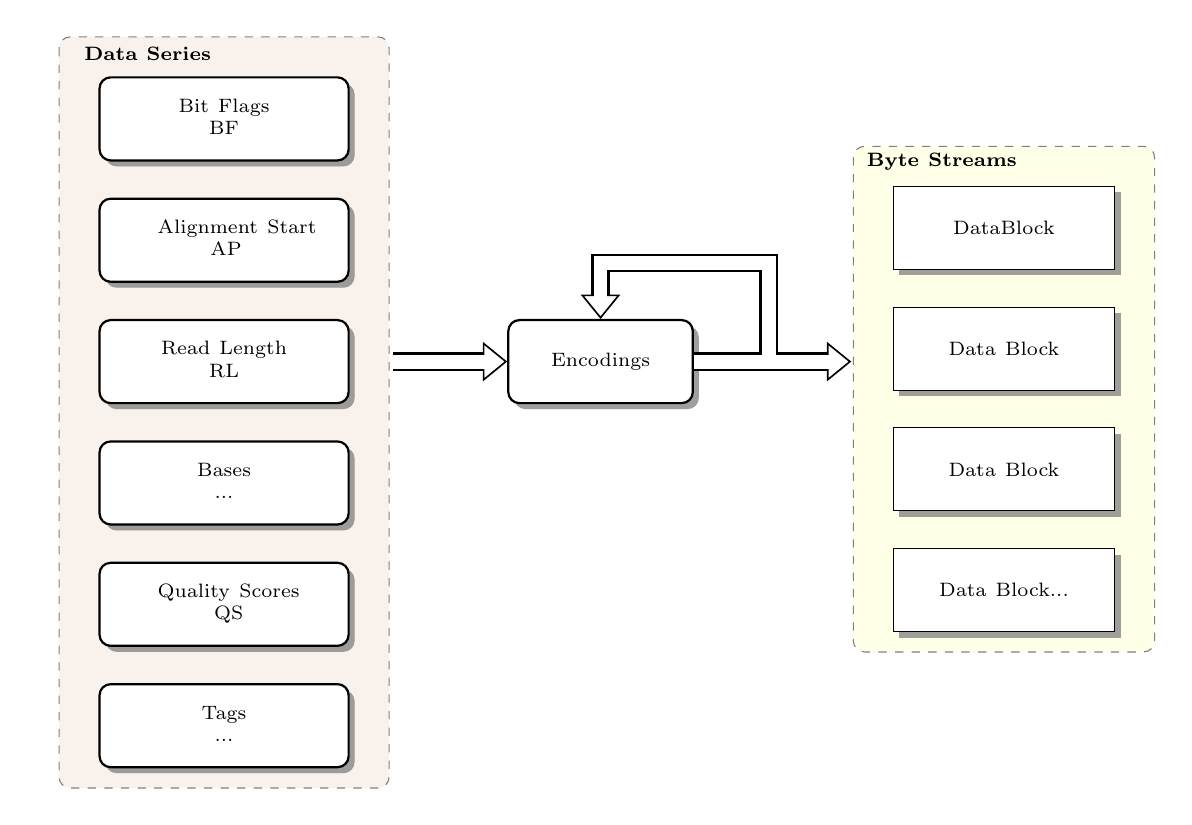
\begin{tikzpicture}[thick]

\usetikzlibrary{shapes, shadows, positioning, arrows,  decorations.markings, arrows.meta}

\pgfdeclarelayer{background}
\pgfsetlayers{background,main}

\tikzstyle{dsbox} = [blockbox, text width=6em, minimum width=9em, minimum height=3em, rounded corners, drop shadow]
\tikzstyle{blockbox}=[draw, fill=white, text width=4.0em, text centered, minimum height=1.0em, drop shadow]
\tikzstyle{encodedblock} = [blockbox, text width=6em, minimum width=8em, minimum height=3em, drop shadow]
\tikzstyle{encodings} = [dsbox, minimum width=6em, thick]

\tikzstyle{texto} = [above, text width=8em, text centered]

\tikzstyle{vecArrow} = [thick, decoration={markings,mark=at position
   1 with {\arrow[semithick]{Triangle[open, length=3.1mm, width=5mm]}}},
   double distance=5pt, shorten >= 8.5pt,
   preaction = {decorate},
   postaction = {draw,line width=5pt, white,shorten >= 8pt}]
\tikzstyle{innerWhite} = [semithick, white,line width=5pt, shorten >= 8pt]

\newcommand{\cramRecord}[6]{%
\begin{pgfonlayer}{background}
    \path (#1.west |- #1.north) + (-0.5, 0.5) node (a1) {};
    \path (#1.east |- #6.south) + (+0.5,-0.25) node (a2) {};
    \path[fill=brown!10,rounded corners, draw=black!50, dashed]
      (a1) rectangle (a2);
    \path (a1.east |- a1.south) + (1.0,-0.3) node[texto]
    {\scriptsize\textbf{Data Series}};
\end{pgfonlayer}}

\newcommand{\dsbox}[2]{node (p#1) [dsbox]
{\scriptsize{#2}}}
\newcommand{\encodedblock}[2]{node (p#1) [encodedblock]
	{\scriptsize{#2}}}
\newcommand{\encodedblocklarge}[2]{node (p#1) [encodedblocklarge]
   {\scriptsize{#2}}}

\path +(-2.5,-1.5) \dsbox{1}{\begin{tabular}{c} Bit Flags \\ BF \end{tabular}};
\path (p1.south)+(0.0,-1.0) \dsbox{2}{\begin{tabular}{c} Alignment Start\\ AP\quad\quad \end{tabular}};
\path (p2.south)+(0.0,-1.0) \dsbox{3}{\begin{tabular}{c} Read Length \\ RL \end{tabular}};
\path (p3.south)+(0.0,-1.0) \dsbox{4}{\begin{tabular}{c} Bases \\ ... \end{tabular}};
\path (p4.south)+(0.0,-1.0) \dsbox{5}{\begin{tabular}{c} Quality Scores \\ QS \end{tabular}};
\path (p5.south)+(0.0,-1.0) \dsbox{6}{\begin{tabular}{c} Tags \\ ... \end{tabular}};

\cramRecord{p1}{p2}{p3}{p4}{p5}{p6}

\newcommand{\blockStreams}[4]{%
\begin{pgfonlayer}{background}
    \path (#1.west |- #1.north)+(-0.5, 0.5) node (a3) {};
    \path (#4.east |- #4.south)+(+0.5, -0.25) node (a4) {};
    \path[fill=yellow!10, rounded corners, draw=black!50, dashed]
      (a3) rectangle (a4);
    \path (a3.east |- a3.south)+(1.0,-0.3) node[texto]{\scriptsize\textbf{Byte Streams}};
\end{pgfonlayer}}

\path (a1.south) + (12.0, -2.3) \encodedblock {7} {DataBlock};
\path (p7.south) + (0.0, -1.0)  \encodedblock {8} {Data Block};
\path (p8.south) + (0.0, -1.0)  \encodedblock {9} {Data Block}; 
\path (p9.south) + (0.0, -1.0)  \encodedblock {10}{Data Block...};

\blockStreams {p7} {p8} {p9} {p10}

\node (encodings) [encodings, right = 2 of p3] {\scriptsize Encodings};
\node (enc_e1) [right=0.7 of encodings] {};
\node (enc_e2) [right=1.05 of enc_e1] {};
\node (enc_n)  [above=1 of encodings.center] {};
\draw[vecArrow] (p3.east) + (0.55, 0) to (encodings.west);
\draw[vecArrow] (encodings.east) to (enc_e2.west);
\draw[vecArrow] (enc_e1.east) |- (enc_n.north) to (encodings.north);
\draw[innerWhite] (encodings.east) to (enc_e2.west);

\end{tikzpicture}

Figure 5: The relationship between Data Series, Possibly nested Encodings, and Data Blocks.

\end{center}

The picture shows how a CRAM record (on the left) is distributed to
multiple Data Blocks via a series of encodings.  Note the mapping from
Data Series to Blocks may be many to many, with the possibility of
multiple Data Series writing to the same Block and with a single
encoding such as BYTE\_ARRAY\_LEN potentially writing to two Blocks.


Each data series has an encoding. These encodings are stored in a map with byte[2] 
keys and are decoded in approximately this order\footnote{The precise order is defined in section~\ref{sec:record}.}:

\begin{threeparttable}[t]
\begin{tabular}{|l|l|>{\raggedright}p{100pt}|>{\raggedright}p{220pt}|}
\hline
\textbf{Key} & \textbf{Value data type} & \textbf{Name} & \textbf{Value}\tabularnewline
\hline
BF & encoding\texttt{<}int\texttt{>} & BAM bit flags & see separate section\tabularnewline
\hline
CF & encoding\texttt{<}int\texttt{>} & CRAM bit flags & see specific section\tabularnewline
\hline
RI & encoding\texttt{<}int\texttt{>} & reference id & record reference id from
the SAM file header\tabularnewline
\hline
RL & encoding\texttt{<}int\texttt{>} & read lengths & read lengths\tabularnewline
\hline
AP & encoding\texttt{<}int\texttt{>} & in-seq positions & if \textbf{AP-Delta} = true: 0-based alignment start
delta from the AP value in the previous record.
Note this delta may be negative, for example when switching references in a multi-reference slice.
When the record is the first in the slice, the previous position used is the slice alignment-start field (hence the first delta should be zero for single-reference slices, or the AP value itself for multi-reference slices).  \linebreak{}
if \textbf{AP-Delta} = false: encodes the alignment start position directly\tabularnewline
\hline
RG & encoding\texttt{<}int\texttt{>} & read groups & read groups. Special value 
`-1' stands for no group.\tabularnewline
\hline
RN\tnote{a} & encoding\texttt{<}byte[ ]\texttt{>} & read names & read names\tabularnewline
\hline
MF & encoding\texttt{<}int\texttt{>} & next mate bit flags & see specific section\tabularnewline
\hline
NS & encoding\texttt{<}int\texttt{>} & next fragment reference sequence id & reference 
sequence ids for the next fragment \tabularnewline
\hline
NP & encoding\texttt{<}int\texttt{>} & next mate alignment start & alignment positions 
for the next fragment\tabularnewline
\hline
TS & encoding\texttt{<}int\texttt{>} & template size & template sizes\tabularnewline
\hline
NF & encoding\texttt{<}int\texttt{>} & distance to next fragment & number of records
to the next fragment\tnote{b}\tabularnewline
\hline
TL\tnote{c} & encoding\texttt{<}int\texttt{>} & tag ids  & list of tag ids, see tag encoding
section\tabularnewline
\hline
FN & encoding\texttt{<}int\texttt{>} & number of read features & number of read
features in each record\tabularnewline
\hline
FC & encoding\texttt{<}byte\texttt{>} & read features codes & see separate section\tabularnewline
\hline
FP & encoding\texttt{<}int\texttt{>} & in-read positions & positions of the read
features; a positive delta to the last position (starting with zero)\tabularnewline
\hline
DL & encoding\texttt{<}int\texttt{>} & deletion lengths & base-pair deletion lengths\tabularnewline
\hline
BB & encoding\texttt{<}byte[ ]\texttt{>} & stretches of bases & bases\tabularnewline
\hline
QQ & encoding\texttt{<}byte[ ]\texttt{>} & stretches of quality scores & quality scores\tabularnewline
\hline
BS & encoding\texttt{<}byte\texttt{>} & base substitution codes & base substitution
codes\tabularnewline
\hline
IN & encoding\texttt{<}byte[ ]\texttt{>} & insertion & inserted bases\tabularnewline
\hline
RS & encoding\texttt{<}int\texttt{>} & reference skip length & number of skipped 
bases for the `N' read feature\tabularnewline
\hline
PD & encoding\texttt{<}int\texttt{>} & padding & number of padded bases\tabularnewline
\hline
HC & encoding\texttt{<}int\texttt{>} & hard clip & number of hard clipped bases\tabularnewline
\hline
SC & encoding\texttt{<}byte[ ]\texttt{>} & soft clip & soft clipped bases\tabularnewline
\hline
MQ & encoding\texttt{<}int\texttt{>} & mapping qualities & mapping quality scores\tabularnewline
\hline
BA & encoding\texttt{<}byte\texttt{>} & bases & bases\tabularnewline
\hline
QS & encoding\texttt{<}byte\texttt{>} & quality scores & quality scores\tabularnewline
\hline
\end{tabular}

\begin{tablenotes}
\item[a] Note RN this is decoded after MF if the record is detached from the mate and we are attempting to auto-generate read names.
\item[b] The count is reset for each slice so NF can only refer to a record later within this slice.
\item[c] Decode of TL is followed by decoding the tag values themselves, in order of appearance in the tag dictionary.
\end{tablenotes}
\end{threeparttable}

\subsubsection{Tag encoding map}
\label{subsubsec:tags}

The tag dictionary (TD) describes the unique combinations of tag id / type that occur on each alignment record.
For example if we search the id / types present in each record and find only two combinations -- X1:i BC:Z SA:Z: and X1:i: BC:Z -- then we have two dictionary entries in the TD map.

Let $L_{i}=\{T_{i0}, T_{i1}, \ldots, T_{ix}\}$ be a list of all tag ids for a record $R_{i}$, where $i$ is the sequential record index and $T_{ij}$ denotes $j$-th tag id in the record.
The list of unique $L_{i}$ is stored as the TD value in the preservation map.
Maintaining the order is not a requirement for encoders (hence ``combinations''), but it is permissible and thus different permutations, each encoded with their own elements in TD, should be supported by the decoder.
Each $L_{i}$ element in TD is assigned a sequential integer number starting with 0.
These integer numbers are referred to by the TL data series.
Using TD, an integer from the TL data series can be mapped back into a list of tag ids.
Thus per alignment record we only need to store tag values and not their ids and types.

The TD is written as a byte array consisting of $L_{i}$ values separated with \textbackslash{}0.
Each $L_{i}$ value is written as a concatenation of 3 byte $T_{ij}$ elements: tag id followed by BAM tag type code (one of A, c, C, s, S, i, I, f, F, Z, H or B, as described in the SAM specification) or \texttt{*}.
Type code \texttt{*} is used as a placeholder to mark the presence and location of the MD, NM or RG tags.

For example the TD for tag lists X1:i BC:Z SA:Z and X1:i MD:Z NM:i BC:Z may be encoded as\\
X1CBCZSAZ\textbackslash{}0X1CMD*NM*BCZ\textbackslash{}0, with X1C indicating a 1 byte unsigned value for tag X1 and an assumption that all MD and NM tags present can be auto-generated.

\subsubsection*{Tag values}

The encodings used for different tags are stored in a map.
The key is 3 bytes formed from the BAM tag id and type code, matching the TD dictionary described above.
Unlike the Data Series Encoding Map, the key is stored in the map as a uint7 encoded integer, constructed using $(char1<<16) + (char2<<8) + type$.
For example, the 3-byte representation of OQ:Z is \{0x4F, 0x51, 0x5A\} and these bytes are intepreted as the integer key 0x004F515A, leading to an uint7 byte stream \{0x82, 0xbd, 0xa2, 0x59\}.

\begin{tabular}{|l|l|l|>{\raggedright}p{160pt}|}
\hline
\textbf{Key} & \textbf{Value data type} & \textbf{Name} & \textbf{Value}
\tabularnewline
\hline
TAG ID 1:TAG TYPE 1 & encoding\texttt{<}byte[ ]\texttt{>} & read tag 1 & tag values
(names and types are available in the data series code)\tabularnewline
\hline
... &  & ... & ...\tabularnewline
\hline
TAG ID N:TAG TYPE N & encoding\texttt{<}byte[ ]\texttt{>} & read tag N & ...\tabularnewline
\hline
\end{tabular}

Note that tag values are encoded as array of bytes. The routines to convert tag 
values into byte array and back are the same as in BAM with the exception of value 
type being captured in the tag key rather in the value.
Hence consuming 1 byte for types `C' and `c', 2 bytes for types `S' and `s', 4 bytes for types `I', `i' and `f', and a variable number of bytes for types `H', `Z' and `B'.

\subsection{Slice header block}

The slice header block is never compressed (block method=raw). For reference mapped 
reads the slice header also defines the reference sequence context of the data 
blocks associated with the slice. Mapped reads can be stored along with
\textbf{placed unmapped}\footnote{Unmapped reads can be \textit{placed} or \textit{unplaced}.
A read that is unmapped according to bit 0x4 of the BF (BAM bit flags)
data series, but has position and reference fields filled in, is
\textit{placed unmapped}.  In contrast, \textit{unplaced unmapped}
reads have have a reference sequence ID of -1 and alignment position of 0.}
reads on the same reference within the same slice.

Slices with the Multiple Reference flag (-2) set as the sequence ID in the header may contain reads
mapped to multiple external references, including unmapped\footnotemark[\value{footnote}] reads (placed on these references or unplaced),
but multiple embedded references cannot be combined in this way.  When multiple references are
used, the RI data series will be used to determine the reference sequence ID for each record.  This
data series is not present when only a single reference is used within a slice.

The Unmapped (-1) sequence ID in the header is for slices containing only unplaced
unmapped\footnotemark[\value{footnote}] reads.

A slice containing data that does not use the external reference in
any sequence may set the reference MD5 sum to zero.  This can happen
because the data is unmapped or the sequence has been stored verbatim
instead of via reference-differencing.  This latter scenario is
recommended for unsorted or non-coordinate-sorted data.

The slice header block contains the following fields.

\begin{tabular}{|l|l|>{\raggedright}p{200pt}|}
\hline
\textbf{Data type} & \textbf{Name} & \textbf{Value}\tabularnewline
\hline
int7 & reference sequence id & reference sequence identifier or\linebreak{}
-1 for unmapped reads\linebreak{}
-2 for multiple reference sequences.\linebreak{}
This value must match that of its enclosing container.\tabularnewline
\hline
uint7 & alignment start & the alignment start position.\linebreak{}
0 if the slice is multiple-reference
or contains unmapped unplaced reads\tabularnewline
\hline
uint7 & alignment span & the length of the alignment.\linebreak{}
0 if the slice is multiple-reference
or contains unmapped unplaced reads\tabularnewline
\hline
uint7 & number of records & the number of records in the slice\tabularnewline
\hline
uint7 & record counter & 1-based sequential index of records in the file/stream\tabularnewline
\hline
uint7 & number of blocks & the number of blocks in the slice\tabularnewline
\hline
uint7[ ] & block content ids & block content ids of the blocks in the slice\tabularnewline
\hline
uint7 & embedded reference bases block content id & block content id for the embedded 
reference sequence bases or 0 for none\tabularnewline
\hline
byte[16] & reference md5 & MD5 checksum of the reference bases within the slice 
boundaries.  If this slice has reference sequence id of -1 (unmapped) or -2 (multi-ref)
the MD5 should be 16 bytes of \textbackslash{}0. For embedded references, the MD5
can either be all-zeros or the MD5 of the embedded sequence.\tabularnewline
\hline
byte[] & optional tags & a series of tag,type,value tuples encoded as
per BAM auxiliary fields.\tabularnewline
\hline
\end{tabular}

The optional tags are encoded in the same manner as BAM tags.  I.e. a
series of binary encoded tags concatenated together where each tag
consists of a 2 byte key (matching [A-Za-z][A-Za-z0-9]) followed by a
1 byte type ([AfZHcCsSiIB]) followed by a string of bytes in a format
defined by the type.

Tags starting in a capital letter are reserved while lowercase ones or
those starting with X, Y or Z are user definable.  Any tag not
understood by a decoder should be skipped over without producing an
error.

At present no tags are defined, but potential uses include additional
checksums and statistical information.

% Details omitted until we fully work through all the corner cases,
% such as seq/qual of *.
%
% Reserved tags are defined as follows:
% 
% \begin{tabular}{|l|l|>{\raggedright}p{325pt}|}
% \hline
% \textbf{Tag type} & \textbf{BAM format} & \textbf{Meaning}\tabularnewline
% \hline
% BD & i & Sum over all reads of the CRC32 hash of sequence base.  This
% may be used to validate round-trips in and out of CRAM.
% calls\tabularnewline
% \hline
% SD & i & Sum over all reads of the CRC32 hash of quality scores. (If
% the quality string is ``*'' in SAM then the hash is of the BAM encoded
% version - a string of bytes with value 255.)\tabularnewline
% \hline
% \end{tabular}


\subsection{End of file container}

A special container is used to mark the end of a file or stream. It is required in version 3 or later.
The idea is to provide an easy and a quick way to detect that a CRAM file or stream is complete.
The marker is an empty container with ref seq id set to -1 (unaligned) and alignment start set to 4542278 (which is ``EOF'' when seen in ASCII).

It is recommended that implementations of CRAM validate EOF by checking these values rather than direct comparison of byte values, as these checks will be valid for all versions of CRAM

\section{Record structure}
\label{sec:record}

CRAM record is based on the SAM record but has additional features allowing for 
more efficient data storage.  In contrast to BAM record CRAM records
are separated by type of data into a series of data blocks.  These
blocks can then use content type aware compression techniques.

As CRAM data series may be interleaved within the same blocks\footnote{Interleaving can sometimes provide better compression, however it also adds dependency between types of data meaning it is not possible to selectively decode one data series if it co-locates with another data series in the same block.} understanding the order in which CRAM data series must be decoded is vital.

The overall flowchart is below, with more detailed description in the subsequent sections.

\algnewcommand\algorithmicto{\text{ \textbf{to} }}

\subsection{CRAM record}

Both mapped and unmapped reads start with the following fields. Please note that 
the data series type refers to the logical data type and the data series name corresponds 
to the data series encoding map.

\begin{tabular}{|>{\raggedright}p{70pt}|>{\raggedright}p{75pt}|>{\raggedright}p{90pt}|>{\raggedright}p{171pt}|}
\hline
\textbf{Data series type} & \textbf{Data series name} & \textbf{Field} & \textbf{Description}\tabularnewline
\hline
uint & BF & BAM bit flags & see BAM bit flags below\tabularnewline
\hline
uint & CF & CRAM bit flags & see CRAM bit flags below\tabularnewline
\hline
- & - & Positional data & See section \ref{subsec:positions}\tabularnewline
\hline
- & - & Read names & See section \ref{subsec:names}\tabularnewline
\hline
- & - & Mate records & See section \ref{subsec:mate}\tabularnewline
\hline
- & - & Auxiliary tags & See section \ref{subsec:tags}\tabularnewline
\hline
- & - & Sequences & See sections \ref{subsec:mapped} and \ref{subsec:unmapped}\tabularnewline
\hline
\end{tabular}

\subsubsection*{BAM bit flags (BF data series)}

The following flags are duplicated from the SAM and BAM specification, with identical meaning.
Note however some of these flags can be derived during decode, so may be omitted in the CRAM file and the bits computed based on both reads of a pair-end library residing within the same slice.

\begin{threeparttable}[t]
\begin{tabular}{|l|l|l|}
\hline
\textbf{Bit flag} & \textbf{Comment} & \textbf{Description}\tabularnewline
\hline
0x1 &  & template having multiple segments in sequencing\tabularnewline
\hline
0x2 &  & each segment properly aligned according to the aligner\tabularnewline
\hline
0x4 &  & segment unmapped\tnote{a}\tabularnewline
\hline
0x8 & calculated\tnote{b}\ \ or stored in the mate's info & next segment in template unmapped\tabularnewline
\hline
0x10 &  & SEQ being reverse complemented\tabularnewline
\hline
0x20 & calculated\tnote{b}\ \ or stored in the mate's info & SEQ of the next segment in the
template being reverse complemented\tabularnewline
\hline
0x40 &  & the first segment in the template\tnote{c}\tabularnewline
\hline
0x80 &  & the last segment in the template\tnote{c}\tabularnewline
\hline
0x100 &  & secondary alignment\tabularnewline
\hline
0x200 &  & not passing quality controls\tabularnewline
\hline
0x400 &  & PCT or optical duplicate\tabularnewline
\hline
0x800 &  & Supplementary alignment\tabularnewline
\hline
\end{tabular}
\begin{tablenotes}
\item[a] Bit 0x4 is the only reliable place to tell whether the read is unmapped.  If 0x4 is set, no assumptions may be made about bits 0x2, 0x100 and 0x800.
\item[b] For segments within the same slice.
\item[c] Bits 0x40 and 0x80 reflect the read ordering within each template inherent in the sequencing technology used, which may be independent from the actual mapping orientation.
If 0x40 and 0x80 are both set, the read is part of a linear template (one where the template sequence is expected to be in a linear order), but it is neither the first nor the last read.
If both 0x40 and 0x80 are unset, the index of the read in the template is unknown.
This may happen for a non-linear template (such as one constructed by stitching together other templates) or when this information is lost during data processing.
\end{tablenotes}
\end{threeparttable}

\subsubsection*{CRAM bit flags (CF data series)}

The CRAM bit flags (also known as compression bit flags) expressed as an integer represent the CF data series. 
The following compression flags are defined for each CRAM read record:

\begin{tabular}{|>{\raggedright}p{39pt}|>{\raggedright}p{150pt}|>{\raggedright}p{242pt}|}
\hline
\textbf{Bit flag} & \textbf{Name} & \textbf{Description}\tabularnewline
\hline
0x1 & quality scores stored as array & quality scores can be stored as read features
or as an array similar to read bases.\tabularnewline
\hline
0x2 & detached & mate information is stored verbatim (e.g. because the pair spans multiple slices or the fields differ to the CRAM computed method)\tabularnewline
\hline
0x4 & has mate downstream & tells if the next segment should be expected further
in the stream\tabularnewline
\hline
0x8 & decode sequence as ``*'' & informs the decoder that the sequence
is unknown and that any encoded reference differences are present only to
recreate the CIGAR string.\tabularnewline
\hline
0x10 & explicit template size & decode from the template size (TS) data series even for record in an attached pair.\tabularnewline
\hline
\end{tabular}


The following pseudocode describes the general process of decoding an entire CRAM record.
The sequence data itself is in one of two encoding formats depending on whether the record is aligned (mapped).

\subsubsection*{Decode pseudocode}
\newlength{\maxwidth}
\newcommand{\algalign}[2] % #1 = text to left, #2 = text to right
{\makebox[\maxwidth][l]{$#1{}$}${}#2$}

\begin{algorithmic}[1]
\Procedure{DecodeRecord}{}
\settowidth{\maxwidth}{CRAM\_flags\quad}
\State \algalign{BAM\_flags}{\gets}  \Call{ReadItem}{BF, Integer}
\State \algalign{CRAM\_flags}{\gets} \Call{ReadItem}{CF, Integer}
\State \Call{DecodePositions}{}\Comment{See section \ref{subsec:positions}}
\State \Call{DecodeNames}{}\Comment{See section \ref{subsec:names}}
\State \Call{DecodeMateData}{}\Comment{See section \ref{subsec:mate}}
\State \Call{DecodeTagData}{}\Comment{See section \ref{subsec:tags}}
\Statex

\If{$(BF$ AND $4) \ne 0$}\Comment{Unmapped flag}
  \State \Call{DecodeMappedRead}{}\Comment{See section \ref{subsec:mapped}}
\Else
  \State \Call{DecodeUnmappedRead}{}\Comment{See section \ref{subsec:unmapped}}
\EndIf
\EndProcedure
\end{algorithmic}

\subsection{CRAM positional data}
\label{subsec:positions}

Following the bit-wise BAM and CRAM flags, CRAM encodes positional related data including reference, alignment positions and length, and read-group.
Positional data is stored for both mapped and unmapped sequences, as unmapped data may still be ``placed'' at a specific location in the genome (without being aligned).
Typically this is done to keep a sequence pair (paired-end or mate-pair sequencing libraries) together when one of the pair aligns and the other does not.

For reads stored in a position-sorted slice, the AP-delta flag in the compression header preservation map should be set and the AP data series will be delta encoded, using the slice alignment-start value as the first position to delta against.
Note for multi-reference slices this may mean that the AP series includes negative values, such as when moving from an alignment to the end of one reference sequence to the start of the next or to unmapped unplaced data.  When the AP-delta flag is not set the AP data series is stored as a normal integer value.

\begin{tabular}{|>{\raggedright}p{70pt}|>{\raggedright}p{75pt}|>{\raggedright}p{90pt}|>{\raggedright}p{171pt}|}
\hline
\textbf{Data series type} & \textbf{Data series name} & \textbf{Field} & \textbf{Description}\tabularnewline
\hline
int & RI & ref id & reference sequence id (only present in multiref slices)\tabularnewline
\hline
int & RL & read length & the length of the read\tabularnewline
\hline
int & AP & alignment start & the alignment start position\tabularnewline
\hline
int & RG & read group & the read group identifier expressed as the N\textsuperscript{th} record in the header, starting from 0 with -1 for no group\tabularnewline
\hline
\end{tabular}

\vskip 20pt
\begin{algorithmic}[1]
\Procedure{DecodePositions}{}
\If{$slice\_header.reference\_sequence\_id = -2$}
  \State $reference\_id\gets$ \Call{ReadItem}{RI, Integer}
\Else
  \State $reference\_id\gets slice\_header.reference\_sequence\_id$
\EndIf
\State $read\_length \gets$ \Call{ReadItem}{RL, Integer}
\If{$container\_pmap.AP\_delta \ne 0$}
    \If{$first\_record\_in\_slice$}
        \State $last\_position\gets$ $slice\_header.alignment\_start$
    \EndIf
    \State $alignment\_position \gets$ \Call{ReadItem}{AP, Integer} + $last\_position$
    \State $last\_position \gets alignment\_position$
\Else
    \State $alignment\_position \gets$ \Call{ReadItem}{AP, Integer}
\EndIf
\State $read\_group \gets$ \Call{ReadItem}{RG, Integer}
\EndProcedure
\end{algorithmic}

\subsection{Read names (RN data series)}
\label{subsec:names}

Read names can be preserved in the CRAM format, but this is optional and is governed by the \texttt{RN} preservation map key in the container compression header. See section \ref{subsec:compression-header}.
When read names are not preserved the CRAM decoder should generate names, typically based on the file name and a numeric ID of the read using the record counter field of the slice header block.
Note read names may still be preserved even when the \texttt{RN} compression header key indicates otherwise, such as where a read is part of a read-pair and the pair spans multiple slices.
In this situation the record will be marked as detached (see the CF data series) and the mate data below (section \ref{subsec:mate}) will contain the read name.

\begin{tabular}{|>{\raggedright}p{70pt}|>{\raggedright}p{75pt}|>{\raggedright}p{90pt}|>{\raggedright}p{171pt}|}
\hline
\textbf{Data series type} & \textbf{Data series name} & \textbf{Field} & \textbf{Description}\tabularnewline
\hline
byte[] & RN & read names & read names\tabularnewline
\hline
\end{tabular}

\vskip 20pt
\begin{algorithmic}[1]
\Procedure{DecodeNames}{}
\State $read\_name \gets empty$
\If{$container\_pmap.read\_names\_included = 1$}
  \State $read\_name \gets$ \Call{ReadItem}{RN, Byte[]}
\EndIf
\Statex
\EndProcedure
\end{algorithmic}

\subsection{Mate record}
\label{subsec:mate}

There are two ways in which mate information can be preserved in CRAM: number of records downstream (distance, within this slice) to the next fragment in the template and a special mate record if the next fragment is not in the current slice.
In the latter case the record is labelled as ``detached'', see the CF data series.

For mates within the slice only the distance is captured, and only for the first record.  The mate has neither detached nor downstream flags set in the CF data series.

\begin{tabular}{|>{\raggedright}p{68pt}|>{\raggedright}p{115pt}|>{\raggedright}p{228pt}|}
\hline
\textbf{Data series type} & \textbf{Data series name} & \textbf{Description}\tabularnewline
\hline
int & NF & the number of records to the next fragment\tabularnewline
\hline
\end{tabular}

In the above case, the NS (mate reference name), NP (mate position) and TS (template size) fields for both records should be derived once the mate has also been decoded.
Mate reference name and position are obvious and simply copied from the mate.
The template size is computed using the method described in the SAM specification; the inclusive distance from the leftmost to rightmost mapped bases with the sign being positive for the leftmost record and negative for the rightmost record.

If the next fragment is not found within this slice then the following structure is included into the CRAM record.
Note there are cases where read-pairs within the same slice may be marked as detached and use this structure, such as to store mate-pair information that does not match the algorithm used by CRAM for computing the mate data on-the-fly.

\begin{tabular}{|>{\raggedright}p{66pt}|>{\raggedright}p{117pt}|>{\raggedright}p{228pt}|}
\hline
\textbf{Data series type} & \textbf{Data series name} & \textbf{Description}\tabularnewline
\hline
int & MF & next mate bit flags, see table below\tabularnewline
\hline
byte[ ] & RN & the read name (if and only if not known already)\tabularnewline
\hline
int & NS & mate reference sequence identifier \tabularnewline
\hline
int & NP & mate alignment start position \tabularnewline
\hline
int & TS & the size of the template (insert size)\tabularnewline
\hline
\end{tabular}

\subsubsection*{Next mate bit flags (MF data series)}

The next mate bit flags expressed as an integer represent the MF data series.
These represent the missing bits we excluded from the BF data series (when compared to the full SAM/BAM flags).
The following bit flags are defined:

\begin{tabular}{|>{\raggedright}p{47pt}|>{\raggedright}p{134pt}|>{\raggedright}p{250pt}|}
\hline
\textbf{Bit flag} & \textbf{Name} & \textbf{Description}\tabularnewline
\hline
0x1 & mate negative strand bit & the bit is set if the mate is on the negative
strand\tabularnewline
\hline
0x2 & mate unmapped bit & the bit is set if the mate is unmapped\tabularnewline
\hline
\end{tabular}


\subsubsection*{Decode mate pseudocode}

\begin{algorithmic}[1]
\Procedure{DecodeMateData}{}
\If{$CF\bitand 2$}\Comment{Detached from mate}
  \State $mate\_flags\gets $ \Call{ReadItem}{MF,Integer}
  \If{$mate\_flags\bitand 1$}
    \State $bam\_flags\gets bam\_flags\bitor$ 0x20\Comment{Mate is reverse-complemented}
  \EndIf
  \If{$mate\_flags\bitand 2$}
    \State $bam\_flags\gets bam\_flags\bitor$ 0x08\Comment{Mate is unmapped}
  \EndIf
  \If{$container\_pmap.read\_names\_included \ne 1$}
    \State $read\_name \gets$ \Call{ReadItem}{RN, Byte[]}
  \EndIf
\settowidth{\maxwidth}{mate\_position\ }
\State \algalign{mate\_ref\_id}{\gets}  \Call{ReadItem}{NS, Integer}
\State \algalign{mate\_position}{\gets} \Call{ReadItem}{NP, Integer}
\State \algalign{template\_size}{\gets} \Call{ReadItem}{TS, Integer}
\ElsIf{$CF\bitand 16$}\Comment{Explicit template size}
  \State $template\_size\gets$ \Call{ReadItem}{TS, Integer}
\EndIf
\EndProcedure
\end{algorithmic}

Note as with the SAM specification a template may be permitted to have more than two alignment records.
In this case the ``mate'' for each record is considered to be the next record, with the mate for the last record being the first to form a circular list.
The above algorithm is a simplification that does not deal with this scenario.
The full method needs to observe when record $this+NF$ is also labelled as having an additional mate downstream.
One recommended approach is to resolve the mate information in a second pass, once the entire slice has been decoded.
The final segment in the mate chain needs to set $bam\_flags$ fields 0x20 and 0x08 accordingly based on the first segment.
This is also not listed in the above algorithm, for brevity.

\subsection{Auxiliary tags}
\label{subsec:tags}

Tags are encoded using a tag line (TL data series) integer into the tag dictionary (TD field in the compression header preservation map, see section \ref{subsec:compression-header}).
See section \ref{subsubsec:tags} for a more detailed description of this process.

\begin{tabular}{|>{\raggedright}p{70pt}|>{\raggedright}p{75pt}|>{\raggedright}p{90pt}|>{\raggedright}p{200pt}|}
\hline
\textbf{Data series type} & \textbf{Data series name} & \textbf{Field} & \textbf{Description}\tabularnewline
\hline
int & TL & tag line & an index into the tag dictionary (TD)\tabularnewline
\hline
\textit{various} & \textit{various} & tag name/type & 3 character key (2 tag identifier and 1 tag type), as specified by the tag dictionary\tabularnewline
\hline
\end{tabular}

\vskip 20pt
\begin{algorithmic}[1]
\Procedure{DecodeTagData}{}
\State $tag\_line\gets$ \Call{ReadItem}{TL,Integer}
\ForAll {$ele \in container\_pmap.tag\_dict(tag\_line)$}
  \State $name\gets$ first two characters of $ele$
  \State $tag(type)\gets$ last character of $ele$
  \If{$tag(type) = ``*''$}
  \State $tag(name)\gets$ \Call{GenerateTag}{$name$}
  \Else
  \State $tag(name)\gets$ \Call{ReadItem}{$ele$, Byte[]}\Comment{Type specific}
  \EndIf
\EndFor
\EndProcedure
\end{algorithmic}

In the above procedure, $name$ is a two letter tag name and $type$ is one of the permitted types documented in the SAM/BAM specification.
Type is \texttt{c} (signed 8-bit integer), \texttt{C} (unsigned 8-bit integer), \texttt{s} (signed 16-bit integer), \texttt{S} (unsigned 16-bit integer), \texttt{i} (signed 32-bit integer), \texttt{I} (unsigned 32-bit integer), \texttt{f} (32-bit float), \texttt{Z} (nul-terminated string), \texttt{H} (nul-terminated string of hex digits) and \texttt{B} (binary data in array format with the first byte being one of c,C,s,S,i,I,f using the meaning above, a 32-bit integer for the number of array elements, followed by array data encoded using the specified format).  All integers are little endian encoded.

For example a SAM tag \texttt{MQ:i} has name \texttt{MQ} and type \texttt{i} and will be decoded using one of MQc, MQC, MQs, MQS, MQi and MQI data series depending on size and sign of the integer value.

Note some auxiliary tags can be created automatically during decode so can optionally be removed by the encoder.
However if the decoder finds a tag stored verbatim it should use this in preference to automatically computing the value.

The RG (read group) auxiliary tag should be created if the read group (RG data series) value is not $-1$.

The MD and NM auxiliary tags store the differences (an edit string) between the sequence and the reference along with the number of mismatches.
These may optionally be created on-the-fly during reference-based sequence reconstruction and should match the description provided in the SAMtags document.
An encoder may decide to store these verbatim when no reference is used or where the automatically constructed values differ to the input data.

The tag type \texttt{*} is used in conjunction with MD, NM and RG as a flag to indicate that this tag is present but is not being stored verbatim.
(If MD is being stored verbatim, we would expect MDZ in the TD dictionary for this tag line.)
The \texttt{*} type is also useful for ensuring the ordering of tags can be preserved.

Note it is permitted for decoders to choose to auto-generate MD and NM tags even in the absence of MD* and NM* entries.

\subsection{Mapped reads}
\label{subsec:mapped}

\subsubsection*{Read feature records}
\label{subsec:features}

Read features are used to store read details that are expressed using read coordinates 
(e.g. base differences respective to the reference sequence). The read feature 
records start with the number of read features followed by the read features themselves.
Each read feature has the position encoded as the distance since the
last feature position, or the absolute position (i.e. delta vs zero)
for the first feature.
Finally the single mapping quality and per-base quality scores are stored.

\begin{threeparttable}[t]
\begin{tabular}{|>{\raggedright}p{88pt}|>{\raggedright}p{83pt}|>{\raggedright}p{85pt}|>{\raggedright}p{180pt}|}
\hline
\textbf{Data series type} & \textbf{Data series name} & \textbf{Field} & \textbf{Description}\tabularnewline
\hline
int & FN & number of read features & the number of read features\tabularnewline
\hline
int & FP & in-read-position\tnote{a} & position of the read feature\tabularnewline 
\hline
byte & FC & read feature code\tnote{a} & See feature codes below\tabularnewline
\hline
* & * & read feature data\tnote{a} & See feature codes below\tabularnewline
\hline
int & MQ & mapping qualities & mapping quality score\tabularnewline
\hline
byte[read length] & QS & quality scores & the base qualities, if preserved\tabularnewline
\hline
\end{tabular}
\begin{tablenotes}
\item[a] Repeated FN times, once for each read feature.
\end{tablenotes}
\end{threeparttable}

\subsubsection*{Read feature codes}

Each feature code has its own associated data series containing further information specific to that feature.
The following codes are used to distinguish variations in read coordinates:

\begin{tabular}{|>{\raggedright}p{91pt}|>{\raggedright}p{45pt}|>{\raggedright}p{72pt}|>{\raggedright}p{66pt}|>{\raggedright}p{132pt}|}
\hline
\textbf{Feature code} & \textbf{Id} & \textbf{Data series type} & \textbf{Data 
series name} & \textbf{Description}\tabularnewline
\hline
Bases & b (0x62) & byte[ ] & BB & a stretch of bases\tabularnewline
\hline
Scores & q (0x71) & byte[ ] & QQ & a stretch of scores\tabularnewline
\hline
% Neither C nor Java implementations generator nor can decode the 'A'
% feature code, but if they did they'd be BB/QQ and not BA/QS.  Best
% to omit it from published spec for now?
%
% Bases and scores & A (0x41) & byte[ ],byte[ ] & BB,QQ & A a stretch of bases and
% quality scores score\tabularnewline
% \hline
Read base & B (0x42) & byte,byte & BA,QS & A base and associated quality score\tabularnewline
\hline
Substitution & X (0x58) & byte & BS & base substitution codes, SAM operators X, 
M and =\tabularnewline
\hline
Insertion & I (0x49) & byte[ ] & IN & inserted bases, SAM operator I\tabularnewline
\hline
Deletion & D (0x44) & int & DL & number of deleted bases, SAM operator D\tabularnewline
\hline
Insert base & i (0x69) & byte & BA & single inserted base, SAM operator I\tabularnewline
\hline
Quality score & Q (0x51) & byte & QS & single quality score\tabularnewline
\hline
Reference skip & N (0x4E) & int & RS & number of skipped bases, SAM operator N\tabularnewline
\hline
Soft clip & S (0x53) & byte[ ] & SC & soft clipped bases, SAM operator S\tabularnewline
\hline
Padding & P (0x50) & int & PD & number of padded bases, SAM operator P\tabularnewline
\hline
Hard clip & H (0x48) & int & HC & number of hard clipped bases, SAM operator H\tabularnewline
\hline
\end{tabular}

\subsubsection*{Base substitution codes (BS data series)}

A base substitution is defined as a change from one nucleotide base (reference base) to
another (read base), including N as an unknown or missing base. There are 5 possible reference
bases (ACGTN), with 4 possible substitutions for each base, and 20 substitutions in total.
The codes for all possible substitutions are stored in a substitution matrix. To restore a
base, one would use the reference base and the substitution code, resolving the base via lookup
in the substitution matrix.

\subsubsection*{Substitution Matrix Format}

Each of the 4 possible substitutions for a given reference base is assigned a 2-bit integer
code (see below) with a value ranging from 0 to 3 inclusive. The 4 2-bit codes are packed
into a single byte, high 2-bits first, for each base ACGTN (minus the reference base itself).
The entire substitution matrix is written as 5 such bytes, one for each reference base, also
in the order ACGTN.

\subsubsection*{Substitution Code Assignment}

To assign the susbtitution code for a given reference base/read base, the substitutions for
each reference base may optionally be sorted by their frequencies, in descending order, with
same-frequency ties broken using the fixed order ACGTN. Although sorting by substitution
frequency is not required by the CRAM format, assigning substitution codes based on frequency
maximizes compression by ensuring that the most frequent substitutions use the shortest possible
codes.

For example, let us assume the following substitution frequencies for base A: 

AC: 15\%

AG: 25\%

AT: 55\%

AN: 5\%

Then the substitution codes are: 

AC: 2

AG: 1

AT: 0

AN: 3

The first byte of the substitution matrix entry for reference base A is written as a single byte,
with the codes in the order CGTN: 10 01 00 11 = 147 decimal, or 0x93 in this case. This will then
be followed by 4 more bytes representing substitutions for reference bases C, G, T and N.

\subsubsection*{Decode mapped read pseudocode}

\begin{algorithmic}[1]
\Procedure{DecodeMappedRead}{}
  \State $feature\_number\gets$ \Call{ReadItem}{FN, Integer} 
  \State $last\_feature\_position\gets 0$
  \For{$i\gets 1 \algorithmicto feature\_number$}
    \State \Call{DecodeFeature}{}
  \EndFor
  \State $mapping\_quality\gets$ \Call{ReadItem}{MQ, Integer} 
  \If{$container\_pmap.preserve\_quality\_scores$}
    \If{$(container\_pmap.qual\_orientation = 0) \logand (bam\_flags \bitand 0x10)$}
      \For{$i\gets 0 \algorithmicto read\_length-1$}
        \State $quality\_score_{read\_length-1-i}\gets$ \Call{ReadItem}{QS, Integer} 
       \EndFor
    \Else
      \For{$i\gets 0 \algorithmicto read\_length-1$}
        \State $quality\_score_i\gets$ \Call{ReadItem}{QS, Integer} 
       \EndFor
    \EndIf
  \EndIf
\EndProcedure
\Statex
\Procedure{DecodeFeature}{}
    \settowidth{\maxwidth}{feature\_position\ }
    \State \algalign{feature\_code}{\gets}       \Call{ReadItem}{FC, Integer} 
    \State \algalign{feature\_position}{\gets}   \Call{ReadItem}{FP, Integer} $+\ last\_feature\_position$
    \State $last\_feature\_position\gets feature\_position$
    \settowidth{\maxwidth}{substitution\_code\ }
    \If{$feature\_code = $`B'}
      \State \algalign{base}{\gets}              \Call{ReadItem}{BA, Byte}
      \State \algalign{quality\_score}{\gets}    \Call{ReadItem}{QS, Byte}
    \ElsIf{$feature\_code = $`X'}
      \State \algalign{substitution\_code}{\gets} \Call{ReadItem}{BS, Byte}
    \ElsIf{$feature\_code = $`I'}
      \State \algalign{inserted\_bases}{\gets}   \Call{ReadItem}{IN, Byte[]}
    \ElsIf{$feature\_code = $`S'}
      \State \algalign{softclip\_bases}{\gets}   \Call{ReadItem}{SC, Byte[]}
    \ElsIf{$feature\_code = $`H'}
      \State \algalign{hardclip\_length}{\gets}  \Call{ReadItem}{HC, Integer}
    \ElsIf{$feature\_code = $`P'}
      \State \algalign{pad\_length}{\gets}       \Call{ReadItem}{PD, Integer}
    \ElsIf{$feature\_code = $`D'}
      \State \algalign{deletion\_length}{\gets}  \Call{ReadItem}{DL, Integer}
    \ElsIf{$feature\_code = $`N'}
      \State \algalign{ref\_skip\_length}{\gets} \Call{ReadItem}{RS, Integer}
    \ElsIf{$feature\_code = $`i'}
      \State \algalign{base}{\gets}              \Call{ReadItem}{BA, Byte}
    \ElsIf{$feature\_code = $`b'}
      \State \algalign{bases}{\gets}             \Call{ReadItem}{BB, Byte[]}
    \ElsIf{$feature\_code = $`q'}
      \State \algalign{quality\_scores}{\gets}   \Call{ReadItem}{QQ, Byte[]}
    \ElsIf{$feature\_code = $`Q'}
      \State \algalign{quality\_score}{\gets}    \Call{ReadItem}{QS, Byte}
    \EndIf
\EndProcedure
\end{algorithmic}

\subsection{Unmapped reads}
\label{subsec:unmapped}

The CRAM record structure for unmapped reads has the following additional fields:

\begin{tabular}{|>{\raggedright}p{88pt}|>{\raggedright}p{83pt}|>{\raggedright}p{85pt}|>{\raggedright}p{180pt}|}
\hline
\textbf{Data series type} & \textbf{Data series name} & \textbf{Field} & \textbf{Description}\tabularnewline
\hline
byte[read length] & BA & bases & the read bases\tabularnewline
\hline
byte[read length] & QS & quality scores & the base qualities, if preserved\tabularnewline
\hline
\end{tabular}

\vskip20pt
\begin{algorithmic}[1]
\Procedure{DecodeUnmappedRead}{}
  \For{$i\gets 1 \algorithmicto read\_length$}
    \State $base\gets$ \Call{ReadItem}{BA, Byte}
  \EndFor
  \If{$container\_pmap.preserve\_quality\_scores$}
    \If{$(container\_pmap.qual\_orientation = 0) \logand (bam\_flags \bitand 0x10)$}
      \For{$i\gets 0 \algorithmicto read\_length-1$}
        \State $quality\_score_{read\_length-1-i}\gets$ \Call{ReadItem}{QS, Integer} 
       \EndFor
    \Else
      \For{$i\gets 0 \algorithmicto read\_length-1$}
        \State $quality\_score_i\gets$ \Call{ReadItem}{QS, Integer} 
       \EndFor
    \EndIf
  \EndIf
\EndProcedure
\end{algorithmic}

\subsection{Resolving inter-record dependencies}

Some entries in a record can only be filled out after decoding
the entire slice, such as the computed PNEXT, RNEXT and TLEN SAM
fields and reversing the deduplication of read names (QNAME).

Thus \textsc{DecodeRecord} is considered as part of a wider \textsc{DecodeSlice} procedure.
This procedure is rather complicated so best understood with the addition of pseudocode.

If a record has read the next fragment (NF) data series, then it is has some data that has been deduplicated (not stored verbatim for each record in the template) and is expected to be computed.
All such records will have mate position updated and some BAM flags (mate unmapped, mate reverse) set, as well as setting the paired in sequencing flag.

If such a record also has an undefined template size, meaning the TS data series has not yet been read, this is derived by finding the leftmost and rightmost alignment records and provided they all map to the same reference the template size (SAM TLEN field) is set.  Normally the leftmost read has a positive TLEN value, but special care is made for cases where multiple records are mapped to the leftmost position in which case the record with BAM flag READ1 is defined to be the positive one.

Finally read names (SAM QNAME field) may have been deduplicated too.
If a record has an empty name and also has the next fragment defined, the record name is copied from this next fragment

If the read name is still empty, the name is auto-generated.  It is suggested that this is based on the global record count in the file and some predefined prefix.

\begin{algorithmic}[1]
\Procedure{DecodeSlice}{}
\State \Call{DecodeSliceHeader}{}
\For{$i\gets 0 \algorithmicto num\_recs-1$}
  \State \Call{DecodeRecord}{$rec_i$}
\EndFor
% FIXME: should this be from num_recs-1 to 0 so next_frag works
% with 3+ fragments, with last being actual copy?
\For{$i\gets 0 \algorithmicto num\_recs-1$}
  \If{$rec_i.next\_frag \ne undefined$}
    \State \Call{ResolvePair}{$i$}
  \EndIf
  \State \Call{ResolveName}{$i$}
\EndFor
\EndProcedure
\end{algorithmic}

\begin{algorithmic}[1]
\Procedure{ResolvePair}{$rnum$}
  \State $i \gets rnum$
  \If{$rec_i.template\_size = undefined$}
    \State $(leftmost,\ rightmost,\ same\_ref) \gets$ \Call{FindLeftRight}{$i$}

    \If{$same\_ref = 1$} \Comment{Template entirely mapped to one reference sequence}
      \State $j \gets i$
      \Repeat
        \If{$rec_j.position = leftmost$}
          \If{$left\_count = 1 \logor rec_j.bam\_flags \bitand$ 0x40}
            \State $rec_j.template\_size \gets tlen$\Comment{Use READ1 flag as tie-breaker if same location}
          \Else
            \State $rec_j.template\_size \gets -tlen$
          \EndIf
        \Else
          \State $rec_j.template\_size \gets -tlen$
        \EndIf
        \State $j \gets j + 1 + rec_j.next\_ref$
      \Until{$j = i$}
    \Else \Comment{Template spans multiple references}
      \State $j \gets i$
      \Repeat
        \State $rec_j.template\_size \gets 0$
        \State $j \gets j + 1 + rec_j.next\_ref$
      \Until{$j = i$}
    \EndIf
  \EndIf

  \Statex\Comment{Ensure other pairing data is complete}
  \State $j \gets j + 1 + rec_i.next\_ref$
  \State $rec_i.mate\_position \gets rec_j.mate\_position$
  \State $rec_i.bam\_flags \gets rec_i.bam\_flags \bitor 1$ \Comment{Set BAM PAIRED flag}
  \If{$rec_j.bam\_flags \bitand 16$}\Comment{BAM REVERSE flag}
    \State $rec_i.bam\_flags \gets rec_i.bam\_flags \bitor 32$
  \EndIf
  \If{$rec_j.bam\_flags \bitand 4$}\Comment{BAM UNMAPPED flag}
    \State $rec_i.bam\_flags \gets rec_i.bam\_flags \bitor 8$
  \EndIf
  \State 
\EndProcedure
\end{algorithmic}

\begin{algorithmic}[1]
\Function{FindLeftRight}{$rnum$}
  \State $i \gets rnum$
  \State $leftmost \gets rec_i.position$\Comment{Find leftmost and rightmost record}
  \State $rightmost \gets rec_i.end\_position$\Comment{Computed from POS + CIGAR}
  \State $same\_ref \gets 1$
  \State $left\_count \gets 0$\Comment{Count of number of records at leftmost pos}
  \State $j \gets i$
  \Repeat
    \If{$leftmost > ref_j.position$}
      \State $leftmost \gets ref_j.position$
      \State $left\_count \gets 1$
    \ElsIf{$leftmost = ref_j.position$}
      \State $left\_count \gets left\_count + 1$
    \EndIf
    \If{$rightmost < ref_j.end\_position$}
      \State $rightmost \gets ref_j.end\_position$
    \EndIf
    \If{$rec_i.ref \ne rec_j.ref$}
      \State $same\_ref \gets 0$
    \EndIf
    \If{$rec_j.next\_frag \ne undefined$}
      \State $j \gets j + 1 + rec_j.next\_frag$
    \Else
      \State $j \gets i$
    \EndIf
  \Until{$j = i$}
  \Return $(leftmost,\ rightmost, \ same\_ref)$
\EndFunction
\end{algorithmic}

\begin{algorithmic}[1]
\Procedure{ResolveName}{rnum}
  \State $i \gets rnum$
  \If{$rec_i.read\_name = empty$}
    \If{$rec_i.cram\_flag \bitand 4$}
       \State $j \gets i + 1 + rec_i.next\_frag$
       \State $rec_i.read\_name = rec_j.read\_name$
    \EndIf
  \EndIf
  \If{$rec_i.name = empty$}
    \State $rec_i.read\_name \gets$ \Call{GenerateName}{}
  \EndIf
\EndProcedure
\end{algorithmic}

\section{Reference sequences}

CRAM format is natively based upon usage of reference sequences even though in 
some cases they are not required. In contrast to BAM format CRAM format has strict 
rules about reference sequences. 

\begin{enumerate}
\item M5 (sequence MD5 checksum) field of @SQ sequence record in the BAM header is 
required and UR (URI for the sequence fasta optionally gzipped file) field is strongly 
advised. The rule for calculating MD5 is to remove any non-base symbols (like \textbackslash{}n, 
sequence name or length and spaces) and upper case the rest. Here are some examples: 

\texttt{> samtools faidx human\_g1k\_v37.fasta 1 \textbar{} grep -v '\textasciicircum{}>' \textbar{} tr -d '\textbackslash{}n' \textbar{} tr a-z A-Z \textbar{} md5sum -\\
1b22b98cdeb4a9304cb5d48026a85128  -}

\texttt{> samtools faidx human\_g1k\_v37.fasta 1:10-20 \textbar{}grep -v '\textasciicircum{}\texttt{>}' \textbar{}tr -d '\textbackslash{}n' \textbar{}tr a-z A-Z \textbar{}md5sum -\\
0f2a4865e3952676ffad2c3671f14057  -}

Please note that the latter calculates the checksum for 11 bases from position 
10 (inclusive) to 20 (inclusive) and the bases are counted 1-based, so the first 
base position is 1. 

\item All CRAM reader implementations are expected to check for reference MD5 checksums 
and report any missing or mismatching entries. Consequently, all writer implementations 
are expected to ensure that all checksums are injected or checked during compression 
time. 

\item In some cases reads may be mapped beyond the reference sequence. All out of 
range reference bases are all assumed to be `N'. 

\item MD5 checksum bytes in slice header should be ignored for unmapped or multiref 
slices. 
\end{enumerate}

\section{Indexing}

\subsubsection*{General notes}

Indexing is only valid on coordinate (reference ID and then leftmost position) sorted files.

Please note that CRAM indexing is external to the file format itself and may change 
independently of the file format specification in the future. For example, a new 
type of index file may appear.

Individual records are not indexed in CRAM files, slices should be used instead 
as a unit of random access. Another important difference between CRAM and BAM indexing 
is that CRAM container header and compression header block (first block in container) 
must always be read before decoding a slice. Therefore two read operations are 
required for random access in CRAM.

Indexing a CRAM file is deemed to be a lightweight operation because it usually does not require any CRAM records to be read.
Indexing information can be obtained from container headers, namely sequence id, alignment start and span, container start byte offset and slice byte offset inside the container (landmarks).
The exception to this is with multi-reference containers, where the ``RI'' data series must be read.

\subsubsection*{CRAM index}

A CRAM index is a gzipped tab delimited file containing the following columns:

\begin{enumerate}
\item Reference sequence id

\item Alignment start (ignored on read for unmapped slices, set to 0 on write)

\item Alignment span (ignored on read for unmapped slices, set to 0 on write)

\item Absolute byte offset of Container header in the file.

\item Relative byte offset of the Slice header block, from the end of
the container header.  This is the same as the ``landmark'' field
in the container header.

\item Slice size in bytes (including slice header and all blocks).
\end{enumerate}

Each line represents a slice in the CRAM file.
Please note that all slices must be listed in the index file.

Multi-reference slices may need to have multiple lines for the same slice; one for each reference contained within that slice.
In this case the index reference sequence ID will be the actual reference ID (from the ``RI'' data series) and not -2.

Slices containing solely unmapped unplaced data (reference ID -1) still require values for all columns, although the alignment start and span will be ignored.
It is recommended that they are both set to zero.

To illustrate this the absolute and relative offsets used in a three slice container are shown in the diagram below.

\begin{center}
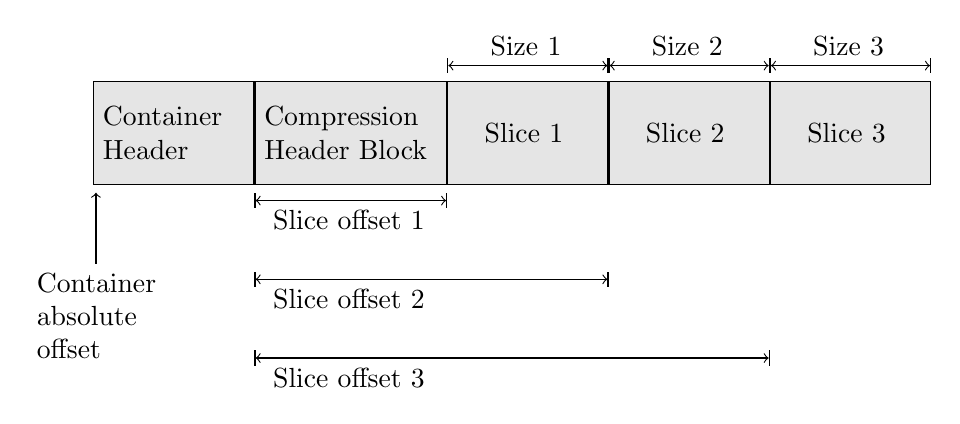
\begin{tikzpicture}[
  boxed/.style={rectangle, draw=black, fill=black!10, minimum height=1.3cm, text width=1.8cm},
]
\node(A) [boxed]{Container Header};
\node(B) [boxed,right,text width=2.2cm] at (A.east){Compression Header Block};
\node(C) [boxed,right] at (B.east){\quad Slice 1};
\node(D) [boxed,right] at (C.east){\quad Slice 2};
\node(E) [boxed,right] at (D.east){\quad Slice 3};

\draw[<-] (A.south west)+(1pt,-0.1cm) -- +(1pt,-1cm)
     node[below, text width=1.5cm]{Container absolute offset};


\draw[|<->|] ([yshift=-0.2cm]B.south west) node[below,xshift=1.2cm]{Slice offset 1}
    -- ([yshift=-0.2cm]B.south east);
\draw[|<->|] ([yshift=-1.2cm]B.south west) node[below,xshift=1.2cm]{Slice offset 2}
    -- ([yshift=-1.2cm]C.south east);
\draw[|<->|] ([yshift=-2.2cm]B.south west) node[below,xshift=1.2cm]{Slice offset 3}
    -- ([yshift=-2.2cm]D.south east);

\draw[|<->|] ([yshift=+0.2cm]C.north west) node[above,xshift=1cm]{Size 1} -- ([yshift=+0.2cm]C.north east);
\draw[|<->|] ([yshift=+0.2cm]D.north west) node[above,xshift=1cm]{Size 2} -- ([yshift=+0.2cm]D.north east);
\draw[|<->|] ([yshift=+0.2cm]E.north west) node[above,xshift=1cm]{Size 3} -- ([yshift=+0.2cm]E.north east);


\end{tikzpicture}
\end{center}

\subsubsection*{BAM index}

BAM indexes are supported by using 4-byte integer pointers called landmarks that 
are stored in container header. BAM index pointer is a 64-bit value with 48 bits 
reserved for the BAM block start position and 16 bits reserved for the in-block 
offset. When used to index CRAM files, the first 48 bits are used to store the 
CRAM container start position and the last 16 bits are used to store the index 
of the landmark in the landmark array stored in  container header. The landmark 
index can be used to access the appropriate slice. 

The above indexing scheme treats CRAM slices as individual records in BAM file. 
This allows to apply BAM indexing to CRAM files, however it introduces some overhead 
in seeking specific alignment start because all preceding records in the slice 
must be read and discarded.

\section{Encodings}
\label{sec:encodings}

% FIXME: we have a mishash of coding, encoding and codec.  We should
% go through the entire document and be consistent.

\subsection{Introduction}

The basic idea for encodings is to efficiently represent byte and integer values.
This can be achieved in a number of ways that most frequently involve some knowledge 
about the nature of the values being encoded, for example, distribution statistics. 
The methods for choosing the best encoding and determining its parameters are very 
diverse and are not part of the CRAM format specification, which only describes 
how the information needed to decode the values should be stored.

\subsection{BYTE}

This encoding simply stores byte values verbatim to a block with a given ID.

\subsubsection*{Parameters}

CRAM format defines the following parameters for BYTE encoding: 

\begin{tabular}{|>{\raggedright}p{100pt}|>{\raggedright}p{100pt}|>{\raggedright}p{230pt}|}
\hline
\textbf{Data type} & \textbf{Name} & \textbf{Comment}
\tabularnewline
\hline
uint7 & id & id of a block containing the byte stream\tabularnewline
\hline
\end{tabular}

\subsection{VARINT\_UNSIGNED}

This encoding stores unsigned integer values using the Variable Length Quantity
format (VLQ)\footnote{https://en.wikipedia.org/wiki/Variable-length\_quantity}.

It is not permitted to store any negative values using this encoding.
However given several data series have ranges that have the
possibility of small negative values (such as -1 for Alignment
Position), it is possible to skew the values slightly by adding an
offset prior to encoding.  This provides a mechanism for guaranteeing
all values remain positive.

Note this offset is added to the value after that value has been
decoded so to encode -1 we may wish to set offset to -1 and encode a
zero.  This mechanism may also be used to skew a range of values that
do not cluster around zero.  For example if a data series has values
ranging from 1000 to 1200, then setting offset to 1000 and encoding
values between 0 and 200 would provide a smaller data footprint.

For data series that require a broader scope of signed values we would
recommend using VARINT\_SIGNED instead.

\subsubsection*{Parameters}

CRAM format defines the following parameters for VARINT\_UNSIGNED encoding: 

\begin{tabular}{|>{\raggedright}p{100pt}|>{\raggedright}p{100pt}|>{\raggedright}p{230pt}|}
\hline
\textbf{Data type} & \textbf{Name} & \textbf{Comment}
\tabularnewline
\hline
sint7 & offset & amount to add to decoded values\tabularnewline
\hline
uint7 & id & id of a block containing the byte stream\tabularnewline
\hline
\end{tabular}

\subsection{VARINT\_SIGNED}

This encoding permits storing a broad range of both positive and
negative values while still following the property of low magnitude
values taking up less space than large magnitude ones.

It achieves this by using ZigZag encoding where signed values 0, -1,
+1, -2, +2 and so on are mapped to unsigned values 0, 1, 2, 3, 4.
These unsigned values are then stored using the same VLQ system used
by VARINT\_UNSIGNED.

As with VARINT\_UNSIGNED, an offset is added to the value after it has
been VLQ and ZigZag decoded.  Combined these permit efficient storage
of a distribution of values centred around a mean.  For example if
the distribution of values in a data series ranged from 1000 to 2000
with a peak at 1500, we could set offset to 1500 and encode values
-500 to +500.

\subsubsection*{Parameters}

CRAM format defines the following parameters for VARINT\_SIGNED encoding: 

\begin{tabular}{|>{\raggedright}p{100pt}|>{\raggedright}p{100pt}|>{\raggedright}p{230pt}|}
\hline
\textbf{Data type} & \textbf{Name} & \textbf{Comment}
\tabularnewline
\hline
sint7 & offset & amount to add to decoded values\tabularnewline
\hline
uint7 & id & id of a block containing the byte stream\tabularnewline
\hline
\end{tabular}


\subsection{CONST\_BYTE}

Sometimes a data series has a constant value throughout the
container.  In this case we can record this value in the Container
Compression Header and avoid the need to store the data series.

\subsubsection*{Parameters}

CRAM format defines the following parameters for CONST\_BYTE encoding: 

\begin{tabular}{|>{\raggedright}p{100pt}|>{\raggedright}p{100pt}|>{\raggedright}p{230pt}|}
\hline
\textbf{Data type} & \textbf{Name} & \textbf{Comment}
\tabularnewline
\hline
byte & value & the constant value\tabularnewline
\hline
\end{tabular}

\subsection{CONST\_INT}

As per CONST\_BYTE, but the value is a signed integer encoded with
VLQ and ZigZag methods.
The overhead of using ZigZag encoding on a constant unsigned value is
an average of 1 bit per container per use of this encoding.

\subsubsection*{Parameters}

CRAM format defines the following parameters for CONST\_INT encoding: 

\begin{tabular}{|>{\raggedright}p{100pt}|>{\raggedright}p{100pt}|>{\raggedright}p{230pt}|}
\hline
\textbf{Data type} & \textbf{Name} & \textbf{Comment}
\tabularnewline
\hline
sint & value & the constant value\tabularnewline
\hline
\end{tabular}

\subsection{BYTE\_ARRAY\_LEN (ID 4)}

Can encode types \textit{Byte[]}.

Often there is a need to encode an array of bytes where the length is
not predetermined.  For example the read identifiers differ per
alignment record, possibly with different lengths, and this length
must be stored somewhere.   Note in contrast to this, quality values
are known to be the same length as the sequence which is an already
known quantity, so the CRAM record encodes this using an implicit
array by asking for multiple values to be decoded rather than using an
explicit byte array encoding.

With BYTE\_ARRAY\_LEN the length is explicitly encoded via its own
sub-encoding prior to the array of bytes itself, also via its own
sub-encoding.

Note these sub-encodings may store the data in the same block, in
which case the length comes first. Alternatively we may decide that
the lengths have their own unique distribution which differs
substantially to the data itself and so should be stored in a
different block to permit better compression.  Having decoded the
length, the decoder must then call the value sub-encoding that many
times to retrieve the bytes.

Given the recursion used here of an encoding using two sub-encodings,
the byte stream for BYTE\_ARRAY\_LEN is the concatenation of both
sub-encodings.

\subsubsection*{Parameters}

The parameters for BYTE\_ARRAY\_LEN are listed below:

\begin{tabular}{|>{\raggedright}p{100pt}|>{\raggedright}p{100pt}|>{\raggedright}p{230pt}|}
\hline
\textbf{Data type} & \textbf{Name} & \textbf{Comment}
\tabularnewline
\hline
encoding\texttt{<}int\texttt{>} & lengths encoding & an encoding describing how 
the arrays lengths are stored\tabularnewline
\hline
encoding\texttt{<}byte\texttt{>} & values encoding & an encoding describing how 
the values (bytes) are stored\tabularnewline
\hline
\end{tabular}

\subsubsection*{Example}

The bytes for an X0:i SAM auxiliary field consisting of 16-bit items
may be written as an X0S tag line.  Despite the size being known, all
tag items are stored as byte arrays, so BYTE\_ARRAY\_LEN is ideal when
coupled with a CONST\_INT encoding to hold the fixed size lengths and
BYTE for the values.

\begin{tabular}{lll}
\hline
\textbf{Bytes} & & \textbf{Meaning}\\
\hline
\texttt{0x04}         & & BYTE\_ARRAY\_LEN encoding ID                                    \\
\texttt{0x07}         & & 7 remaining bytes of BYTE\_ARRAY\_LEN parameters            \\
\\
\texttt{0x44}         & & CONST\_INT encodng ID, for the aux tag lengths \\
\texttt{0x01}         & & remaining length of CONST\_INT encoding \\
\texttt{0x05}         & & length 2 as Zig-Zag format \\
\\
\texttt{0x01}         & & BYTE encoding ID, for the aux tag values \\
\texttt{0x02}         & & 2 more bytes of BYTE parameters                          \\
\texttt{0x81 0x48}    & & uint7 encoding for block ID 200                              \\
\hline
\end{tabular}

\subsection{BYTE\_ARRAY\_STOP (ID 5)}

Can encode types \textit{Byte[]}.

Instead of encoding an explicit length (as per BYTE\_ARRAY\_LEN) this
encoding stores bytes ending in a termination value.  The data
returned should not include this termination byte.  Hence this is
comparable to the C language string encoding, which uses a nul
character for termination, while BYTE\_ARRAY\_LEN is more similar to
the Pascal language string encoding.

Given this encoding is capturing the length within the same data
stream as the bytes, unlike BYTE\_ARRAY\_LEN this does not require
use of sub-encodings.  This makes it considerably simpler, but it has
redundancy when the stored arrays have constant lengths.

The choice of termination symbol is up to the encoder, but logical
choices may include the nul byte or the tab character as both are
illegal within SAM records.

\begin{tabular}{|>{\raggedright}p{100pt}|>{\raggedright}p{100pt}|>{\raggedright}p{230pt}|}
\hline
\textbf{Data type} & \textbf{Name} & \textbf{Comment}
\tabularnewline
\hline
byte & stop byte & a special byte treated as a delimiter\tabularnewline
\hline
uint7 & block id & id of a block containing the byte stream\tabularnewline
\hline
\end{tabular}

% \subsection{Beta coding: codec ID 6}
% 
% Can encode types \textit{Integer}.
% 
% \subsubsection*{Definition}
% 
% Beta coding is a most common way to represent numbers in \emph{binary notation} and is sometimes referred to as binary coding.
% The decoder reads the specified fixed number of bits (most significant first) and subtracts the offset value to get the decoded integer.
% 
% \subsubsection*{Parameters}
% 
% CRAM format defines the following parameters of beta coding: 
% 
% \begin{tabular}{|>{\raggedright}p{144pt}|>{\raggedright}p{144pt}|>{\raggedright}p{144pt}|}
% \hline
% \textbf{Data type} & \textbf{Name} & \textbf{Comment}\tabularnewline
% \hline
% itf8 & offset & offset is subtracted from each value during decode\tabularnewline
% \hline
% itf8 & length & the number of bits used\tabularnewline
% \hline
% \end{tabular}
% 
% \subsubsection*{Examples}
% 
% If we have integer values in the range 10 to 15 inclusive, the largest value would traditionally need 4 bits, but with an offset of -10 we can hold values 0 to 5, using a fixed size of 3 bits.
% Using fixed Offset and Length coming from the beta parameters, we decode these values as:
% 
% \begin{tabular}{|>{\raggedright}p{105pt}|>{\raggedright}p{105pt}|>{\raggedright}p{105pt}|>{\raggedright}p{105pt}|}
% \hline
% Offset & Length & \textbf{Bits} & \textbf{Value}\tabularnewline
% \hline
% -10 & 3 & 000 & 10\tabularnewline
% \hline
% -10 & 3 & 001 & 11\tabularnewline
% \hline
% -10 & 3 & 010 & 12\tabularnewline
% \hline
% -10 & 3 & 011 & 13\tabularnewline
% \hline
% -10 & 3 & 100 & 14\tabularnewline
% \hline
% -10 & 3 & 101 & 15\tabularnewline
% \hline
% \end{tabular}
% 
% \subsection{Subexponential coding: codec ID 7}
% 
% Can encode types \textit{Integer}.
% 
% \subsubsection*{Definition}
% 
% Subexponential coding\footnote{Fast progressive lossless image compression, Paul G. Howard and Jeffrey Scott Vitter, 1994. \url{http://www.ittc.ku.edu/~jsv/Papers/HoV94.progressive_FELICS.pdf}} is parametrized by a non-negative integer $k$.
% For values $n < 2^{k+1}$ subexponential coding produces codewords identical to Rice coding \footnote{\url{https://en.wikipedia.org/wiki/Golomb_coding\#Rice_coding}}.  For larger values it grows logarithmically with $n$.
% 
% \subsubsection*{Encoding}
% 
% \begin{enumerate}
% \item Add $\mathit{offset}$ to $n$.
% 
% \item Determine $u$ and $b$ values from $n$
% \begin{align*}
% b =
% \begin{cases}
%   \ k                        & \text{ if $n < 2^k$} \\
%   \ \lfloor log_{2}n \rfloor & \text{ if $n \ge 2^k$}
% \end{cases}
% &\
% &u =
% \begin{cases}
%   \ 0     & \text{ if $n < 2^k$} \\
%   \ b-k+1 & \text{ if $n \ge 2^k$}
% \end{cases}
% \end{align*}
% 
% \item Write $u$ in unary form; $u$ 1 bits followed by a single 0 bit.
% 
% \item Write the bottom $b$-bits of $n$ in binary form.
% \end{enumerate}
% 
% \subsubsection*{Decoding}
% 
% \begin{enumerate}
% \item Read $u$ in unary form, counting the number of leading 1s (prefix) in the codeword (discard the trailing 0 bit).
% 
% \item Determine $n$ via:
% \begin{enumerate}
% \item if $u = 0$ then read $n$ as a $k$-bit binary number.
% \item if $u \ge 1$ then read $x$ as a $(u + k - 1)$-bit binary. Let $n = 2^{u+k-1} + x$.
% \end{enumerate}
% 
% \item Subtract $\mathit{offset}$ from $n$.
% \end{enumerate}
% 
% \subsubsection*{Examples}
% 
% \begin{tabular}{|>{\raggedright}p{105pt}|>{\raggedright}p{105pt}|>{\raggedright}p{105pt}|>{\raggedright}p{105pt}|}
% \hline
% \textbf{Number} & \textbf{Codeword, k=0} & \textbf{Codeword, k=1} & \textbf{Codeword, 
% k=2}\tabularnewline
% \hline
% 0 & 0 & 00 & 000\tabularnewline
% \hline
% 1 & 10 & 01 & 001\tabularnewline
% \hline
% 2 & 1100 & 100 & 010\tabularnewline
% \hline
% 3 & 1101 & 101 & 011\tabularnewline
% \hline
% 4 & 111000 & 11000 & 1000\tabularnewline
% \hline
% 5 & 111001 & 11001 & 1001\tabularnewline
% \hline
% 6 & 111010 & 11010 & 1010\tabularnewline
% \hline
% 7 & 111011 & 11011 & 1011\tabularnewline
% \hline
% 8 & 11110000 & 1110000 & 110000\tabularnewline
% \hline
% 9 & 11110001 & 1110001 & 110001\tabularnewline
% \hline
% 10 & 11110010 & 1110010 & 110010\tabularnewline
% \hline
% \end{tabular}
% 
% \subsubsection*{Parameters}
% 
% \begin{tabular}{|>{\raggedright}p{100pt}|>{\raggedright}p{100pt}|>{\raggedright}p{230pt}|}
% \hline
% \textbf{Data type} & \textbf{Name} & \textbf{Comment}
% \tabularnewline
% \hline
% itf8 & offset & offset is subtracted from each value during decode\tabularnewline
% \hline
% itf8 & k & the order of the subexponential coding\tabularnewline
% \hline
% \end{tabular}
% 
% \subsection{Gamma coding: codec ID 9}
% 
% Can encode types \textit{Integer}.
% 
% \subsubsection*{Definition}
% 
% \emph{Elias gamma code} is a prefix encoding of positive integers. This is a combination 
% of unary coding and beta coding. The first is used to capture the number of bits 
% required for beta coding to capture the value. 
% 
% \subsubsection*{Encoding}
% 
% \begin{enumerate}
% \item Write it in binary.
% 
% \item Subtract $1$ from the number of bits written in step 1 and prepend that many zeros.
% 
% \item An equivalent way to express the same process:
% 
% \item Separate the integer into the highest power of $2$ it contains ($2N$) and the remaining 
% $N$ binary digits of the integer.
% 
% \item Encode $N$ in unary; that is, as $N$ zeroes followed by a one.
% 
% \item Append the remaining $N$ binary digits to this representation of $N$.
% \end{enumerate}
% 
% \subsubsection*{Decoding}
% 
% \begin{enumerate}
% \item Read and count 0s from the stream until you reach the first 1. Call this count 
% of zeroes $N$.
% 
% \item Considering the one that was reached to be the first digit of the integer, with 
% a value of $2N$, read the remaining $N$ digits of the integer.
% \end{enumerate}
% 
% \subsubsection*{Examples}
% 
% \begin{tabular}{|>{\raggedright}p{76pt}|>{\raggedright}p{107pt}|}
% \hline
% \textbf{Value} & \textbf{Codeword}\tabularnewline
% \hline
% 1 & 1\tabularnewline
% \hline
% 2 & 010\tabularnewline
% \hline
% 3 & 011\tabularnewline
% \hline
% 4 & 00100\tabularnewline
% \hline
% \end{tabular}
% 
% \subsubsection*{Parameters}
% 
% \begin{tabular}{|>{\raggedright}p{144pt}|>{\raggedright}p{144pt}|>{\raggedright}p{144pt}|}
% \hline
% \textbf{Data type} & \textbf{Name} & \textbf{Comment}\tabularnewline
% \hline
% itf8 & offset & offset to subtract from each value after decode\tabularnewline
% \hline
% \end{tabular}
% 
% \subsection{DEPRECATED: Golomb coding: codec ID 2}
% 
% Can encode types \textit{Integer}.
% 
% Note this codec has not been used in any known CRAM implementation since before CRAM v1.0.
% Nor is it implemented in some of the major software.
% Therefore its use is not recommended.
% 
% \subsubsection*{Definition}
% 
% \emph{Golomb encoding} is a prefix encoding optimal for representation of random 
% positive numbers following geometric distribution. 
% 
% \subsubsection*{Encoding}
% 
% \begin{enumerate}
% \item Fix the parameter $M$ to an integer value.
% 
% \item For $N$, the number to be encoded, find
% 
% \begin{enumerate}
% \item quotient $q = \lfloor N/M \rfloor$
% 
% \item remainder $r = N \bmod M$
% \end{enumerate}
% 
% \item Generate Codeword
% 
% \begin{enumerate}
% \item The Code format : \texttt{<}Quotient Code\texttt{>}\texttt{<}Remainder Code\texttt{>}, 
% where
% 
% \item Quotient Code (in unary coding)
% 
% \begin{enumerate}
% \item Write a $q$-length string of 1 bits
% 
% \item Write a 0 bit
% \end{enumerate}
% 
% \item Remainder Code (in truncated binary encoding)
% 
% Set $b=\lceil log_{2}(M) \rceil$
% 
% \begin{enumerate}
% \item If $r < 2^{b}-M$ code $r$ as plain binary using $b-1$ bits.
% 
% \item If $r \ge 2^{b}-M$ code the number $r+2^{b}-M$ in plain binary representation 
% using $b$ bits.
% \end{enumerate}
% \end{enumerate}
% \end{enumerate}
% 
% \subsubsection*{Decoding}
% 
% \begin{enumerate}
% \item Read $q$ via unary coding: count the number of 1 bits and consume the following 0 bits.
% \item Set $b=\lceil log_{2}(M) \rceil$
% \item Read $r$ via $b-1$ bits of binary coding
% \item If $r \ge 2^{b}-M$
% \begin{enumerate}
% \item Read 1 single bit, $x$.
% \item Set $r = r*2 + x - (2^{b}-M)$
% \end{enumerate}
% \item Value is $q*M + r - \mathit{offset}$
% \end{enumerate}
% 
% \subsubsection*{Examples}
% 
% \begin{tabular}{|>{\raggedright}p{76pt}|>{\raggedright}p{107pt}|}
% \hline
% \textbf{Number} & \textbf{Codeword, M=10, (thus b=4)}\tabularnewline
% \hline
% 0 & 0000\tabularnewline
% \hline
% 4 & 0100\tabularnewline
% \hline
% 10 & 10000\tabularnewline
% \hline
% 26 & 1101100\tabularnewline
% \hline
% 42 & 11110010\tabularnewline
% \hline
% \end{tabular}
% 
% \subsubsection*{Parameters}
% 
% Golomb coding takes the following parameters: 
% 
% \begin{tabular}{|>{\raggedright}p{144pt}|>{\raggedright}p{144pt}|>{\raggedright}p{144pt}|}
% \hline
% \textbf{Data type} & \textbf{Name} & \textbf{Comment}\tabularnewline
% \hline
% itf8 & offset & offset is added to each value\tabularnewline
% \hline
% itf8 & M & the golomb parameter (number of bins)\tabularnewline
% \hline
% \end{tabular}
% 
% \subsection{DEPRECATED: Golomb-Rice coding: codec ID 8}
% 
% Can encode types \textit{Integer}.
% 
% Note this codec has not been used in any known CRAM implementation since before CRAM v1.0.
% Nor is it implemented in some of the major software.
% Therefore its use is not recommended.
% 
% Golomb-Rice coding is a special case of Golomb coding when the M parameter is a power of 2.
% The reason for this coding is that the division operations in Golomb coding can be replaced with bit shift operators as well as avoiding the extra $r < 2^{b}-M$ check.

\section{Block compression methods}

Each block will hold different types of data and may have very
different characteristics for compression.  Hence CRAM can utilise
several different compression methods. Each method has an associated numeric code which is defined in Section~\ref{sec:block-struct}.

The following methods are defined.
Exact definitions of these methods are in their respective internet links or the ancillary \textit{CRAMcodecs} document found along side this specification.

\subsection{Gzip}

The Gzip specification is defined in RFC 1952.
Gzip in turn is an encapsulation on the Deflate algorithm defined in RFC 1951.

\subsection{Bzip2}

First available in CRAM v2.0.

Bzip2 is a compression method utilising the Burrows Wheeler Transform, Move To Front transform, Run Length Encoding and a Huffman entropy encoder. 
It is often superior to Gzip for textual data.

An informal format specification exists:\\
\url{https://github.com/dsnet/compress/blob/master/doc/bzip2-format.pdf}

\subsection{LZMA}

First available in CRAM v3.0.

LZMA is the Lempel-Ziv Markov chain algorithm.
CRAM uses the xz Stream format to encapsulate this algorithm, as defined in \url{https://tukaani.org/xz/xz-file-format.txt}.

\subsection{rANS4x8 codec}

First available in CRAM v3.0.

rANS is the range-coder variant of the Asymmetric Numerical
System\footnote{J. Duda, \textit{Asymmetric numeral systems: entropy
    coding combining speed of Huffman coding with compression rate of
    arithmetic coding}, \url{http://arxiv.org/abs/1311.2540}}.

``4x8'' refers to 4-way interleaving with 8-bit renormalisation.\newline
This variant of rANS first appeared in CRAM v3.0.

Details of this algorithm have been moved to the \textit{CRAMcodecs} document.

\subsection{rANS4x16 codec}

First available in CRAM v3.1.

``4x16'' refers to 4-way interleaving with 16-bit renormalisation.\newline
This variant of rANS first appeared in CRAM v3.1.

Details of this algorithm are listed in the \textit{CRAMcodecs} document.

\subsection{adaptive arithemtic coding}

First available in CRAM v3.1.

An entropy encoder that is slower but slightly more concise than
rANS.  It achieves this by adapting the probabilities as it compresses
and decompresses instead of using a fixed table.

Details of this algorithm are listed in the \textit{CRAMcodecs} document.

\subsection{fqzcomp codec}

First available in CRAM v3.1.

This is a method dedicated to compression of quality values.

Details of this algorithm are listed in the \textit{CRAMcodecs} document.

\subsection{name tokeniser}

First available in CRAM v3.1.

This is a method dedicated to compression of read names.

Details of this algorithm are listed in the \textit{CRAMcodecs} document.

\appendix
\renewcommand{\thesection}{\arabic{section}}

\newcommand{\appsection}[1]{%
  \addtocounter{section}{1}
  \section*{Appendix~\thesection \quad #1}
  \addcontentsline{toc}{section}{Appendix~\thesection \quad #1}
}

\appsection{Choosing the container size}

The CRAM format does not constrain the size of the containers.
However, the following should be considered when deciding the container size:

-- Data can be compressed better by using larger containers.

-- Random access performance is better for smaller containers.

-- Streaming is more convenient for small containers.

-- Applications typically buffer containers into memory.

-- Multi-threaded applications likely have a granularity of 1
container for each unit of work.

As a guidance, the default container size for htslib and htsjdk is one
slice of 10,000 short reads (fewer for long reads), but some users
find 1,000 is more appropriate if they need a lot of random access.

\appsection{CRAM 4.0 changes and rationale}
\label{sec:cram4changes}

CRAM 4.0 has a number of changes.  For those familier with the version
3.0 format, this is a list of changes along with a rationale for
making them.

\begin{description}
\item[New variable sized integer encoding]\ \newline
  Use VLQ (https://en.wikipedia.org/wiki/Variable-length\_quantity)
  instead of ITF8 and LTF8.

  This has the impact of not needing to distinguish between 32-bit and
  64-bit quantities, which we previously needed to do with ITF8 vs
  LTF8.  It also has a small reduction to compressed sizes.


\item[Long chromosome support]\ \newline
  A corollary of the removal of ITF8 and LTF8 means all fields
  can now be 64-bit if appropriate.  Importantly this removes the
  32-bit limit on the size of AP (alignment pos), TS (template size),
  NP (next mate pos).


\item[Signed numbers]\ \newline
  Variable sized integer encoding can now also do signed numbers.
  Previously -1 was stored as FF FF FF 0F (ITF8) and even more FFs
  for LTF8.  This is unwieldy and also bakes in knowledge of the
  size of the intended data type, making it impossible to increase
  data type sizes without changing the format.

  Signed fields are used for AP (alignment pos), TS (template size)
  and RG (read group, which can be -1 for not present).


\item[MD, NM presence and location]\ \newline
  CRAM derives MD and NM tags on-the-fly where possible.  However it
  doesn't record whether they were in the original data.

  The presence of MD and NM are now recorded, so if the input data didn't
  have them we won't reproduce on decode, and vice versa.  The
  location of MD, NM and RG in the tag stream are now also recorded,
  meaning CRAM 4.0 will round-trip more precisely.


\item[Quality value orientation]\ \newline
  On some technologies it is better to record qualities in their
  original orientation rather than the alignment orientation as this
  improves compression ratios.

  This is an optional setting in the compression header.  The data
  should be automatically flipped back during decode so the operation
  is transparent to the user.


\item[New CF explicit template size flag]\ \newline
  In CRAM RNEXT, PNEXT and TLEN are generated on-the-fly for read
  pairs residing in the same slice.  If we wish to preserve data
  verbatim for exceptions, such as TLEN off-by-one errors (common in
  old data) or TLEN 5' to 5' vs leftmost to rightmost differences then
  we had to mark the record as ``detached'' and store all 3 fields.

  We now have an flag to state that TLEN is explicitly stored without
  needing to use the CF detached flag.  This can have a substantial
  impact on file sizes for some older data sets.


\item[Deduplication of read names]\ \newline
  For read pairs residing in the same slice we can use the same logic
  we previously used for RNEXT, PNEXT and TLEN generation to also
  deduplicate read names so it only needs storing once.

  This roughly halves the size of uncompressed RN data series,
  reducing the compressed size.

{\color{gray}
\item[(For consideration) Removal of slices]\ \newline
  CRAM 3.0 offers the ability to have multiple slices per container.
  
  This is largely unused and does not provide the originally planned
  benefits of sharing compression meta-data between slices.  The
  defaults from both htslib and htsjdk are one slice per container.

  Removal of multi-slice containers, and by extension slices
  themselves, offers a simplified interface.

  An alternative to this is to permit another set of blocks prior to
  the first slice, with duplicate block IDs to those used in the
  slices.  These blocks pertain to the container and are utilised in
  unison with the per slice blocks.  For rANS they could hold the
  frequency tables, permitting this to be shared across slices.  For
  gzip or zstd they could hold a predefined dictionary, permitting
  more efficient compression of small blocks.  This may grant finer
  grained random access capability without suffering so much data
  expansion.
}

\item[TODO: add PACK, RLE and DELTA encodings]\ \newline

\item[TODO: sanitize read\_names\_included]\ \newline
  Given we now state a blank name will copy from the mate pair and
  auto-generate if not, there's no need for this field.  We can just
  store blank names and cull the whole RN in DecodeMateData vs in-line
  shenanigans.

\item[TODO: make all aux tags first class encoding objects]\ \newline
  Right now aux tags are basically byte arrays encoded as per BAM.
  This isn't so efficient.  For example an XX:S data series with
  values ranging 0 to 500 but with many more small values are a few
  large ones would be better encoded as VLQ than an array of 16-bit
  quantities.

\end{description}

\end{document}

\title{CRAM format specification (version 4.0)}
\author{samtools-devel@lists.sourceforge.net}
\date{\headdate}
\maketitle


\begin{quote}\small
The master version of this document can be found at
\url{https://github.com/samtools/hts-specs}.\\
This printing is version~\commitdesc\ from that repository,
last modified on the date shown above.
\end{quote}

\begin{center}
\textit{license: Apache 2.0}
\end{center}
\vspace*{1em}

\tableofcontents
\newpage

\section{Overview}

This specification describes the CRAM 4.0 format. 

CRAM has the following major objectives:

\begin{enumerate}
\item Significantly better lossless compression than BAM

\item Full compatibility with BAM

\item Effortless transition to CRAM from using BAM files

\item Support for controlled loss of BAM data
\end{enumerate}

The first three objectives allow users to take immediate advantage of the CRAM 
format while offering a smooth transition path from using BAM files. The fourth 
objective supports the exploration of different lossy compression strategies and 
provides a framework in which to effect these choices. Please note that the CRAM 
format does not impose any rules about what data should or should not be preserved. 

Data in CRAM is aggregated by data type (analogous to SAM columns)
known as Data Series and stored in blocks with each block compressed
using a choice of general purpose or custom compression codecs.
Sequence is typically encoded relative to a reference
sequence\footnote{Markus Hsi-Yang Fritz, Rasko Leinonen, Guy Cochrane,
  and Ewan Birney, \textbf{Efficient storage of high throughput DNA
    sequencing data using reference-based compression}, {\sl Genome
    Res.}~2011~21: 734--740;
  \href{http://dx.doi.org/doi:10.1101/gr.114819.110}{doi:10.1101/gr.114819.110};
  {\sc pmid:}21245279.}, but this is not a requirement.  Both aligned
and unaligned sequence is supported.

\section{Data types and formats}
\subsection*{Structures}

The CRAM format consists of header structures (container, compression, slice and block) and data series stored within the blocks themselves.
The fields of these structures use a mixture of fundamental types - boolean, byte, integer or array thereof - which are defined below.

% Types used in structures.
% Container:  uint, sint, uint[], byte[4](CRC), byte[]
% Block:      byte, uint, byte[], byte[4](CRC)
% CompHdr:    map, bool, byte[5], uint, byte[], encoding<>
% Slice:      sint, uint, uint[], byte[16], byte[]

\begin{tabular}{lll}
\textbf{Field type}  & \textbf{Format} & \textbf{Description}\\
\textit{bool}  & \textbf{byte} & A boolean, 0 (false) or 1 (true), stored as a byte. \\
\textit{byte}  & \textbf{byte} & An unsigned single byte (8 bits)  \\
\textit{uint}  & \textbf{VLQ\_unsigned} & A variable length integer $x >= 0$\\
\textit{sint}  & \textbf{VLQ\_signed}   & A variable length integer (may be negative)\\
\textit{array\texttt{<}type\texttt{>}} & \textbf{array} & An array of items of \textit{type} including the dimension\\
\\
\textit{type[]}  & \textit{as appropriate} & Zero or more items with unspecified length\\
\textit{type[4]} & \textit{as appropriate} & A constant number of items, dimension not stored\\
\end{tabular}
\vskip 10pt

The on-disk format for each of these encodings is listed below:

\begin{description}
\item[\textbf{byte}]\ \newline
A single byte

\item[\textbf{VLQ\_unsigned}]\ \newline
Integer values are encoded using Variable Length
Quantity\footnote{\url{https://en.wikipedia.org/wiki/Variable-length_quantity}}.

If the value is larger than 7-bits then the top-bit of the byte is
set, indicating a subsequent byte must be read.  This is repeated
until the top bit is unset. Bytes are written with the most
significant values first (big-endian format), which simplifies the
decode process.

Algorithmically this looks like:

\begin{algorithmic}[1]
\Statex
\Statex \textit{Read a variable sized unsigned integer 7-bits at a time.}
\Function{ReadUint7}{}
  \State $value \gets 0$
  \Repeat
    \State $c \gets$ \Call{ReadUint8}{}
    \State $value \gets (value \shiftl 7) + (c \bitand 127)$
  \Until{$c < 128$}
  \State \Return $value$
  \EndFunction
\end{algorithmic}

\item[\textbf{VLQ\_unsigned}]\ \newline
Signed integers are initially transformed to unsigned values using a zig-zag transformation, and then encoded as per unsigned values.
This maps signed values 0, -1, +1, -2, +2 to unsigned values 0, 1, 2, 3, 4 respectively, and vice versa during decode.

The zig-zag encoding method involves shifting the value left 1
bit and then XORing with all-bits-zero if positive or all-bits-one if
negative. I.e. $(v \shiftl 1) \bitxor (v \shiftr 31)$ for a
32-bit quantity using a 2's complement arithmetic shift right.

Decoding a zig-zag value is similar.  We XOR the value shifted right 1
bit with 0 or -1, taken from the negation of the bottom bit, as seen
below.

\begin{algorithmic}[1]
\Statex
\Statex \textit{Read a variable sized signed integer 7-bits at a time.}
\Function{ReadSint7}{}
  \State $value \gets $ \Call{ReadUint7}{}
  \State \Return $(value \shiftr 1) \bitxor -(value \bitand 1)$
  \EndFunction
\end{algorithmic}

\item[\textbf{array}]\ \newline
An array of items with the array dimension explicitly stored.
The array dimension is first, using VLQ\_signed format, followed by the array elements stored as per their \textit{type}.

\end{description}

Other custom data types exist, but will be introduced in the relevant sections.

\section{File Layout}

The basic structure of a CRAM file is a file header (magic number)
followed by a series of containers.  The first of these containers
holds textual meta-data (CRAM Header Container) and the last is used
as an end-of-file marker (CRAM EOF Container) with everyone inbetween
holding the sequence records themselves (Data Contaners).

\begin{center}
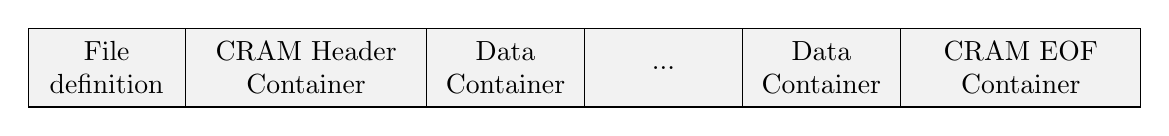
\begin{tikzpicture}[
  every node/.style={scale=1.0},
  boxes/.style={rectangle split,rectangle split parts=#1,draw,rectangle split horizontal,text width=5em,align=center,minimum height=1cm,fill=black!5,on grid},
  notes/.style={text width=20em,align=center,minimum height=1cm,on grid},
]
\node (file) [boxes=6] {
\nodepart{one}File definition
\nodepart[text width=8em]{two}CRAM Header Container
\nodepart{three}Data Container
\nodepart{four}...
\nodepart{five}Data Container
\nodepart[text width=8em]{six}CRAM EOF Container
};
\end{tikzpicture}

Figure 1: A CRAM file consists of a file definition, followed by a header container, then other containers.
\end{center}

Containers are just a Container Header Structure followed by one or
more Blocks.  Blocks have different types (see
~\ref{subsec:block-content-types}) corresponding to their usage.
Note the block itself also consists of a defined structure followed by
the block contents data.

\begin{center}
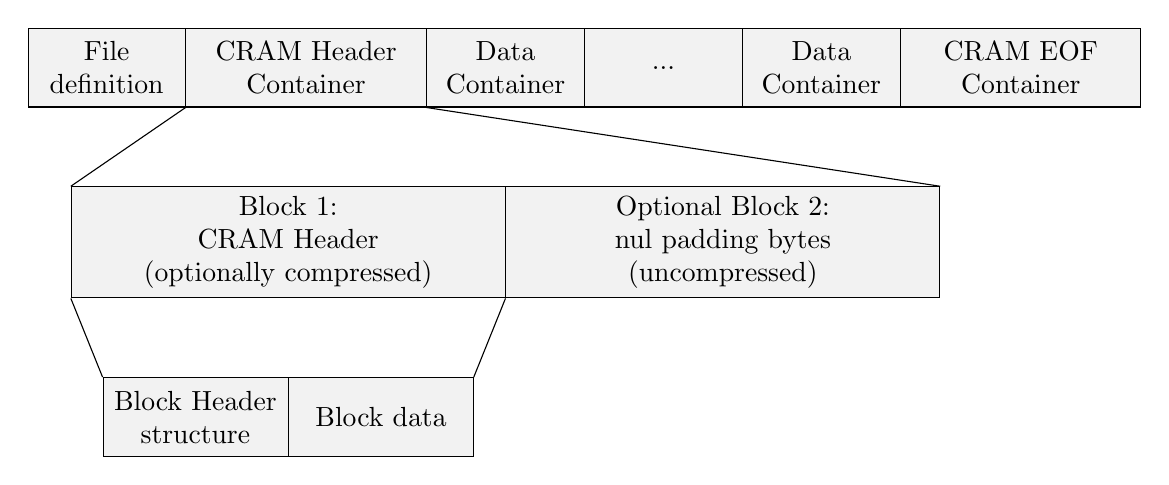
\begin{tikzpicture}[
  every node/.style={scale=1.0},
  boxes/.style={rectangle split,rectangle split parts=#1,draw,rectangle split horizontal,text width=5em,align=center,minimum height=1cm,fill=black!5,on grid},
  notes/.style={text width=20em,align=center,minimum height=1cm,on grid},
]
\node (file) [boxes=6] {
\nodepart{one}File definition
\nodepart[text width=8em]{two}CRAM Header Container
\nodepart{three}Data Container
\nodepart{four}...
\nodepart{five}Data Container
\nodepart[text width=8em]{six}CRAM EOF Container
};

\node (header) [boxes=2,below=1 of file.three south, text width=15em] {
\nodepart{one}Block 1:\break
CRAM Header\break
(optionally compressed)
\nodepart{two}Optional Block 2:\break
nul padding bytes\break
(uncompressed)
};
\draw (file.one split south) to (header.north west);
\draw (file.two split south) to (header.north east);

\node (blocks) [boxes=2,below=1 of header.one south,text width=6em] {
\nodepart{one}Block Header structure
\nodepart{two}Block data
};
\draw (header.south west) to (blocks.north west);
\draw (header.two split south) to (blocks.north east);
\end{tikzpicture}

Figure 2: The the first container holds the CRAM header text.
\end{center}

The first container, called the CRAM header container, is used to
store a textual header as described in the SAM specification (see the
section 7.1).  This is optionally followed by another uncompressed
block of nul padding bytes.  The purpose of this additional block is
to permit in-situ modification of the CRAM header without the
requirement to rewrite the entire file (instead needing just this
container to be rewritten, provided it can be padded to an identical
size).

\begin{center}
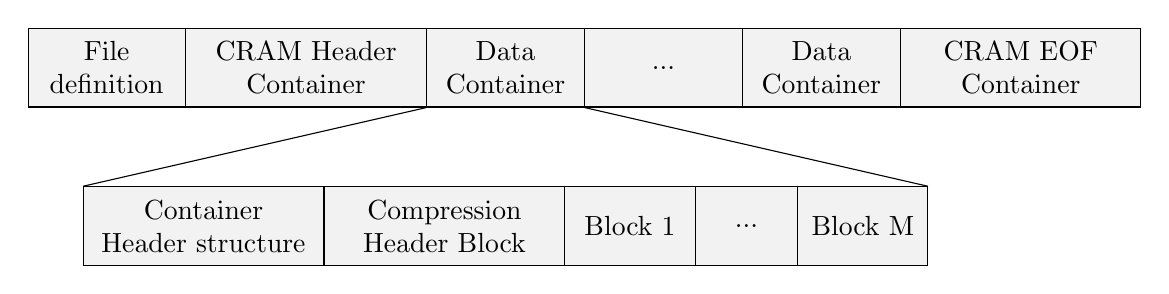
\begin{tikzpicture}[
  every node/.style={scale=1.0},
  boxes/.style={rectangle split,rectangle split parts=#1,draw,rectangle split horizontal,text width=5em,align=center,minimum height=1cm,fill=black!5,on grid},
  notes/.style={text width=20em,align=center,minimum height=1cm,on grid},
]
\node (file) [boxes=6] {
\nodepart{one}File definition
\nodepart[text width=8em]{two}CRAM Header Container
\nodepart{three}Data Container
\nodepart{four}...
\nodepart{five}Data Container
\nodepart[text width=8em]{six}CRAM EOF Container
};

\node (container) [boxes=5,below=1 of file.three south,text width=8em] {
\nodepart{one}Container Header structure
\nodepart{two}Compression Header Block
\nodepart[text width=4em]{three}Block 1
\nodepart[text width=3em]{four}...
\nodepart[text width=4em]{five}Block M
};
\draw (file.two split south) to (container.north west);
\draw (file.three split south) to (container.north east);
\end{tikzpicture}

Figure 3: Containers as a series of blocks
\end{center}

The Data Containers hold the sequence records themselves.
These start with a Compression Header block which holds meta-data
describing how and where the Data Series are encoded within this
container.

\begin{center}
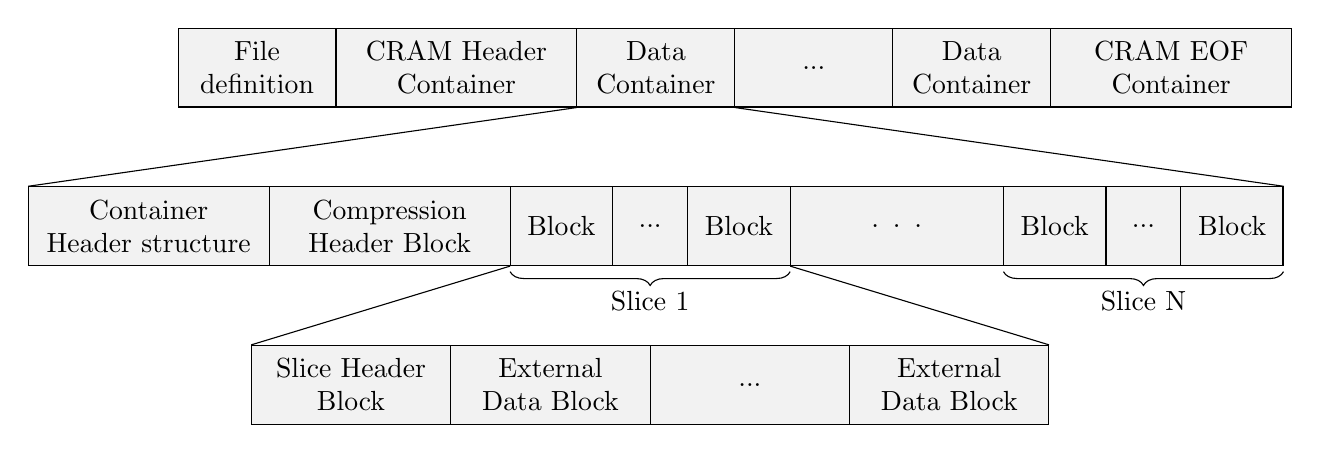
\begin{tikzpicture}[
  every node/.style={scale=1.0},
  boxes/.style={rectangle split,rectangle split parts=#1,draw,rectangle split horizontal,text width=5em,align=center,minimum height=1cm,fill=black!5,on grid},
  notes/.style={text width=20em,align=center,minimum height=1cm,on grid},
]
\node (file) [boxes=6] {
\nodepart{one}File definition
\nodepart[text width=8em]{two}CRAM Header Container
\nodepart{three}Data Container
\nodepart{four}...
\nodepart{five}Data Container
\nodepart[text width=8em]{six}CRAM EOF Container
};

\node (container) [boxes=9,below=1 of file.three south,text width=8em] {
\nodepart{one}Container Header structure
\nodepart{two}Compression Header Block
\nodepart[text width=3em]{three}Block
\nodepart[text width=2em]{four}...
\nodepart[text width=3em]{five}Block
\nodepart[text width=7em]{six}. . .
\nodepart[text width=3em]{seven}Block
\nodepart[text width=2em]{eight}...
\nodepart[text width=3em]{nine}Block
};
\draw (file.two split south) to (container.north west);
\draw (file.three split south) to (container.north east);

\draw[decoration={brace,mirror,amplitude=5pt,raise=2pt},decorate]
  (container.two split south) to (container.five split south);
\node [below=0.2 of container.four south] {Slice 1};

\draw[decoration={brace,mirror,amplitude=5pt,raise=2pt},decorate]
  (container.six split south) to (container.south east);
\node [below=0.2 of container.eight south] {Slice N};

\node (slice) [boxes=4,below=1 of container.four south, text width=6.5em] {
\nodepart{one}Slice Header Block
\nodepart{two}External Data Block
\nodepart{three}...
\nodepart{four}External Data Block
};
\draw (container.two split south) to (slice.north west);
\draw (container.five split south) to (slice.north east);
\end{tikzpicture}

Figure 4: Slices formed from a series of concatenated blocks
\end{center}

The blocks after the compression header are organised logically into slices. One 
slice may contain, for example, a contiguous region of alignment data. Slices begin 
with a slice header block and are followed by one or more data blocks.
It is these data blocks which hold the primary bulk of CRAM data, the
Data Series.

Note many CRAM files will just use one slice per contaner as this is
the default output format of several major implementations.

\subsection{File definition}

Each CRAM file starts with a fixed length (26 bytes) definition with the following 
fields:

\begin{tabular}{|l|l|l|}
\hline
\textbf{Data type} & \textbf{Name} & \textbf{Value}\tabularnewline
\hline
byte[4] & format magic number & CRAM (0x43 0x52 0x41 0x4d)\tabularnewline
\hline
byte & major format number & 3 (0x3)\tabularnewline
\hline
byte & minor format number & 1 (0x1)\tabularnewline
\hline
byte[20] & file id & CRAM file identifier (e.g. file name or SHA1 checksum)\tabularnewline
\hline
\end{tabular}

Valid CRAM \textit{major}.\textit{minor} version numbers are as follows:

\begin{itemize}
\item[\textit{1.0}]
The original public CRAM release.

\item[\textit{2.0}]
The first CRAM release implemented in both Java and C; tidied up
implementation vs specification differences in \textit{1.0}.

\item[\textit{2.1}]
Gained end of file markers; compatible with \textit{2.0}.

\item[\textit{3.0}]
Additional compression methods; header and data checksums;
improvements for unsorted data.

\item[\textit{3.1}]
Additional block compression codecs only.

\item[\textit{4.0}]
This specification.  Revised variable sized integers, MD/NM/RG tag
locators, and deduplication of read names.  Removed some encodings.
See \ref{sec:cram4changes} for a more detailed list of changes.
\end {itemize}

CRAM 3.0 and 3.1 differ only in the list of compression
methods available, so tools that output CRAM 3 without using any 3.1
codecs should write the header to indicate 3.0 in order to permit
maximum compatibility.

\subsection{Container header structure}

The file definition is followed by one or more containers with the following header 
structure where the container content is stored in the `blocks' field:

\begin{tabular}{|l|>{\raggedright}p{120pt}|>{\raggedright}p{260pt}|}
\hline
\textbf{Data type} & \textbf{Name} & \textbf{Value}
\tabularnewline
\hline
uint7 & length & the sum of the lengths of all blocks in this container (headers and data);
equal to the total byte length of the container minus the byte length of this header structure\tabularnewline
\hline
int7 & reference sequence id & reference sequence identifier  or\linebreak{}
-1 for unmapped reads\linebreak{}
-2 for multiple reference sequences.\linebreak{}
All slices in this container must have a reference sequence id matching this value.\tabularnewline
\hline
uint7 & starting position on the reference & the alignment start position or\linebreak{}
0 if the container is multiple-reference
or contains unmapped unplaced reads\tabularnewline
\hline
uint7 & alignment span & the length of the alignment or\linebreak{}
0 if the container is multiple-reference
or contains unmapped unplaced reads\tabularnewline
\hline
uint7 & number of records & number of records in the container\tabularnewline
\hline
uint7 & record counter & 1-based sequential index of records in the file/stream.\tabularnewline
\hline
uint7 & bases & number of read bases\tabularnewline
\hline
uint7 & number of blocks & the total number of blocks in this container\tabularnewline
\hline
array<uint7> & landmarks & the locations of slices in this container as byte offsets from the end of 
this container header, used for random access indexing.
The landmark count must equal the slice count.\linebreak{}
Since the block before the first slice is the compression header,
landmarks[0] is equal to the byte length of the compression header.\tabularnewline
\hline
uint32 & crc32 & CRC32 hash of the all the preceding bytes in the container.\tabularnewline
\hline
byte[ ] & blocks & The blocks contained within the container.\tabularnewline
\hline
\end{tabular}

\subsubsection*{CRC32}
This is a cyclic redundancy checksum 32-bit long with the polynomial 0x04C11DB7. Please refer to \href{http://www.itu.int/rec/recommendation.asp?type=folders&lang=e&parent=T-REC-V.42}{ITU-T V.42} for more details. The value of the CRC32 hash function is written as an integer.


\subsection{Block structure}
\label{sec:block-struct}

Containers consist of one or more blocks. Block compression is applied independently 
and in addition to any encodings used to compress data within the block. The block 
have the following header structure with the data stored in the `block data' field:

\begin{tabular}{|l|>{\raggedright}p{120pt}|>{\raggedright}p{260pt}|}
\hline
\textbf{Data type} & \textbf{Name} & \textbf{Value}
\tabularnewline
\hline
byte & method & the block compression method (and first CRAM version): \linebreak{}
0: raw (none)*\linebreak{}
1: gzip\linebreak{}
2: bzip2 (v2.0)\linebreak{}
3: lzma (v3.0)\linebreak{}
4: rans4x8 (v3.0)\linebreak{}
5: rans4x16 (v3.1)\linebreak{}
6: adaptive arithmetic coder (v3.1)\linebreak{}
7: fqzcomp (v3.1)\linebreak{}
8: name tokeniser (v3.1)
\tabularnewline
\hline
byte & block content type id & the block content type identifier\tabularnewline
\hline
uint7 & block content id & the block content identifier used to associate
data blocks with data series\tabularnewline
\hline
uint7 & size in bytes* & size of the block data after applying block compression\tabularnewline
\hline
uint7 & raw size in bytes* & size of the block data before applying block compression\tabularnewline
\hline
byte[ ] & block data & the data stored in the block\tabularnewline
\hline
uint32 & CRC32 & CRC32 hash value for all preceding bytes in the block\tabularnewline
\hline
\end{tabular}

* Note on raw method: both compressed and raw sizes must be set to the same value.

\subsubsection*{Block content types}
\label{subsec:block-content-types}

CRAM has the following block content types:

\begin{threeparttable}[t]
\begin{tabular}{|>{\raggedright}p{143pt}|>{\raggedright}p{45pt}|>{\raggedright}p{116pt}|>{\raggedright}p{114pt}|}
\hline
\textbf{Block content type} & \textbf{Block content type id} & \textbf{Name} & \textbf{Contents}\tabularnewline
\hline
FILE\_HEADER & 0 & CRAM header block & CRAM header\tabularnewline
\hline
COMPRESSION\_HEADER & 1 & Compression header block & See specific section\tabularnewline
\hline
SLICE\_HEADER & 2 & Slice header block & See specific section\tabularnewline
\hline
 & 3 &  & reserved\tabularnewline
\hline
EXTERNAL\_DATA & 4 & data block & data produced by encodings\tabularnewline
\hline
\end{tabular}
\end{threeparttable}

\subsubsection*{Block content id}

Block content id is used to distinguish between data blocks in the same slice. 
Each encoding has an id parameter which must be one of the block
content ids. For data blocks the content id is a positive integer. For all
other blocks content id should be 0. Consequently, all data encodings must 
not use content id less than 1. 

\subsection{CRAM header container}

The first container in a CRAM file contains a textual header in a single block, optionally
gzip compressed. This text header currently matches the SAM header specification. Only
gzip is allowed as compression method for this block. The CRAM header container does not
include a compression header block.

The following constraints apply to the SAM header: 

\begin{itemize}
\item The SQ:MD5 checksum is required unless the reference sequence has been embedded 
into the file.
\end{itemize}

It is recommended to reserve 50\% more space in the CRAM header container than
is required for the SAM header text by optionally padding the container with a second
raw block consisting of all zeroes. This can be used to subsequently expand the header
container in place, such as when updating @SQ records, while preserving the absolute
offsets of all subsequent containers.

\subsection{Compression header block}
\label{subsec:compression-header}

The compression header block consists of 3 parts: preservation map, data series 
encoding map and tag encoding map.  See below for the data format of a map.

These are meta-data on what is stored in the following slices, how it is encoded, and in which blocks the raw byte streams from these encodings reside.

\begin{tabular}{|l|>{\raggedright}p{120pt}|>{\raggedright}p{260pt}|}
\hline
\textbf{Data type} & \textbf{Name} & \textbf{Value}
\tabularnewline
\hline
map & preservation map & meta-data about types of data stored and dictionaries \tabularnewline
\hline
map & data series encoding map & meta-data for how data series are encoded \tabularnewline
\hline
map & tag encoding map & meta-data for how tags are encoded \tabularnewline
\hline
\end{tabular}

\subsubsection{Map structure}

% FIXME: is this better defined as a sub-structure in the relevant section itself?
% Possibly...
A \textit{Map} is a collection of keys and associated values.

Both the size in bytes and the number of keys are written as integer (uint7). Keys 
and values are written according to their data types and are specific to each map.
Keys have a fixed size for all items in a map, but this size is not
the same for all map types.  The order of keys is not defined.  Values
are stored immediately after their key in a key-defined format.  Some
keys will have simple boolean values, some are fixed size, while
others have a more complex sub-structures.

The example below is for a two byte key map.

\begin{tabular}{|l|>{\raggedright}p{120pt}|>{\raggedright}p{260pt}|}
\hline
\textbf{Data type} & \textbf{Name} & \textbf{Value}
\tabularnewline
\hline
uint7 & size & the remaining size in bytes of this map structure\tabularnewline
\hline
uint7 & num\_keys & the number of key-value pairs in this map\tabularnewline
\hline
byte[2] & key & first key\tabularnewline
\hline
byte[] & value & first value, with a key-specific size (see below).\tabularnewline
\hline
... & ... & \textit{repeated num\_keys time}\tabularnewline
\hline
\end{tabular}


\subsubsection{Preservation map}

The preservation map contains information about which data was preserved in the 
CRAM file. It is stored as a map with byte[2] keys:

\begin{tabular}{|l|l|>{\raggedright}p{100pt}|>{\raggedright}p{220pt}|}
\hline
\textbf{Key} & \textbf{Value data type} & \textbf{Name} & \textbf{Value}\tabularnewline
\hline
RN & bool & read names included & true if read names are preserved for all reads\tabularnewline
\hline
AP & bool & AP data series delta & true if AP data series is delta, false otherwise\tabularnewline
\hline
RR & bool & reference required & true if reference sequence is required to restore 
the data completely\tabularnewline
\hline
SM & byte[5] & substitution matrix & substitution matrix\tabularnewline
\hline
TD & array\texttt{<}byte\texttt{<>} & tag ids dictionary & a list of lists of tag ids, see tag encoding 
section\tabularnewline
\hline
QO & bool & qual orientation & true if quality values are in the same orientation as sequence.  If false quality values are recorded in the orientation as produced by the sequencing instrument, which may also still match sequence orientation.\tabularnewline
\hline
\end{tabular}

The boolean values are optional, defaulting to true when absent, although it is recommended to explicitly set them.  SM and TD are mandatory.

\subsubsection{Encoding structure}

The data series encoding map utilises another custom data type, \textit{encoding\texttt{<}type\texttt{>}}.
This is used to describe the data encapsulation format for a specific data series; how and where the values are stored.  This could be
the definition of a constant, a series of data transformations, or the
block content id for a data block.  Some encodings may be nested,
such as \texttt{BYTE\_ARRAY\_LEN} which defines one sub-encoding for the
length and another for the bytes.

Encoding notation is defined as the keyword `encoding' followed by its data type in angular brackets, for example `encoding\texttt{<}byte\texttt{>}' stands for an encoding that operates on a data series of data type `byte'.
Note there are distinct encodings dealing with signed and unsigned
data in addition to offsets applies to each, so for integer data the
data series use `encoding\texttt{<}int\texttt{>}` and let the specific
encoding and meta-data handle the sign as appropriate.

The \textit{encoding} format consists of an encoding type and type specific meta-data stored as an array (dimension followed by the array elements).

\begin{tabular}{|l|>{\raggedright}p{120pt}|>{\raggedright}p{260pt}|}
\hline
\textbf{Data type} & \textbf{Name} & \textbf{Value}
\tabularnewline
\hline
uint7 & encoding\_ID & encoding type identifier\tabularnewline
\hline
array\texttt{<}byte\texttt{>} & encoding\_meta & type specific meta-data for this encoding, serialised as a byte stream\tabularnewline
\hline
\end{tabular}

\vskip 10pt

Note unlike the fields in structures, data series types here do not
distinguish signed integer (sint) vs unsigned integer (uint) as this
distinction is handled by the encoding itself.  This is different to
CRAM 3.0 and earlier where the sign and size of the data series types
was written into the specification, rather than stored as meta-data in
the CRAM file.

For example, the alignment position (\textbf{AP}) data series has a value data type of \textit{encoding<int>}.
Typically on a position sorted file this is delta encoded and all
values are positive, so a suitable encoding is VARINT\_UNSIGNED.  If
the slice contains data aligned against multiple reference sequences
then this may contain some negative deltas in which case
VARINT\_SIGNED could be appropriate.

A list of data types along with their possible encodings is listed
below.

\begin{tabular}{llll}
\textbf{ID}  & \textbf{Encoding} & \textbf{Data Type} & \textbf{Description}\\
\hline
\\
0  & NULL             & \textit{N/A} & Data series not present\\
\\
1  & BYTE (EXTERNAL)  & byte   & An unsigned single byte (8 bits)  \\
\\
4  & BYTE\_ARRAY\_LEN & byte[] & Zero or more items with unspecified length\\
5  & BYTE\_ARRAY\_STOP& byte[] & Zero or more items with unspecified length\\
\\
41 & VARINT\_UNSIGNED & int    & A variable length integer (VLQ $x >= 0$)\\
42 & VARINT\_SIGNED   & int    & A variable length integer (VLQ, may be negative)\\
\\
43 & CONST\_BYTE      & byte   & A fixed byte value\\
44 & CONST\_INT       & int    & A fixed integer value (VLQ, signed)\\
\end{tabular}

\vskip 10pt

See section~\ref{sec:encodings} for more detailed descriptions of all
the above coding algorithms and their parameters.  Note the encoding
ID values here have been chosen to not clash with CRAM 3.0 and earlier
with the exception of the BYTE\_ARRAY\_LEN and BYTE\_ARRAY\_STOP
encodings which have not changed and BYTE which is identical and
synonymous with EXTERNAL in the CRAM 3.0 specification.

\subsubsection{Data series encoding map}

Writing to and reading from data blocks is organised through CRAM
records. A CRAM record is analogous to a single line in a SAM file.

The records are organised into slices and then each slice is
rearranged in a columnar fashion into data series.  For example
collect 10,000 SAM records and then the first column, query name
(QNAME), becomes one CRAM data series (RN), the next column (FLAG)
becomes CRAM data series (BF), and so on.  Note some SAM columns, such
as CIGAR, may map to many CRAM data series.

Each data series is associated with an encoding. An encoding may have
a block content id which is used to identify the block where the data
series is stored. Please note that data blocks can have multiple
data series associated with them; in this case the values from these
data series will be interleaved and must be decoded in the correct order.

\begin{center}
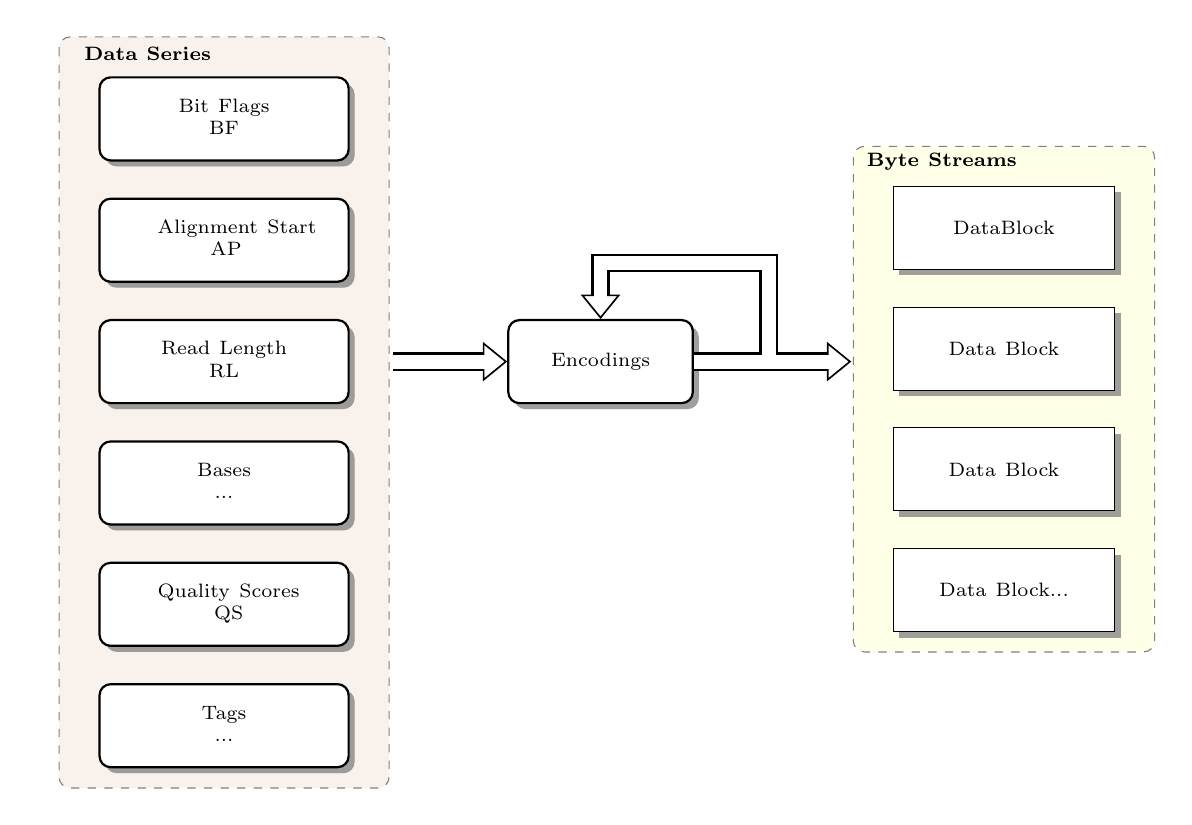
\begin{tikzpicture}[thick]

\usetikzlibrary{shapes, shadows, positioning, arrows,  decorations.markings, arrows.meta}

\pgfdeclarelayer{background}
\pgfsetlayers{background,main}

\tikzstyle{dsbox} = [blockbox, text width=6em, minimum width=9em, minimum height=3em, rounded corners, drop shadow]
\tikzstyle{blockbox}=[draw, fill=white, text width=4.0em, text centered, minimum height=1.0em, drop shadow]
\tikzstyle{encodedblock} = [blockbox, text width=6em, minimum width=8em, minimum height=3em, drop shadow]
\tikzstyle{encodings} = [dsbox, minimum width=6em, thick]

\tikzstyle{texto} = [above, text width=8em, text centered]

\tikzstyle{vecArrow} = [thick, decoration={markings,mark=at position
   1 with {\arrow[semithick]{Triangle[open, length=3.1mm, width=5mm]}}},
   double distance=5pt, shorten >= 8.5pt,
   preaction = {decorate},
   postaction = {draw,line width=5pt, white,shorten >= 8pt}]
\tikzstyle{innerWhite} = [semithick, white,line width=5pt, shorten >= 8pt]

\newcommand{\cramRecord}[6]{%
\begin{pgfonlayer}{background}
    \path (#1.west |- #1.north) + (-0.5, 0.5) node (a1) {};
    \path (#1.east |- #6.south) + (+0.5,-0.25) node (a2) {};
    \path[fill=brown!10,rounded corners, draw=black!50, dashed]
      (a1) rectangle (a2);
    \path (a1.east |- a1.south) + (1.0,-0.3) node[texto]
    {\scriptsize\textbf{Data Series}};
\end{pgfonlayer}}

\newcommand{\dsbox}[2]{node (p#1) [dsbox]
{\scriptsize{#2}}}
\newcommand{\encodedblock}[2]{node (p#1) [encodedblock]
	{\scriptsize{#2}}}
\newcommand{\encodedblocklarge}[2]{node (p#1) [encodedblocklarge]
   {\scriptsize{#2}}}

\path +(-2.5,-1.5) \dsbox{1}{\begin{tabular}{c} Bit Flags \\ BF \end{tabular}};
\path (p1.south)+(0.0,-1.0) \dsbox{2}{\begin{tabular}{c} Alignment Start\\ AP\quad\quad \end{tabular}};
\path (p2.south)+(0.0,-1.0) \dsbox{3}{\begin{tabular}{c} Read Length \\ RL \end{tabular}};
\path (p3.south)+(0.0,-1.0) \dsbox{4}{\begin{tabular}{c} Bases \\ ... \end{tabular}};
\path (p4.south)+(0.0,-1.0) \dsbox{5}{\begin{tabular}{c} Quality Scores \\ QS \end{tabular}};
\path (p5.south)+(0.0,-1.0) \dsbox{6}{\begin{tabular}{c} Tags \\ ... \end{tabular}};

\cramRecord{p1}{p2}{p3}{p4}{p5}{p6}

\newcommand{\blockStreams}[4]{%
\begin{pgfonlayer}{background}
    \path (#1.west |- #1.north)+(-0.5, 0.5) node (a3) {};
    \path (#4.east |- #4.south)+(+0.5, -0.25) node (a4) {};
    \path[fill=yellow!10, rounded corners, draw=black!50, dashed]
      (a3) rectangle (a4);
    \path (a3.east |- a3.south)+(1.0,-0.3) node[texto]{\scriptsize\textbf{Byte Streams}};
\end{pgfonlayer}}

\path (a1.south) + (12.0, -2.3) \encodedblock {7} {DataBlock};
\path (p7.south) + (0.0, -1.0)  \encodedblock {8} {Data Block};
\path (p8.south) + (0.0, -1.0)  \encodedblock {9} {Data Block}; 
\path (p9.south) + (0.0, -1.0)  \encodedblock {10}{Data Block...};

\blockStreams {p7} {p8} {p9} {p10}

\node (encodings) [encodings, right = 2 of p3] {\scriptsize Encodings};
\node (enc_e1) [right=0.7 of encodings] {};
\node (enc_e2) [right=1.05 of enc_e1] {};
\node (enc_n)  [above=1 of encodings.center] {};
\draw[vecArrow] (p3.east) + (0.55, 0) to (encodings.west);
\draw[vecArrow] (encodings.east) to (enc_e2.west);
\draw[vecArrow] (enc_e1.east) |- (enc_n.north) to (encodings.north);
\draw[innerWhite] (encodings.east) to (enc_e2.west);

\end{tikzpicture}

Figure 5: The relationship between Data Series, Possibly nested Encodings, and Data Blocks.

\end{center}

The picture shows how a CRAM record (on the left) is distributed to
multiple Data Blocks via a series of encodings.  Note the mapping from
Data Series to Blocks may be many to many, with the possibility of
multiple Data Series writing to the same Block and with a single
encoding such as BYTE\_ARRAY\_LEN potentially writing to two Blocks.


Each data series has an encoding. These encodings are stored in a map with byte[2] 
keys and are decoded in approximately this order\footnote{The precise order is defined in section~\ref{sec:record}.}:

\begin{threeparttable}[t]
\begin{tabular}{|l|l|>{\raggedright}p{100pt}|>{\raggedright}p{220pt}|}
\hline
\textbf{Key} & \textbf{Value data type} & \textbf{Name} & \textbf{Value}\tabularnewline
\hline
BF & encoding\texttt{<}int\texttt{>} & BAM bit flags & see separate section\tabularnewline
\hline
CF & encoding\texttt{<}int\texttt{>} & CRAM bit flags & see specific section\tabularnewline
\hline
RI & encoding\texttt{<}int\texttt{>} & reference id & record reference id from
the SAM file header\tabularnewline
\hline
RL & encoding\texttt{<}int\texttt{>} & read lengths & read lengths\tabularnewline
\hline
AP & encoding\texttt{<}int\texttt{>} & in-seq positions & if \textbf{AP-Delta} = true: 0-based alignment start
delta from the AP value in the previous record.
Note this delta may be negative, for example when switching references in a multi-reference slice.
When the record is the first in the slice, the previous position used is the slice alignment-start field (hence the first delta should be zero for single-reference slices, or the AP value itself for multi-reference slices).  \linebreak{}
if \textbf{AP-Delta} = false: encodes the alignment start position directly\tabularnewline
\hline
RG & encoding\texttt{<}int\texttt{>} & read groups & read groups. Special value 
`-1' stands for no group.\tabularnewline
\hline
RN\tnote{a} & encoding\texttt{<}byte[ ]\texttt{>} & read names & read names\tabularnewline
\hline
MF & encoding\texttt{<}int\texttt{>} & next mate bit flags & see specific section\tabularnewline
\hline
NS & encoding\texttt{<}int\texttt{>} & next fragment reference sequence id & reference 
sequence ids for the next fragment \tabularnewline
\hline
NP & encoding\texttt{<}int\texttt{>} & next mate alignment start & alignment positions 
for the next fragment\tabularnewline
\hline
TS & encoding\texttt{<}int\texttt{>} & template size & template sizes\tabularnewline
\hline
NF & encoding\texttt{<}int\texttt{>} & distance to next fragment & number of records
to the next fragment\tnote{b}\tabularnewline
\hline
TL\tnote{c} & encoding\texttt{<}int\texttt{>} & tag ids  & list of tag ids, see tag encoding
section\tabularnewline
\hline
FN & encoding\texttt{<}int\texttt{>} & number of read features & number of read
features in each record\tabularnewline
\hline
FC & encoding\texttt{<}byte\texttt{>} & read features codes & see separate section\tabularnewline
\hline
FP & encoding\texttt{<}int\texttt{>} & in-read positions & positions of the read
features; a positive delta to the last position (starting with zero)\tabularnewline
\hline
DL & encoding\texttt{<}int\texttt{>} & deletion lengths & base-pair deletion lengths\tabularnewline
\hline
BB & encoding\texttt{<}byte[ ]\texttt{>} & stretches of bases & bases\tabularnewline
\hline
QQ & encoding\texttt{<}byte[ ]\texttt{>} & stretches of quality scores & quality scores\tabularnewline
\hline
BS & encoding\texttt{<}byte\texttt{>} & base substitution codes & base substitution
codes\tabularnewline
\hline
IN & encoding\texttt{<}byte[ ]\texttt{>} & insertion & inserted bases\tabularnewline
\hline
RS & encoding\texttt{<}int\texttt{>} & reference skip length & number of skipped 
bases for the `N' read feature\tabularnewline
\hline
PD & encoding\texttt{<}int\texttt{>} & padding & number of padded bases\tabularnewline
\hline
HC & encoding\texttt{<}int\texttt{>} & hard clip & number of hard clipped bases\tabularnewline
\hline
SC & encoding\texttt{<}byte[ ]\texttt{>} & soft clip & soft clipped bases\tabularnewline
\hline
MQ & encoding\texttt{<}int\texttt{>} & mapping qualities & mapping quality scores\tabularnewline
\hline
BA & encoding\texttt{<}byte\texttt{>} & bases & bases\tabularnewline
\hline
QS & encoding\texttt{<}byte\texttt{>} & quality scores & quality scores\tabularnewline
\hline
\end{tabular}

\begin{tablenotes}
\item[a] Note RN this is decoded after MF if the record is detached from the mate and we are attempting to auto-generate read names.
\item[b] The count is reset for each slice so NF can only refer to a record later within this slice.
\item[c] Decode of TL is followed by decoding the tag values themselves, in order of appearance in the tag dictionary.
\end{tablenotes}
\end{threeparttable}

\subsubsection{Tag encoding map}
\label{subsubsec:tags}

The tag dictionary (TD) describes the unique combinations of tag id / type that occur on each alignment record.
For example if we search the id / types present in each record and find only two combinations -- X1:i BC:Z SA:Z: and X1:i: BC:Z -- then we have two dictionary entries in the TD map.

Let $L_{i}=\{T_{i0}, T_{i1}, \ldots, T_{ix}\}$ be a list of all tag ids for a record $R_{i}$, where $i$ is the sequential record index and $T_{ij}$ denotes $j$-th tag id in the record.
The list of unique $L_{i}$ is stored as the TD value in the preservation map.
Maintaining the order is not a requirement for encoders (hence ``combinations''), but it is permissible and thus different permutations, each encoded with their own elements in TD, should be supported by the decoder.
Each $L_{i}$ element in TD is assigned a sequential integer number starting with 0.
These integer numbers are referred to by the TL data series.
Using TD, an integer from the TL data series can be mapped back into a list of tag ids.
Thus per alignment record we only need to store tag values and not their ids and types.

The TD is written as a byte array consisting of $L_{i}$ values separated with \textbackslash{}0.
Each $L_{i}$ value is written as a concatenation of 3 byte $T_{ij}$ elements: tag id followed by BAM tag type code (one of A, c, C, s, S, i, I, f, F, Z, H or B, as described in the SAM specification) or \texttt{*}.
Type code \texttt{*} is used as a placeholder to mark the presence and location of the MD, NM or RG tags.

For example the TD for tag lists X1:i BC:Z SA:Z and X1:i MD:Z NM:i BC:Z may be encoded as\\
X1CBCZSAZ\textbackslash{}0X1CMD*NM*BCZ\textbackslash{}0, with X1C indicating a 1 byte unsigned value for tag X1 and an assumption that all MD and NM tags present can be auto-generated.

\subsubsection*{Tag values}

The encodings used for different tags are stored in a map.
The key is 3 bytes formed from the BAM tag id and type code, matching the TD dictionary described above.
Unlike the Data Series Encoding Map, the key is stored in the map as a uint7 encoded integer, constructed using $(char1<<16) + (char2<<8) + type$.
For example, the 3-byte representation of OQ:Z is \{0x4F, 0x51, 0x5A\} and these bytes are intepreted as the integer key 0x004F515A, leading to an uint7 byte stream \{0x82, 0xbd, 0xa2, 0x59\}.

\begin{tabular}{|l|l|l|>{\raggedright}p{160pt}|}
\hline
\textbf{Key} & \textbf{Value data type} & \textbf{Name} & \textbf{Value}
\tabularnewline
\hline
TAG ID 1:TAG TYPE 1 & encoding\texttt{<}byte[ ]\texttt{>} & read tag 1 & tag values
(names and types are available in the data series code)\tabularnewline
\hline
... &  & ... & ...\tabularnewline
\hline
TAG ID N:TAG TYPE N & encoding\texttt{<}byte[ ]\texttt{>} & read tag N & ...\tabularnewline
\hline
\end{tabular}

Note that tag values are encoded as array of bytes. The routines to convert tag 
values into byte array and back are the same as in BAM with the exception of value 
type being captured in the tag key rather in the value.
Hence consuming 1 byte for types `C' and `c', 2 bytes for types `S' and `s', 4 bytes for types `I', `i' and `f', and a variable number of bytes for types `H', `Z' and `B'.

\subsection{Slice header block}

The slice header block is never compressed (block method=raw). For reference mapped 
reads the slice header also defines the reference sequence context of the data 
blocks associated with the slice. Mapped reads can be stored along with
\textbf{placed unmapped}\footnote{Unmapped reads can be \textit{placed} or \textit{unplaced}.
A read that is unmapped according to bit 0x4 of the BF (BAM bit flags)
data series, but has position and reference fields filled in, is
\textit{placed unmapped}.  In contrast, \textit{unplaced unmapped}
reads have have a reference sequence ID of -1 and alignment position of 0.}
reads on the same reference within the same slice.

Slices with the Multiple Reference flag (-2) set as the sequence ID in the header may contain reads
mapped to multiple external references, including unmapped\footnotemark[\value{footnote}] reads (placed on these references or unplaced),
but multiple embedded references cannot be combined in this way.  When multiple references are
used, the RI data series will be used to determine the reference sequence ID for each record.  This
data series is not present when only a single reference is used within a slice.

The Unmapped (-1) sequence ID in the header is for slices containing only unplaced
unmapped\footnotemark[\value{footnote}] reads.

A slice containing data that does not use the external reference in
any sequence may set the reference MD5 sum to zero.  This can happen
because the data is unmapped or the sequence has been stored verbatim
instead of via reference-differencing.  This latter scenario is
recommended for unsorted or non-coordinate-sorted data.

The slice header block contains the following fields.

\begin{tabular}{|l|l|>{\raggedright}p{200pt}|}
\hline
\textbf{Data type} & \textbf{Name} & \textbf{Value}\tabularnewline
\hline
int7 & reference sequence id & reference sequence identifier or\linebreak{}
-1 for unmapped reads\linebreak{}
-2 for multiple reference sequences.\linebreak{}
This value must match that of its enclosing container.\tabularnewline
\hline
uint7 & alignment start & the alignment start position.\linebreak{}
0 if the slice is multiple-reference
or contains unmapped unplaced reads\tabularnewline
\hline
uint7 & alignment span & the length of the alignment.\linebreak{}
0 if the slice is multiple-reference
or contains unmapped unplaced reads\tabularnewline
\hline
uint7 & number of records & the number of records in the slice\tabularnewline
\hline
uint7 & record counter & 1-based sequential index of records in the file/stream\tabularnewline
\hline
uint7 & number of blocks & the number of blocks in the slice\tabularnewline
\hline
uint7[ ] & block content ids & block content ids of the blocks in the slice\tabularnewline
\hline
uint7 & embedded reference bases block content id & block content id for the embedded 
reference sequence bases or 0 for none\tabularnewline
\hline
byte[16] & reference md5 & MD5 checksum of the reference bases within the slice 
boundaries.  If this slice has reference sequence id of -1 (unmapped) or -2 (multi-ref)
the MD5 should be 16 bytes of \textbackslash{}0. For embedded references, the MD5
can either be all-zeros or the MD5 of the embedded sequence.\tabularnewline
\hline
byte[] & optional tags & a series of tag,type,value tuples encoded as
per BAM auxiliary fields.\tabularnewline
\hline
\end{tabular}

The optional tags are encoded in the same manner as BAM tags.  I.e. a
series of binary encoded tags concatenated together where each tag
consists of a 2 byte key (matching [A-Za-z][A-Za-z0-9]) followed by a
1 byte type ([AfZHcCsSiIB]) followed by a string of bytes in a format
defined by the type.

Tags starting in a capital letter are reserved while lowercase ones or
those starting with X, Y or Z are user definable.  Any tag not
understood by a decoder should be skipped over without producing an
error.

At present no tags are defined, but potential uses include additional
checksums and statistical information.

% Details omitted until we fully work through all the corner cases,
% such as seq/qual of *.
%
% Reserved tags are defined as follows:
% 
% \begin{tabular}{|l|l|>{\raggedright}p{325pt}|}
% \hline
% \textbf{Tag type} & \textbf{BAM format} & \textbf{Meaning}\tabularnewline
% \hline
% BD & i & Sum over all reads of the CRC32 hash of sequence base.  This
% may be used to validate round-trips in and out of CRAM.
% calls\tabularnewline
% \hline
% SD & i & Sum over all reads of the CRC32 hash of quality scores. (If
% the quality string is ``*'' in SAM then the hash is of the BAM encoded
% version - a string of bytes with value 255.)\tabularnewline
% \hline
% \end{tabular}


\subsection{End of file container}

A special container is used to mark the end of a file or stream. It is required in version 3 or later.
The idea is to provide an easy and a quick way to detect that a CRAM file or stream is complete.
The marker is an empty container with ref seq id set to -1 (unaligned) and alignment start set to 4542278 (which is ``EOF'' when seen in ASCII).

It is recommended that implementations of CRAM validate EOF by checking these values rather than direct comparison of byte values, as these checks will be valid for all versions of CRAM

\section{Record structure}
\label{sec:record}

CRAM record is based on the SAM record but has additional features allowing for 
more efficient data storage.  In contrast to BAM record CRAM records
are separated by type of data into a series of data blocks.  These
blocks can then use content type aware compression techniques.

As CRAM data series may be interleaved within the same blocks\footnote{Interleaving can sometimes provide better compression, however it also adds dependency between types of data meaning it is not possible to selectively decode one data series if it co-locates with another data series in the same block.} understanding the order in which CRAM data series must be decoded is vital.

The overall flowchart is below, with more detailed description in the subsequent sections.

\algnewcommand\algorithmicto{\text{ \textbf{to} }}

\subsection{CRAM record}

Both mapped and unmapped reads start with the following fields. Please note that 
the data series type refers to the logical data type and the data series name corresponds 
to the data series encoding map.

\begin{tabular}{|>{\raggedright}p{70pt}|>{\raggedright}p{75pt}|>{\raggedright}p{90pt}|>{\raggedright}p{171pt}|}
\hline
\textbf{Data series type} & \textbf{Data series name} & \textbf{Field} & \textbf{Description}\tabularnewline
\hline
uint & BF & BAM bit flags & see BAM bit flags below\tabularnewline
\hline
uint & CF & CRAM bit flags & see CRAM bit flags below\tabularnewline
\hline
- & - & Positional data & See section \ref{subsec:positions}\tabularnewline
\hline
- & - & Read names & See section \ref{subsec:names}\tabularnewline
\hline
- & - & Mate records & See section \ref{subsec:mate}\tabularnewline
\hline
- & - & Auxiliary tags & See section \ref{subsec:tags}\tabularnewline
\hline
- & - & Sequences & See sections \ref{subsec:mapped} and \ref{subsec:unmapped}\tabularnewline
\hline
\end{tabular}

\subsubsection*{BAM bit flags (BF data series)}

The following flags are duplicated from the SAM and BAM specification, with identical meaning.
Note however some of these flags can be derived during decode, so may be omitted in the CRAM file and the bits computed based on both reads of a pair-end library residing within the same slice.

\begin{threeparttable}[t]
\begin{tabular}{|l|l|l|}
\hline
\textbf{Bit flag} & \textbf{Comment} & \textbf{Description}\tabularnewline
\hline
0x1 &  & template having multiple segments in sequencing\tabularnewline
\hline
0x2 &  & each segment properly aligned according to the aligner\tabularnewline
\hline
0x4 &  & segment unmapped\tnote{a}\tabularnewline
\hline
0x8 & calculated\tnote{b}\ \ or stored in the mate's info & next segment in template unmapped\tabularnewline
\hline
0x10 &  & SEQ being reverse complemented\tabularnewline
\hline
0x20 & calculated\tnote{b}\ \ or stored in the mate's info & SEQ of the next segment in the
template being reverse complemented\tabularnewline
\hline
0x40 &  & the first segment in the template\tnote{c}\tabularnewline
\hline
0x80 &  & the last segment in the template\tnote{c}\tabularnewline
\hline
0x100 &  & secondary alignment\tabularnewline
\hline
0x200 &  & not passing quality controls\tabularnewline
\hline
0x400 &  & PCT or optical duplicate\tabularnewline
\hline
0x800 &  & Supplementary alignment\tabularnewline
\hline
\end{tabular}
\begin{tablenotes}
\item[a] Bit 0x4 is the only reliable place to tell whether the read is unmapped.  If 0x4 is set, no assumptions may be made about bits 0x2, 0x100 and 0x800.
\item[b] For segments within the same slice.
\item[c] Bits 0x40 and 0x80 reflect the read ordering within each template inherent in the sequencing technology used, which may be independent from the actual mapping orientation.
If 0x40 and 0x80 are both set, the read is part of a linear template (one where the template sequence is expected to be in a linear order), but it is neither the first nor the last read.
If both 0x40 and 0x80 are unset, the index of the read in the template is unknown.
This may happen for a non-linear template (such as one constructed by stitching together other templates) or when this information is lost during data processing.
\end{tablenotes}
\end{threeparttable}

\subsubsection*{CRAM bit flags (CF data series)}

The CRAM bit flags (also known as compression bit flags) expressed as an integer represent the CF data series. 
The following compression flags are defined for each CRAM read record:

\begin{tabular}{|>{\raggedright}p{39pt}|>{\raggedright}p{150pt}|>{\raggedright}p{242pt}|}
\hline
\textbf{Bit flag} & \textbf{Name} & \textbf{Description}\tabularnewline
\hline
0x1 & quality scores stored as array & quality scores can be stored as read features
or as an array similar to read bases.\tabularnewline
\hline
0x2 & detached & mate information is stored verbatim (e.g. because the pair spans multiple slices or the fields differ to the CRAM computed method)\tabularnewline
\hline
0x4 & has mate downstream & tells if the next segment should be expected further
in the stream\tabularnewline
\hline
0x8 & decode sequence as ``*'' & informs the decoder that the sequence
is unknown and that any encoded reference differences are present only to
recreate the CIGAR string.\tabularnewline
\hline
0x10 & explicit template size & decode from the template size (TS) data series even for record in an attached pair.\tabularnewline
\hline
\end{tabular}


The following pseudocode describes the general process of decoding an entire CRAM record.
The sequence data itself is in one of two encoding formats depending on whether the record is aligned (mapped).

\subsubsection*{Decode pseudocode}
\newlength{\maxwidth}
\newcommand{\algalign}[2] % #1 = text to left, #2 = text to right
{\makebox[\maxwidth][l]{$#1{}$}${}#2$}

\begin{algorithmic}[1]
\Procedure{DecodeRecord}{}
\settowidth{\maxwidth}{CRAM\_flags\quad}
\State \algalign{BAM\_flags}{\gets}  \Call{ReadItem}{BF, Integer}
\State \algalign{CRAM\_flags}{\gets} \Call{ReadItem}{CF, Integer}
\State \Call{DecodePositions}{}\Comment{See section \ref{subsec:positions}}
\State \Call{DecodeNames}{}\Comment{See section \ref{subsec:names}}
\State \Call{DecodeMateData}{}\Comment{See section \ref{subsec:mate}}
\State \Call{DecodeTagData}{}\Comment{See section \ref{subsec:tags}}
\Statex

\If{$(BF$ AND $4) \ne 0$}\Comment{Unmapped flag}
  \State \Call{DecodeMappedRead}{}\Comment{See section \ref{subsec:mapped}}
\Else
  \State \Call{DecodeUnmappedRead}{}\Comment{See section \ref{subsec:unmapped}}
\EndIf
\EndProcedure
\end{algorithmic}

\subsection{CRAM positional data}
\label{subsec:positions}

Following the bit-wise BAM and CRAM flags, CRAM encodes positional related data including reference, alignment positions and length, and read-group.
Positional data is stored for both mapped and unmapped sequences, as unmapped data may still be ``placed'' at a specific location in the genome (without being aligned).
Typically this is done to keep a sequence pair (paired-end or mate-pair sequencing libraries) together when one of the pair aligns and the other does not.

For reads stored in a position-sorted slice, the AP-delta flag in the compression header preservation map should be set and the AP data series will be delta encoded, using the slice alignment-start value as the first position to delta against.
Note for multi-reference slices this may mean that the AP series includes negative values, such as when moving from an alignment to the end of one reference sequence to the start of the next or to unmapped unplaced data.  When the AP-delta flag is not set the AP data series is stored as a normal integer value.

\begin{tabular}{|>{\raggedright}p{70pt}|>{\raggedright}p{75pt}|>{\raggedright}p{90pt}|>{\raggedright}p{171pt}|}
\hline
\textbf{Data series type} & \textbf{Data series name} & \textbf{Field} & \textbf{Description}\tabularnewline
\hline
int & RI & ref id & reference sequence id (only present in multiref slices)\tabularnewline
\hline
int & RL & read length & the length of the read\tabularnewline
\hline
int & AP & alignment start & the alignment start position\tabularnewline
\hline
int & RG & read group & the read group identifier expressed as the N\textsuperscript{th} record in the header, starting from 0 with -1 for no group\tabularnewline
\hline
\end{tabular}

\vskip 20pt
\begin{algorithmic}[1]
\Procedure{DecodePositions}{}
\If{$slice\_header.reference\_sequence\_id = -2$}
  \State $reference\_id\gets$ \Call{ReadItem}{RI, Integer}
\Else
  \State $reference\_id\gets slice\_header.reference\_sequence\_id$
\EndIf
\State $read\_length \gets$ \Call{ReadItem}{RL, Integer}
\If{$container\_pmap.AP\_delta \ne 0$}
    \If{$first\_record\_in\_slice$}
        \State $last\_position\gets$ $slice\_header.alignment\_start$
    \EndIf
    \State $alignment\_position \gets$ \Call{ReadItem}{AP, Integer} + $last\_position$
    \State $last\_position \gets alignment\_position$
\Else
    \State $alignment\_position \gets$ \Call{ReadItem}{AP, Integer}
\EndIf
\State $read\_group \gets$ \Call{ReadItem}{RG, Integer}
\EndProcedure
\end{algorithmic}

\subsection{Read names (RN data series)}
\label{subsec:names}

Read names can be preserved in the CRAM format, but this is optional and is governed by the \texttt{RN} preservation map key in the container compression header. See section \ref{subsec:compression-header}.
When read names are not preserved the CRAM decoder should generate names, typically based on the file name and a numeric ID of the read using the record counter field of the slice header block.
Note read names may still be preserved even when the \texttt{RN} compression header key indicates otherwise, such as where a read is part of a read-pair and the pair spans multiple slices.
In this situation the record will be marked as detached (see the CF data series) and the mate data below (section \ref{subsec:mate}) will contain the read name.

\begin{tabular}{|>{\raggedright}p{70pt}|>{\raggedright}p{75pt}|>{\raggedright}p{90pt}|>{\raggedright}p{171pt}|}
\hline
\textbf{Data series type} & \textbf{Data series name} & \textbf{Field} & \textbf{Description}\tabularnewline
\hline
byte[] & RN & read names & read names\tabularnewline
\hline
\end{tabular}

\vskip 20pt
\begin{algorithmic}[1]
\Procedure{DecodeNames}{}
\State $read\_name \gets empty$
\If{$container\_pmap.read\_names\_included = 1$}
  \State $read\_name \gets$ \Call{ReadItem}{RN, Byte[]}
\EndIf
\Statex
\EndProcedure
\end{algorithmic}

\subsection{Mate record}
\label{subsec:mate}

There are two ways in which mate information can be preserved in CRAM: number of records downstream (distance, within this slice) to the next fragment in the template and a special mate record if the next fragment is not in the current slice.
In the latter case the record is labelled as ``detached'', see the CF data series.

For mates within the slice only the distance is captured, and only for the first record.  The mate has neither detached nor downstream flags set in the CF data series.

\begin{tabular}{|>{\raggedright}p{68pt}|>{\raggedright}p{115pt}|>{\raggedright}p{228pt}|}
\hline
\textbf{Data series type} & \textbf{Data series name} & \textbf{Description}\tabularnewline
\hline
int & NF & the number of records to the next fragment\tabularnewline
\hline
\end{tabular}

In the above case, the NS (mate reference name), NP (mate position) and TS (template size) fields for both records should be derived once the mate has also been decoded.
Mate reference name and position are obvious and simply copied from the mate.
The template size is computed using the method described in the SAM specification; the inclusive distance from the leftmost to rightmost mapped bases with the sign being positive for the leftmost record and negative for the rightmost record.

If the next fragment is not found within this slice then the following structure is included into the CRAM record.
Note there are cases where read-pairs within the same slice may be marked as detached and use this structure, such as to store mate-pair information that does not match the algorithm used by CRAM for computing the mate data on-the-fly.

\begin{tabular}{|>{\raggedright}p{66pt}|>{\raggedright}p{117pt}|>{\raggedright}p{228pt}|}
\hline
\textbf{Data series type} & \textbf{Data series name} & \textbf{Description}\tabularnewline
\hline
int & MF & next mate bit flags, see table below\tabularnewline
\hline
byte[ ] & RN & the read name (if and only if not known already)\tabularnewline
\hline
int & NS & mate reference sequence identifier \tabularnewline
\hline
int & NP & mate alignment start position \tabularnewline
\hline
int & TS & the size of the template (insert size)\tabularnewline
\hline
\end{tabular}

\subsubsection*{Next mate bit flags (MF data series)}

The next mate bit flags expressed as an integer represent the MF data series.
These represent the missing bits we excluded from the BF data series (when compared to the full SAM/BAM flags).
The following bit flags are defined:

\begin{tabular}{|>{\raggedright}p{47pt}|>{\raggedright}p{134pt}|>{\raggedright}p{250pt}|}
\hline
\textbf{Bit flag} & \textbf{Name} & \textbf{Description}\tabularnewline
\hline
0x1 & mate negative strand bit & the bit is set if the mate is on the negative
strand\tabularnewline
\hline
0x2 & mate unmapped bit & the bit is set if the mate is unmapped\tabularnewline
\hline
\end{tabular}


\subsubsection*{Decode mate pseudocode}

\begin{algorithmic}[1]
\Procedure{DecodeMateData}{}
\If{$CF\bitand 2$}\Comment{Detached from mate}
  \State $mate\_flags\gets $ \Call{ReadItem}{MF,Integer}
  \If{$mate\_flags\bitand 1$}
    \State $bam\_flags\gets bam\_flags\bitor$ 0x20\Comment{Mate is reverse-complemented}
  \EndIf
  \If{$mate\_flags\bitand 2$}
    \State $bam\_flags\gets bam\_flags\bitor$ 0x08\Comment{Mate is unmapped}
  \EndIf
  \If{$container\_pmap.read\_names\_included \ne 1$}
    \State $read\_name \gets$ \Call{ReadItem}{RN, Byte[]}
  \EndIf
\settowidth{\maxwidth}{mate\_position\ }
\State \algalign{mate\_ref\_id}{\gets}  \Call{ReadItem}{NS, Integer}
\State \algalign{mate\_position}{\gets} \Call{ReadItem}{NP, Integer}
\State \algalign{template\_size}{\gets} \Call{ReadItem}{TS, Integer}
\ElsIf{$CF\bitand 16$}\Comment{Explicit template size}
  \State $template\_size\gets$ \Call{ReadItem}{TS, Integer}
\EndIf
\EndProcedure
\end{algorithmic}

Note as with the SAM specification a template may be permitted to have more than two alignment records.
In this case the ``mate'' for each record is considered to be the next record, with the mate for the last record being the first to form a circular list.
The above algorithm is a simplification that does not deal with this scenario.
The full method needs to observe when record $this+NF$ is also labelled as having an additional mate downstream.
One recommended approach is to resolve the mate information in a second pass, once the entire slice has been decoded.
The final segment in the mate chain needs to set $bam\_flags$ fields 0x20 and 0x08 accordingly based on the first segment.
This is also not listed in the above algorithm, for brevity.

\subsection{Auxiliary tags}
\label{subsec:tags}

Tags are encoded using a tag line (TL data series) integer into the tag dictionary (TD field in the compression header preservation map, see section \ref{subsec:compression-header}).
See section \ref{subsubsec:tags} for a more detailed description of this process.

\begin{tabular}{|>{\raggedright}p{70pt}|>{\raggedright}p{75pt}|>{\raggedright}p{90pt}|>{\raggedright}p{200pt}|}
\hline
\textbf{Data series type} & \textbf{Data series name} & \textbf{Field} & \textbf{Description}\tabularnewline
\hline
int & TL & tag line & an index into the tag dictionary (TD)\tabularnewline
\hline
\textit{various} & \textit{various} & tag name/type & 3 character key (2 tag identifier and 1 tag type), as specified by the tag dictionary\tabularnewline
\hline
\end{tabular}

\vskip 20pt
\begin{algorithmic}[1]
\Procedure{DecodeTagData}{}
\State $tag\_line\gets$ \Call{ReadItem}{TL,Integer}
\ForAll {$ele \in container\_pmap.tag\_dict(tag\_line)$}
  \State $name\gets$ first two characters of $ele$
  \State $tag(type)\gets$ last character of $ele$
  \If{$tag(type) = ``*''$}
  \State $tag(name)\gets$ \Call{GenerateTag}{$name$}
  \Else
  \State $tag(name)\gets$ \Call{ReadItem}{$ele$, Byte[]}\Comment{Type specific}
  \EndIf
\EndFor
\EndProcedure
\end{algorithmic}

In the above procedure, $name$ is a two letter tag name and $type$ is one of the permitted types documented in the SAM/BAM specification.
Type is \texttt{c} (signed 8-bit integer), \texttt{C} (unsigned 8-bit integer), \texttt{s} (signed 16-bit integer), \texttt{S} (unsigned 16-bit integer), \texttt{i} (signed 32-bit integer), \texttt{I} (unsigned 32-bit integer), \texttt{f} (32-bit float), \texttt{Z} (nul-terminated string), \texttt{H} (nul-terminated string of hex digits) and \texttt{B} (binary data in array format with the first byte being one of c,C,s,S,i,I,f using the meaning above, a 32-bit integer for the number of array elements, followed by array data encoded using the specified format).  All integers are little endian encoded.

For example a SAM tag \texttt{MQ:i} has name \texttt{MQ} and type \texttt{i} and will be decoded using one of MQc, MQC, MQs, MQS, MQi and MQI data series depending on size and sign of the integer value.

Note some auxiliary tags can be created automatically during decode so can optionally be removed by the encoder.
However if the decoder finds a tag stored verbatim it should use this in preference to automatically computing the value.

The RG (read group) auxiliary tag should be created if the read group (RG data series) value is not $-1$.

The MD and NM auxiliary tags store the differences (an edit string) between the sequence and the reference along with the number of mismatches.
These may optionally be created on-the-fly during reference-based sequence reconstruction and should match the description provided in the SAMtags document.
An encoder may decide to store these verbatim when no reference is used or where the automatically constructed values differ to the input data.

The tag type \texttt{*} is used in conjunction with MD, NM and RG as a flag to indicate that this tag is present but is not being stored verbatim.
(If MD is being stored verbatim, we would expect MDZ in the TD dictionary for this tag line.)
The \texttt{*} type is also useful for ensuring the ordering of tags can be preserved.

Note it is permitted for decoders to choose to auto-generate MD and NM tags even in the absence of MD* and NM* entries.

\subsection{Mapped reads}
\label{subsec:mapped}

\subsubsection*{Read feature records}
\label{subsec:features}

Read features are used to store read details that are expressed using read coordinates 
(e.g. base differences respective to the reference sequence). The read feature 
records start with the number of read features followed by the read features themselves.
Each read feature has the position encoded as the distance since the
last feature position, or the absolute position (i.e. delta vs zero)
for the first feature.
Finally the single mapping quality and per-base quality scores are stored.

\begin{threeparttable}[t]
\begin{tabular}{|>{\raggedright}p{88pt}|>{\raggedright}p{83pt}|>{\raggedright}p{85pt}|>{\raggedright}p{180pt}|}
\hline
\textbf{Data series type} & \textbf{Data series name} & \textbf{Field} & \textbf{Description}\tabularnewline
\hline
int & FN & number of read features & the number of read features\tabularnewline
\hline
int & FP & in-read-position\tnote{a} & position of the read feature\tabularnewline 
\hline
byte & FC & read feature code\tnote{a} & See feature codes below\tabularnewline
\hline
* & * & read feature data\tnote{a} & See feature codes below\tabularnewline
\hline
int & MQ & mapping qualities & mapping quality score\tabularnewline
\hline
byte[read length] & QS & quality scores & the base qualities, if preserved\tabularnewline
\hline
\end{tabular}
\begin{tablenotes}
\item[a] Repeated FN times, once for each read feature.
\end{tablenotes}
\end{threeparttable}

\subsubsection*{Read feature codes}

Each feature code has its own associated data series containing further information specific to that feature.
The following codes are used to distinguish variations in read coordinates:

\begin{tabular}{|>{\raggedright}p{91pt}|>{\raggedright}p{45pt}|>{\raggedright}p{72pt}|>{\raggedright}p{66pt}|>{\raggedright}p{132pt}|}
\hline
\textbf{Feature code} & \textbf{Id} & \textbf{Data series type} & \textbf{Data 
series name} & \textbf{Description}\tabularnewline
\hline
Bases & b (0x62) & byte[ ] & BB & a stretch of bases\tabularnewline
\hline
Scores & q (0x71) & byte[ ] & QQ & a stretch of scores\tabularnewline
\hline
% Neither C nor Java implementations generator nor can decode the 'A'
% feature code, but if they did they'd be BB/QQ and not BA/QS.  Best
% to omit it from published spec for now?
%
% Bases and scores & A (0x41) & byte[ ],byte[ ] & BB,QQ & A a stretch of bases and
% quality scores score\tabularnewline
% \hline
Read base & B (0x42) & byte,byte & BA,QS & A base and associated quality score\tabularnewline
\hline
Substitution & X (0x58) & byte & BS & base substitution codes, SAM operators X, 
M and =\tabularnewline
\hline
Insertion & I (0x49) & byte[ ] & IN & inserted bases, SAM operator I\tabularnewline
\hline
Deletion & D (0x44) & int & DL & number of deleted bases, SAM operator D\tabularnewline
\hline
Insert base & i (0x69) & byte & BA & single inserted base, SAM operator I\tabularnewline
\hline
Quality score & Q (0x51) & byte & QS & single quality score\tabularnewline
\hline
Reference skip & N (0x4E) & int & RS & number of skipped bases, SAM operator N\tabularnewline
\hline
Soft clip & S (0x53) & byte[ ] & SC & soft clipped bases, SAM operator S\tabularnewline
\hline
Padding & P (0x50) & int & PD & number of padded bases, SAM operator P\tabularnewline
\hline
Hard clip & H (0x48) & int & HC & number of hard clipped bases, SAM operator H\tabularnewline
\hline
\end{tabular}

\subsubsection*{Base substitution codes (BS data series)}

A base substitution is defined as a change from one nucleotide base (reference base) to
another (read base), including N as an unknown or missing base. There are 5 possible reference
bases (ACGTN), with 4 possible substitutions for each base, and 20 substitutions in total.
The codes for all possible substitutions are stored in a substitution matrix. To restore a
base, one would use the reference base and the substitution code, resolving the base via lookup
in the substitution matrix.

\subsubsection*{Substitution Matrix Format}

Each of the 4 possible substitutions for a given reference base is assigned a 2-bit integer
code (see below) with a value ranging from 0 to 3 inclusive. The 4 2-bit codes are packed
into a single byte, high 2-bits first, for each base ACGTN (minus the reference base itself).
The entire substitution matrix is written as 5 such bytes, one for each reference base, also
in the order ACGTN.

\subsubsection*{Substitution Code Assignment}

To assign the susbtitution code for a given reference base/read base, the substitutions for
each reference base may optionally be sorted by their frequencies, in descending order, with
same-frequency ties broken using the fixed order ACGTN. Although sorting by substitution
frequency is not required by the CRAM format, assigning substitution codes based on frequency
maximizes compression by ensuring that the most frequent substitutions use the shortest possible
codes.

For example, let us assume the following substitution frequencies for base A: 

AC: 15\%

AG: 25\%

AT: 55\%

AN: 5\%

Then the substitution codes are: 

AC: 2

AG: 1

AT: 0

AN: 3

The first byte of the substitution matrix entry for reference base A is written as a single byte,
with the codes in the order CGTN: 10 01 00 11 = 147 decimal, or 0x93 in this case. This will then
be followed by 4 more bytes representing substitutions for reference bases C, G, T and N.

\subsubsection*{Decode mapped read pseudocode}

\begin{algorithmic}[1]
\Procedure{DecodeMappedRead}{}
  \State $feature\_number\gets$ \Call{ReadItem}{FN, Integer} 
  \State $last\_feature\_position\gets 0$
  \For{$i\gets 1 \algorithmicto feature\_number$}
    \State \Call{DecodeFeature}{}
  \EndFor
  \State $mapping\_quality\gets$ \Call{ReadItem}{MQ, Integer} 
  \If{$container\_pmap.preserve\_quality\_scores$}
    \If{$(container\_pmap.qual\_orientation = 0) \logand (bam\_flags \bitand 0x10)$}
      \For{$i\gets 0 \algorithmicto read\_length-1$}
        \State $quality\_score_{read\_length-1-i}\gets$ \Call{ReadItem}{QS, Integer} 
       \EndFor
    \Else
      \For{$i\gets 0 \algorithmicto read\_length-1$}
        \State $quality\_score_i\gets$ \Call{ReadItem}{QS, Integer} 
       \EndFor
    \EndIf
  \EndIf
\EndProcedure
\Statex
\Procedure{DecodeFeature}{}
    \settowidth{\maxwidth}{feature\_position\ }
    \State \algalign{feature\_code}{\gets}       \Call{ReadItem}{FC, Integer} 
    \State \algalign{feature\_position}{\gets}   \Call{ReadItem}{FP, Integer} $+\ last\_feature\_position$
    \State $last\_feature\_position\gets feature\_position$
    \settowidth{\maxwidth}{substitution\_code\ }
    \If{$feature\_code = $`B'}
      \State \algalign{base}{\gets}              \Call{ReadItem}{BA, Byte}
      \State \algalign{quality\_score}{\gets}    \Call{ReadItem}{QS, Byte}
    \ElsIf{$feature\_code = $`X'}
      \State \algalign{substitution\_code}{\gets} \Call{ReadItem}{BS, Byte}
    \ElsIf{$feature\_code = $`I'}
      \State \algalign{inserted\_bases}{\gets}   \Call{ReadItem}{IN, Byte[]}
    \ElsIf{$feature\_code = $`S'}
      \State \algalign{softclip\_bases}{\gets}   \Call{ReadItem}{SC, Byte[]}
    \ElsIf{$feature\_code = $`H'}
      \State \algalign{hardclip\_length}{\gets}  \Call{ReadItem}{HC, Integer}
    \ElsIf{$feature\_code = $`P'}
      \State \algalign{pad\_length}{\gets}       \Call{ReadItem}{PD, Integer}
    \ElsIf{$feature\_code = $`D'}
      \State \algalign{deletion\_length}{\gets}  \Call{ReadItem}{DL, Integer}
    \ElsIf{$feature\_code = $`N'}
      \State \algalign{ref\_skip\_length}{\gets} \Call{ReadItem}{RS, Integer}
    \ElsIf{$feature\_code = $`i'}
      \State \algalign{base}{\gets}              \Call{ReadItem}{BA, Byte}
    \ElsIf{$feature\_code = $`b'}
      \State \algalign{bases}{\gets}             \Call{ReadItem}{BB, Byte[]}
    \ElsIf{$feature\_code = $`q'}
      \State \algalign{quality\_scores}{\gets}   \Call{ReadItem}{QQ, Byte[]}
    \ElsIf{$feature\_code = $`Q'}
      \State \algalign{quality\_score}{\gets}    \Call{ReadItem}{QS, Byte}
    \EndIf
\EndProcedure
\end{algorithmic}

\subsection{Unmapped reads}
\label{subsec:unmapped}

The CRAM record structure for unmapped reads has the following additional fields:

\begin{tabular}{|>{\raggedright}p{88pt}|>{\raggedright}p{83pt}|>{\raggedright}p{85pt}|>{\raggedright}p{180pt}|}
\hline
\textbf{Data series type} & \textbf{Data series name} & \textbf{Field} & \textbf{Description}\tabularnewline
\hline
byte[read length] & BA & bases & the read bases\tabularnewline
\hline
byte[read length] & QS & quality scores & the base qualities, if preserved\tabularnewline
\hline
\end{tabular}

\vskip20pt
\begin{algorithmic}[1]
\Procedure{DecodeUnmappedRead}{}
  \For{$i\gets 1 \algorithmicto read\_length$}
    \State $base\gets$ \Call{ReadItem}{BA, Byte}
  \EndFor
  \If{$container\_pmap.preserve\_quality\_scores$}
    \If{$(container\_pmap.qual\_orientation = 0) \logand (bam\_flags \bitand 0x10)$}
      \For{$i\gets 0 \algorithmicto read\_length-1$}
        \State $quality\_score_{read\_length-1-i}\gets$ \Call{ReadItem}{QS, Integer} 
       \EndFor
    \Else
      \For{$i\gets 0 \algorithmicto read\_length-1$}
        \State $quality\_score_i\gets$ \Call{ReadItem}{QS, Integer} 
       \EndFor
    \EndIf
  \EndIf
\EndProcedure
\end{algorithmic}

\subsection{Resolving inter-record dependencies}

Some entries in a record can only be filled out after decoding
the entire slice, such as the computed PNEXT, RNEXT and TLEN SAM
fields and reversing the deduplication of read names (QNAME).

Thus \textsc{DecodeRecord} is considered as part of a wider \textsc{DecodeSlice} procedure.
This procedure is rather complicated so best understood with the addition of pseudocode.

If a record has read the next fragment (NF) data series, then it is has some data that has been deduplicated (not stored verbatim for each record in the template) and is expected to be computed.
All such records will have mate position updated and some BAM flags (mate unmapped, mate reverse) set, as well as setting the paired in sequencing flag.

If such a record also has an undefined template size, meaning the TS data series has not yet been read, this is derived by finding the leftmost and rightmost alignment records and provided they all map to the same reference the template size (SAM TLEN field) is set.  Normally the leftmost read has a positive TLEN value, but special care is made for cases where multiple records are mapped to the leftmost position in which case the record with BAM flag READ1 is defined to be the positive one.

Finally read names (SAM QNAME field) may have been deduplicated too.
If a record has an empty name and also has the next fragment defined, the record name is copied from this next fragment

If the read name is still empty, the name is auto-generated.  It is suggested that this is based on the global record count in the file and some predefined prefix.

\begin{algorithmic}[1]
\Procedure{DecodeSlice}{}
\State \Call{DecodeSliceHeader}{}
\For{$i\gets 0 \algorithmicto num\_recs-1$}
  \State \Call{DecodeRecord}{$rec_i$}
\EndFor
% FIXME: should this be from num_recs-1 to 0 so next_frag works
% with 3+ fragments, with last being actual copy?
\For{$i\gets 0 \algorithmicto num\_recs-1$}
  \If{$rec_i.next\_frag \ne undefined$}
    \State \Call{ResolvePair}{$i$}
  \EndIf
  \State \Call{ResolveName}{$i$}
\EndFor
\EndProcedure
\end{algorithmic}

\begin{algorithmic}[1]
\Procedure{ResolvePair}{$rnum$}
  \State $i \gets rnum$
  \If{$rec_i.template\_size = undefined$}
    \State $(leftmost,\ rightmost,\ same\_ref) \gets$ \Call{FindLeftRight}{$i$}

    \If{$same\_ref = 1$} \Comment{Template entirely mapped to one reference sequence}
      \State $j \gets i$
      \Repeat
        \If{$rec_j.position = leftmost$}
          \If{$left\_count = 1 \logor rec_j.bam\_flags \bitand$ 0x40}
            \State $rec_j.template\_size \gets tlen$\Comment{Use READ1 flag as tie-breaker if same location}
          \Else
            \State $rec_j.template\_size \gets -tlen$
          \EndIf
        \Else
          \State $rec_j.template\_size \gets -tlen$
        \EndIf
        \State $j \gets j + 1 + rec_j.next\_ref$
      \Until{$j = i$}
    \Else \Comment{Template spans multiple references}
      \State $j \gets i$
      \Repeat
        \State $rec_j.template\_size \gets 0$
        \State $j \gets j + 1 + rec_j.next\_ref$
      \Until{$j = i$}
    \EndIf
  \EndIf

  \Statex\Comment{Ensure other pairing data is complete}
  \State $j \gets j + 1 + rec_i.next\_ref$
  \State $rec_i.mate\_position \gets rec_j.mate\_position$
  \State $rec_i.bam\_flags \gets rec_i.bam\_flags \bitor 1$ \Comment{Set BAM PAIRED flag}
  \If{$rec_j.bam\_flags \bitand 16$}\Comment{BAM REVERSE flag}
    \State $rec_i.bam\_flags \gets rec_i.bam\_flags \bitor 32$
  \EndIf
  \If{$rec_j.bam\_flags \bitand 4$}\Comment{BAM UNMAPPED flag}
    \State $rec_i.bam\_flags \gets rec_i.bam\_flags \bitor 8$
  \EndIf
  \State 
\EndProcedure
\end{algorithmic}

\begin{algorithmic}[1]
\Function{FindLeftRight}{$rnum$}
  \State $i \gets rnum$
  \State $leftmost \gets rec_i.position$\Comment{Find leftmost and rightmost record}
  \State $rightmost \gets rec_i.end\_position$\Comment{Computed from POS + CIGAR}
  \State $same\_ref \gets 1$
  \State $left\_count \gets 0$\Comment{Count of number of records at leftmost pos}
  \State $j \gets i$
  \Repeat
    \If{$leftmost > ref_j.position$}
      \State $leftmost \gets ref_j.position$
      \State $left\_count \gets 1$
    \ElsIf{$leftmost = ref_j.position$}
      \State $left\_count \gets left\_count + 1$
    \EndIf
    \If{$rightmost < ref_j.end\_position$}
      \State $rightmost \gets ref_j.end\_position$
    \EndIf
    \If{$rec_i.ref \ne rec_j.ref$}
      \State $same\_ref \gets 0$
    \EndIf
    \If{$rec_j.next\_frag \ne undefined$}
      \State $j \gets j + 1 + rec_j.next\_frag$
    \Else
      \State $j \gets i$
    \EndIf
  \Until{$j = i$}
  \Return $(leftmost,\ rightmost, \ same\_ref)$
\EndFunction
\end{algorithmic}

\begin{algorithmic}[1]
\Procedure{ResolveName}{rnum}
  \State $i \gets rnum$
  \If{$rec_i.read\_name = empty$}
    \If{$rec_i.cram\_flag \bitand 4$}
       \State $j \gets i + 1 + rec_i.next\_frag$
       \State $rec_i.read\_name = rec_j.read\_name$
    \EndIf
  \EndIf
  \If{$rec_i.name = empty$}
    \State $rec_i.read\_name \gets$ \Call{GenerateName}{}
  \EndIf
\EndProcedure
\end{algorithmic}

\section{Reference sequences}

CRAM format is natively based upon usage of reference sequences even though in 
some cases they are not required. In contrast to BAM format CRAM format has strict 
rules about reference sequences. 

\begin{enumerate}
\item M5 (sequence MD5 checksum) field of @SQ sequence record in the BAM header is 
required and UR (URI for the sequence fasta optionally gzipped file) field is strongly 
advised. The rule for calculating MD5 is to remove any non-base symbols (like \textbackslash{}n, 
sequence name or length and spaces) and upper case the rest. Here are some examples: 

\texttt{> samtools faidx human\_g1k\_v37.fasta 1 \textbar{} grep -v '\textasciicircum{}>' \textbar{} tr -d '\textbackslash{}n' \textbar{} tr a-z A-Z \textbar{} md5sum -\\
1b22b98cdeb4a9304cb5d48026a85128  -}

\texttt{> samtools faidx human\_g1k\_v37.fasta 1:10-20 \textbar{}grep -v '\textasciicircum{}\texttt{>}' \textbar{}tr -d '\textbackslash{}n' \textbar{}tr a-z A-Z \textbar{}md5sum -\\
0f2a4865e3952676ffad2c3671f14057  -}

Please note that the latter calculates the checksum for 11 bases from position 
10 (inclusive) to 20 (inclusive) and the bases are counted 1-based, so the first 
base position is 1. 

\item All CRAM reader implementations are expected to check for reference MD5 checksums 
and report any missing or mismatching entries. Consequently, all writer implementations 
are expected to ensure that all checksums are injected or checked during compression 
time. 

\item In some cases reads may be mapped beyond the reference sequence. All out of 
range reference bases are all assumed to be `N'. 

\item MD5 checksum bytes in slice header should be ignored for unmapped or multiref 
slices. 
\end{enumerate}

\section{Indexing}

\subsubsection*{General notes}

Indexing is only valid on coordinate (reference ID and then leftmost position) sorted files.

Please note that CRAM indexing is external to the file format itself and may change 
independently of the file format specification in the future. For example, a new 
type of index file may appear.

Individual records are not indexed in CRAM files, slices should be used instead 
as a unit of random access. Another important difference between CRAM and BAM indexing 
is that CRAM container header and compression header block (first block in container) 
must always be read before decoding a slice. Therefore two read operations are 
required for random access in CRAM.

Indexing a CRAM file is deemed to be a lightweight operation because it usually does not require any CRAM records to be read.
Indexing information can be obtained from container headers, namely sequence id, alignment start and span, container start byte offset and slice byte offset inside the container (landmarks).
The exception to this is with multi-reference containers, where the ``RI'' data series must be read.

\subsubsection*{CRAM index}

A CRAM index is a gzipped tab delimited file containing the following columns:

\begin{enumerate}
\item Reference sequence id

\item Alignment start (ignored on read for unmapped slices, set to 0 on write)

\item Alignment span (ignored on read for unmapped slices, set to 0 on write)

\item Absolute byte offset of Container header in the file.

\item Relative byte offset of the Slice header block, from the end of
the container header.  This is the same as the ``landmark'' field
in the container header.

\item Slice size in bytes (including slice header and all blocks).
\end{enumerate}

Each line represents a slice in the CRAM file.
Please note that all slices must be listed in the index file.

Multi-reference slices may need to have multiple lines for the same slice; one for each reference contained within that slice.
In this case the index reference sequence ID will be the actual reference ID (from the ``RI'' data series) and not -2.

Slices containing solely unmapped unplaced data (reference ID -1) still require values for all columns, although the alignment start and span will be ignored.
It is recommended that they are both set to zero.

To illustrate this the absolute and relative offsets used in a three slice container are shown in the diagram below.

\begin{center}
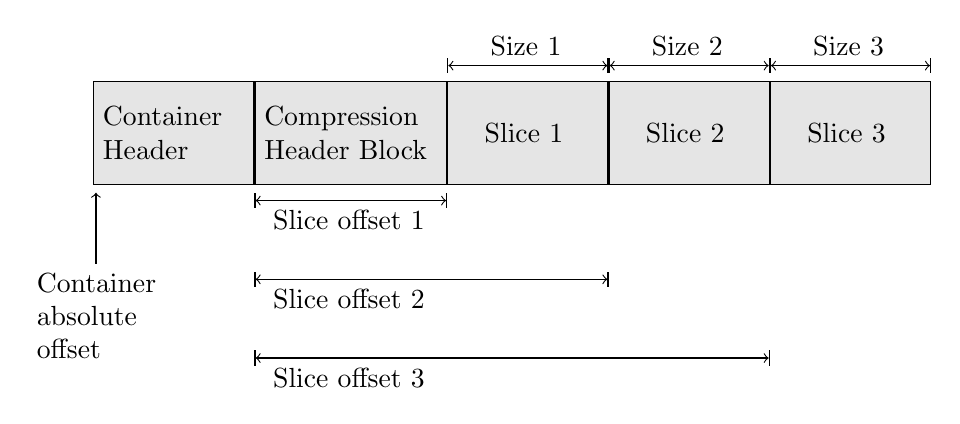
\begin{tikzpicture}[
  boxed/.style={rectangle, draw=black, fill=black!10, minimum height=1.3cm, text width=1.8cm},
]
\node(A) [boxed]{Container Header};
\node(B) [boxed,right,text width=2.2cm] at (A.east){Compression Header Block};
\node(C) [boxed,right] at (B.east){\quad Slice 1};
\node(D) [boxed,right] at (C.east){\quad Slice 2};
\node(E) [boxed,right] at (D.east){\quad Slice 3};

\draw[<-] (A.south west)+(1pt,-0.1cm) -- +(1pt,-1cm)
     node[below, text width=1.5cm]{Container absolute offset};


\draw[|<->|] ([yshift=-0.2cm]B.south west) node[below,xshift=1.2cm]{Slice offset 1}
    -- ([yshift=-0.2cm]B.south east);
\draw[|<->|] ([yshift=-1.2cm]B.south west) node[below,xshift=1.2cm]{Slice offset 2}
    -- ([yshift=-1.2cm]C.south east);
\draw[|<->|] ([yshift=-2.2cm]B.south west) node[below,xshift=1.2cm]{Slice offset 3}
    -- ([yshift=-2.2cm]D.south east);

\draw[|<->|] ([yshift=+0.2cm]C.north west) node[above,xshift=1cm]{Size 1} -- ([yshift=+0.2cm]C.north east);
\draw[|<->|] ([yshift=+0.2cm]D.north west) node[above,xshift=1cm]{Size 2} -- ([yshift=+0.2cm]D.north east);
\draw[|<->|] ([yshift=+0.2cm]E.north west) node[above,xshift=1cm]{Size 3} -- ([yshift=+0.2cm]E.north east);


\end{tikzpicture}
\end{center}

\subsubsection*{BAM index}

BAM indexes are supported by using 4-byte integer pointers called landmarks that 
are stored in container header. BAM index pointer is a 64-bit value with 48 bits 
reserved for the BAM block start position and 16 bits reserved for the in-block 
offset. When used to index CRAM files, the first 48 bits are used to store the 
CRAM container start position and the last 16 bits are used to store the index 
of the landmark in the landmark array stored in  container header. The landmark 
index can be used to access the appropriate slice. 

The above indexing scheme treats CRAM slices as individual records in BAM file. 
This allows to apply BAM indexing to CRAM files, however it introduces some overhead 
in seeking specific alignment start because all preceding records in the slice 
must be read and discarded.

\section{Encodings}
\label{sec:encodings}

% FIXME: we have a mishash of coding, encoding and codec.  We should
% go through the entire document and be consistent.

\subsection{Introduction}

The basic idea for encodings is to efficiently represent byte and integer values.
This can be achieved in a number of ways that most frequently involve some knowledge 
about the nature of the values being encoded, for example, distribution statistics. 
The methods for choosing the best encoding and determining its parameters are very 
diverse and are not part of the CRAM format specification, which only describes 
how the information needed to decode the values should be stored.

\subsection{BYTE}

This encoding simply stores byte values verbatim to a block with a given ID.

\subsubsection*{Parameters}

CRAM format defines the following parameters for BYTE encoding: 

\begin{tabular}{|>{\raggedright}p{100pt}|>{\raggedright}p{100pt}|>{\raggedright}p{230pt}|}
\hline
\textbf{Data type} & \textbf{Name} & \textbf{Comment}
\tabularnewline
\hline
uint7 & id & id of a block containing the byte stream\tabularnewline
\hline
\end{tabular}

\subsection{VARINT\_UNSIGNED}

This encoding stores unsigned integer values using the Variable Length Quantity
format (VLQ)\footnote{https://en.wikipedia.org/wiki/Variable-length\_quantity}.

It is not permitted to store any negative values using this encoding.
However given several data series have ranges that have the
possibility of small negative values (such as -1 for Alignment
Position), it is possible to skew the values slightly by adding an
offset prior to encoding.  This provides a mechanism for guaranteeing
all values remain positive.

Note this offset is added to the value after that value has been
decoded so to encode -1 we may wish to set offset to -1 and encode a
zero.  This mechanism may also be used to skew a range of values that
do not cluster around zero.  For example if a data series has values
ranging from 1000 to 1200, then setting offset to 1000 and encoding
values between 0 and 200 would provide a smaller data footprint.

For data series that require a broader scope of signed values we would
recommend using VARINT\_SIGNED instead.

\subsubsection*{Parameters}

CRAM format defines the following parameters for VARINT\_UNSIGNED encoding: 

\begin{tabular}{|>{\raggedright}p{100pt}|>{\raggedright}p{100pt}|>{\raggedright}p{230pt}|}
\hline
\textbf{Data type} & \textbf{Name} & \textbf{Comment}
\tabularnewline
\hline
sint7 & offset & amount to add to decoded values\tabularnewline
\hline
uint7 & id & id of a block containing the byte stream\tabularnewline
\hline
\end{tabular}

\subsection{VARINT\_SIGNED}

This encoding permits storing a broad range of both positive and
negative values while still following the property of low magnitude
values taking up less space than large magnitude ones.

It achieves this by using ZigZag encoding where signed values 0, -1,
+1, -2, +2 and so on are mapped to unsigned values 0, 1, 2, 3, 4.
These unsigned values are then stored using the same VLQ system used
by VARINT\_UNSIGNED.

As with VARINT\_UNSIGNED, an offset is added to the value after it has
been VLQ and ZigZag decoded.  Combined these permit efficient storage
of a distribution of values centred around a mean.  For example if
the distribution of values in a data series ranged from 1000 to 2000
with a peak at 1500, we could set offset to 1500 and encode values
-500 to +500.

\subsubsection*{Parameters}

CRAM format defines the following parameters for VARINT\_SIGNED encoding: 

\begin{tabular}{|>{\raggedright}p{100pt}|>{\raggedright}p{100pt}|>{\raggedright}p{230pt}|}
\hline
\textbf{Data type} & \textbf{Name} & \textbf{Comment}
\tabularnewline
\hline
sint7 & offset & amount to add to decoded values\tabularnewline
\hline
uint7 & id & id of a block containing the byte stream\tabularnewline
\hline
\end{tabular}


\subsection{CONST\_BYTE}

Sometimes a data series has a constant value throughout the
container.  In this case we can record this value in the Container
Compression Header and avoid the need to store the data series.

\subsubsection*{Parameters}

CRAM format defines the following parameters for CONST\_BYTE encoding: 

\begin{tabular}{|>{\raggedright}p{100pt}|>{\raggedright}p{100pt}|>{\raggedright}p{230pt}|}
\hline
\textbf{Data type} & \textbf{Name} & \textbf{Comment}
\tabularnewline
\hline
byte & value & the constant value\tabularnewline
\hline
\end{tabular}

\subsection{CONST\_INT}

As per CONST\_BYTE, but the value is a signed integer encoded with
VLQ and ZigZag methods.
The overhead of using ZigZag encoding on a constant unsigned value is
an average of 1 bit per container per use of this encoding.

\subsubsection*{Parameters}

CRAM format defines the following parameters for CONST\_INT encoding: 

\begin{tabular}{|>{\raggedright}p{100pt}|>{\raggedright}p{100pt}|>{\raggedright}p{230pt}|}
\hline
\textbf{Data type} & \textbf{Name} & \textbf{Comment}
\tabularnewline
\hline
sint & value & the constant value\tabularnewline
\hline
\end{tabular}

\subsection{BYTE\_ARRAY\_LEN (ID 4)}

Can encode types \textit{Byte[]}.

Often there is a need to encode an array of bytes where the length is
not predetermined.  For example the read identifiers differ per
alignment record, possibly with different lengths, and this length
must be stored somewhere.   Note in contrast to this, quality values
are known to be the same length as the sequence which is an already
known quantity, so the CRAM record encodes this using an implicit
array by asking for multiple values to be decoded rather than using an
explicit byte array encoding.

With BYTE\_ARRAY\_LEN the length is explicitly encoded via its own
sub-encoding prior to the array of bytes itself, also via its own
sub-encoding.

Note these sub-encodings may store the data in the same block, in
which case the length comes first. Alternatively we may decide that
the lengths have their own unique distribution which differs
substantially to the data itself and so should be stored in a
different block to permit better compression.  Having decoded the
length, the decoder must then call the value sub-encoding that many
times to retrieve the bytes.

Given the recursion used here of an encoding using two sub-encodings,
the byte stream for BYTE\_ARRAY\_LEN is the concatenation of both
sub-encodings.

\subsubsection*{Parameters}

The parameters for BYTE\_ARRAY\_LEN are listed below:

\begin{tabular}{|>{\raggedright}p{100pt}|>{\raggedright}p{100pt}|>{\raggedright}p{230pt}|}
\hline
\textbf{Data type} & \textbf{Name} & \textbf{Comment}
\tabularnewline
\hline
encoding\texttt{<}int\texttt{>} & lengths encoding & an encoding describing how 
the arrays lengths are stored\tabularnewline
\hline
encoding\texttt{<}byte\texttt{>} & values encoding & an encoding describing how 
the values (bytes) are stored\tabularnewline
\hline
\end{tabular}

\subsubsection*{Example}

The bytes for an X0:i SAM auxiliary field consisting of 16-bit items
may be written as an X0S tag line.  Despite the size being known, all
tag items are stored as byte arrays, so BYTE\_ARRAY\_LEN is ideal when
coupled with a CONST\_INT encoding to hold the fixed size lengths and
BYTE for the values.

\begin{tabular}{lll}
\hline
\textbf{Bytes} & & \textbf{Meaning}\\
\hline
\texttt{0x04}         & & BYTE\_ARRAY\_LEN encoding ID                                    \\
\texttt{0x07}         & & 7 remaining bytes of BYTE\_ARRAY\_LEN parameters            \\
\\
\texttt{0x44}         & & CONST\_INT encodng ID, for the aux tag lengths \\
\texttt{0x01}         & & remaining length of CONST\_INT encoding \\
\texttt{0x05}         & & length 2 as Zig-Zag format \\
\\
\texttt{0x01}         & & BYTE encoding ID, for the aux tag values \\
\texttt{0x02}         & & 2 more bytes of BYTE parameters                          \\
\texttt{0x81 0x48}    & & uint7 encoding for block ID 200                              \\
\hline
\end{tabular}

\subsection{BYTE\_ARRAY\_STOP (ID 5)}

Can encode types \textit{Byte[]}.

Instead of encoding an explicit length (as per BYTE\_ARRAY\_LEN) this
encoding stores bytes ending in a termination value.  The data
returned should not include this termination byte.  Hence this is
comparable to the C language string encoding, which uses a nul
character for termination, while BYTE\_ARRAY\_LEN is more similar to
the Pascal language string encoding.

Given this encoding is capturing the length within the same data
stream as the bytes, unlike BYTE\_ARRAY\_LEN this does not require
use of sub-encodings.  This makes it considerably simpler, but it has
redundancy when the stored arrays have constant lengths.

The choice of termination symbol is up to the encoder, but logical
choices may include the nul byte or the tab character as both are
illegal within SAM records.

\begin{tabular}{|>{\raggedright}p{100pt}|>{\raggedright}p{100pt}|>{\raggedright}p{230pt}|}
\hline
\textbf{Data type} & \textbf{Name} & \textbf{Comment}
\tabularnewline
\hline
byte & stop byte & a special byte treated as a delimiter\tabularnewline
\hline
uint7 & block id & id of a block containing the byte stream\tabularnewline
\hline
\end{tabular}

% \subsection{Beta coding: codec ID 6}
% 
% Can encode types \textit{Integer}.
% 
% \subsubsection*{Definition}
% 
% Beta coding is a most common way to represent numbers in \emph{binary notation} and is sometimes referred to as binary coding.
% The decoder reads the specified fixed number of bits (most significant first) and subtracts the offset value to get the decoded integer.
% 
% \subsubsection*{Parameters}
% 
% CRAM format defines the following parameters of beta coding: 
% 
% \begin{tabular}{|>{\raggedright}p{144pt}|>{\raggedright}p{144pt}|>{\raggedright}p{144pt}|}
% \hline
% \textbf{Data type} & \textbf{Name} & \textbf{Comment}\tabularnewline
% \hline
% itf8 & offset & offset is subtracted from each value during decode\tabularnewline
% \hline
% itf8 & length & the number of bits used\tabularnewline
% \hline
% \end{tabular}
% 
% \subsubsection*{Examples}
% 
% If we have integer values in the range 10 to 15 inclusive, the largest value would traditionally need 4 bits, but with an offset of -10 we can hold values 0 to 5, using a fixed size of 3 bits.
% Using fixed Offset and Length coming from the beta parameters, we decode these values as:
% 
% \begin{tabular}{|>{\raggedright}p{105pt}|>{\raggedright}p{105pt}|>{\raggedright}p{105pt}|>{\raggedright}p{105pt}|}
% \hline
% Offset & Length & \textbf{Bits} & \textbf{Value}\tabularnewline
% \hline
% -10 & 3 & 000 & 10\tabularnewline
% \hline
% -10 & 3 & 001 & 11\tabularnewline
% \hline
% -10 & 3 & 010 & 12\tabularnewline
% \hline
% -10 & 3 & 011 & 13\tabularnewline
% \hline
% -10 & 3 & 100 & 14\tabularnewline
% \hline
% -10 & 3 & 101 & 15\tabularnewline
% \hline
% \end{tabular}
% 
% \subsection{Subexponential coding: codec ID 7}
% 
% Can encode types \textit{Integer}.
% 
% \subsubsection*{Definition}
% 
% Subexponential coding\footnote{Fast progressive lossless image compression, Paul G. Howard and Jeffrey Scott Vitter, 1994. \url{http://www.ittc.ku.edu/~jsv/Papers/HoV94.progressive_FELICS.pdf}} is parametrized by a non-negative integer $k$.
% For values $n < 2^{k+1}$ subexponential coding produces codewords identical to Rice coding \footnote{\url{https://en.wikipedia.org/wiki/Golomb_coding\#Rice_coding}}.  For larger values it grows logarithmically with $n$.
% 
% \subsubsection*{Encoding}
% 
% \begin{enumerate}
% \item Add $\mathit{offset}$ to $n$.
% 
% \item Determine $u$ and $b$ values from $n$
% \begin{align*}
% b =
% \begin{cases}
%   \ k                        & \text{ if $n < 2^k$} \\
%   \ \lfloor log_{2}n \rfloor & \text{ if $n \ge 2^k$}
% \end{cases}
% &\
% &u =
% \begin{cases}
%   \ 0     & \text{ if $n < 2^k$} \\
%   \ b-k+1 & \text{ if $n \ge 2^k$}
% \end{cases}
% \end{align*}
% 
% \item Write $u$ in unary form; $u$ 1 bits followed by a single 0 bit.
% 
% \item Write the bottom $b$-bits of $n$ in binary form.
% \end{enumerate}
% 
% \subsubsection*{Decoding}
% 
% \begin{enumerate}
% \item Read $u$ in unary form, counting the number of leading 1s (prefix) in the codeword (discard the trailing 0 bit).
% 
% \item Determine $n$ via:
% \begin{enumerate}
% \item if $u = 0$ then read $n$ as a $k$-bit binary number.
% \item if $u \ge 1$ then read $x$ as a $(u + k - 1)$-bit binary. Let $n = 2^{u+k-1} + x$.
% \end{enumerate}
% 
% \item Subtract $\mathit{offset}$ from $n$.
% \end{enumerate}
% 
% \subsubsection*{Examples}
% 
% \begin{tabular}{|>{\raggedright}p{105pt}|>{\raggedright}p{105pt}|>{\raggedright}p{105pt}|>{\raggedright}p{105pt}|}
% \hline
% \textbf{Number} & \textbf{Codeword, k=0} & \textbf{Codeword, k=1} & \textbf{Codeword, 
% k=2}\tabularnewline
% \hline
% 0 & 0 & 00 & 000\tabularnewline
% \hline
% 1 & 10 & 01 & 001\tabularnewline
% \hline
% 2 & 1100 & 100 & 010\tabularnewline
% \hline
% 3 & 1101 & 101 & 011\tabularnewline
% \hline
% 4 & 111000 & 11000 & 1000\tabularnewline
% \hline
% 5 & 111001 & 11001 & 1001\tabularnewline
% \hline
% 6 & 111010 & 11010 & 1010\tabularnewline
% \hline
% 7 & 111011 & 11011 & 1011\tabularnewline
% \hline
% 8 & 11110000 & 1110000 & 110000\tabularnewline
% \hline
% 9 & 11110001 & 1110001 & 110001\tabularnewline
% \hline
% 10 & 11110010 & 1110010 & 110010\tabularnewline
% \hline
% \end{tabular}
% 
% \subsubsection*{Parameters}
% 
% \begin{tabular}{|>{\raggedright}p{100pt}|>{\raggedright}p{100pt}|>{\raggedright}p{230pt}|}
% \hline
% \textbf{Data type} & \textbf{Name} & \textbf{Comment}
% \tabularnewline
% \hline
% itf8 & offset & offset is subtracted from each value during decode\tabularnewline
% \hline
% itf8 & k & the order of the subexponential coding\tabularnewline
% \hline
% \end{tabular}
% 
% \subsection{Gamma coding: codec ID 9}
% 
% Can encode types \textit{Integer}.
% 
% \subsubsection*{Definition}
% 
% \emph{Elias gamma code} is a prefix encoding of positive integers. This is a combination 
% of unary coding and beta coding. The first is used to capture the number of bits 
% required for beta coding to capture the value. 
% 
% \subsubsection*{Encoding}
% 
% \begin{enumerate}
% \item Write it in binary.
% 
% \item Subtract $1$ from the number of bits written in step 1 and prepend that many zeros.
% 
% \item An equivalent way to express the same process:
% 
% \item Separate the integer into the highest power of $2$ it contains ($2N$) and the remaining 
% $N$ binary digits of the integer.
% 
% \item Encode $N$ in unary; that is, as $N$ zeroes followed by a one.
% 
% \item Append the remaining $N$ binary digits to this representation of $N$.
% \end{enumerate}
% 
% \subsubsection*{Decoding}
% 
% \begin{enumerate}
% \item Read and count 0s from the stream until you reach the first 1. Call this count 
% of zeroes $N$.
% 
% \item Considering the one that was reached to be the first digit of the integer, with 
% a value of $2N$, read the remaining $N$ digits of the integer.
% \end{enumerate}
% 
% \subsubsection*{Examples}
% 
% \begin{tabular}{|>{\raggedright}p{76pt}|>{\raggedright}p{107pt}|}
% \hline
% \textbf{Value} & \textbf{Codeword}\tabularnewline
% \hline
% 1 & 1\tabularnewline
% \hline
% 2 & 010\tabularnewline
% \hline
% 3 & 011\tabularnewline
% \hline
% 4 & 00100\tabularnewline
% \hline
% \end{tabular}
% 
% \subsubsection*{Parameters}
% 
% \begin{tabular}{|>{\raggedright}p{144pt}|>{\raggedright}p{144pt}|>{\raggedright}p{144pt}|}
% \hline
% \textbf{Data type} & \textbf{Name} & \textbf{Comment}\tabularnewline
% \hline
% itf8 & offset & offset to subtract from each value after decode\tabularnewline
% \hline
% \end{tabular}
% 
% \subsection{DEPRECATED: Golomb coding: codec ID 2}
% 
% Can encode types \textit{Integer}.
% 
% Note this codec has not been used in any known CRAM implementation since before CRAM v1.0.
% Nor is it implemented in some of the major software.
% Therefore its use is not recommended.
% 
% \subsubsection*{Definition}
% 
% \emph{Golomb encoding} is a prefix encoding optimal for representation of random 
% positive numbers following geometric distribution. 
% 
% \subsubsection*{Encoding}
% 
% \begin{enumerate}
% \item Fix the parameter $M$ to an integer value.
% 
% \item For $N$, the number to be encoded, find
% 
% \begin{enumerate}
% \item quotient $q = \lfloor N/M \rfloor$
% 
% \item remainder $r = N \bmod M$
% \end{enumerate}
% 
% \item Generate Codeword
% 
% \begin{enumerate}
% \item The Code format : \texttt{<}Quotient Code\texttt{>}\texttt{<}Remainder Code\texttt{>}, 
% where
% 
% \item Quotient Code (in unary coding)
% 
% \begin{enumerate}
% \item Write a $q$-length string of 1 bits
% 
% \item Write a 0 bit
% \end{enumerate}
% 
% \item Remainder Code (in truncated binary encoding)
% 
% Set $b=\lceil log_{2}(M) \rceil$
% 
% \begin{enumerate}
% \item If $r < 2^{b}-M$ code $r$ as plain binary using $b-1$ bits.
% 
% \item If $r \ge 2^{b}-M$ code the number $r+2^{b}-M$ in plain binary representation 
% using $b$ bits.
% \end{enumerate}
% \end{enumerate}
% \end{enumerate}
% 
% \subsubsection*{Decoding}
% 
% \begin{enumerate}
% \item Read $q$ via unary coding: count the number of 1 bits and consume the following 0 bits.
% \item Set $b=\lceil log_{2}(M) \rceil$
% \item Read $r$ via $b-1$ bits of binary coding
% \item If $r \ge 2^{b}-M$
% \begin{enumerate}
% \item Read 1 single bit, $x$.
% \item Set $r = r*2 + x - (2^{b}-M)$
% \end{enumerate}
% \item Value is $q*M + r - \mathit{offset}$
% \end{enumerate}
% 
% \subsubsection*{Examples}
% 
% \begin{tabular}{|>{\raggedright}p{76pt}|>{\raggedright}p{107pt}|}
% \hline
% \textbf{Number} & \textbf{Codeword, M=10, (thus b=4)}\tabularnewline
% \hline
% 0 & 0000\tabularnewline
% \hline
% 4 & 0100\tabularnewline
% \hline
% 10 & 10000\tabularnewline
% \hline
% 26 & 1101100\tabularnewline
% \hline
% 42 & 11110010\tabularnewline
% \hline
% \end{tabular}
% 
% \subsubsection*{Parameters}
% 
% Golomb coding takes the following parameters: 
% 
% \begin{tabular}{|>{\raggedright}p{144pt}|>{\raggedright}p{144pt}|>{\raggedright}p{144pt}|}
% \hline
% \textbf{Data type} & \textbf{Name} & \textbf{Comment}\tabularnewline
% \hline
% itf8 & offset & offset is added to each value\tabularnewline
% \hline
% itf8 & M & the golomb parameter (number of bins)\tabularnewline
% \hline
% \end{tabular}
% 
% \subsection{DEPRECATED: Golomb-Rice coding: codec ID 8}
% 
% Can encode types \textit{Integer}.
% 
% Note this codec has not been used in any known CRAM implementation since before CRAM v1.0.
% Nor is it implemented in some of the major software.
% Therefore its use is not recommended.
% 
% Golomb-Rice coding is a special case of Golomb coding when the M parameter is a power of 2.
% The reason for this coding is that the division operations in Golomb coding can be replaced with bit shift operators as well as avoiding the extra $r < 2^{b}-M$ check.

\section{Block compression methods}

Each block will hold different types of data and may have very
different characteristics for compression.  Hence CRAM can utilise
several different compression methods. Each method has an associated numeric code which is defined in Section~\ref{sec:block-struct}.

The following methods are defined.
Exact definitions of these methods are in their respective internet links or the ancillary \textit{CRAMcodecs} document found along side this specification.

\subsection{Gzip}

The Gzip specification is defined in RFC 1952.
Gzip in turn is an encapsulation on the Deflate algorithm defined in RFC 1951.

\subsection{Bzip2}

First available in CRAM v2.0.

Bzip2 is a compression method utilising the Burrows Wheeler Transform, Move To Front transform, Run Length Encoding and a Huffman entropy encoder. 
It is often superior to Gzip for textual data.

An informal format specification exists:\\
\url{https://github.com/dsnet/compress/blob/master/doc/bzip2-format.pdf}

\subsection{LZMA}

First available in CRAM v3.0.

LZMA is the Lempel-Ziv Markov chain algorithm.
CRAM uses the xz Stream format to encapsulate this algorithm, as defined in \url{https://tukaani.org/xz/xz-file-format.txt}.

\subsection{rANS4x8 codec}

First available in CRAM v3.0.

rANS is the range-coder variant of the Asymmetric Numerical
System\footnote{J. Duda, \textit{Asymmetric numeral systems: entropy
    coding combining speed of Huffman coding with compression rate of
    arithmetic coding}, \url{http://arxiv.org/abs/1311.2540}}.

``4x8'' refers to 4-way interleaving with 8-bit renormalisation.\newline
This variant of rANS first appeared in CRAM v3.0.

Details of this algorithm have been moved to the \textit{CRAMcodecs} document.

\subsection{rANS4x16 codec}

First available in CRAM v3.1.

``4x16'' refers to 4-way interleaving with 16-bit renormalisation.\newline
This variant of rANS first appeared in CRAM v3.1.

Details of this algorithm are listed in the \textit{CRAMcodecs} document.

\subsection{adaptive arithemtic coding}

First available in CRAM v3.1.

An entropy encoder that is slower but slightly more concise than
rANS.  It achieves this by adapting the probabilities as it compresses
and decompresses instead of using a fixed table.

Details of this algorithm are listed in the \textit{CRAMcodecs} document.

\subsection{fqzcomp codec}

First available in CRAM v3.1.

This is a method dedicated to compression of quality values.

Details of this algorithm are listed in the \textit{CRAMcodecs} document.

\subsection{name tokeniser}

First available in CRAM v3.1.

This is a method dedicated to compression of read names.

Details of this algorithm are listed in the \textit{CRAMcodecs} document.

\appendix
\renewcommand{\thesection}{\arabic{section}}

\newcommand{\appsection}[1]{%
  \addtocounter{section}{1}
  \section*{Appendix~\thesection \quad #1}
  \addcontentsline{toc}{section}{Appendix~\thesection \quad #1}
}

\appsection{Choosing the container size}

The CRAM format does not constrain the size of the containers.
However, the following should be considered when deciding the container size:

-- Data can be compressed better by using larger containers.

-- Random access performance is better for smaller containers.

-- Streaming is more convenient for small containers.

-- Applications typically buffer containers into memory.

-- Multi-threaded applications likely have a granularity of 1
container for each unit of work.

As a guidance, the default container size for htslib and htsjdk is one
slice of 10,000 short reads (fewer for long reads), but some users
find 1,000 is more appropriate if they need a lot of random access.

\appsection{CRAM 4.0 changes and rationale}
\label{sec:cram4changes}

CRAM 4.0 has a number of changes.  For those familier with the version
3.0 format, this is a list of changes along with a rationale for
making them.

\begin{description}
\item[New variable sized integer encoding]\ \newline
  Use VLQ (https://en.wikipedia.org/wiki/Variable-length\_quantity)
  instead of ITF8 and LTF8.

  This has the impact of not needing to distinguish between 32-bit and
  64-bit quantities, which we previously needed to do with ITF8 vs
  LTF8.  It also has a small reduction to compressed sizes.


\item[Long chromosome support]\ \newline
  A corollary of the removal of ITF8 and LTF8 means all fields
  can now be 64-bit if appropriate.  Importantly this removes the
  32-bit limit on the size of AP (alignment pos), TS (template size),
  NP (next mate pos).


\item[Signed numbers]\ \newline
  Variable sized integer encoding can now also do signed numbers.
  Previously -1 was stored as FF FF FF 0F (ITF8) and even more FFs
  for LTF8.  This is unwieldy and also bakes in knowledge of the
  size of the intended data type, making it impossible to increase
  data type sizes without changing the format.

  Signed fields are used for AP (alignment pos), TS (template size)
  and RG (read group, which can be -1 for not present).


\item[MD, NM presence and location]\ \newline
  CRAM derives MD and NM tags on-the-fly where possible.  However it
  doesn't record whether they were in the original data.

  The presence of MD and NM are now recorded, so if the input data didn't
  have them we won't reproduce on decode, and vice versa.  The
  location of MD, NM and RG in the tag stream are now also recorded,
  meaning CRAM 4.0 will round-trip more precisely.


\item[Quality value orientation]\ \newline
  On some technologies it is better to record qualities in their
  original orientation rather than the alignment orientation as this
  improves compression ratios.

  This is an optional setting in the compression header.  The data
  should be automatically flipped back during decode so the operation
  is transparent to the user.


\item[New CF explicit template size flag]\ \newline
  In CRAM RNEXT, PNEXT and TLEN are generated on-the-fly for read
  pairs residing in the same slice.  If we wish to preserve data
  verbatim for exceptions, such as TLEN off-by-one errors (common in
  old data) or TLEN 5' to 5' vs leftmost to rightmost differences then
  we had to mark the record as ``detached'' and store all 3 fields.

  We now have an flag to state that TLEN is explicitly stored without
  needing to use the CF detached flag.  This can have a substantial
  impact on file sizes for some older data sets.


\item[Deduplication of read names]\ \newline
  For read pairs residing in the same slice we can use the same logic
  we previously used for RNEXT, PNEXT and TLEN generation to also
  deduplicate read names so it only needs storing once.

  This roughly halves the size of uncompressed RN data series,
  reducing the compressed size.

{\color{gray}
\item[(For consideration) Removal of slices]\ \newline
  CRAM 3.0 offers the ability to have multiple slices per container.
  
  This is largely unused and does not provide the originally planned
  benefits of sharing compression meta-data between slices.  The
  defaults from both htslib and htsjdk are one slice per container.

  Removal of multi-slice containers, and by extension slices
  themselves, offers a simplified interface.

  An alternative to this is to permit another set of blocks prior to
  the first slice, with duplicate block IDs to those used in the
  slices.  These blocks pertain to the container and are utilised in
  unison with the per slice blocks.  For rANS they could hold the
  frequency tables, permitting this to be shared across slices.  For
  gzip or zstd they could hold a predefined dictionary, permitting
  more efficient compression of small blocks.  This may grant finer
  grained random access capability without suffering so much data
  expansion.
}

\item[TODO: add PACK, RLE and DELTA encodings]\ \newline

\item[TODO: sanitize read\_names\_included]\ \newline
  Given we now state a blank name will copy from the mate pair and
  auto-generate if not, there's no need for this field.  We can just
  store blank names and cull the whole RN in DecodeMateData vs in-line
  shenanigans.

\item[TODO: make all aux tags first class encoding objects]\ \newline
  Right now aux tags are basically byte arrays encoded as per BAM.
  This isn't so efficient.  For example an XX:S data series with
  values ranging 0 to 500 but with many more small values are a few
  large ones would be better encoded as VLQ than an array of 16-bit
  quantities.

\end{description}

\end{document}

\title{CRAM format specification (version 4.0)}
\author{samtools-devel@lists.sourceforge.net}
\date{\headdate}
\maketitle


\begin{quote}\small
The master version of this document can be found at
\url{https://github.com/samtools/hts-specs}.\\
This printing is version~\commitdesc\ from that repository,
last modified on the date shown above.
\end{quote}

\begin{center}
\textit{license: Apache 2.0}
\end{center}
\vspace*{1em}

\tableofcontents
\newpage

\section{Overview}

This specification describes the CRAM 4.0 format. 

CRAM has the following major objectives:

\begin{enumerate}
\item Significantly better lossless compression than BAM

\item Full compatibility with BAM

\item Effortless transition to CRAM from using BAM files

\item Support for controlled loss of BAM data
\end{enumerate}

The first three objectives allow users to take immediate advantage of the CRAM 
format while offering a smooth transition path from using BAM files. The fourth 
objective supports the exploration of different lossy compression strategies and 
provides a framework in which to effect these choices. Please note that the CRAM 
format does not impose any rules about what data should or should not be preserved. 

Data in CRAM is aggregated by data type (analogous to SAM columns)
known as Data Series and stored in blocks with each block compressed
using a choice of general purpose or custom compression codecs.
Sequence is typically encoded relative to a reference
sequence\footnote{Markus Hsi-Yang Fritz, Rasko Leinonen, Guy Cochrane,
  and Ewan Birney, \textbf{Efficient storage of high throughput DNA
    sequencing data using reference-based compression}, {\sl Genome
    Res.}~2011~21: 734--740;
  \href{http://dx.doi.org/doi:10.1101/gr.114819.110}{doi:10.1101/gr.114819.110};
  {\sc pmid:}21245279.}, but this is not a requirement.  Both aligned
and unaligned sequence is supported.

\section{Data types and formats}
\subsection*{Structures}

The CRAM format consists of header structures (container, compression, slice and block) and data series stored within the blocks themselves.
The fields of these structures use a mixture of fundamental types - boolean, byte, integer or array thereof - which are defined below.

% Types used in structures.
% Container:  uint, sint, uint[], byte[4](CRC), byte[]
% Block:      byte, uint, byte[], byte[4](CRC)
% CompHdr:    map, bool, byte[5], uint, byte[], encoding<>
% Slice:      sint, uint, uint[], byte[16], byte[]

\begin{tabular}{lll}
\textbf{Field type}  & \textbf{Format} & \textbf{Description}\\
\textit{bool}  & \textbf{byte} & A boolean, 0 (false) or 1 (true), stored as a byte. \\
\textit{byte}  & \textbf{byte} & An unsigned single byte (8 bits)  \\
\textit{uint}  & \textbf{VLQ\_unsigned} & A variable length integer $x >= 0$\\
\textit{sint}  & \textbf{VLQ\_signed}   & A variable length integer (may be negative)\\
\textit{array\texttt{<}type\texttt{>}} & \textbf{array} & An array of items of \textit{type} including the dimension\\
\\
\textit{type[]}  & \textit{as appropriate} & Zero or more items with unspecified length\\
\textit{type[4]} & \textit{as appropriate} & A constant number of items, dimension not stored\\
\end{tabular}
\vskip 10pt

The on-disk format for each of these encodings is listed below:

\begin{description}
\item[\textbf{byte}]\ \newline
A single byte

\item[\textbf{VLQ\_unsigned}]\ \newline
Integer values are encoded using Variable Length
Quantity\footnote{\url{https://en.wikipedia.org/wiki/Variable-length_quantity}}.

If the value is larger than 7-bits then the top-bit of the byte is
set, indicating a subsequent byte must be read.  This is repeated
until the top bit is unset. Bytes are written with the most
significant values first (big-endian format), which simplifies the
decode process.

Algorithmically this looks like:

\begin{algorithmic}[1]
\Statex
\Statex \textit{Read a variable sized unsigned integer 7-bits at a time.}
\Function{ReadUint7}{}
  \State $value \gets 0$
  \Repeat
    \State $c \gets$ \Call{ReadUint8}{}
    \State $value \gets (value \shiftl 7) + (c \bitand 127)$
  \Until{$c < 128$}
  \State \Return $value$
  \EndFunction
\end{algorithmic}

\item[\textbf{VLQ\_unsigned}]\ \newline
Signed integers are initially transformed to unsigned values using a zig-zag transformation, and then encoded as per unsigned values.
This maps signed values 0, -1, +1, -2, +2 to unsigned values 0, 1, 2, 3, 4 respectively, and vice versa during decode.

The zig-zag encoding method involves shifting the value left 1
bit and then XORing with all-bits-zero if positive or all-bits-one if
negative. I.e. $(v \shiftl 1) \bitxor (v \shiftr 31)$ for a
32-bit quantity using a 2's complement arithmetic shift right.

Decoding a zig-zag value is similar.  We XOR the value shifted right 1
bit with 0 or -1, taken from the negation of the bottom bit, as seen
below.

\begin{algorithmic}[1]
\Statex
\Statex \textit{Read a variable sized signed integer 7-bits at a time.}
\Function{ReadSint7}{}
  \State $value \gets $ \Call{ReadUint7}{}
  \State \Return $(value \shiftr 1) \bitxor -(value \bitand 1)$
  \EndFunction
\end{algorithmic}

\item[\textbf{array}]\ \newline
An array of items with the array dimension explicitly stored.
The array dimension is first, using VLQ\_signed format, followed by the array elements stored as per their \textit{type}.

\end{description}

Other custom data types exist, but will be introduced in the relevant sections.

\section{File Layout}

The basic structure of a CRAM file is a file header (magic number)
followed by a series of containers.  The first of these containers
holds textual meta-data (CRAM Header Container) and the last is used
as an end-of-file marker (CRAM EOF Container) with everyone inbetween
holding the sequence records themselves (Data Contaners).

\begin{center}
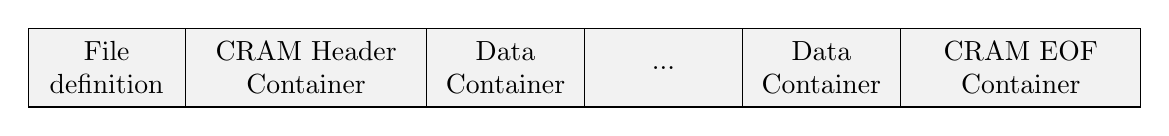
\begin{tikzpicture}[
  every node/.style={scale=1.0},
  boxes/.style={rectangle split,rectangle split parts=#1,draw,rectangle split horizontal,text width=5em,align=center,minimum height=1cm,fill=black!5,on grid},
  notes/.style={text width=20em,align=center,minimum height=1cm,on grid},
]
\node (file) [boxes=6] {
\nodepart{one}File definition
\nodepart[text width=8em]{two}CRAM Header Container
\nodepart{three}Data Container
\nodepart{four}...
\nodepart{five}Data Container
\nodepart[text width=8em]{six}CRAM EOF Container
};
\end{tikzpicture}

Figure 1: A CRAM file consists of a file definition, followed by a header container, then other containers.
\end{center}

Containers are just a Container Header Structure followed by one or
more Blocks.  Blocks have different types (see
~\ref{subsec:block-content-types}) corresponding to their usage.
Note the block itself also consists of a defined structure followed by
the block contents data.

\begin{center}
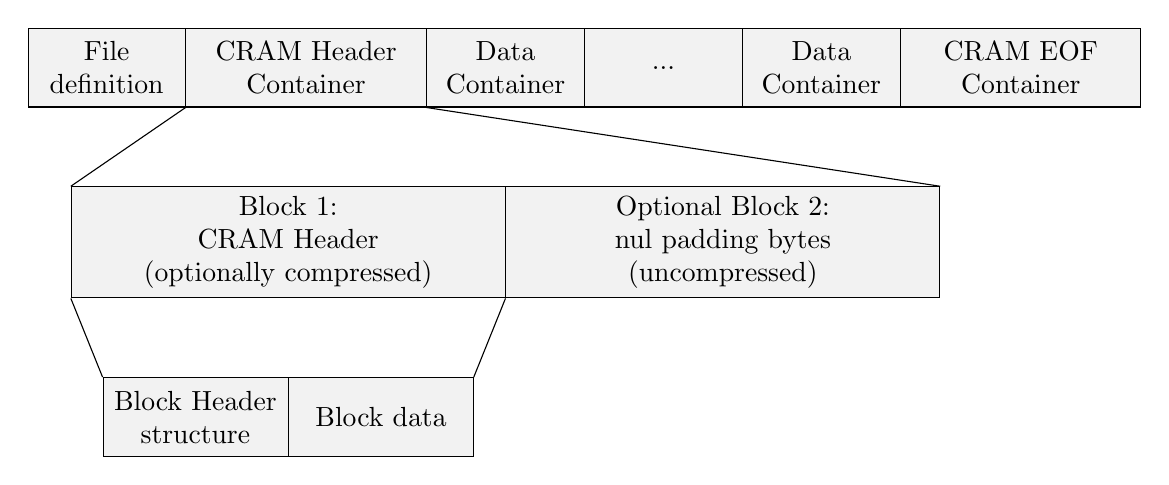
\begin{tikzpicture}[
  every node/.style={scale=1.0},
  boxes/.style={rectangle split,rectangle split parts=#1,draw,rectangle split horizontal,text width=5em,align=center,minimum height=1cm,fill=black!5,on grid},
  notes/.style={text width=20em,align=center,minimum height=1cm,on grid},
]
\node (file) [boxes=6] {
\nodepart{one}File definition
\nodepart[text width=8em]{two}CRAM Header Container
\nodepart{three}Data Container
\nodepart{four}...
\nodepart{five}Data Container
\nodepart[text width=8em]{six}CRAM EOF Container
};

\node (header) [boxes=2,below=1 of file.three south, text width=15em] {
\nodepart{one}Block 1:\break
CRAM Header\break
(optionally compressed)
\nodepart{two}Optional Block 2:\break
nul padding bytes\break
(uncompressed)
};
\draw (file.one split south) to (header.north west);
\draw (file.two split south) to (header.north east);

\node (blocks) [boxes=2,below=1 of header.one south,text width=6em] {
\nodepart{one}Block Header structure
\nodepart{two}Block data
};
\draw (header.south west) to (blocks.north west);
\draw (header.two split south) to (blocks.north east);
\end{tikzpicture}

Figure 2: The the first container holds the CRAM header text.
\end{center}

The first container, called the CRAM header container, is used to
store a textual header as described in the SAM specification (see the
section 7.1).  This is optionally followed by another uncompressed
block of nul padding bytes.  The purpose of this additional block is
to permit in-situ modification of the CRAM header without the
requirement to rewrite the entire file (instead needing just this
container to be rewritten, provided it can be padded to an identical
size).

\begin{center}
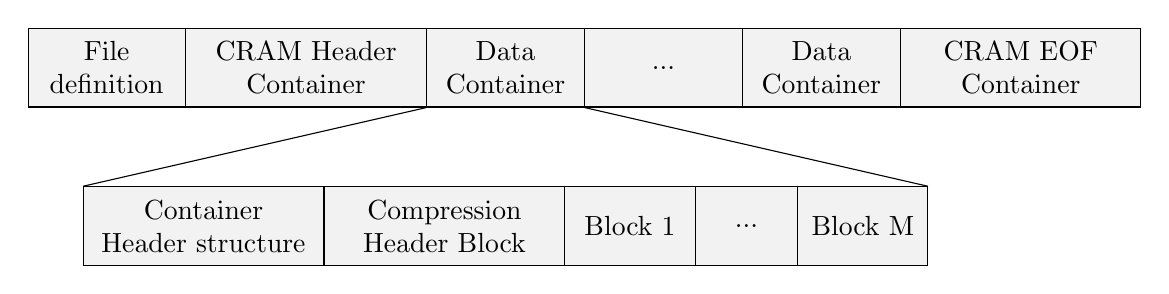
\begin{tikzpicture}[
  every node/.style={scale=1.0},
  boxes/.style={rectangle split,rectangle split parts=#1,draw,rectangle split horizontal,text width=5em,align=center,minimum height=1cm,fill=black!5,on grid},
  notes/.style={text width=20em,align=center,minimum height=1cm,on grid},
]
\node (file) [boxes=6] {
\nodepart{one}File definition
\nodepart[text width=8em]{two}CRAM Header Container
\nodepart{three}Data Container
\nodepart{four}...
\nodepart{five}Data Container
\nodepart[text width=8em]{six}CRAM EOF Container
};

\node (container) [boxes=5,below=1 of file.three south,text width=8em] {
\nodepart{one}Container Header structure
\nodepart{two}Compression Header Block
\nodepart[text width=4em]{three}Block 1
\nodepart[text width=3em]{four}...
\nodepart[text width=4em]{five}Block M
};
\draw (file.two split south) to (container.north west);
\draw (file.three split south) to (container.north east);
\end{tikzpicture}

Figure 3: Containers as a series of blocks
\end{center}

The Data Containers hold the sequence records themselves.
These start with a Compression Header block which holds meta-data
describing how and where the Data Series are encoded within this
container.

\begin{center}
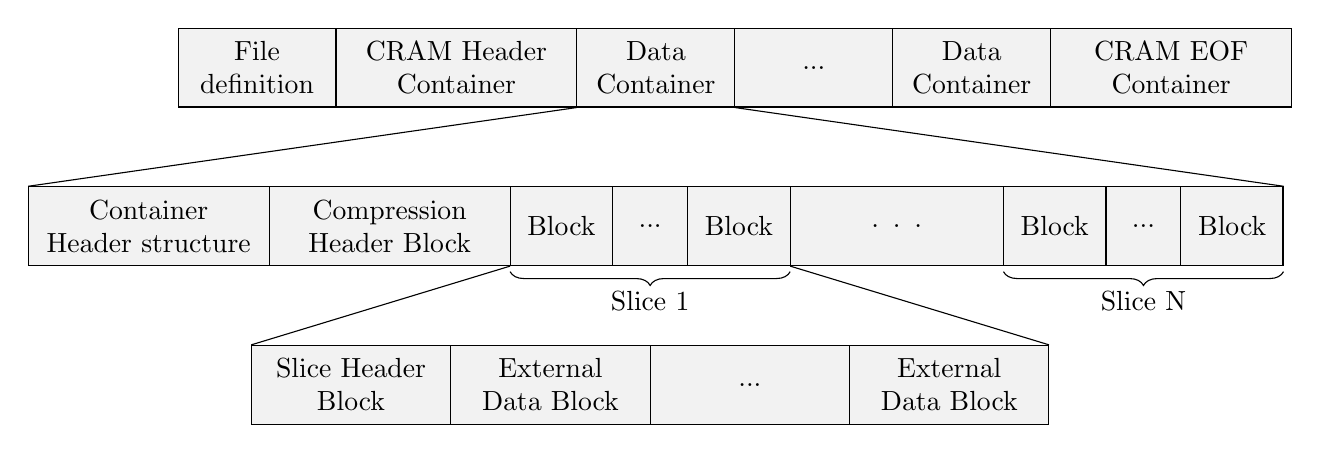
\begin{tikzpicture}[
  every node/.style={scale=1.0},
  boxes/.style={rectangle split,rectangle split parts=#1,draw,rectangle split horizontal,text width=5em,align=center,minimum height=1cm,fill=black!5,on grid},
  notes/.style={text width=20em,align=center,minimum height=1cm,on grid},
]
\node (file) [boxes=6] {
\nodepart{one}File definition
\nodepart[text width=8em]{two}CRAM Header Container
\nodepart{three}Data Container
\nodepart{four}...
\nodepart{five}Data Container
\nodepart[text width=8em]{six}CRAM EOF Container
};

\node (container) [boxes=9,below=1 of file.three south,text width=8em] {
\nodepart{one}Container Header structure
\nodepart{two}Compression Header Block
\nodepart[text width=3em]{three}Block
\nodepart[text width=2em]{four}...
\nodepart[text width=3em]{five}Block
\nodepart[text width=7em]{six}. . .
\nodepart[text width=3em]{seven}Block
\nodepart[text width=2em]{eight}...
\nodepart[text width=3em]{nine}Block
};
\draw (file.two split south) to (container.north west);
\draw (file.three split south) to (container.north east);

\draw[decoration={brace,mirror,amplitude=5pt,raise=2pt},decorate]
  (container.two split south) to (container.five split south);
\node [below=0.2 of container.four south] {Slice 1};

\draw[decoration={brace,mirror,amplitude=5pt,raise=2pt},decorate]
  (container.six split south) to (container.south east);
\node [below=0.2 of container.eight south] {Slice N};

\node (slice) [boxes=4,below=1 of container.four south, text width=6.5em] {
\nodepart{one}Slice Header Block
\nodepart{two}External Data Block
\nodepart{three}...
\nodepart{four}External Data Block
};
\draw (container.two split south) to (slice.north west);
\draw (container.five split south) to (slice.north east);
\end{tikzpicture}

Figure 4: Slices formed from a series of concatenated blocks
\end{center}

The blocks after the compression header are organised logically into slices. One 
slice may contain, for example, a contiguous region of alignment data. Slices begin 
with a slice header block and are followed by one or more data blocks.
It is these data blocks which hold the primary bulk of CRAM data, the
Data Series.

Note many CRAM files will just use one slice per contaner as this is
the default output format of several major implementations.

\subsection{File definition}

Each CRAM file starts with a fixed length (26 bytes) definition with the following 
fields:

\begin{tabular}{|l|l|l|}
\hline
\textbf{Data type} & \textbf{Name} & \textbf{Value}\tabularnewline
\hline
byte[4] & format magic number & CRAM (0x43 0x52 0x41 0x4d)\tabularnewline
\hline
byte & major format number & 3 (0x3)\tabularnewline
\hline
byte & minor format number & 1 (0x1)\tabularnewline
\hline
byte[20] & file id & CRAM file identifier (e.g. file name or SHA1 checksum)\tabularnewline
\hline
\end{tabular}

Valid CRAM \textit{major}.\textit{minor} version numbers are as follows:

\begin{itemize}
\item[\textit{1.0}]
The original public CRAM release.

\item[\textit{2.0}]
The first CRAM release implemented in both Java and C; tidied up
implementation vs specification differences in \textit{1.0}.

\item[\textit{2.1}]
Gained end of file markers; compatible with \textit{2.0}.

\item[\textit{3.0}]
Additional compression methods; header and data checksums;
improvements for unsorted data.

\item[\textit{3.1}]
Additional block compression codecs only.

\item[\textit{4.0}]
This specification.  Revised variable sized integers, MD/NM/RG tag
locators, and deduplication of read names.  Removed some encodings.
See \ref{sec:cram4changes} for a more detailed list of changes.
\end {itemize}

CRAM 3.0 and 3.1 differ only in the list of compression
methods available, so tools that output CRAM 3 without using any 3.1
codecs should write the header to indicate 3.0 in order to permit
maximum compatibility.

\subsection{Container header structure}

The file definition is followed by one or more containers with the following header 
structure where the container content is stored in the `blocks' field:

\begin{tabular}{|l|>{\raggedright}p{120pt}|>{\raggedright}p{260pt}|}
\hline
\textbf{Data type} & \textbf{Name} & \textbf{Value}
\tabularnewline
\hline
uint7 & length & the sum of the lengths of all blocks in this container (headers and data);
equal to the total byte length of the container minus the byte length of this header structure\tabularnewline
\hline
int7 & reference sequence id & reference sequence identifier  or\linebreak{}
-1 for unmapped reads\linebreak{}
-2 for multiple reference sequences.\linebreak{}
All slices in this container must have a reference sequence id matching this value.\tabularnewline
\hline
uint7 & starting position on the reference & the alignment start position or\linebreak{}
0 if the container is multiple-reference
or contains unmapped unplaced reads\tabularnewline
\hline
uint7 & alignment span & the length of the alignment or\linebreak{}
0 if the container is multiple-reference
or contains unmapped unplaced reads\tabularnewline
\hline
uint7 & number of records & number of records in the container\tabularnewline
\hline
uint7 & record counter & 1-based sequential index of records in the file/stream.\tabularnewline
\hline
uint7 & bases & number of read bases\tabularnewline
\hline
uint7 & number of blocks & the total number of blocks in this container\tabularnewline
\hline
array<uint7> & landmarks & the locations of slices in this container as byte offsets from the end of 
this container header, used for random access indexing.
The landmark count must equal the slice count.\linebreak{}
Since the block before the first slice is the compression header,
landmarks[0] is equal to the byte length of the compression header.\tabularnewline
\hline
uint32 & crc32 & CRC32 hash of the all the preceding bytes in the container.\tabularnewline
\hline
byte[ ] & blocks & The blocks contained within the container.\tabularnewline
\hline
\end{tabular}

\subsubsection*{CRC32}
This is a cyclic redundancy checksum 32-bit long with the polynomial 0x04C11DB7. Please refer to \href{http://www.itu.int/rec/recommendation.asp?type=folders&lang=e&parent=T-REC-V.42}{ITU-T V.42} for more details. The value of the CRC32 hash function is written as an integer.


\subsection{Block structure}
\label{sec:block-struct}

Containers consist of one or more blocks. Block compression is applied independently 
and in addition to any encodings used to compress data within the block. The block 
have the following header structure with the data stored in the `block data' field:

\begin{tabular}{|l|>{\raggedright}p{120pt}|>{\raggedright}p{260pt}|}
\hline
\textbf{Data type} & \textbf{Name} & \textbf{Value}
\tabularnewline
\hline
byte & method & the block compression method (and first CRAM version): \linebreak{}
0: raw (none)*\linebreak{}
1: gzip\linebreak{}
2: bzip2 (v2.0)\linebreak{}
3: lzma (v3.0)\linebreak{}
4: rans4x8 (v3.0)\linebreak{}
5: rans4x16 (v3.1)\linebreak{}
6: adaptive arithmetic coder (v3.1)\linebreak{}
7: fqzcomp (v3.1)\linebreak{}
8: name tokeniser (v3.1)
\tabularnewline
\hline
byte & block content type id & the block content type identifier\tabularnewline
\hline
uint7 & block content id & the block content identifier used to associate
data blocks with data series\tabularnewline
\hline
uint7 & size in bytes* & size of the block data after applying block compression\tabularnewline
\hline
uint7 & raw size in bytes* & size of the block data before applying block compression\tabularnewline
\hline
byte[ ] & block data & the data stored in the block\tabularnewline
\hline
uint32 & CRC32 & CRC32 hash value for all preceding bytes in the block\tabularnewline
\hline
\end{tabular}

* Note on raw method: both compressed and raw sizes must be set to the same value.

\subsubsection*{Block content types}
\label{subsec:block-content-types}

CRAM has the following block content types:

\begin{threeparttable}[t]
\begin{tabular}{|>{\raggedright}p{143pt}|>{\raggedright}p{45pt}|>{\raggedright}p{116pt}|>{\raggedright}p{114pt}|}
\hline
\textbf{Block content type} & \textbf{Block content type id} & \textbf{Name} & \textbf{Contents}\tabularnewline
\hline
FILE\_HEADER & 0 & CRAM header block & CRAM header\tabularnewline
\hline
COMPRESSION\_HEADER & 1 & Compression header block & See specific section\tabularnewline
\hline
SLICE\_HEADER & 2 & Slice header block & See specific section\tabularnewline
\hline
 & 3 &  & reserved\tabularnewline
\hline
EXTERNAL\_DATA & 4 & data block & data produced by encodings\tabularnewline
\hline
\end{tabular}
\end{threeparttable}

\subsubsection*{Block content id}

Block content id is used to distinguish between data blocks in the same slice. 
Each encoding has an id parameter which must be one of the block
content ids. For data blocks the content id is a positive integer. For all
other blocks content id should be 0. Consequently, all data encodings must 
not use content id less than 1. 

\subsection{CRAM header container}

The first container in a CRAM file contains a textual header in a single block, optionally
gzip compressed. This text header currently matches the SAM header specification. Only
gzip is allowed as compression method for this block. The CRAM header container does not
include a compression header block.

The following constraints apply to the SAM header: 

\begin{itemize}
\item The SQ:MD5 checksum is required unless the reference sequence has been embedded 
into the file.
\end{itemize}

It is recommended to reserve 50\% more space in the CRAM header container than
is required for the SAM header text by optionally padding the container with a second
raw block consisting of all zeroes. This can be used to subsequently expand the header
container in place, such as when updating @SQ records, while preserving the absolute
offsets of all subsequent containers.

\subsection{Compression header block}
\label{subsec:compression-header}

The compression header block consists of 3 parts: preservation map, data series 
encoding map and tag encoding map.  See below for the data format of a map.

These are meta-data on what is stored in the following slices, how it is encoded, and in which blocks the raw byte streams from these encodings reside.

\begin{tabular}{|l|>{\raggedright}p{120pt}|>{\raggedright}p{260pt}|}
\hline
\textbf{Data type} & \textbf{Name} & \textbf{Value}
\tabularnewline
\hline
map & preservation map & meta-data about types of data stored and dictionaries \tabularnewline
\hline
map & data series encoding map & meta-data for how data series are encoded \tabularnewline
\hline
map & tag encoding map & meta-data for how tags are encoded \tabularnewline
\hline
\end{tabular}

\subsubsection{Map structure}

% FIXME: is this better defined as a sub-structure in the relevant section itself?
% Possibly...
A \textit{Map} is a collection of keys and associated values.

Both the size in bytes and the number of keys are written as integer (uint7). Keys 
and values are written according to their data types and are specific to each map.
Keys have a fixed size for all items in a map, but this size is not
the same for all map types.  The order of keys is not defined.  Values
are stored immediately after their key in a key-defined format.  Some
keys will have simple boolean values, some are fixed size, while
others have a more complex sub-structures.

The example below is for a two byte key map.

\begin{tabular}{|l|>{\raggedright}p{120pt}|>{\raggedright}p{260pt}|}
\hline
\textbf{Data type} & \textbf{Name} & \textbf{Value}
\tabularnewline
\hline
uint7 & size & the remaining size in bytes of this map structure\tabularnewline
\hline
uint7 & num\_keys & the number of key-value pairs in this map\tabularnewline
\hline
byte[2] & key & first key\tabularnewline
\hline
byte[] & value & first value, with a key-specific size (see below).\tabularnewline
\hline
... & ... & \textit{repeated num\_keys time}\tabularnewline
\hline
\end{tabular}


\subsubsection{Preservation map}

The preservation map contains information about which data was preserved in the 
CRAM file. It is stored as a map with byte[2] keys:

\begin{tabular}{|l|l|>{\raggedright}p{100pt}|>{\raggedright}p{220pt}|}
\hline
\textbf{Key} & \textbf{Value data type} & \textbf{Name} & \textbf{Value}\tabularnewline
\hline
RN & bool & read names included & true if read names are preserved for all reads\tabularnewline
\hline
AP & bool & AP data series delta & true if AP data series is delta, false otherwise\tabularnewline
\hline
RR & bool & reference required & true if reference sequence is required to restore 
the data completely\tabularnewline
\hline
SM & byte[5] & substitution matrix & substitution matrix\tabularnewline
\hline
TD & array\texttt{<}byte\texttt{<>} & tag ids dictionary & a list of lists of tag ids, see tag encoding 
section\tabularnewline
\hline
QO & bool & qual orientation & true if quality values are in the same orientation as sequence.  If false quality values are recorded in the orientation as produced by the sequencing instrument, which may also still match sequence orientation.\tabularnewline
\hline
\end{tabular}

The boolean values are optional, defaulting to true when absent, although it is recommended to explicitly set them.  SM and TD are mandatory.

\subsubsection{Encoding structure}

The data series encoding map utilises another custom data type, \textit{encoding\texttt{<}type\texttt{>}}.
This is used to describe the data encapsulation format for a specific data series; how and where the values are stored.  This could be
the definition of a constant, a series of data transformations, or the
block content id for a data block.  Some encodings may be nested,
such as \texttt{BYTE\_ARRAY\_LEN} which defines one sub-encoding for the
length and another for the bytes.

Encoding notation is defined as the keyword `encoding' followed by its data type in angular brackets, for example `encoding\texttt{<}byte\texttt{>}' stands for an encoding that operates on a data series of data type `byte'.
Note there are distinct encodings dealing with signed and unsigned
data in addition to offsets applies to each, so for integer data the
data series use `encoding\texttt{<}int\texttt{>}` and let the specific
encoding and meta-data handle the sign as appropriate.

The \textit{encoding} format consists of an encoding type and type specific meta-data stored as an array (dimension followed by the array elements).

\begin{tabular}{|l|>{\raggedright}p{120pt}|>{\raggedright}p{260pt}|}
\hline
\textbf{Data type} & \textbf{Name} & \textbf{Value}
\tabularnewline
\hline
uint7 & encoding\_ID & encoding type identifier\tabularnewline
\hline
array\texttt{<}byte\texttt{>} & encoding\_meta & type specific meta-data for this encoding, serialised as a byte stream\tabularnewline
\hline
\end{tabular}

\vskip 10pt

Note unlike the fields in structures, data series types here do not
distinguish signed integer (sint) vs unsigned integer (uint) as this
distinction is handled by the encoding itself.  This is different to
CRAM 3.0 and earlier where the sign and size of the data series types
was written into the specification, rather than stored as meta-data in
the CRAM file.

For example, the alignment position (\textbf{AP}) data series has a value data type of \textit{encoding<int>}.
Typically on a position sorted file this is delta encoded and all
values are positive, so a suitable encoding is VARINT\_UNSIGNED.  If
the slice contains data aligned against multiple reference sequences
then this may contain some negative deltas in which case
VARINT\_SIGNED could be appropriate.

A list of data types along with their possible encodings is listed
below.

\begin{tabular}{llll}
\textbf{ID}  & \textbf{Encoding} & \textbf{Data Type} & \textbf{Description}\\
\hline
\\
0  & NULL             & \textit{N/A} & Data series not present\\
\\
1  & BYTE (EXTERNAL)  & byte   & An unsigned single byte (8 bits)  \\
\\
4  & BYTE\_ARRAY\_LEN & byte[] & Zero or more items with unspecified length\\
5  & BYTE\_ARRAY\_STOP& byte[] & Zero or more items with unspecified length\\
\\
41 & VARINT\_UNSIGNED & int    & A variable length integer (VLQ $x >= 0$)\\
42 & VARINT\_SIGNED   & int    & A variable length integer (VLQ, may be negative)\\
\\
43 & CONST\_BYTE      & byte   & A fixed byte value\\
44 & CONST\_INT       & int    & A fixed integer value (VLQ, signed)\\
\end{tabular}

\vskip 10pt

See section~\ref{sec:encodings} for more detailed descriptions of all
the above coding algorithms and their parameters.  Note the encoding
ID values here have been chosen to not clash with CRAM 3.0 and earlier
with the exception of the BYTE\_ARRAY\_LEN and BYTE\_ARRAY\_STOP
encodings which have not changed and BYTE which is identical and
synonymous with EXTERNAL in the CRAM 3.0 specification.

\subsubsection{Data series encoding map}

Writing to and reading from data blocks is organised through CRAM
records. A CRAM record is analogous to a single line in a SAM file.

The records are organised into slices and then each slice is
rearranged in a columnar fashion into data series.  For example
collect 10,000 SAM records and then the first column, query name
(QNAME), becomes one CRAM data series (RN), the next column (FLAG)
becomes CRAM data series (BF), and so on.  Note some SAM columns, such
as CIGAR, may map to many CRAM data series.

Each data series is associated with an encoding. An encoding may have
a block content id which is used to identify the block where the data
series is stored. Please note that data blocks can have multiple
data series associated with them; in this case the values from these
data series will be interleaved and must be decoded in the correct order.

\begin{center}
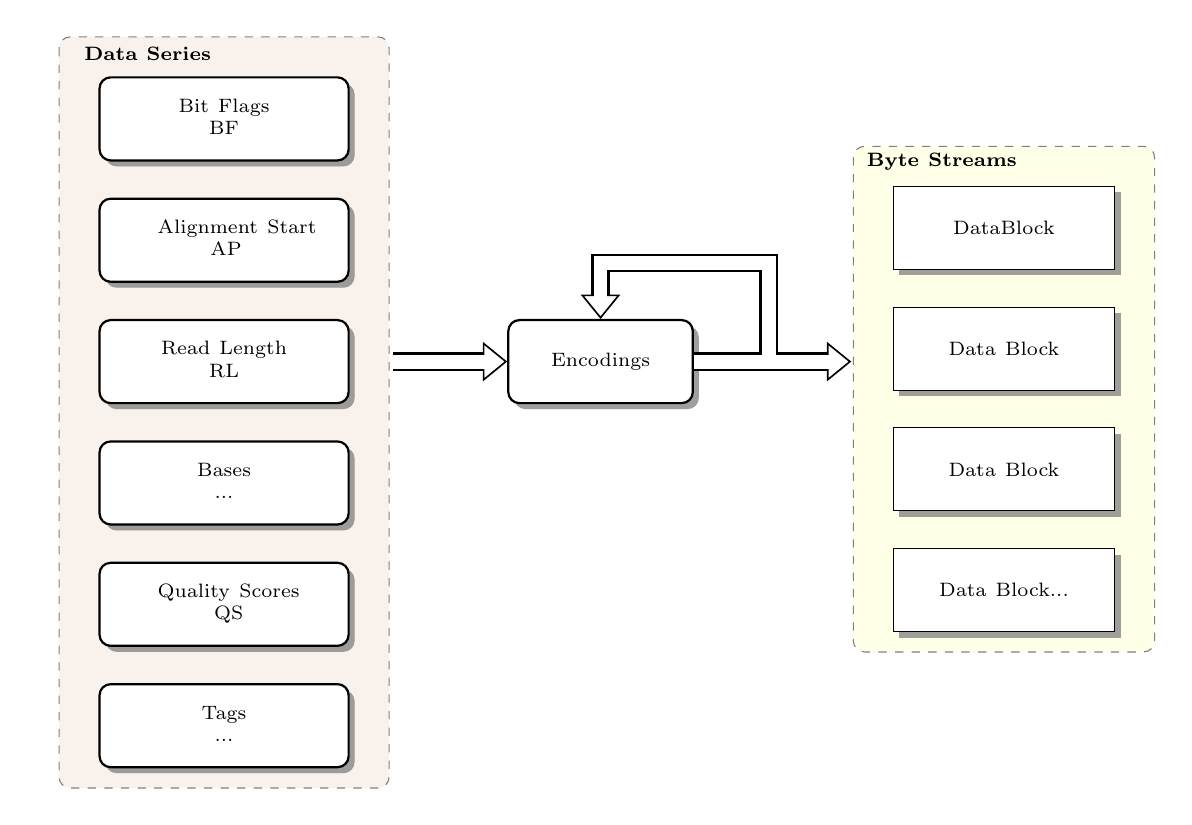
\begin{tikzpicture}[thick]

\usetikzlibrary{shapes, shadows, positioning, arrows,  decorations.markings, arrows.meta}

\pgfdeclarelayer{background}
\pgfsetlayers{background,main}

\tikzstyle{dsbox} = [blockbox, text width=6em, minimum width=9em, minimum height=3em, rounded corners, drop shadow]
\tikzstyle{blockbox}=[draw, fill=white, text width=4.0em, text centered, minimum height=1.0em, drop shadow]
\tikzstyle{encodedblock} = [blockbox, text width=6em, minimum width=8em, minimum height=3em, drop shadow]
\tikzstyle{encodings} = [dsbox, minimum width=6em, thick]

\tikzstyle{texto} = [above, text width=8em, text centered]

\tikzstyle{vecArrow} = [thick, decoration={markings,mark=at position
   1 with {\arrow[semithick]{Triangle[open, length=3.1mm, width=5mm]}}},
   double distance=5pt, shorten >= 8.5pt,
   preaction = {decorate},
   postaction = {draw,line width=5pt, white,shorten >= 8pt}]
\tikzstyle{innerWhite} = [semithick, white,line width=5pt, shorten >= 8pt]

\newcommand{\cramRecord}[6]{%
\begin{pgfonlayer}{background}
    \path (#1.west |- #1.north) + (-0.5, 0.5) node (a1) {};
    \path (#1.east |- #6.south) + (+0.5,-0.25) node (a2) {};
    \path[fill=brown!10,rounded corners, draw=black!50, dashed]
      (a1) rectangle (a2);
    \path (a1.east |- a1.south) + (1.0,-0.3) node[texto]
    {\scriptsize\textbf{Data Series}};
\end{pgfonlayer}}

\newcommand{\dsbox}[2]{node (p#1) [dsbox]
{\scriptsize{#2}}}
\newcommand{\encodedblock}[2]{node (p#1) [encodedblock]
	{\scriptsize{#2}}}
\newcommand{\encodedblocklarge}[2]{node (p#1) [encodedblocklarge]
   {\scriptsize{#2}}}

\path +(-2.5,-1.5) \dsbox{1}{\begin{tabular}{c} Bit Flags \\ BF \end{tabular}};
\path (p1.south)+(0.0,-1.0) \dsbox{2}{\begin{tabular}{c} Alignment Start\\ AP\quad\quad \end{tabular}};
\path (p2.south)+(0.0,-1.0) \dsbox{3}{\begin{tabular}{c} Read Length \\ RL \end{tabular}};
\path (p3.south)+(0.0,-1.0) \dsbox{4}{\begin{tabular}{c} Bases \\ ... \end{tabular}};
\path (p4.south)+(0.0,-1.0) \dsbox{5}{\begin{tabular}{c} Quality Scores \\ QS \end{tabular}};
\path (p5.south)+(0.0,-1.0) \dsbox{6}{\begin{tabular}{c} Tags \\ ... \end{tabular}};

\cramRecord{p1}{p2}{p3}{p4}{p5}{p6}

\newcommand{\blockStreams}[4]{%
\begin{pgfonlayer}{background}
    \path (#1.west |- #1.north)+(-0.5, 0.5) node (a3) {};
    \path (#4.east |- #4.south)+(+0.5, -0.25) node (a4) {};
    \path[fill=yellow!10, rounded corners, draw=black!50, dashed]
      (a3) rectangle (a4);
    \path (a3.east |- a3.south)+(1.0,-0.3) node[texto]{\scriptsize\textbf{Byte Streams}};
\end{pgfonlayer}}

\path (a1.south) + (12.0, -2.3) \encodedblock {7} {DataBlock};
\path (p7.south) + (0.0, -1.0)  \encodedblock {8} {Data Block};
\path (p8.south) + (0.0, -1.0)  \encodedblock {9} {Data Block}; 
\path (p9.south) + (0.0, -1.0)  \encodedblock {10}{Data Block...};

\blockStreams {p7} {p8} {p9} {p10}

\node (encodings) [encodings, right = 2 of p3] {\scriptsize Encodings};
\node (enc_e1) [right=0.7 of encodings] {};
\node (enc_e2) [right=1.05 of enc_e1] {};
\node (enc_n)  [above=1 of encodings.center] {};
\draw[vecArrow] (p3.east) + (0.55, 0) to (encodings.west);
\draw[vecArrow] (encodings.east) to (enc_e2.west);
\draw[vecArrow] (enc_e1.east) |- (enc_n.north) to (encodings.north);
\draw[innerWhite] (encodings.east) to (enc_e2.west);

\end{tikzpicture}

Figure 5: The relationship between Data Series, Possibly nested Encodings, and Data Blocks.

\end{center}

The picture shows how a CRAM record (on the left) is distributed to
multiple Data Blocks via a series of encodings.  Note the mapping from
Data Series to Blocks may be many to many, with the possibility of
multiple Data Series writing to the same Block and with a single
encoding such as BYTE\_ARRAY\_LEN potentially writing to two Blocks.


Each data series has an encoding. These encodings are stored in a map with byte[2] 
keys and are decoded in approximately this order\footnote{The precise order is defined in section~\ref{sec:record}.}:

\begin{threeparttable}[t]
\begin{tabular}{|l|l|>{\raggedright}p{100pt}|>{\raggedright}p{220pt}|}
\hline
\textbf{Key} & \textbf{Value data type} & \textbf{Name} & \textbf{Value}\tabularnewline
\hline
BF & encoding\texttt{<}int\texttt{>} & BAM bit flags & see separate section\tabularnewline
\hline
CF & encoding\texttt{<}int\texttt{>} & CRAM bit flags & see specific section\tabularnewline
\hline
RI & encoding\texttt{<}int\texttt{>} & reference id & record reference id from
the SAM file header\tabularnewline
\hline
RL & encoding\texttt{<}int\texttt{>} & read lengths & read lengths\tabularnewline
\hline
AP & encoding\texttt{<}int\texttt{>} & in-seq positions & if \textbf{AP-Delta} = true: 0-based alignment start
delta from the AP value in the previous record.
Note this delta may be negative, for example when switching references in a multi-reference slice.
When the record is the first in the slice, the previous position used is the slice alignment-start field (hence the first delta should be zero for single-reference slices, or the AP value itself for multi-reference slices).  \linebreak{}
if \textbf{AP-Delta} = false: encodes the alignment start position directly\tabularnewline
\hline
RG & encoding\texttt{<}int\texttt{>} & read groups & read groups. Special value 
`-1' stands for no group.\tabularnewline
\hline
RN\tnote{a} & encoding\texttt{<}byte[ ]\texttt{>} & read names & read names\tabularnewline
\hline
MF & encoding\texttt{<}int\texttt{>} & next mate bit flags & see specific section\tabularnewline
\hline
NS & encoding\texttt{<}int\texttt{>} & next fragment reference sequence id & reference 
sequence ids for the next fragment \tabularnewline
\hline
NP & encoding\texttt{<}int\texttt{>} & next mate alignment start & alignment positions 
for the next fragment\tabularnewline
\hline
TS & encoding\texttt{<}int\texttt{>} & template size & template sizes\tabularnewline
\hline
NF & encoding\texttt{<}int\texttt{>} & distance to next fragment & number of records
to the next fragment\tnote{b}\tabularnewline
\hline
TL\tnote{c} & encoding\texttt{<}int\texttt{>} & tag ids  & list of tag ids, see tag encoding
section\tabularnewline
\hline
FN & encoding\texttt{<}int\texttt{>} & number of read features & number of read
features in each record\tabularnewline
\hline
FC & encoding\texttt{<}byte\texttt{>} & read features codes & see separate section\tabularnewline
\hline
FP & encoding\texttt{<}int\texttt{>} & in-read positions & positions of the read
features; a positive delta to the last position (starting with zero)\tabularnewline
\hline
DL & encoding\texttt{<}int\texttt{>} & deletion lengths & base-pair deletion lengths\tabularnewline
\hline
BB & encoding\texttt{<}byte[ ]\texttt{>} & stretches of bases & bases\tabularnewline
\hline
QQ & encoding\texttt{<}byte[ ]\texttt{>} & stretches of quality scores & quality scores\tabularnewline
\hline
BS & encoding\texttt{<}byte\texttt{>} & base substitution codes & base substitution
codes\tabularnewline
\hline
IN & encoding\texttt{<}byte[ ]\texttt{>} & insertion & inserted bases\tabularnewline
\hline
RS & encoding\texttt{<}int\texttt{>} & reference skip length & number of skipped 
bases for the `N' read feature\tabularnewline
\hline
PD & encoding\texttt{<}int\texttt{>} & padding & number of padded bases\tabularnewline
\hline
HC & encoding\texttt{<}int\texttt{>} & hard clip & number of hard clipped bases\tabularnewline
\hline
SC & encoding\texttt{<}byte[ ]\texttt{>} & soft clip & soft clipped bases\tabularnewline
\hline
MQ & encoding\texttt{<}int\texttt{>} & mapping qualities & mapping quality scores\tabularnewline
\hline
BA & encoding\texttt{<}byte\texttt{>} & bases & bases\tabularnewline
\hline
QS & encoding\texttt{<}byte\texttt{>} & quality scores & quality scores\tabularnewline
\hline
\end{tabular}

\begin{tablenotes}
\item[a] Note RN this is decoded after MF if the record is detached from the mate and we are attempting to auto-generate read names.
\item[b] The count is reset for each slice so NF can only refer to a record later within this slice.
\item[c] Decode of TL is followed by decoding the tag values themselves, in order of appearance in the tag dictionary.
\end{tablenotes}
\end{threeparttable}

\subsubsection{Tag encoding map}
\label{subsubsec:tags}

The tag dictionary (TD) describes the unique combinations of tag id / type that occur on each alignment record.
For example if we search the id / types present in each record and find only two combinations -- X1:i BC:Z SA:Z: and X1:i: BC:Z -- then we have two dictionary entries in the TD map.

Let $L_{i}=\{T_{i0}, T_{i1}, \ldots, T_{ix}\}$ be a list of all tag ids for a record $R_{i}$, where $i$ is the sequential record index and $T_{ij}$ denotes $j$-th tag id in the record.
The list of unique $L_{i}$ is stored as the TD value in the preservation map.
Maintaining the order is not a requirement for encoders (hence ``combinations''), but it is permissible and thus different permutations, each encoded with their own elements in TD, should be supported by the decoder.
Each $L_{i}$ element in TD is assigned a sequential integer number starting with 0.
These integer numbers are referred to by the TL data series.
Using TD, an integer from the TL data series can be mapped back into a list of tag ids.
Thus per alignment record we only need to store tag values and not their ids and types.

The TD is written as a byte array consisting of $L_{i}$ values separated with \textbackslash{}0.
Each $L_{i}$ value is written as a concatenation of 3 byte $T_{ij}$ elements: tag id followed by BAM tag type code (one of A, c, C, s, S, i, I, f, F, Z, H or B, as described in the SAM specification) or \texttt{*}.
Type code \texttt{*} is used as a placeholder to mark the presence and location of the MD, NM or RG tags.

For example the TD for tag lists X1:i BC:Z SA:Z and X1:i MD:Z NM:i BC:Z may be encoded as\\
X1CBCZSAZ\textbackslash{}0X1CMD*NM*BCZ\textbackslash{}0, with X1C indicating a 1 byte unsigned value for tag X1 and an assumption that all MD and NM tags present can be auto-generated.

\subsubsection*{Tag values}

The encodings used for different tags are stored in a map.
The key is 3 bytes formed from the BAM tag id and type code, matching the TD dictionary described above.
Unlike the Data Series Encoding Map, the key is stored in the map as a uint7 encoded integer, constructed using $(char1<<16) + (char2<<8) + type$.
For example, the 3-byte representation of OQ:Z is \{0x4F, 0x51, 0x5A\} and these bytes are intepreted as the integer key 0x004F515A, leading to an uint7 byte stream \{0x82, 0xbd, 0xa2, 0x59\}.

\begin{tabular}{|l|l|l|>{\raggedright}p{160pt}|}
\hline
\textbf{Key} & \textbf{Value data type} & \textbf{Name} & \textbf{Value}
\tabularnewline
\hline
TAG ID 1:TAG TYPE 1 & encoding\texttt{<}byte[ ]\texttt{>} & read tag 1 & tag values
(names and types are available in the data series code)\tabularnewline
\hline
... &  & ... & ...\tabularnewline
\hline
TAG ID N:TAG TYPE N & encoding\texttt{<}byte[ ]\texttt{>} & read tag N & ...\tabularnewline
\hline
\end{tabular}

Note that tag values are encoded as array of bytes. The routines to convert tag 
values into byte array and back are the same as in BAM with the exception of value 
type being captured in the tag key rather in the value.
Hence consuming 1 byte for types `C' and `c', 2 bytes for types `S' and `s', 4 bytes for types `I', `i' and `f', and a variable number of bytes for types `H', `Z' and `B'.

\subsection{Slice header block}

The slice header block is never compressed (block method=raw). For reference mapped 
reads the slice header also defines the reference sequence context of the data 
blocks associated with the slice. Mapped reads can be stored along with
\textbf{placed unmapped}\footnote{Unmapped reads can be \textit{placed} or \textit{unplaced}.
A read that is unmapped according to bit 0x4 of the BF (BAM bit flags)
data series, but has position and reference fields filled in, is
\textit{placed unmapped}.  In contrast, \textit{unplaced unmapped}
reads have have a reference sequence ID of -1 and alignment position of 0.}
reads on the same reference within the same slice.

Slices with the Multiple Reference flag (-2) set as the sequence ID in the header may contain reads
mapped to multiple external references, including unmapped\footnotemark[\value{footnote}] reads (placed on these references or unplaced),
but multiple embedded references cannot be combined in this way.  When multiple references are
used, the RI data series will be used to determine the reference sequence ID for each record.  This
data series is not present when only a single reference is used within a slice.

The Unmapped (-1) sequence ID in the header is for slices containing only unplaced
unmapped\footnotemark[\value{footnote}] reads.

A slice containing data that does not use the external reference in
any sequence may set the reference MD5 sum to zero.  This can happen
because the data is unmapped or the sequence has been stored verbatim
instead of via reference-differencing.  This latter scenario is
recommended for unsorted or non-coordinate-sorted data.

The slice header block contains the following fields.

\begin{tabular}{|l|l|>{\raggedright}p{200pt}|}
\hline
\textbf{Data type} & \textbf{Name} & \textbf{Value}\tabularnewline
\hline
int7 & reference sequence id & reference sequence identifier or\linebreak{}
-1 for unmapped reads\linebreak{}
-2 for multiple reference sequences.\linebreak{}
This value must match that of its enclosing container.\tabularnewline
\hline
uint7 & alignment start & the alignment start position.\linebreak{}
0 if the slice is multiple-reference
or contains unmapped unplaced reads\tabularnewline
\hline
uint7 & alignment span & the length of the alignment.\linebreak{}
0 if the slice is multiple-reference
or contains unmapped unplaced reads\tabularnewline
\hline
uint7 & number of records & the number of records in the slice\tabularnewline
\hline
uint7 & record counter & 1-based sequential index of records in the file/stream\tabularnewline
\hline
uint7 & number of blocks & the number of blocks in the slice\tabularnewline
\hline
uint7[ ] & block content ids & block content ids of the blocks in the slice\tabularnewline
\hline
uint7 & embedded reference bases block content id & block content id for the embedded 
reference sequence bases or 0 for none\tabularnewline
\hline
byte[16] & reference md5 & MD5 checksum of the reference bases within the slice 
boundaries.  If this slice has reference sequence id of -1 (unmapped) or -2 (multi-ref)
the MD5 should be 16 bytes of \textbackslash{}0. For embedded references, the MD5
can either be all-zeros or the MD5 of the embedded sequence.\tabularnewline
\hline
byte[] & optional tags & a series of tag,type,value tuples encoded as
per BAM auxiliary fields.\tabularnewline
\hline
\end{tabular}

The optional tags are encoded in the same manner as BAM tags.  I.e. a
series of binary encoded tags concatenated together where each tag
consists of a 2 byte key (matching [A-Za-z][A-Za-z0-9]) followed by a
1 byte type ([AfZHcCsSiIB]) followed by a string of bytes in a format
defined by the type.

Tags starting in a capital letter are reserved while lowercase ones or
those starting with X, Y or Z are user definable.  Any tag not
understood by a decoder should be skipped over without producing an
error.

At present no tags are defined, but potential uses include additional
checksums and statistical information.

% Details omitted until we fully work through all the corner cases,
% such as seq/qual of *.
%
% Reserved tags are defined as follows:
% 
% \begin{tabular}{|l|l|>{\raggedright}p{325pt}|}
% \hline
% \textbf{Tag type} & \textbf{BAM format} & \textbf{Meaning}\tabularnewline
% \hline
% BD & i & Sum over all reads of the CRC32 hash of sequence base.  This
% may be used to validate round-trips in and out of CRAM.
% calls\tabularnewline
% \hline
% SD & i & Sum over all reads of the CRC32 hash of quality scores. (If
% the quality string is ``*'' in SAM then the hash is of the BAM encoded
% version - a string of bytes with value 255.)\tabularnewline
% \hline
% \end{tabular}


\subsection{End of file container}

A special container is used to mark the end of a file or stream. It is required in version 3 or later.
The idea is to provide an easy and a quick way to detect that a CRAM file or stream is complete.
The marker is an empty container with ref seq id set to -1 (unaligned) and alignment start set to 4542278 (which is ``EOF'' when seen in ASCII).

It is recommended that implementations of CRAM validate EOF by checking these values rather than direct comparison of byte values, as these checks will be valid for all versions of CRAM

\section{Record structure}
\label{sec:record}

CRAM record is based on the SAM record but has additional features allowing for 
more efficient data storage.  In contrast to BAM record CRAM records
are separated by type of data into a series of data blocks.  These
blocks can then use content type aware compression techniques.

As CRAM data series may be interleaved within the same blocks\footnote{Interleaving can sometimes provide better compression, however it also adds dependency between types of data meaning it is not possible to selectively decode one data series if it co-locates with another data series in the same block.} understanding the order in which CRAM data series must be decoded is vital.

The overall flowchart is below, with more detailed description in the subsequent sections.

\algnewcommand\algorithmicto{\text{ \textbf{to} }}

\subsection{CRAM record}

Both mapped and unmapped reads start with the following fields. Please note that 
the data series type refers to the logical data type and the data series name corresponds 
to the data series encoding map.

\begin{tabular}{|>{\raggedright}p{70pt}|>{\raggedright}p{75pt}|>{\raggedright}p{90pt}|>{\raggedright}p{171pt}|}
\hline
\textbf{Data series type} & \textbf{Data series name} & \textbf{Field} & \textbf{Description}\tabularnewline
\hline
uint & BF & BAM bit flags & see BAM bit flags below\tabularnewline
\hline
uint & CF & CRAM bit flags & see CRAM bit flags below\tabularnewline
\hline
- & - & Positional data & See section \ref{subsec:positions}\tabularnewline
\hline
- & - & Read names & See section \ref{subsec:names}\tabularnewline
\hline
- & - & Mate records & See section \ref{subsec:mate}\tabularnewline
\hline
- & - & Auxiliary tags & See section \ref{subsec:tags}\tabularnewline
\hline
- & - & Sequences & See sections \ref{subsec:mapped} and \ref{subsec:unmapped}\tabularnewline
\hline
\end{tabular}

\subsubsection*{BAM bit flags (BF data series)}

The following flags are duplicated from the SAM and BAM specification, with identical meaning.
Note however some of these flags can be derived during decode, so may be omitted in the CRAM file and the bits computed based on both reads of a pair-end library residing within the same slice.

\begin{threeparttable}[t]
\begin{tabular}{|l|l|l|}
\hline
\textbf{Bit flag} & \textbf{Comment} & \textbf{Description}\tabularnewline
\hline
0x1 &  & template having multiple segments in sequencing\tabularnewline
\hline
0x2 &  & each segment properly aligned according to the aligner\tabularnewline
\hline
0x4 &  & segment unmapped\tnote{a}\tabularnewline
\hline
0x8 & calculated\tnote{b}\ \ or stored in the mate's info & next segment in template unmapped\tabularnewline
\hline
0x10 &  & SEQ being reverse complemented\tabularnewline
\hline
0x20 & calculated\tnote{b}\ \ or stored in the mate's info & SEQ of the next segment in the
template being reverse complemented\tabularnewline
\hline
0x40 &  & the first segment in the template\tnote{c}\tabularnewline
\hline
0x80 &  & the last segment in the template\tnote{c}\tabularnewline
\hline
0x100 &  & secondary alignment\tabularnewline
\hline
0x200 &  & not passing quality controls\tabularnewline
\hline
0x400 &  & PCT or optical duplicate\tabularnewline
\hline
0x800 &  & Supplementary alignment\tabularnewline
\hline
\end{tabular}
\begin{tablenotes}
\item[a] Bit 0x4 is the only reliable place to tell whether the read is unmapped.  If 0x4 is set, no assumptions may be made about bits 0x2, 0x100 and 0x800.
\item[b] For segments within the same slice.
\item[c] Bits 0x40 and 0x80 reflect the read ordering within each template inherent in the sequencing technology used, which may be independent from the actual mapping orientation.
If 0x40 and 0x80 are both set, the read is part of a linear template (one where the template sequence is expected to be in a linear order), but it is neither the first nor the last read.
If both 0x40 and 0x80 are unset, the index of the read in the template is unknown.
This may happen for a non-linear template (such as one constructed by stitching together other templates) or when this information is lost during data processing.
\end{tablenotes}
\end{threeparttable}

\subsubsection*{CRAM bit flags (CF data series)}

The CRAM bit flags (also known as compression bit flags) expressed as an integer represent the CF data series. 
The following compression flags are defined for each CRAM read record:

\begin{tabular}{|>{\raggedright}p{39pt}|>{\raggedright}p{150pt}|>{\raggedright}p{242pt}|}
\hline
\textbf{Bit flag} & \textbf{Name} & \textbf{Description}\tabularnewline
\hline
0x1 & quality scores stored as array & quality scores can be stored as read features
or as an array similar to read bases.\tabularnewline
\hline
0x2 & detached & mate information is stored verbatim (e.g. because the pair spans multiple slices or the fields differ to the CRAM computed method)\tabularnewline
\hline
0x4 & has mate downstream & tells if the next segment should be expected further
in the stream\tabularnewline
\hline
0x8 & decode sequence as ``*'' & informs the decoder that the sequence
is unknown and that any encoded reference differences are present only to
recreate the CIGAR string.\tabularnewline
\hline
0x10 & explicit template size & decode from the template size (TS) data series even for record in an attached pair.\tabularnewline
\hline
\end{tabular}


The following pseudocode describes the general process of decoding an entire CRAM record.
The sequence data itself is in one of two encoding formats depending on whether the record is aligned (mapped).

\subsubsection*{Decode pseudocode}
\newlength{\maxwidth}
\newcommand{\algalign}[2] % #1 = text to left, #2 = text to right
{\makebox[\maxwidth][l]{$#1{}$}${}#2$}

\begin{algorithmic}[1]
\Procedure{DecodeRecord}{}
\settowidth{\maxwidth}{CRAM\_flags\quad}
\State \algalign{BAM\_flags}{\gets}  \Call{ReadItem}{BF, Integer}
\State \algalign{CRAM\_flags}{\gets} \Call{ReadItem}{CF, Integer}
\State \Call{DecodePositions}{}\Comment{See section \ref{subsec:positions}}
\State \Call{DecodeNames}{}\Comment{See section \ref{subsec:names}}
\State \Call{DecodeMateData}{}\Comment{See section \ref{subsec:mate}}
\State \Call{DecodeTagData}{}\Comment{See section \ref{subsec:tags}}
\Statex

\If{$(BF$ AND $4) \ne 0$}\Comment{Unmapped flag}
  \State \Call{DecodeMappedRead}{}\Comment{See section \ref{subsec:mapped}}
\Else
  \State \Call{DecodeUnmappedRead}{}\Comment{See section \ref{subsec:unmapped}}
\EndIf
\EndProcedure
\end{algorithmic}

\subsection{CRAM positional data}
\label{subsec:positions}

Following the bit-wise BAM and CRAM flags, CRAM encodes positional related data including reference, alignment positions and length, and read-group.
Positional data is stored for both mapped and unmapped sequences, as unmapped data may still be ``placed'' at a specific location in the genome (without being aligned).
Typically this is done to keep a sequence pair (paired-end or mate-pair sequencing libraries) together when one of the pair aligns and the other does not.

For reads stored in a position-sorted slice, the AP-delta flag in the compression header preservation map should be set and the AP data series will be delta encoded, using the slice alignment-start value as the first position to delta against.
Note for multi-reference slices this may mean that the AP series includes negative values, such as when moving from an alignment to the end of one reference sequence to the start of the next or to unmapped unplaced data.  When the AP-delta flag is not set the AP data series is stored as a normal integer value.

\begin{tabular}{|>{\raggedright}p{70pt}|>{\raggedright}p{75pt}|>{\raggedright}p{90pt}|>{\raggedright}p{171pt}|}
\hline
\textbf{Data series type} & \textbf{Data series name} & \textbf{Field} & \textbf{Description}\tabularnewline
\hline
int & RI & ref id & reference sequence id (only present in multiref slices)\tabularnewline
\hline
int & RL & read length & the length of the read\tabularnewline
\hline
int & AP & alignment start & the alignment start position\tabularnewline
\hline
int & RG & read group & the read group identifier expressed as the N\textsuperscript{th} record in the header, starting from 0 with -1 for no group\tabularnewline
\hline
\end{tabular}

\vskip 20pt
\begin{algorithmic}[1]
\Procedure{DecodePositions}{}
\If{$slice\_header.reference\_sequence\_id = -2$}
  \State $reference\_id\gets$ \Call{ReadItem}{RI, Integer}
\Else
  \State $reference\_id\gets slice\_header.reference\_sequence\_id$
\EndIf
\State $read\_length \gets$ \Call{ReadItem}{RL, Integer}
\If{$container\_pmap.AP\_delta \ne 0$}
    \If{$first\_record\_in\_slice$}
        \State $last\_position\gets$ $slice\_header.alignment\_start$
    \EndIf
    \State $alignment\_position \gets$ \Call{ReadItem}{AP, Integer} + $last\_position$
    \State $last\_position \gets alignment\_position$
\Else
    \State $alignment\_position \gets$ \Call{ReadItem}{AP, Integer}
\EndIf
\State $read\_group \gets$ \Call{ReadItem}{RG, Integer}
\EndProcedure
\end{algorithmic}

\subsection{Read names (RN data series)}
\label{subsec:names}

Read names can be preserved in the CRAM format, but this is optional and is governed by the \texttt{RN} preservation map key in the container compression header. See section \ref{subsec:compression-header}.
When read names are not preserved the CRAM decoder should generate names, typically based on the file name and a numeric ID of the read using the record counter field of the slice header block.
Note read names may still be preserved even when the \texttt{RN} compression header key indicates otherwise, such as where a read is part of a read-pair and the pair spans multiple slices.
In this situation the record will be marked as detached (see the CF data series) and the mate data below (section \ref{subsec:mate}) will contain the read name.

\begin{tabular}{|>{\raggedright}p{70pt}|>{\raggedright}p{75pt}|>{\raggedright}p{90pt}|>{\raggedright}p{171pt}|}
\hline
\textbf{Data series type} & \textbf{Data series name} & \textbf{Field} & \textbf{Description}\tabularnewline
\hline
byte[] & RN & read names & read names\tabularnewline
\hline
\end{tabular}

\vskip 20pt
\begin{algorithmic}[1]
\Procedure{DecodeNames}{}
\State $read\_name \gets empty$
\If{$container\_pmap.read\_names\_included = 1$}
  \State $read\_name \gets$ \Call{ReadItem}{RN, Byte[]}
\EndIf
\Statex
\EndProcedure
\end{algorithmic}

\subsection{Mate record}
\label{subsec:mate}

There are two ways in which mate information can be preserved in CRAM: number of records downstream (distance, within this slice) to the next fragment in the template and a special mate record if the next fragment is not in the current slice.
In the latter case the record is labelled as ``detached'', see the CF data series.

For mates within the slice only the distance is captured, and only for the first record.  The mate has neither detached nor downstream flags set in the CF data series.

\begin{tabular}{|>{\raggedright}p{68pt}|>{\raggedright}p{115pt}|>{\raggedright}p{228pt}|}
\hline
\textbf{Data series type} & \textbf{Data series name} & \textbf{Description}\tabularnewline
\hline
int & NF & the number of records to the next fragment\tabularnewline
\hline
\end{tabular}

In the above case, the NS (mate reference name), NP (mate position) and TS (template size) fields for both records should be derived once the mate has also been decoded.
Mate reference name and position are obvious and simply copied from the mate.
The template size is computed using the method described in the SAM specification; the inclusive distance from the leftmost to rightmost mapped bases with the sign being positive for the leftmost record and negative for the rightmost record.

If the next fragment is not found within this slice then the following structure is included into the CRAM record.
Note there are cases where read-pairs within the same slice may be marked as detached and use this structure, such as to store mate-pair information that does not match the algorithm used by CRAM for computing the mate data on-the-fly.

\begin{tabular}{|>{\raggedright}p{66pt}|>{\raggedright}p{117pt}|>{\raggedright}p{228pt}|}
\hline
\textbf{Data series type} & \textbf{Data series name} & \textbf{Description}\tabularnewline
\hline
int & MF & next mate bit flags, see table below\tabularnewline
\hline
byte[ ] & RN & the read name (if and only if not known already)\tabularnewline
\hline
int & NS & mate reference sequence identifier \tabularnewline
\hline
int & NP & mate alignment start position \tabularnewline
\hline
int & TS & the size of the template (insert size)\tabularnewline
\hline
\end{tabular}

\subsubsection*{Next mate bit flags (MF data series)}

The next mate bit flags expressed as an integer represent the MF data series.
These represent the missing bits we excluded from the BF data series (when compared to the full SAM/BAM flags).
The following bit flags are defined:

\begin{tabular}{|>{\raggedright}p{47pt}|>{\raggedright}p{134pt}|>{\raggedright}p{250pt}|}
\hline
\textbf{Bit flag} & \textbf{Name} & \textbf{Description}\tabularnewline
\hline
0x1 & mate negative strand bit & the bit is set if the mate is on the negative
strand\tabularnewline
\hline
0x2 & mate unmapped bit & the bit is set if the mate is unmapped\tabularnewline
\hline
\end{tabular}


\subsubsection*{Decode mate pseudocode}

\begin{algorithmic}[1]
\Procedure{DecodeMateData}{}
\If{$CF\bitand 2$}\Comment{Detached from mate}
  \State $mate\_flags\gets $ \Call{ReadItem}{MF,Integer}
  \If{$mate\_flags\bitand 1$}
    \State $bam\_flags\gets bam\_flags\bitor$ 0x20\Comment{Mate is reverse-complemented}
  \EndIf
  \If{$mate\_flags\bitand 2$}
    \State $bam\_flags\gets bam\_flags\bitor$ 0x08\Comment{Mate is unmapped}
  \EndIf
  \If{$container\_pmap.read\_names\_included \ne 1$}
    \State $read\_name \gets$ \Call{ReadItem}{RN, Byte[]}
  \EndIf
\settowidth{\maxwidth}{mate\_position\ }
\State \algalign{mate\_ref\_id}{\gets}  \Call{ReadItem}{NS, Integer}
\State \algalign{mate\_position}{\gets} \Call{ReadItem}{NP, Integer}
\State \algalign{template\_size}{\gets} \Call{ReadItem}{TS, Integer}
\ElsIf{$CF\bitand 16$}\Comment{Explicit template size}
  \State $template\_size\gets$ \Call{ReadItem}{TS, Integer}
\EndIf
\EndProcedure
\end{algorithmic}

Note as with the SAM specification a template may be permitted to have more than two alignment records.
In this case the ``mate'' for each record is considered to be the next record, with the mate for the last record being the first to form a circular list.
The above algorithm is a simplification that does not deal with this scenario.
The full method needs to observe when record $this+NF$ is also labelled as having an additional mate downstream.
One recommended approach is to resolve the mate information in a second pass, once the entire slice has been decoded.
The final segment in the mate chain needs to set $bam\_flags$ fields 0x20 and 0x08 accordingly based on the first segment.
This is also not listed in the above algorithm, for brevity.

\subsection{Auxiliary tags}
\label{subsec:tags}

Tags are encoded using a tag line (TL data series) integer into the tag dictionary (TD field in the compression header preservation map, see section \ref{subsec:compression-header}).
See section \ref{subsubsec:tags} for a more detailed description of this process.

\begin{tabular}{|>{\raggedright}p{70pt}|>{\raggedright}p{75pt}|>{\raggedright}p{90pt}|>{\raggedright}p{200pt}|}
\hline
\textbf{Data series type} & \textbf{Data series name} & \textbf{Field} & \textbf{Description}\tabularnewline
\hline
int & TL & tag line & an index into the tag dictionary (TD)\tabularnewline
\hline
\textit{various} & \textit{various} & tag name/type & 3 character key (2 tag identifier and 1 tag type), as specified by the tag dictionary\tabularnewline
\hline
\end{tabular}

\vskip 20pt
\begin{algorithmic}[1]
\Procedure{DecodeTagData}{}
\State $tag\_line\gets$ \Call{ReadItem}{TL,Integer}
\ForAll {$ele \in container\_pmap.tag\_dict(tag\_line)$}
  \State $name\gets$ first two characters of $ele$
  \State $tag(type)\gets$ last character of $ele$
  \If{$tag(type) = ``*''$}
  \State $tag(name)\gets$ \Call{GenerateTag}{$name$}
  \Else
  \State $tag(name)\gets$ \Call{ReadItem}{$ele$, Byte[]}\Comment{Type specific}
  \EndIf
\EndFor
\EndProcedure
\end{algorithmic}

In the above procedure, $name$ is a two letter tag name and $type$ is one of the permitted types documented in the SAM/BAM specification.
Type is \texttt{c} (signed 8-bit integer), \texttt{C} (unsigned 8-bit integer), \texttt{s} (signed 16-bit integer), \texttt{S} (unsigned 16-bit integer), \texttt{i} (signed 32-bit integer), \texttt{I} (unsigned 32-bit integer), \texttt{f} (32-bit float), \texttt{Z} (nul-terminated string), \texttt{H} (nul-terminated string of hex digits) and \texttt{B} (binary data in array format with the first byte being one of c,C,s,S,i,I,f using the meaning above, a 32-bit integer for the number of array elements, followed by array data encoded using the specified format).  All integers are little endian encoded.

For example a SAM tag \texttt{MQ:i} has name \texttt{MQ} and type \texttt{i} and will be decoded using one of MQc, MQC, MQs, MQS, MQi and MQI data series depending on size and sign of the integer value.

Note some auxiliary tags can be created automatically during decode so can optionally be removed by the encoder.
However if the decoder finds a tag stored verbatim it should use this in preference to automatically computing the value.

The RG (read group) auxiliary tag should be created if the read group (RG data series) value is not $-1$.

The MD and NM auxiliary tags store the differences (an edit string) between the sequence and the reference along with the number of mismatches.
These may optionally be created on-the-fly during reference-based sequence reconstruction and should match the description provided in the SAMtags document.
An encoder may decide to store these verbatim when no reference is used or where the automatically constructed values differ to the input data.

The tag type \texttt{*} is used in conjunction with MD, NM and RG as a flag to indicate that this tag is present but is not being stored verbatim.
(If MD is being stored verbatim, we would expect MDZ in the TD dictionary for this tag line.)
The \texttt{*} type is also useful for ensuring the ordering of tags can be preserved.

Note it is permitted for decoders to choose to auto-generate MD and NM tags even in the absence of MD* and NM* entries.

\subsection{Mapped reads}
\label{subsec:mapped}

\subsubsection*{Read feature records}
\label{subsec:features}

Read features are used to store read details that are expressed using read coordinates 
(e.g. base differences respective to the reference sequence). The read feature 
records start with the number of read features followed by the read features themselves.
Each read feature has the position encoded as the distance since the
last feature position, or the absolute position (i.e. delta vs zero)
for the first feature.
Finally the single mapping quality and per-base quality scores are stored.

\begin{threeparttable}[t]
\begin{tabular}{|>{\raggedright}p{88pt}|>{\raggedright}p{83pt}|>{\raggedright}p{85pt}|>{\raggedright}p{180pt}|}
\hline
\textbf{Data series type} & \textbf{Data series name} & \textbf{Field} & \textbf{Description}\tabularnewline
\hline
int & FN & number of read features & the number of read features\tabularnewline
\hline
int & FP & in-read-position\tnote{a} & position of the read feature\tabularnewline 
\hline
byte & FC & read feature code\tnote{a} & See feature codes below\tabularnewline
\hline
* & * & read feature data\tnote{a} & See feature codes below\tabularnewline
\hline
int & MQ & mapping qualities & mapping quality score\tabularnewline
\hline
byte[read length] & QS & quality scores & the base qualities, if preserved\tabularnewline
\hline
\end{tabular}
\begin{tablenotes}
\item[a] Repeated FN times, once for each read feature.
\end{tablenotes}
\end{threeparttable}

\subsubsection*{Read feature codes}

Each feature code has its own associated data series containing further information specific to that feature.
The following codes are used to distinguish variations in read coordinates:

\begin{tabular}{|>{\raggedright}p{91pt}|>{\raggedright}p{45pt}|>{\raggedright}p{72pt}|>{\raggedright}p{66pt}|>{\raggedright}p{132pt}|}
\hline
\textbf{Feature code} & \textbf{Id} & \textbf{Data series type} & \textbf{Data 
series name} & \textbf{Description}\tabularnewline
\hline
Bases & b (0x62) & byte[ ] & BB & a stretch of bases\tabularnewline
\hline
Scores & q (0x71) & byte[ ] & QQ & a stretch of scores\tabularnewline
\hline
% Neither C nor Java implementations generator nor can decode the 'A'
% feature code, but if they did they'd be BB/QQ and not BA/QS.  Best
% to omit it from published spec for now?
%
% Bases and scores & A (0x41) & byte[ ],byte[ ] & BB,QQ & A a stretch of bases and
% quality scores score\tabularnewline
% \hline
Read base & B (0x42) & byte,byte & BA,QS & A base and associated quality score\tabularnewline
\hline
Substitution & X (0x58) & byte & BS & base substitution codes, SAM operators X, 
M and =\tabularnewline
\hline
Insertion & I (0x49) & byte[ ] & IN & inserted bases, SAM operator I\tabularnewline
\hline
Deletion & D (0x44) & int & DL & number of deleted bases, SAM operator D\tabularnewline
\hline
Insert base & i (0x69) & byte & BA & single inserted base, SAM operator I\tabularnewline
\hline
Quality score & Q (0x51) & byte & QS & single quality score\tabularnewline
\hline
Reference skip & N (0x4E) & int & RS & number of skipped bases, SAM operator N\tabularnewline
\hline
Soft clip & S (0x53) & byte[ ] & SC & soft clipped bases, SAM operator S\tabularnewline
\hline
Padding & P (0x50) & int & PD & number of padded bases, SAM operator P\tabularnewline
\hline
Hard clip & H (0x48) & int & HC & number of hard clipped bases, SAM operator H\tabularnewline
\hline
\end{tabular}

\subsubsection*{Base substitution codes (BS data series)}

A base substitution is defined as a change from one nucleotide base (reference base) to
another (read base), including N as an unknown or missing base. There are 5 possible reference
bases (ACGTN), with 4 possible substitutions for each base, and 20 substitutions in total.
The codes for all possible substitutions are stored in a substitution matrix. To restore a
base, one would use the reference base and the substitution code, resolving the base via lookup
in the substitution matrix.

\subsubsection*{Substitution Matrix Format}

Each of the 4 possible substitutions for a given reference base is assigned a 2-bit integer
code (see below) with a value ranging from 0 to 3 inclusive. The 4 2-bit codes are packed
into a single byte, high 2-bits first, for each base ACGTN (minus the reference base itself).
The entire substitution matrix is written as 5 such bytes, one for each reference base, also
in the order ACGTN.

\subsubsection*{Substitution Code Assignment}

To assign the susbtitution code for a given reference base/read base, the substitutions for
each reference base may optionally be sorted by their frequencies, in descending order, with
same-frequency ties broken using the fixed order ACGTN. Although sorting by substitution
frequency is not required by the CRAM format, assigning substitution codes based on frequency
maximizes compression by ensuring that the most frequent substitutions use the shortest possible
codes.

For example, let us assume the following substitution frequencies for base A: 

AC: 15\%

AG: 25\%

AT: 55\%

AN: 5\%

Then the substitution codes are: 

AC: 2

AG: 1

AT: 0

AN: 3

The first byte of the substitution matrix entry for reference base A is written as a single byte,
with the codes in the order CGTN: 10 01 00 11 = 147 decimal, or 0x93 in this case. This will then
be followed by 4 more bytes representing substitutions for reference bases C, G, T and N.

\subsubsection*{Decode mapped read pseudocode}

\begin{algorithmic}[1]
\Procedure{DecodeMappedRead}{}
  \State $feature\_number\gets$ \Call{ReadItem}{FN, Integer} 
  \State $last\_feature\_position\gets 0$
  \For{$i\gets 1 \algorithmicto feature\_number$}
    \State \Call{DecodeFeature}{}
  \EndFor
  \State $mapping\_quality\gets$ \Call{ReadItem}{MQ, Integer} 
  \If{$container\_pmap.preserve\_quality\_scores$}
    \If{$(container\_pmap.qual\_orientation = 0) \logand (bam\_flags \bitand 0x10)$}
      \For{$i\gets 0 \algorithmicto read\_length-1$}
        \State $quality\_score_{read\_length-1-i}\gets$ \Call{ReadItem}{QS, Integer} 
       \EndFor
    \Else
      \For{$i\gets 0 \algorithmicto read\_length-1$}
        \State $quality\_score_i\gets$ \Call{ReadItem}{QS, Integer} 
       \EndFor
    \EndIf
  \EndIf
\EndProcedure
\Statex
\Procedure{DecodeFeature}{}
    \settowidth{\maxwidth}{feature\_position\ }
    \State \algalign{feature\_code}{\gets}       \Call{ReadItem}{FC, Integer} 
    \State \algalign{feature\_position}{\gets}   \Call{ReadItem}{FP, Integer} $+\ last\_feature\_position$
    \State $last\_feature\_position\gets feature\_position$
    \settowidth{\maxwidth}{substitution\_code\ }
    \If{$feature\_code = $`B'}
      \State \algalign{base}{\gets}              \Call{ReadItem}{BA, Byte}
      \State \algalign{quality\_score}{\gets}    \Call{ReadItem}{QS, Byte}
    \ElsIf{$feature\_code = $`X'}
      \State \algalign{substitution\_code}{\gets} \Call{ReadItem}{BS, Byte}
    \ElsIf{$feature\_code = $`I'}
      \State \algalign{inserted\_bases}{\gets}   \Call{ReadItem}{IN, Byte[]}
    \ElsIf{$feature\_code = $`S'}
      \State \algalign{softclip\_bases}{\gets}   \Call{ReadItem}{SC, Byte[]}
    \ElsIf{$feature\_code = $`H'}
      \State \algalign{hardclip\_length}{\gets}  \Call{ReadItem}{HC, Integer}
    \ElsIf{$feature\_code = $`P'}
      \State \algalign{pad\_length}{\gets}       \Call{ReadItem}{PD, Integer}
    \ElsIf{$feature\_code = $`D'}
      \State \algalign{deletion\_length}{\gets}  \Call{ReadItem}{DL, Integer}
    \ElsIf{$feature\_code = $`N'}
      \State \algalign{ref\_skip\_length}{\gets} \Call{ReadItem}{RS, Integer}
    \ElsIf{$feature\_code = $`i'}
      \State \algalign{base}{\gets}              \Call{ReadItem}{BA, Byte}
    \ElsIf{$feature\_code = $`b'}
      \State \algalign{bases}{\gets}             \Call{ReadItem}{BB, Byte[]}
    \ElsIf{$feature\_code = $`q'}
      \State \algalign{quality\_scores}{\gets}   \Call{ReadItem}{QQ, Byte[]}
    \ElsIf{$feature\_code = $`Q'}
      \State \algalign{quality\_score}{\gets}    \Call{ReadItem}{QS, Byte}
    \EndIf
\EndProcedure
\end{algorithmic}

\subsection{Unmapped reads}
\label{subsec:unmapped}

The CRAM record structure for unmapped reads has the following additional fields:

\begin{tabular}{|>{\raggedright}p{88pt}|>{\raggedright}p{83pt}|>{\raggedright}p{85pt}|>{\raggedright}p{180pt}|}
\hline
\textbf{Data series type} & \textbf{Data series name} & \textbf{Field} & \textbf{Description}\tabularnewline
\hline
byte[read length] & BA & bases & the read bases\tabularnewline
\hline
byte[read length] & QS & quality scores & the base qualities, if preserved\tabularnewline
\hline
\end{tabular}

\vskip20pt
\begin{algorithmic}[1]
\Procedure{DecodeUnmappedRead}{}
  \For{$i\gets 1 \algorithmicto read\_length$}
    \State $base\gets$ \Call{ReadItem}{BA, Byte}
  \EndFor
  \If{$container\_pmap.preserve\_quality\_scores$}
    \If{$(container\_pmap.qual\_orientation = 0) \logand (bam\_flags \bitand 0x10)$}
      \For{$i\gets 0 \algorithmicto read\_length-1$}
        \State $quality\_score_{read\_length-1-i}\gets$ \Call{ReadItem}{QS, Integer} 
       \EndFor
    \Else
      \For{$i\gets 0 \algorithmicto read\_length-1$}
        \State $quality\_score_i\gets$ \Call{ReadItem}{QS, Integer} 
       \EndFor
    \EndIf
  \EndIf
\EndProcedure
\end{algorithmic}

\subsection{Resolving inter-record dependencies}

Some entries in a record can only be filled out after decoding
the entire slice, such as the computed PNEXT, RNEXT and TLEN SAM
fields and reversing the deduplication of read names (QNAME).

Thus \textsc{DecodeRecord} is considered as part of a wider \textsc{DecodeSlice} procedure.
This procedure is rather complicated so best understood with the addition of pseudocode.

If a record has read the next fragment (NF) data series, then it is has some data that has been deduplicated (not stored verbatim for each record in the template) and is expected to be computed.
All such records will have mate position updated and some BAM flags (mate unmapped, mate reverse) set, as well as setting the paired in sequencing flag.

If such a record also has an undefined template size, meaning the TS data series has not yet been read, this is derived by finding the leftmost and rightmost alignment records and provided they all map to the same reference the template size (SAM TLEN field) is set.  Normally the leftmost read has a positive TLEN value, but special care is made for cases where multiple records are mapped to the leftmost position in which case the record with BAM flag READ1 is defined to be the positive one.

Finally read names (SAM QNAME field) may have been deduplicated too.
If a record has an empty name and also has the next fragment defined, the record name is copied from this next fragment

If the read name is still empty, the name is auto-generated.  It is suggested that this is based on the global record count in the file and some predefined prefix.

\begin{algorithmic}[1]
\Procedure{DecodeSlice}{}
\State \Call{DecodeSliceHeader}{}
\For{$i\gets 0 \algorithmicto num\_recs-1$}
  \State \Call{DecodeRecord}{$rec_i$}
\EndFor
% FIXME: should this be from num_recs-1 to 0 so next_frag works
% with 3+ fragments, with last being actual copy?
\For{$i\gets 0 \algorithmicto num\_recs-1$}
  \If{$rec_i.next\_frag \ne undefined$}
    \State \Call{ResolvePair}{$i$}
  \EndIf
  \State \Call{ResolveName}{$i$}
\EndFor
\EndProcedure
\end{algorithmic}

\begin{algorithmic}[1]
\Procedure{ResolvePair}{$rnum$}
  \State $i \gets rnum$
  \If{$rec_i.template\_size = undefined$}
    \State $(leftmost,\ rightmost,\ same\_ref) \gets$ \Call{FindLeftRight}{$i$}

    \If{$same\_ref = 1$} \Comment{Template entirely mapped to one reference sequence}
      \State $j \gets i$
      \Repeat
        \If{$rec_j.position = leftmost$}
          \If{$left\_count = 1 \logor rec_j.bam\_flags \bitand$ 0x40}
            \State $rec_j.template\_size \gets tlen$\Comment{Use READ1 flag as tie-breaker if same location}
          \Else
            \State $rec_j.template\_size \gets -tlen$
          \EndIf
        \Else
          \State $rec_j.template\_size \gets -tlen$
        \EndIf
        \State $j \gets j + 1 + rec_j.next\_ref$
      \Until{$j = i$}
    \Else \Comment{Template spans multiple references}
      \State $j \gets i$
      \Repeat
        \State $rec_j.template\_size \gets 0$
        \State $j \gets j + 1 + rec_j.next\_ref$
      \Until{$j = i$}
    \EndIf
  \EndIf

  \Statex\Comment{Ensure other pairing data is complete}
  \State $j \gets j + 1 + rec_i.next\_ref$
  \State $rec_i.mate\_position \gets rec_j.mate\_position$
  \State $rec_i.bam\_flags \gets rec_i.bam\_flags \bitor 1$ \Comment{Set BAM PAIRED flag}
  \If{$rec_j.bam\_flags \bitand 16$}\Comment{BAM REVERSE flag}
    \State $rec_i.bam\_flags \gets rec_i.bam\_flags \bitor 32$
  \EndIf
  \If{$rec_j.bam\_flags \bitand 4$}\Comment{BAM UNMAPPED flag}
    \State $rec_i.bam\_flags \gets rec_i.bam\_flags \bitor 8$
  \EndIf
  \State 
\EndProcedure
\end{algorithmic}

\begin{algorithmic}[1]
\Function{FindLeftRight}{$rnum$}
  \State $i \gets rnum$
  \State $leftmost \gets rec_i.position$\Comment{Find leftmost and rightmost record}
  \State $rightmost \gets rec_i.end\_position$\Comment{Computed from POS + CIGAR}
  \State $same\_ref \gets 1$
  \State $left\_count \gets 0$\Comment{Count of number of records at leftmost pos}
  \State $j \gets i$
  \Repeat
    \If{$leftmost > ref_j.position$}
      \State $leftmost \gets ref_j.position$
      \State $left\_count \gets 1$
    \ElsIf{$leftmost = ref_j.position$}
      \State $left\_count \gets left\_count + 1$
    \EndIf
    \If{$rightmost < ref_j.end\_position$}
      \State $rightmost \gets ref_j.end\_position$
    \EndIf
    \If{$rec_i.ref \ne rec_j.ref$}
      \State $same\_ref \gets 0$
    \EndIf
    \If{$rec_j.next\_frag \ne undefined$}
      \State $j \gets j + 1 + rec_j.next\_frag$
    \Else
      \State $j \gets i$
    \EndIf
  \Until{$j = i$}
  \Return $(leftmost,\ rightmost, \ same\_ref)$
\EndFunction
\end{algorithmic}

\begin{algorithmic}[1]
\Procedure{ResolveName}{rnum}
  \State $i \gets rnum$
  \If{$rec_i.read\_name = empty$}
    \If{$rec_i.cram\_flag \bitand 4$}
       \State $j \gets i + 1 + rec_i.next\_frag$
       \State $rec_i.read\_name = rec_j.read\_name$
    \EndIf
  \EndIf
  \If{$rec_i.name = empty$}
    \State $rec_i.read\_name \gets$ \Call{GenerateName}{}
  \EndIf
\EndProcedure
\end{algorithmic}

\section{Reference sequences}

CRAM format is natively based upon usage of reference sequences even though in 
some cases they are not required. In contrast to BAM format CRAM format has strict 
rules about reference sequences. 

\begin{enumerate}
\item M5 (sequence MD5 checksum) field of @SQ sequence record in the BAM header is 
required and UR (URI for the sequence fasta optionally gzipped file) field is strongly 
advised. The rule for calculating MD5 is to remove any non-base symbols (like \textbackslash{}n, 
sequence name or length and spaces) and upper case the rest. Here are some examples: 

\texttt{> samtools faidx human\_g1k\_v37.fasta 1 \textbar{} grep -v '\textasciicircum{}>' \textbar{} tr -d '\textbackslash{}n' \textbar{} tr a-z A-Z \textbar{} md5sum -\\
1b22b98cdeb4a9304cb5d48026a85128  -}

\texttt{> samtools faidx human\_g1k\_v37.fasta 1:10-20 \textbar{}grep -v '\textasciicircum{}\texttt{>}' \textbar{}tr -d '\textbackslash{}n' \textbar{}tr a-z A-Z \textbar{}md5sum -\\
0f2a4865e3952676ffad2c3671f14057  -}

Please note that the latter calculates the checksum for 11 bases from position 
10 (inclusive) to 20 (inclusive) and the bases are counted 1-based, so the first 
base position is 1. 

\item All CRAM reader implementations are expected to check for reference MD5 checksums 
and report any missing or mismatching entries. Consequently, all writer implementations 
are expected to ensure that all checksums are injected or checked during compression 
time. 

\item In some cases reads may be mapped beyond the reference sequence. All out of 
range reference bases are all assumed to be `N'. 

\item MD5 checksum bytes in slice header should be ignored for unmapped or multiref 
slices. 
\end{enumerate}

\section{Indexing}

\subsubsection*{General notes}

Indexing is only valid on coordinate (reference ID and then leftmost position) sorted files.

Please note that CRAM indexing is external to the file format itself and may change 
independently of the file format specification in the future. For example, a new 
type of index file may appear.

Individual records are not indexed in CRAM files, slices should be used instead 
as a unit of random access. Another important difference between CRAM and BAM indexing 
is that CRAM container header and compression header block (first block in container) 
must always be read before decoding a slice. Therefore two read operations are 
required for random access in CRAM.

Indexing a CRAM file is deemed to be a lightweight operation because it usually does not require any CRAM records to be read.
Indexing information can be obtained from container headers, namely sequence id, alignment start and span, container start byte offset and slice byte offset inside the container (landmarks).
The exception to this is with multi-reference containers, where the ``RI'' data series must be read.

\subsubsection*{CRAM index}

A CRAM index is a gzipped tab delimited file containing the following columns:

\begin{enumerate}
\item Reference sequence id

\item Alignment start (ignored on read for unmapped slices, set to 0 on write)

\item Alignment span (ignored on read for unmapped slices, set to 0 on write)

\item Absolute byte offset of Container header in the file.

\item Relative byte offset of the Slice header block, from the end of
the container header.  This is the same as the ``landmark'' field
in the container header.

\item Slice size in bytes (including slice header and all blocks).
\end{enumerate}

Each line represents a slice in the CRAM file.
Please note that all slices must be listed in the index file.

Multi-reference slices may need to have multiple lines for the same slice; one for each reference contained within that slice.
In this case the index reference sequence ID will be the actual reference ID (from the ``RI'' data series) and not -2.

Slices containing solely unmapped unplaced data (reference ID -1) still require values for all columns, although the alignment start and span will be ignored.
It is recommended that they are both set to zero.

To illustrate this the absolute and relative offsets used in a three slice container are shown in the diagram below.

\begin{center}
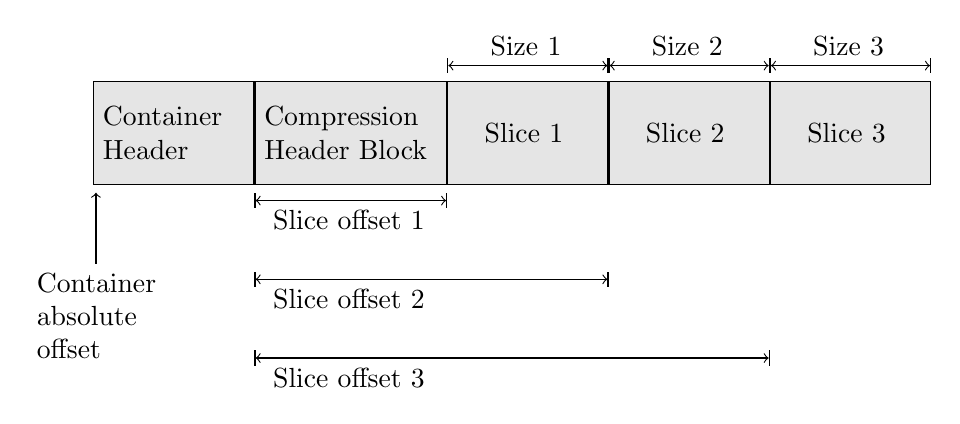
\begin{tikzpicture}[
  boxed/.style={rectangle, draw=black, fill=black!10, minimum height=1.3cm, text width=1.8cm},
]
\node(A) [boxed]{Container Header};
\node(B) [boxed,right,text width=2.2cm] at (A.east){Compression Header Block};
\node(C) [boxed,right] at (B.east){\quad Slice 1};
\node(D) [boxed,right] at (C.east){\quad Slice 2};
\node(E) [boxed,right] at (D.east){\quad Slice 3};

\draw[<-] (A.south west)+(1pt,-0.1cm) -- +(1pt,-1cm)
     node[below, text width=1.5cm]{Container absolute offset};


\draw[|<->|] ([yshift=-0.2cm]B.south west) node[below,xshift=1.2cm]{Slice offset 1}
    -- ([yshift=-0.2cm]B.south east);
\draw[|<->|] ([yshift=-1.2cm]B.south west) node[below,xshift=1.2cm]{Slice offset 2}
    -- ([yshift=-1.2cm]C.south east);
\draw[|<->|] ([yshift=-2.2cm]B.south west) node[below,xshift=1.2cm]{Slice offset 3}
    -- ([yshift=-2.2cm]D.south east);

\draw[|<->|] ([yshift=+0.2cm]C.north west) node[above,xshift=1cm]{Size 1} -- ([yshift=+0.2cm]C.north east);
\draw[|<->|] ([yshift=+0.2cm]D.north west) node[above,xshift=1cm]{Size 2} -- ([yshift=+0.2cm]D.north east);
\draw[|<->|] ([yshift=+0.2cm]E.north west) node[above,xshift=1cm]{Size 3} -- ([yshift=+0.2cm]E.north east);


\end{tikzpicture}
\end{center}

\subsubsection*{BAM index}

BAM indexes are supported by using 4-byte integer pointers called landmarks that 
are stored in container header. BAM index pointer is a 64-bit value with 48 bits 
reserved for the BAM block start position and 16 bits reserved for the in-block 
offset. When used to index CRAM files, the first 48 bits are used to store the 
CRAM container start position and the last 16 bits are used to store the index 
of the landmark in the landmark array stored in  container header. The landmark 
index can be used to access the appropriate slice. 

The above indexing scheme treats CRAM slices as individual records in BAM file. 
This allows to apply BAM indexing to CRAM files, however it introduces some overhead 
in seeking specific alignment start because all preceding records in the slice 
must be read and discarded.

\section{Encodings}
\label{sec:encodings}

% FIXME: we have a mishash of coding, encoding and codec.  We should
% go through the entire document and be consistent.

\subsection{Introduction}

The basic idea for encodings is to efficiently represent byte and integer values.
This can be achieved in a number of ways that most frequently involve some knowledge 
about the nature of the values being encoded, for example, distribution statistics. 
The methods for choosing the best encoding and determining its parameters are very 
diverse and are not part of the CRAM format specification, which only describes 
how the information needed to decode the values should be stored.

\subsection{BYTE}

This encoding simply stores byte values verbatim to a block with a given ID.

\subsubsection*{Parameters}

CRAM format defines the following parameters for BYTE encoding: 

\begin{tabular}{|>{\raggedright}p{100pt}|>{\raggedright}p{100pt}|>{\raggedright}p{230pt}|}
\hline
\textbf{Data type} & \textbf{Name} & \textbf{Comment}
\tabularnewline
\hline
uint7 & id & id of a block containing the byte stream\tabularnewline
\hline
\end{tabular}

\subsection{VARINT\_UNSIGNED}

This encoding stores unsigned integer values using the Variable Length Quantity
format (VLQ)\footnote{https://en.wikipedia.org/wiki/Variable-length\_quantity}.

It is not permitted to store any negative values using this encoding.
However given several data series have ranges that have the
possibility of small negative values (such as -1 for Alignment
Position), it is possible to skew the values slightly by adding an
offset prior to encoding.  This provides a mechanism for guaranteeing
all values remain positive.

Note this offset is added to the value after that value has been
decoded so to encode -1 we may wish to set offset to -1 and encode a
zero.  This mechanism may also be used to skew a range of values that
do not cluster around zero.  For example if a data series has values
ranging from 1000 to 1200, then setting offset to 1000 and encoding
values between 0 and 200 would provide a smaller data footprint.

For data series that require a broader scope of signed values we would
recommend using VARINT\_SIGNED instead.

\subsubsection*{Parameters}

CRAM format defines the following parameters for VARINT\_UNSIGNED encoding: 

\begin{tabular}{|>{\raggedright}p{100pt}|>{\raggedright}p{100pt}|>{\raggedright}p{230pt}|}
\hline
\textbf{Data type} & \textbf{Name} & \textbf{Comment}
\tabularnewline
\hline
sint7 & offset & amount to add to decoded values\tabularnewline
\hline
uint7 & id & id of a block containing the byte stream\tabularnewline
\hline
\end{tabular}

\subsection{VARINT\_SIGNED}

This encoding permits storing a broad range of both positive and
negative values while still following the property of low magnitude
values taking up less space than large magnitude ones.

It achieves this by using ZigZag encoding where signed values 0, -1,
+1, -2, +2 and so on are mapped to unsigned values 0, 1, 2, 3, 4.
These unsigned values are then stored using the same VLQ system used
by VARINT\_UNSIGNED.

As with VARINT\_UNSIGNED, an offset is added to the value after it has
been VLQ and ZigZag decoded.  Combined these permit efficient storage
of a distribution of values centred around a mean.  For example if
the distribution of values in a data series ranged from 1000 to 2000
with a peak at 1500, we could set offset to 1500 and encode values
-500 to +500.

\subsubsection*{Parameters}

CRAM format defines the following parameters for VARINT\_SIGNED encoding: 

\begin{tabular}{|>{\raggedright}p{100pt}|>{\raggedright}p{100pt}|>{\raggedright}p{230pt}|}
\hline
\textbf{Data type} & \textbf{Name} & \textbf{Comment}
\tabularnewline
\hline
sint7 & offset & amount to add to decoded values\tabularnewline
\hline
uint7 & id & id of a block containing the byte stream\tabularnewline
\hline
\end{tabular}


\subsection{CONST\_BYTE}

Sometimes a data series has a constant value throughout the
container.  In this case we can record this value in the Container
Compression Header and avoid the need to store the data series.

\subsubsection*{Parameters}

CRAM format defines the following parameters for CONST\_BYTE encoding: 

\begin{tabular}{|>{\raggedright}p{100pt}|>{\raggedright}p{100pt}|>{\raggedright}p{230pt}|}
\hline
\textbf{Data type} & \textbf{Name} & \textbf{Comment}
\tabularnewline
\hline
byte & value & the constant value\tabularnewline
\hline
\end{tabular}

\subsection{CONST\_INT}

As per CONST\_BYTE, but the value is a signed integer encoded with
VLQ and ZigZag methods.
The overhead of using ZigZag encoding on a constant unsigned value is
an average of 1 bit per container per use of this encoding.

\subsubsection*{Parameters}

CRAM format defines the following parameters for CONST\_INT encoding: 

\begin{tabular}{|>{\raggedright}p{100pt}|>{\raggedright}p{100pt}|>{\raggedright}p{230pt}|}
\hline
\textbf{Data type} & \textbf{Name} & \textbf{Comment}
\tabularnewline
\hline
sint & value & the constant value\tabularnewline
\hline
\end{tabular}

\subsection{BYTE\_ARRAY\_LEN (ID 4)}

Can encode types \textit{Byte[]}.

Often there is a need to encode an array of bytes where the length is
not predetermined.  For example the read identifiers differ per
alignment record, possibly with different lengths, and this length
must be stored somewhere.   Note in contrast to this, quality values
are known to be the same length as the sequence which is an already
known quantity, so the CRAM record encodes this using an implicit
array by asking for multiple values to be decoded rather than using an
explicit byte array encoding.

With BYTE\_ARRAY\_LEN the length is explicitly encoded via its own
sub-encoding prior to the array of bytes itself, also via its own
sub-encoding.

Note these sub-encodings may store the data in the same block, in
which case the length comes first. Alternatively we may decide that
the lengths have their own unique distribution which differs
substantially to the data itself and so should be stored in a
different block to permit better compression.  Having decoded the
length, the decoder must then call the value sub-encoding that many
times to retrieve the bytes.

Given the recursion used here of an encoding using two sub-encodings,
the byte stream for BYTE\_ARRAY\_LEN is the concatenation of both
sub-encodings.

\subsubsection*{Parameters}

The parameters for BYTE\_ARRAY\_LEN are listed below:

\begin{tabular}{|>{\raggedright}p{100pt}|>{\raggedright}p{100pt}|>{\raggedright}p{230pt}|}
\hline
\textbf{Data type} & \textbf{Name} & \textbf{Comment}
\tabularnewline
\hline
encoding\texttt{<}int\texttt{>} & lengths encoding & an encoding describing how 
the arrays lengths are stored\tabularnewline
\hline
encoding\texttt{<}byte\texttt{>} & values encoding & an encoding describing how 
the values (bytes) are stored\tabularnewline
\hline
\end{tabular}

\subsubsection*{Example}

The bytes for an X0:i SAM auxiliary field consisting of 16-bit items
may be written as an X0S tag line.  Despite the size being known, all
tag items are stored as byte arrays, so BYTE\_ARRAY\_LEN is ideal when
coupled with a CONST\_INT encoding to hold the fixed size lengths and
BYTE for the values.

\begin{tabular}{lll}
\hline
\textbf{Bytes} & & \textbf{Meaning}\\
\hline
\texttt{0x04}         & & BYTE\_ARRAY\_LEN encoding ID                                    \\
\texttt{0x07}         & & 7 remaining bytes of BYTE\_ARRAY\_LEN parameters            \\
\\
\texttt{0x44}         & & CONST\_INT encodng ID, for the aux tag lengths \\
\texttt{0x01}         & & remaining length of CONST\_INT encoding \\
\texttt{0x05}         & & length 2 as Zig-Zag format \\
\\
\texttt{0x01}         & & BYTE encoding ID, for the aux tag values \\
\texttt{0x02}         & & 2 more bytes of BYTE parameters                          \\
\texttt{0x81 0x48}    & & uint7 encoding for block ID 200                              \\
\hline
\end{tabular}

\subsection{BYTE\_ARRAY\_STOP (ID 5)}

Can encode types \textit{Byte[]}.

Instead of encoding an explicit length (as per BYTE\_ARRAY\_LEN) this
encoding stores bytes ending in a termination value.  The data
returned should not include this termination byte.  Hence this is
comparable to the C language string encoding, which uses a nul
character for termination, while BYTE\_ARRAY\_LEN is more similar to
the Pascal language string encoding.

Given this encoding is capturing the length within the same data
stream as the bytes, unlike BYTE\_ARRAY\_LEN this does not require
use of sub-encodings.  This makes it considerably simpler, but it has
redundancy when the stored arrays have constant lengths.

The choice of termination symbol is up to the encoder, but logical
choices may include the nul byte or the tab character as both are
illegal within SAM records.

\begin{tabular}{|>{\raggedright}p{100pt}|>{\raggedright}p{100pt}|>{\raggedright}p{230pt}|}
\hline
\textbf{Data type} & \textbf{Name} & \textbf{Comment}
\tabularnewline
\hline
byte & stop byte & a special byte treated as a delimiter\tabularnewline
\hline
uint7 & block id & id of a block containing the byte stream\tabularnewline
\hline
\end{tabular}

% \subsection{Beta coding: codec ID 6}
% 
% Can encode types \textit{Integer}.
% 
% \subsubsection*{Definition}
% 
% Beta coding is a most common way to represent numbers in \emph{binary notation} and is sometimes referred to as binary coding.
% The decoder reads the specified fixed number of bits (most significant first) and subtracts the offset value to get the decoded integer.
% 
% \subsubsection*{Parameters}
% 
% CRAM format defines the following parameters of beta coding: 
% 
% \begin{tabular}{|>{\raggedright}p{144pt}|>{\raggedright}p{144pt}|>{\raggedright}p{144pt}|}
% \hline
% \textbf{Data type} & \textbf{Name} & \textbf{Comment}\tabularnewline
% \hline
% itf8 & offset & offset is subtracted from each value during decode\tabularnewline
% \hline
% itf8 & length & the number of bits used\tabularnewline
% \hline
% \end{tabular}
% 
% \subsubsection*{Examples}
% 
% If we have integer values in the range 10 to 15 inclusive, the largest value would traditionally need 4 bits, but with an offset of -10 we can hold values 0 to 5, using a fixed size of 3 bits.
% Using fixed Offset and Length coming from the beta parameters, we decode these values as:
% 
% \begin{tabular}{|>{\raggedright}p{105pt}|>{\raggedright}p{105pt}|>{\raggedright}p{105pt}|>{\raggedright}p{105pt}|}
% \hline
% Offset & Length & \textbf{Bits} & \textbf{Value}\tabularnewline
% \hline
% -10 & 3 & 000 & 10\tabularnewline
% \hline
% -10 & 3 & 001 & 11\tabularnewline
% \hline
% -10 & 3 & 010 & 12\tabularnewline
% \hline
% -10 & 3 & 011 & 13\tabularnewline
% \hline
% -10 & 3 & 100 & 14\tabularnewline
% \hline
% -10 & 3 & 101 & 15\tabularnewline
% \hline
% \end{tabular}
% 
% \subsection{Subexponential coding: codec ID 7}
% 
% Can encode types \textit{Integer}.
% 
% \subsubsection*{Definition}
% 
% Subexponential coding\footnote{Fast progressive lossless image compression, Paul G. Howard and Jeffrey Scott Vitter, 1994. \url{http://www.ittc.ku.edu/~jsv/Papers/HoV94.progressive_FELICS.pdf}} is parametrized by a non-negative integer $k$.
% For values $n < 2^{k+1}$ subexponential coding produces codewords identical to Rice coding \footnote{\url{https://en.wikipedia.org/wiki/Golomb_coding\#Rice_coding}}.  For larger values it grows logarithmically with $n$.
% 
% \subsubsection*{Encoding}
% 
% \begin{enumerate}
% \item Add $\mathit{offset}$ to $n$.
% 
% \item Determine $u$ and $b$ values from $n$
% \begin{align*}
% b =
% \begin{cases}
%   \ k                        & \text{ if $n < 2^k$} \\
%   \ \lfloor log_{2}n \rfloor & \text{ if $n \ge 2^k$}
% \end{cases}
% &\
% &u =
% \begin{cases}
%   \ 0     & \text{ if $n < 2^k$} \\
%   \ b-k+1 & \text{ if $n \ge 2^k$}
% \end{cases}
% \end{align*}
% 
% \item Write $u$ in unary form; $u$ 1 bits followed by a single 0 bit.
% 
% \item Write the bottom $b$-bits of $n$ in binary form.
% \end{enumerate}
% 
% \subsubsection*{Decoding}
% 
% \begin{enumerate}
% \item Read $u$ in unary form, counting the number of leading 1s (prefix) in the codeword (discard the trailing 0 bit).
% 
% \item Determine $n$ via:
% \begin{enumerate}
% \item if $u = 0$ then read $n$ as a $k$-bit binary number.
% \item if $u \ge 1$ then read $x$ as a $(u + k - 1)$-bit binary. Let $n = 2^{u+k-1} + x$.
% \end{enumerate}
% 
% \item Subtract $\mathit{offset}$ from $n$.
% \end{enumerate}
% 
% \subsubsection*{Examples}
% 
% \begin{tabular}{|>{\raggedright}p{105pt}|>{\raggedright}p{105pt}|>{\raggedright}p{105pt}|>{\raggedright}p{105pt}|}
% \hline
% \textbf{Number} & \textbf{Codeword, k=0} & \textbf{Codeword, k=1} & \textbf{Codeword, 
% k=2}\tabularnewline
% \hline
% 0 & 0 & 00 & 000\tabularnewline
% \hline
% 1 & 10 & 01 & 001\tabularnewline
% \hline
% 2 & 1100 & 100 & 010\tabularnewline
% \hline
% 3 & 1101 & 101 & 011\tabularnewline
% \hline
% 4 & 111000 & 11000 & 1000\tabularnewline
% \hline
% 5 & 111001 & 11001 & 1001\tabularnewline
% \hline
% 6 & 111010 & 11010 & 1010\tabularnewline
% \hline
% 7 & 111011 & 11011 & 1011\tabularnewline
% \hline
% 8 & 11110000 & 1110000 & 110000\tabularnewline
% \hline
% 9 & 11110001 & 1110001 & 110001\tabularnewline
% \hline
% 10 & 11110010 & 1110010 & 110010\tabularnewline
% \hline
% \end{tabular}
% 
% \subsubsection*{Parameters}
% 
% \begin{tabular}{|>{\raggedright}p{100pt}|>{\raggedright}p{100pt}|>{\raggedright}p{230pt}|}
% \hline
% \textbf{Data type} & \textbf{Name} & \textbf{Comment}
% \tabularnewline
% \hline
% itf8 & offset & offset is subtracted from each value during decode\tabularnewline
% \hline
% itf8 & k & the order of the subexponential coding\tabularnewline
% \hline
% \end{tabular}
% 
% \subsection{Gamma coding: codec ID 9}
% 
% Can encode types \textit{Integer}.
% 
% \subsubsection*{Definition}
% 
% \emph{Elias gamma code} is a prefix encoding of positive integers. This is a combination 
% of unary coding and beta coding. The first is used to capture the number of bits 
% required for beta coding to capture the value. 
% 
% \subsubsection*{Encoding}
% 
% \begin{enumerate}
% \item Write it in binary.
% 
% \item Subtract $1$ from the number of bits written in step 1 and prepend that many zeros.
% 
% \item An equivalent way to express the same process:
% 
% \item Separate the integer into the highest power of $2$ it contains ($2N$) and the remaining 
% $N$ binary digits of the integer.
% 
% \item Encode $N$ in unary; that is, as $N$ zeroes followed by a one.
% 
% \item Append the remaining $N$ binary digits to this representation of $N$.
% \end{enumerate}
% 
% \subsubsection*{Decoding}
% 
% \begin{enumerate}
% \item Read and count 0s from the stream until you reach the first 1. Call this count 
% of zeroes $N$.
% 
% \item Considering the one that was reached to be the first digit of the integer, with 
% a value of $2N$, read the remaining $N$ digits of the integer.
% \end{enumerate}
% 
% \subsubsection*{Examples}
% 
% \begin{tabular}{|>{\raggedright}p{76pt}|>{\raggedright}p{107pt}|}
% \hline
% \textbf{Value} & \textbf{Codeword}\tabularnewline
% \hline
% 1 & 1\tabularnewline
% \hline
% 2 & 010\tabularnewline
% \hline
% 3 & 011\tabularnewline
% \hline
% 4 & 00100\tabularnewline
% \hline
% \end{tabular}
% 
% \subsubsection*{Parameters}
% 
% \begin{tabular}{|>{\raggedright}p{144pt}|>{\raggedright}p{144pt}|>{\raggedright}p{144pt}|}
% \hline
% \textbf{Data type} & \textbf{Name} & \textbf{Comment}\tabularnewline
% \hline
% itf8 & offset & offset to subtract from each value after decode\tabularnewline
% \hline
% \end{tabular}
% 
% \subsection{DEPRECATED: Golomb coding: codec ID 2}
% 
% Can encode types \textit{Integer}.
% 
% Note this codec has not been used in any known CRAM implementation since before CRAM v1.0.
% Nor is it implemented in some of the major software.
% Therefore its use is not recommended.
% 
% \subsubsection*{Definition}
% 
% \emph{Golomb encoding} is a prefix encoding optimal for representation of random 
% positive numbers following geometric distribution. 
% 
% \subsubsection*{Encoding}
% 
% \begin{enumerate}
% \item Fix the parameter $M$ to an integer value.
% 
% \item For $N$, the number to be encoded, find
% 
% \begin{enumerate}
% \item quotient $q = \lfloor N/M \rfloor$
% 
% \item remainder $r = N \bmod M$
% \end{enumerate}
% 
% \item Generate Codeword
% 
% \begin{enumerate}
% \item The Code format : \texttt{<}Quotient Code\texttt{>}\texttt{<}Remainder Code\texttt{>}, 
% where
% 
% \item Quotient Code (in unary coding)
% 
% \begin{enumerate}
% \item Write a $q$-length string of 1 bits
% 
% \item Write a 0 bit
% \end{enumerate}
% 
% \item Remainder Code (in truncated binary encoding)
% 
% Set $b=\lceil log_{2}(M) \rceil$
% 
% \begin{enumerate}
% \item If $r < 2^{b}-M$ code $r$ as plain binary using $b-1$ bits.
% 
% \item If $r \ge 2^{b}-M$ code the number $r+2^{b}-M$ in plain binary representation 
% using $b$ bits.
% \end{enumerate}
% \end{enumerate}
% \end{enumerate}
% 
% \subsubsection*{Decoding}
% 
% \begin{enumerate}
% \item Read $q$ via unary coding: count the number of 1 bits and consume the following 0 bits.
% \item Set $b=\lceil log_{2}(M) \rceil$
% \item Read $r$ via $b-1$ bits of binary coding
% \item If $r \ge 2^{b}-M$
% \begin{enumerate}
% \item Read 1 single bit, $x$.
% \item Set $r = r*2 + x - (2^{b}-M)$
% \end{enumerate}
% \item Value is $q*M + r - \mathit{offset}$
% \end{enumerate}
% 
% \subsubsection*{Examples}
% 
% \begin{tabular}{|>{\raggedright}p{76pt}|>{\raggedright}p{107pt}|}
% \hline
% \textbf{Number} & \textbf{Codeword, M=10, (thus b=4)}\tabularnewline
% \hline
% 0 & 0000\tabularnewline
% \hline
% 4 & 0100\tabularnewline
% \hline
% 10 & 10000\tabularnewline
% \hline
% 26 & 1101100\tabularnewline
% \hline
% 42 & 11110010\tabularnewline
% \hline
% \end{tabular}
% 
% \subsubsection*{Parameters}
% 
% Golomb coding takes the following parameters: 
% 
% \begin{tabular}{|>{\raggedright}p{144pt}|>{\raggedright}p{144pt}|>{\raggedright}p{144pt}|}
% \hline
% \textbf{Data type} & \textbf{Name} & \textbf{Comment}\tabularnewline
% \hline
% itf8 & offset & offset is added to each value\tabularnewline
% \hline
% itf8 & M & the golomb parameter (number of bins)\tabularnewline
% \hline
% \end{tabular}
% 
% \subsection{DEPRECATED: Golomb-Rice coding: codec ID 8}
% 
% Can encode types \textit{Integer}.
% 
% Note this codec has not been used in any known CRAM implementation since before CRAM v1.0.
% Nor is it implemented in some of the major software.
% Therefore its use is not recommended.
% 
% Golomb-Rice coding is a special case of Golomb coding when the M parameter is a power of 2.
% The reason for this coding is that the division operations in Golomb coding can be replaced with bit shift operators as well as avoiding the extra $r < 2^{b}-M$ check.

\section{Block compression methods}

Each block will hold different types of data and may have very
different characteristics for compression.  Hence CRAM can utilise
several different compression methods. Each method has an associated numeric code which is defined in Section~\ref{sec:block-struct}.

The following methods are defined.
Exact definitions of these methods are in their respective internet links or the ancillary \textit{CRAMcodecs} document found along side this specification.

\subsection{Gzip}

The Gzip specification is defined in RFC 1952.
Gzip in turn is an encapsulation on the Deflate algorithm defined in RFC 1951.

\subsection{Bzip2}

First available in CRAM v2.0.

Bzip2 is a compression method utilising the Burrows Wheeler Transform, Move To Front transform, Run Length Encoding and a Huffman entropy encoder. 
It is often superior to Gzip for textual data.

An informal format specification exists:\\
\url{https://github.com/dsnet/compress/blob/master/doc/bzip2-format.pdf}

\subsection{LZMA}

First available in CRAM v3.0.

LZMA is the Lempel-Ziv Markov chain algorithm.
CRAM uses the xz Stream format to encapsulate this algorithm, as defined in \url{https://tukaani.org/xz/xz-file-format.txt}.

\subsection{rANS4x8 codec}

First available in CRAM v3.0.

rANS is the range-coder variant of the Asymmetric Numerical
System\footnote{J. Duda, \textit{Asymmetric numeral systems: entropy
    coding combining speed of Huffman coding with compression rate of
    arithmetic coding}, \url{http://arxiv.org/abs/1311.2540}}.

``4x8'' refers to 4-way interleaving with 8-bit renormalisation.\newline
This variant of rANS first appeared in CRAM v3.0.

Details of this algorithm have been moved to the \textit{CRAMcodecs} document.

\subsection{rANS4x16 codec}

First available in CRAM v3.1.

``4x16'' refers to 4-way interleaving with 16-bit renormalisation.\newline
This variant of rANS first appeared in CRAM v3.1.

Details of this algorithm are listed in the \textit{CRAMcodecs} document.

\subsection{adaptive arithemtic coding}

First available in CRAM v3.1.

An entropy encoder that is slower but slightly more concise than
rANS.  It achieves this by adapting the probabilities as it compresses
and decompresses instead of using a fixed table.

Details of this algorithm are listed in the \textit{CRAMcodecs} document.

\subsection{fqzcomp codec}

First available in CRAM v3.1.

This is a method dedicated to compression of quality values.

Details of this algorithm are listed in the \textit{CRAMcodecs} document.

\subsection{name tokeniser}

First available in CRAM v3.1.

This is a method dedicated to compression of read names.

Details of this algorithm are listed in the \textit{CRAMcodecs} document.

\appendix
\renewcommand{\thesection}{\arabic{section}}

\newcommand{\appsection}[1]{%
  \addtocounter{section}{1}
  \section*{Appendix~\thesection \quad #1}
  \addcontentsline{toc}{section}{Appendix~\thesection \quad #1}
}

\appsection{Choosing the container size}

The CRAM format does not constrain the size of the containers.
However, the following should be considered when deciding the container size:

-- Data can be compressed better by using larger containers.

-- Random access performance is better for smaller containers.

-- Streaming is more convenient for small containers.

-- Applications typically buffer containers into memory.

-- Multi-threaded applications likely have a granularity of 1
container for each unit of work.

As a guidance, the default container size for htslib and htsjdk is one
slice of 10,000 short reads (fewer for long reads), but some users
find 1,000 is more appropriate if they need a lot of random access.

\appsection{CRAM 4.0 changes and rationale}
\label{sec:cram4changes}

CRAM 4.0 has a number of changes.  For those familier with the version
3.0 format, this is a list of changes along with a rationale for
making them.

\begin{description}
\item[New variable sized integer encoding]\ \newline
  Use VLQ (https://en.wikipedia.org/wiki/Variable-length\_quantity)
  instead of ITF8 and LTF8.

  This has the impact of not needing to distinguish between 32-bit and
  64-bit quantities, which we previously needed to do with ITF8 vs
  LTF8.  It also has a small reduction to compressed sizes.


\item[Long chromosome support]\ \newline
  A corollary of the removal of ITF8 and LTF8 means all fields
  can now be 64-bit if appropriate.  Importantly this removes the
  32-bit limit on the size of AP (alignment pos), TS (template size),
  NP (next mate pos).


\item[Signed numbers]\ \newline
  Variable sized integer encoding can now also do signed numbers.
  Previously -1 was stored as FF FF FF 0F (ITF8) and even more FFs
  for LTF8.  This is unwieldy and also bakes in knowledge of the
  size of the intended data type, making it impossible to increase
  data type sizes without changing the format.

  Signed fields are used for AP (alignment pos), TS (template size)
  and RG (read group, which can be -1 for not present).


\item[MD, NM presence and location]\ \newline
  CRAM derives MD and NM tags on-the-fly where possible.  However it
  doesn't record whether they were in the original data.

  The presence of MD and NM are now recorded, so if the input data didn't
  have them we won't reproduce on decode, and vice versa.  The
  location of MD, NM and RG in the tag stream are now also recorded,
  meaning CRAM 4.0 will round-trip more precisely.


\item[Quality value orientation]\ \newline
  On some technologies it is better to record qualities in their
  original orientation rather than the alignment orientation as this
  improves compression ratios.

  This is an optional setting in the compression header.  The data
  should be automatically flipped back during decode so the operation
  is transparent to the user.


\item[New CF explicit template size flag]\ \newline
  In CRAM RNEXT, PNEXT and TLEN are generated on-the-fly for read
  pairs residing in the same slice.  If we wish to preserve data
  verbatim for exceptions, such as TLEN off-by-one errors (common in
  old data) or TLEN 5' to 5' vs leftmost to rightmost differences then
  we had to mark the record as ``detached'' and store all 3 fields.

  We now have an flag to state that TLEN is explicitly stored without
  needing to use the CF detached flag.  This can have a substantial
  impact on file sizes for some older data sets.


\item[Deduplication of read names]\ \newline
  For read pairs residing in the same slice we can use the same logic
  we previously used for RNEXT, PNEXT and TLEN generation to also
  deduplicate read names so it only needs storing once.

  This roughly halves the size of uncompressed RN data series,
  reducing the compressed size.

{\color{gray}
\item[(For consideration) Removal of slices]\ \newline
  CRAM 3.0 offers the ability to have multiple slices per container.
  
  This is largely unused and does not provide the originally planned
  benefits of sharing compression meta-data between slices.  The
  defaults from both htslib and htsjdk are one slice per container.

  Removal of multi-slice containers, and by extension slices
  themselves, offers a simplified interface.

  An alternative to this is to permit another set of blocks prior to
  the first slice, with duplicate block IDs to those used in the
  slices.  These blocks pertain to the container and are utilised in
  unison with the per slice blocks.  For rANS they could hold the
  frequency tables, permitting this to be shared across slices.  For
  gzip or zstd they could hold a predefined dictionary, permitting
  more efficient compression of small blocks.  This may grant finer
  grained random access capability without suffering so much data
  expansion.
}

\item[TODO: add PACK, RLE and DELTA encodings]\ \newline

\item[TODO: sanitize read\_names\_included]\ \newline
  Given we now state a blank name will copy from the mate pair and
  auto-generate if not, there's no need for this field.  We can just
  store blank names and cull the whole RN in DecodeMateData vs in-line
  shenanigans.

\item[TODO: make all aux tags first class encoding objects]\ \newline
  Right now aux tags are basically byte arrays encoded as per BAM.
  This isn't so efficient.  For example an XX:S data series with
  values ranging 0 to 500 but with many more small values are a few
  large ones would be better encoded as VLQ than an array of 16-bit
  quantities.

\end{description}

\end{document}

\title{CRAM format specification (version 4.0)}
\author{samtools-devel@lists.sourceforge.net}
\date{\headdate}
\maketitle


\begin{quote}\small
The master version of this document can be found at
\url{https://github.com/samtools/hts-specs}.\\
This printing is version~\commitdesc\ from that repository,
last modified on the date shown above.
\end{quote}

\begin{center}
\textit{license: Apache 2.0}
\end{center}
\vspace*{1em}

\tableofcontents
\newpage

\section{Overview}

This specification describes the CRAM 4.0 format. 

CRAM has the following major objectives:

\begin{enumerate}
\item Significantly better lossless compression than BAM

\item Full compatibility with BAM

\item Effortless transition to CRAM from using BAM files

\item Support for controlled loss of BAM data
\end{enumerate}

The first three objectives allow users to take immediate advantage of the CRAM 
format while offering a smooth transition path from using BAM files. The fourth 
objective supports the exploration of different lossy compression strategies and 
provides a framework in which to effect these choices. Please note that the CRAM 
format does not impose any rules about what data should or should not be preserved. 

Data in CRAM is aggregated by data type (analogous to SAM columns)
known as Data Series and stored in blocks with each block compressed
using a choice of general purpose or custom compression codecs.
Sequence is typically encoded relative to a reference
sequence\footnote{Markus Hsi-Yang Fritz, Rasko Leinonen, Guy Cochrane,
  and Ewan Birney, \textbf{Efficient storage of high throughput DNA
    sequencing data using reference-based compression}, {\sl Genome
    Res.}~2011~21: 734--740;
  \href{http://dx.doi.org/doi:10.1101/gr.114819.110}{doi:10.1101/gr.114819.110};
  {\sc pmid:}21245279.}, but this is not a requirement.  Both aligned
and unaligned sequence is supported.

\section{Data types and formats}
\subsection*{Structures}

The CRAM format consists of header structures (container, compression, slice and block) and data series stored within the blocks themselves.
The fields of these structures use a mixture of fundamental types - boolean, byte, integer or array thereof - which are defined below.

% Types used in structures.
% Container:  uint, sint, uint[], byte[4](CRC), byte[]
% Block:      byte, uint, byte[], byte[4](CRC)
% CompHdr:    map, bool, byte[5], uint, byte[], encoding<>
% Slice:      sint, uint, uint[], byte[16], byte[]

\begin{tabular}{lll}
\textbf{Field type}  & \textbf{Format} & \textbf{Description}\\
\textit{bool}  & \textbf{byte} & A boolean, 0 (false) or 1 (true), stored as a byte. \\
\textit{byte}  & \textbf{byte} & An unsigned single byte (8 bits)  \\
\textit{uint}  & \textbf{VLQ\_unsigned} & A variable length integer $x >= 0$\\
\textit{sint}  & \textbf{VLQ\_signed}   & A variable length integer (may be negative)\\
\textit{array\texttt{<}type\texttt{>}} & \textbf{array} & An array of items of \textit{type} including the dimension\\
\\
\textit{type[]}  & \textit{as appropriate} & Zero or more items with unspecified length\\
\textit{type[4]} & \textit{as appropriate} & A constant number of items, dimension not stored\\
\end{tabular}
\vskip 10pt

The on-disk format for each of these encodings is listed below:

\begin{description}
\item[\textbf{byte}]\ \newline
A single byte

\item[\textbf{VLQ\_unsigned}]\ \newline
Integer values are encoded using Variable Length
Quantity\footnote{\url{https://en.wikipedia.org/wiki/Variable-length_quantity}}.

If the value is larger than 7-bits then the top-bit of the byte is
set, indicating a subsequent byte must be read.  This is repeated
until the top bit is unset. Bytes are written with the most
significant values first (big-endian format), which simplifies the
decode process.

Algorithmically this looks like:

\begin{algorithmic}[1]
\Statex
\Statex \textit{Read a variable sized unsigned integer 7-bits at a time.}
\Function{ReadUint7}{}
  \State $value \gets 0$
  \Repeat
    \State $c \gets$ \Call{ReadUint8}{}
    \State $value \gets (value \shiftl 7) + (c \bitand 127)$
  \Until{$c < 128$}
  \State \Return $value$
  \EndFunction
\end{algorithmic}

\item[\textbf{VLQ\_unsigned}]\ \newline
Signed integers are initially transformed to unsigned values using a zig-zag transformation, and then encoded as per unsigned values.
This maps signed values 0, -1, +1, -2, +2 to unsigned values 0, 1, 2, 3, 4 respectively, and vice versa during decode.

The zig-zag encoding method involves shifting the value left 1
bit and then XORing with all-bits-zero if positive or all-bits-one if
negative. I.e. $(v \shiftl 1) \bitxor (v \shiftr 31)$ for a
32-bit quantity using a 2's complement arithmetic shift right.

Decoding a zig-zag value is similar.  We XOR the value shifted right 1
bit with 0 or -1, taken from the negation of the bottom bit, as seen
below.

\begin{algorithmic}[1]
\Statex
\Statex \textit{Read a variable sized signed integer 7-bits at a time.}
\Function{ReadSint7}{}
  \State $value \gets $ \Call{ReadUint7}{}
  \State \Return $(value \shiftr 1) \bitxor -(value \bitand 1)$
  \EndFunction
\end{algorithmic}

\item[\textbf{array}]\ \newline
An array of items with the array dimension explicitly stored.
The array dimension is first, using VLQ\_signed format, followed by the array elements stored as per their \textit{type}.

\end{description}

Other custom data types exist, but will be introduced in the relevant sections.

\section{File Layout}

The basic structure of a CRAM file is a file header (magic number)
followed by a series of containers.  The first of these containers
holds textual meta-data (CRAM Header Container) and the last is used
as an end-of-file marker (CRAM EOF Container) with everyone inbetween
holding the sequence records themselves (Data Contaners).

\begin{center}
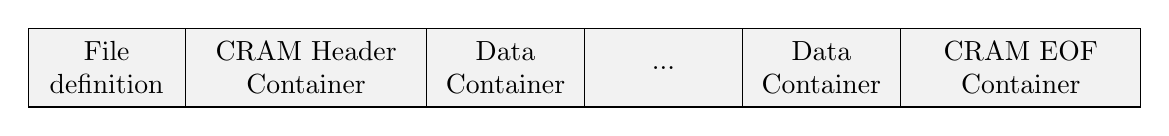
\begin{tikzpicture}[
  every node/.style={scale=1.0},
  boxes/.style={rectangle split,rectangle split parts=#1,draw,rectangle split horizontal,text width=5em,align=center,minimum height=1cm,fill=black!5,on grid},
  notes/.style={text width=20em,align=center,minimum height=1cm,on grid},
]
\node (file) [boxes=6] {
\nodepart{one}File definition
\nodepart[text width=8em]{two}CRAM Header Container
\nodepart{three}Data Container
\nodepart{four}...
\nodepart{five}Data Container
\nodepart[text width=8em]{six}CRAM EOF Container
};
\end{tikzpicture}

Figure 1: A CRAM file consists of a file definition, followed by a header container, then other containers.
\end{center}

Containers are just a Container Header Structure followed by one or
more Blocks.  Blocks have different types (see
~\ref{subsec:block-content-types}) corresponding to their usage.
Note the block itself also consists of a defined structure followed by
the block contents data.

\begin{center}
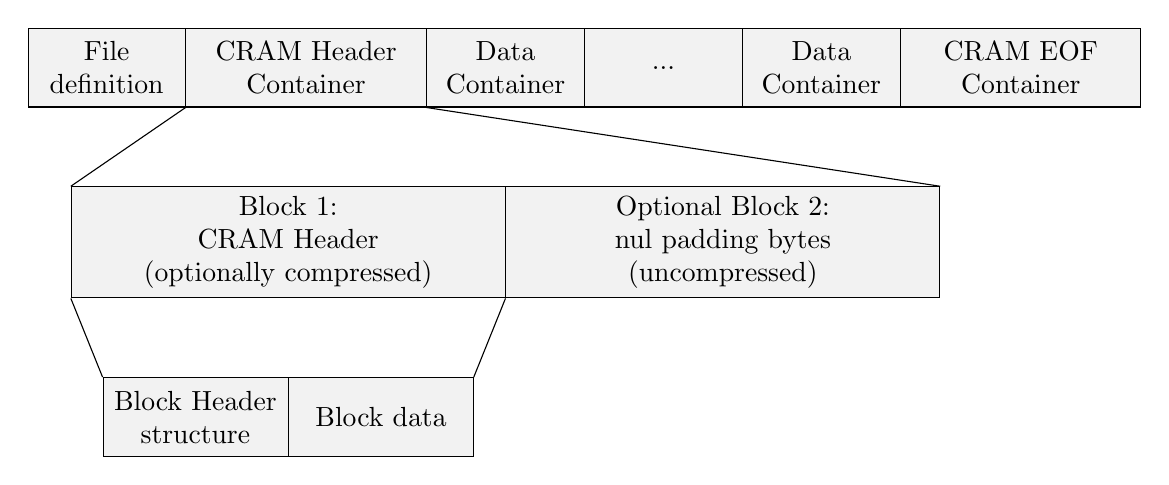
\begin{tikzpicture}[
  every node/.style={scale=1.0},
  boxes/.style={rectangle split,rectangle split parts=#1,draw,rectangle split horizontal,text width=5em,align=center,minimum height=1cm,fill=black!5,on grid},
  notes/.style={text width=20em,align=center,minimum height=1cm,on grid},
]
\node (file) [boxes=6] {
\nodepart{one}File definition
\nodepart[text width=8em]{two}CRAM Header Container
\nodepart{three}Data Container
\nodepart{four}...
\nodepart{five}Data Container
\nodepart[text width=8em]{six}CRAM EOF Container
};

\node (header) [boxes=2,below=1 of file.three south, text width=15em] {
\nodepart{one}Block 1:\break
CRAM Header\break
(optionally compressed)
\nodepart{two}Optional Block 2:\break
nul padding bytes\break
(uncompressed)
};
\draw (file.one split south) to (header.north west);
\draw (file.two split south) to (header.north east);

\node (blocks) [boxes=2,below=1 of header.one south,text width=6em] {
\nodepart{one}Block Header structure
\nodepart{two}Block data
};
\draw (header.south west) to (blocks.north west);
\draw (header.two split south) to (blocks.north east);
\end{tikzpicture}

Figure 2: The the first container holds the CRAM header text.
\end{center}

The first container, called the CRAM header container, is used to
store a textual header as described in the SAM specification (see the
section 7.1).  This is optionally followed by another uncompressed
block of nul padding bytes.  The purpose of this additional block is
to permit in-situ modification of the CRAM header without the
requirement to rewrite the entire file (instead needing just this
container to be rewritten, provided it can be padded to an identical
size).

\begin{center}
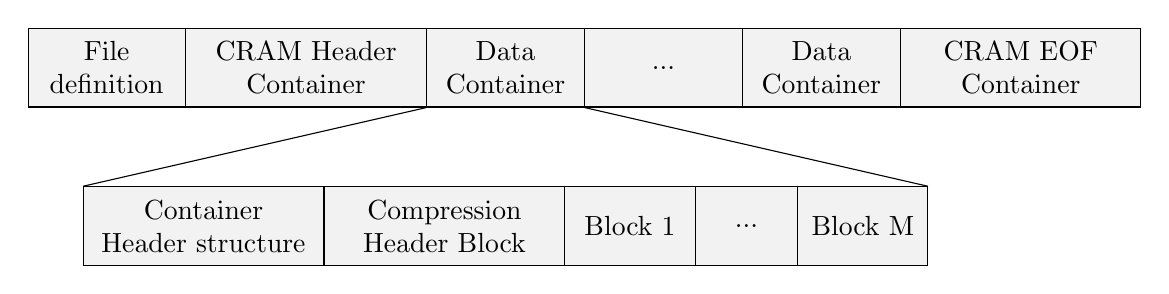
\begin{tikzpicture}[
  every node/.style={scale=1.0},
  boxes/.style={rectangle split,rectangle split parts=#1,draw,rectangle split horizontal,text width=5em,align=center,minimum height=1cm,fill=black!5,on grid},
  notes/.style={text width=20em,align=center,minimum height=1cm,on grid},
]
\node (file) [boxes=6] {
\nodepart{one}File definition
\nodepart[text width=8em]{two}CRAM Header Container
\nodepart{three}Data Container
\nodepart{four}...
\nodepart{five}Data Container
\nodepart[text width=8em]{six}CRAM EOF Container
};

\node (container) [boxes=5,below=1 of file.three south,text width=8em] {
\nodepart{one}Container Header structure
\nodepart{two}Compression Header Block
\nodepart[text width=4em]{three}Block 1
\nodepart[text width=3em]{four}...
\nodepart[text width=4em]{five}Block M
};
\draw (file.two split south) to (container.north west);
\draw (file.three split south) to (container.north east);
\end{tikzpicture}

Figure 3: Containers as a series of blocks
\end{center}

The Data Containers hold the sequence records themselves.
These start with a Compression Header block which holds meta-data
describing how and where the Data Series are encoded within this
container.

\begin{center}
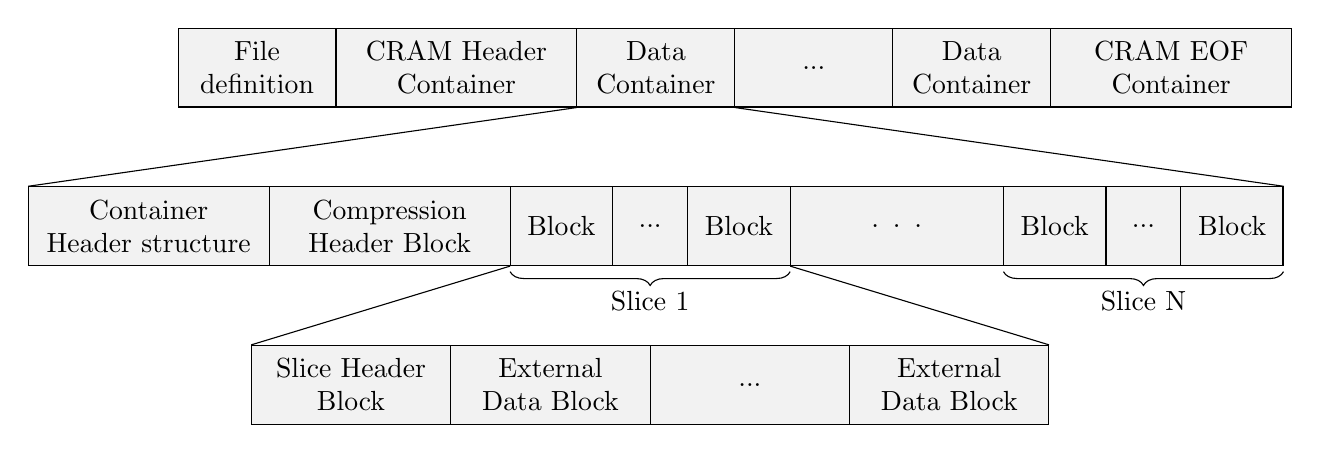
\begin{tikzpicture}[
  every node/.style={scale=1.0},
  boxes/.style={rectangle split,rectangle split parts=#1,draw,rectangle split horizontal,text width=5em,align=center,minimum height=1cm,fill=black!5,on grid},
  notes/.style={text width=20em,align=center,minimum height=1cm,on grid},
]
\node (file) [boxes=6] {
\nodepart{one}File definition
\nodepart[text width=8em]{two}CRAM Header Container
\nodepart{three}Data Container
\nodepart{four}...
\nodepart{five}Data Container
\nodepart[text width=8em]{six}CRAM EOF Container
};

\node (container) [boxes=9,below=1 of file.three south,text width=8em] {
\nodepart{one}Container Header structure
\nodepart{two}Compression Header Block
\nodepart[text width=3em]{three}Block
\nodepart[text width=2em]{four}...
\nodepart[text width=3em]{five}Block
\nodepart[text width=7em]{six}. . .
\nodepart[text width=3em]{seven}Block
\nodepart[text width=2em]{eight}...
\nodepart[text width=3em]{nine}Block
};
\draw (file.two split south) to (container.north west);
\draw (file.three split south) to (container.north east);

\draw[decoration={brace,mirror,amplitude=5pt,raise=2pt},decorate]
  (container.two split south) to (container.five split south);
\node [below=0.2 of container.four south] {Slice 1};

\draw[decoration={brace,mirror,amplitude=5pt,raise=2pt},decorate]
  (container.six split south) to (container.south east);
\node [below=0.2 of container.eight south] {Slice N};

\node (slice) [boxes=4,below=1 of container.four south, text width=6.5em] {
\nodepart{one}Slice Header Block
\nodepart{two}External Data Block
\nodepart{three}...
\nodepart{four}External Data Block
};
\draw (container.two split south) to (slice.north west);
\draw (container.five split south) to (slice.north east);
\end{tikzpicture}

Figure 4: Slices formed from a series of concatenated blocks
\end{center}

The blocks after the compression header are organised logically into slices. One 
slice may contain, for example, a contiguous region of alignment data. Slices begin 
with a slice header block and are followed by one or more data blocks.
It is these data blocks which hold the primary bulk of CRAM data, the
Data Series.

Note many CRAM files will just use one slice per contaner as this is
the default output format of several major implementations.

\subsection{File definition}

Each CRAM file starts with a fixed length (26 bytes) definition with the following 
fields:

\begin{tabular}{|l|l|l|}
\hline
\textbf{Data type} & \textbf{Name} & \textbf{Value}\tabularnewline
\hline
byte[4] & format magic number & CRAM (0x43 0x52 0x41 0x4d)\tabularnewline
\hline
byte & major format number & 3 (0x3)\tabularnewline
\hline
byte & minor format number & 1 (0x1)\tabularnewline
\hline
byte[20] & file id & CRAM file identifier (e.g. file name or SHA1 checksum)\tabularnewline
\hline
\end{tabular}

Valid CRAM \textit{major}.\textit{minor} version numbers are as follows:

\begin{itemize}
\item[\textit{1.0}]
The original public CRAM release.

\item[\textit{2.0}]
The first CRAM release implemented in both Java and C; tidied up
implementation vs specification differences in \textit{1.0}.

\item[\textit{2.1}]
Gained end of file markers; compatible with \textit{2.0}.

\item[\textit{3.0}]
Additional compression methods; header and data checksums;
improvements for unsorted data.

\item[\textit{3.1}]
Additional block compression codecs only.

\item[\textit{4.0}]
This specification.  Revised variable sized integers, MD/NM/RG tag
locators, and deduplication of read names.  Removed some encodings.
See \ref{sec:cram4changes} for a more detailed list of changes.
\end {itemize}

CRAM 3.0 and 3.1 differ only in the list of compression
methods available, so tools that output CRAM 3 without using any 3.1
codecs should write the header to indicate 3.0 in order to permit
maximum compatibility.

\subsection{Container header structure}

The file definition is followed by one or more containers with the following header 
structure where the container content is stored in the `blocks' field:

\begin{tabular}{|l|>{\raggedright}p{120pt}|>{\raggedright}p{260pt}|}
\hline
\textbf{Data type} & \textbf{Name} & \textbf{Value}
\tabularnewline
\hline
uint7 & length & the sum of the lengths of all blocks in this container (headers and data);
equal to the total byte length of the container minus the byte length of this header structure\tabularnewline
\hline
int7 & reference sequence id & reference sequence identifier  or\linebreak{}
-1 for unmapped reads\linebreak{}
-2 for multiple reference sequences.\linebreak{}
All slices in this container must have a reference sequence id matching this value.\tabularnewline
\hline
uint7 & starting position on the reference & the alignment start position or\linebreak{}
0 if the container is multiple-reference
or contains unmapped unplaced reads\tabularnewline
\hline
uint7 & alignment span & the length of the alignment or\linebreak{}
0 if the container is multiple-reference
or contains unmapped unplaced reads\tabularnewline
\hline
uint7 & number of records & number of records in the container\tabularnewline
\hline
uint7 & record counter & 1-based sequential index of records in the file/stream.\tabularnewline
\hline
uint7 & bases & number of read bases\tabularnewline
\hline
uint7 & number of blocks & the total number of blocks in this container\tabularnewline
\hline
array<uint7> & landmarks & the locations of slices in this container as byte offsets from the end of 
this container header, used for random access indexing.
The landmark count must equal the slice count.\linebreak{}
Since the block before the first slice is the compression header,
landmarks[0] is equal to the byte length of the compression header.\tabularnewline
\hline
uint32 & crc32 & CRC32 hash of the all the preceding bytes in the container.\tabularnewline
\hline
byte[ ] & blocks & The blocks contained within the container.\tabularnewline
\hline
\end{tabular}

\subsubsection*{CRC32}
This is a cyclic redundancy checksum 32-bit long with the polynomial 0x04C11DB7. Please refer to \href{http://www.itu.int/rec/recommendation.asp?type=folders&lang=e&parent=T-REC-V.42}{ITU-T V.42} for more details. The value of the CRC32 hash function is written as an integer.


\subsection{Block structure}
\label{sec:block-struct}

Containers consist of one or more blocks. Block compression is applied independently 
and in addition to any encodings used to compress data within the block. The block 
have the following header structure with the data stored in the `block data' field:

\begin{tabular}{|l|>{\raggedright}p{120pt}|>{\raggedright}p{260pt}|}
\hline
\textbf{Data type} & \textbf{Name} & \textbf{Value}
\tabularnewline
\hline
byte & method & the block compression method (and first CRAM version): \linebreak{}
0: raw (none)*\linebreak{}
1: gzip\linebreak{}
2: bzip2 (v2.0)\linebreak{}
3: lzma (v3.0)\linebreak{}
4: rans4x8 (v3.0)\linebreak{}
5: rans4x16 (v3.1)\linebreak{}
6: adaptive arithmetic coder (v3.1)\linebreak{}
7: fqzcomp (v3.1)\linebreak{}
8: name tokeniser (v3.1)
\tabularnewline
\hline
byte & block content type id & the block content type identifier\tabularnewline
\hline
uint7 & block content id & the block content identifier used to associate
data blocks with data series\tabularnewline
\hline
uint7 & size in bytes* & size of the block data after applying block compression\tabularnewline
\hline
uint7 & raw size in bytes* & size of the block data before applying block compression\tabularnewline
\hline
byte[ ] & block data & the data stored in the block\tabularnewline
\hline
uint32 & CRC32 & CRC32 hash value for all preceding bytes in the block\tabularnewline
\hline
\end{tabular}

* Note on raw method: both compressed and raw sizes must be set to the same value.

\subsubsection*{Block content types}
\label{subsec:block-content-types}

CRAM has the following block content types:

\begin{threeparttable}[t]
\begin{tabular}{|>{\raggedright}p{143pt}|>{\raggedright}p{45pt}|>{\raggedright}p{116pt}|>{\raggedright}p{114pt}|}
\hline
\textbf{Block content type} & \textbf{Block content type id} & \textbf{Name} & \textbf{Contents}\tabularnewline
\hline
FILE\_HEADER & 0 & CRAM header block & CRAM header\tabularnewline
\hline
COMPRESSION\_HEADER & 1 & Compression header block & See specific section\tabularnewline
\hline
SLICE\_HEADER & 2 & Slice header block & See specific section\tabularnewline
\hline
 & 3 &  & reserved\tabularnewline
\hline
EXTERNAL\_DATA & 4 & data block & data produced by encodings\tabularnewline
\hline
\end{tabular}
\end{threeparttable}

\subsubsection*{Block content id}

Block content id is used to distinguish between data blocks in the same slice. 
Each encoding has an id parameter which must be one of the block
content ids. For data blocks the content id is a positive integer. For all
other blocks content id should be 0. Consequently, all data encodings must 
not use content id less than 1. 

\subsection{CRAM header container}

The first container in a CRAM file contains a textual header in a single block, optionally
gzip compressed. This text header currently matches the SAM header specification. Only
gzip is allowed as compression method for this block. The CRAM header container does not
include a compression header block.

The following constraints apply to the SAM header: 

\begin{itemize}
\item The SQ:MD5 checksum is required unless the reference sequence has been embedded 
into the file.
\end{itemize}

It is recommended to reserve 50\% more space in the CRAM header container than
is required for the SAM header text by optionally padding the container with a second
raw block consisting of all zeroes. This can be used to subsequently expand the header
container in place, such as when updating @SQ records, while preserving the absolute
offsets of all subsequent containers.

\subsection{Compression header block}
\label{subsec:compression-header}

The compression header block consists of 3 parts: preservation map, data series 
encoding map and tag encoding map.  See below for the data format of a map.

These are meta-data on what is stored in the following slices, how it is encoded, and in which blocks the raw byte streams from these encodings reside.

\begin{tabular}{|l|>{\raggedright}p{120pt}|>{\raggedright}p{260pt}|}
\hline
\textbf{Data type} & \textbf{Name} & \textbf{Value}
\tabularnewline
\hline
map & preservation map & meta-data about types of data stored and dictionaries \tabularnewline
\hline
map & data series encoding map & meta-data for how data series are encoded \tabularnewline
\hline
map & tag encoding map & meta-data for how tags are encoded \tabularnewline
\hline
\end{tabular}

\subsubsection{Map structure}

% FIXME: is this better defined as a sub-structure in the relevant section itself?
% Possibly...
A \textit{Map} is a collection of keys and associated values.

Both the size in bytes and the number of keys are written as integer (uint7). Keys 
and values are written according to their data types and are specific to each map.
Keys have a fixed size for all items in a map, but this size is not
the same for all map types.  The order of keys is not defined.  Values
are stored immediately after their key in a key-defined format.  Some
keys will have simple boolean values, some are fixed size, while
others have a more complex sub-structures.

The example below is for a two byte key map.

\begin{tabular}{|l|>{\raggedright}p{120pt}|>{\raggedright}p{260pt}|}
\hline
\textbf{Data type} & \textbf{Name} & \textbf{Value}
\tabularnewline
\hline
uint7 & size & the remaining size in bytes of this map structure\tabularnewline
\hline
uint7 & num\_keys & the number of key-value pairs in this map\tabularnewline
\hline
byte[2] & key & first key\tabularnewline
\hline
byte[] & value & first value, with a key-specific size (see below).\tabularnewline
\hline
... & ... & \textit{repeated num\_keys time}\tabularnewline
\hline
\end{tabular}


\subsubsection{Preservation map}

The preservation map contains information about which data was preserved in the 
CRAM file. It is stored as a map with byte[2] keys:

\begin{tabular}{|l|l|>{\raggedright}p{100pt}|>{\raggedright}p{220pt}|}
\hline
\textbf{Key} & \textbf{Value data type} & \textbf{Name} & \textbf{Value}\tabularnewline
\hline
RN & bool & read names included & true if read names are preserved for all reads\tabularnewline
\hline
AP & bool & AP data series delta & true if AP data series is delta, false otherwise\tabularnewline
\hline
RR & bool & reference required & true if reference sequence is required to restore 
the data completely\tabularnewline
\hline
SM & byte[5] & substitution matrix & substitution matrix\tabularnewline
\hline
TD & array\texttt{<}byte\texttt{<>} & tag ids dictionary & a list of lists of tag ids, see tag encoding 
section\tabularnewline
\hline
QO & bool & qual orientation & true if quality values are in the same orientation as sequence.  If false quality values are recorded in the orientation as produced by the sequencing instrument, which may also still match sequence orientation.\tabularnewline
\hline
\end{tabular}

The boolean values are optional, defaulting to true when absent, although it is recommended to explicitly set them.  SM and TD are mandatory.

\subsubsection{Encoding structure}

The data series encoding map utilises another custom data type, \textit{encoding\texttt{<}type\texttt{>}}.
This is used to describe the data encapsulation format for a specific data series; how and where the values are stored.  This could be
the definition of a constant, a series of data transformations, or the
block content id for a data block.  Some encodings may be nested,
such as \texttt{BYTE\_ARRAY\_LEN} which defines one sub-encoding for the
length and another for the bytes.

Encoding notation is defined as the keyword `encoding' followed by its data type in angular brackets, for example `encoding\texttt{<}byte\texttt{>}' stands for an encoding that operates on a data series of data type `byte'.
Note there are distinct encodings dealing with signed and unsigned
data in addition to offsets applies to each, so for integer data the
data series use `encoding\texttt{<}int\texttt{>}` and let the specific
encoding and meta-data handle the sign as appropriate.

The \textit{encoding} format consists of an encoding type and type specific meta-data stored as an array (dimension followed by the array elements).

\begin{tabular}{|l|>{\raggedright}p{120pt}|>{\raggedright}p{260pt}|}
\hline
\textbf{Data type} & \textbf{Name} & \textbf{Value}
\tabularnewline
\hline
uint7 & encoding\_ID & encoding type identifier\tabularnewline
\hline
array\texttt{<}byte\texttt{>} & encoding\_meta & type specific meta-data for this encoding, serialised as a byte stream\tabularnewline
\hline
\end{tabular}

\vskip 10pt

Note unlike the fields in structures, data series types here do not
distinguish signed integer (sint) vs unsigned integer (uint) as this
distinction is handled by the encoding itself.  This is different to
CRAM 3.0 and earlier where the sign and size of the data series types
was written into the specification, rather than stored as meta-data in
the CRAM file.

For example, the alignment position (\textbf{AP}) data series has a value data type of \textit{encoding<int>}.
Typically on a position sorted file this is delta encoded and all
values are positive, so a suitable encoding is VARINT\_UNSIGNED.  If
the slice contains data aligned against multiple reference sequences
then this may contain some negative deltas in which case
VARINT\_SIGNED could be appropriate.

A list of data types along with their possible encodings is listed
below.

\begin{tabular}{llll}
\textbf{ID}  & \textbf{Encoding} & \textbf{Data Type} & \textbf{Description}\\
\hline
\\
0  & NULL             & \textit{N/A} & Data series not present\\
\\
1  & BYTE (EXTERNAL)  & byte   & An unsigned single byte (8 bits)  \\
\\
4  & BYTE\_ARRAY\_LEN & byte[] & Zero or more items with unspecified length\\
5  & BYTE\_ARRAY\_STOP& byte[] & Zero or more items with unspecified length\\
\\
41 & VARINT\_UNSIGNED & int    & A variable length integer (VLQ $x >= 0$)\\
42 & VARINT\_SIGNED   & int    & A variable length integer (VLQ, may be negative)\\
\\
43 & CONST\_BYTE      & byte   & A fixed byte value\\
44 & CONST\_INT       & int    & A fixed integer value (VLQ, signed)\\
\end{tabular}

\vskip 10pt

See section~\ref{sec:encodings} for more detailed descriptions of all
the above coding algorithms and their parameters.  Note the encoding
ID values here have been chosen to not clash with CRAM 3.0 and earlier
with the exception of the BYTE\_ARRAY\_LEN and BYTE\_ARRAY\_STOP
encodings which have not changed and BYTE which is identical and
synonymous with EXTERNAL in the CRAM 3.0 specification.

\subsubsection{Data series encoding map}

Writing to and reading from data blocks is organised through CRAM
records. A CRAM record is analogous to a single line in a SAM file.

The records are organised into slices and then each slice is
rearranged in a columnar fashion into data series.  For example
collect 10,000 SAM records and then the first column, query name
(QNAME), becomes one CRAM data series (RN), the next column (FLAG)
becomes CRAM data series (BF), and so on.  Note some SAM columns, such
as CIGAR, may map to many CRAM data series.

Each data series is associated with an encoding. An encoding may have
a block content id which is used to identify the block where the data
series is stored. Please note that data blocks can have multiple
data series associated with them; in this case the values from these
data series will be interleaved and must be decoded in the correct order.

\begin{center}
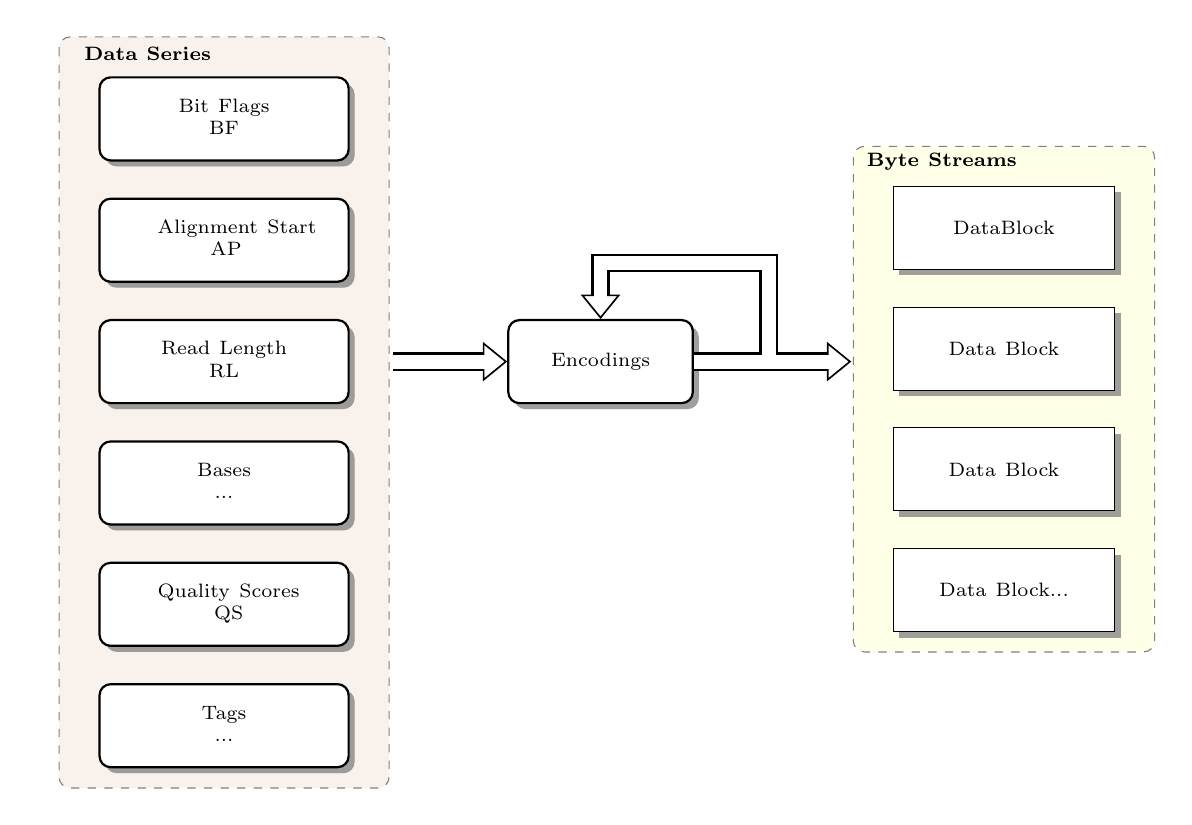
\begin{tikzpicture}[thick]

\usetikzlibrary{shapes, shadows, positioning, arrows,  decorations.markings, arrows.meta}

\pgfdeclarelayer{background}
\pgfsetlayers{background,main}

\tikzstyle{dsbox} = [blockbox, text width=6em, minimum width=9em, minimum height=3em, rounded corners, drop shadow]
\tikzstyle{blockbox}=[draw, fill=white, text width=4.0em, text centered, minimum height=1.0em, drop shadow]
\tikzstyle{encodedblock} = [blockbox, text width=6em, minimum width=8em, minimum height=3em, drop shadow]
\tikzstyle{encodings} = [dsbox, minimum width=6em, thick]

\tikzstyle{texto} = [above, text width=8em, text centered]

\tikzstyle{vecArrow} = [thick, decoration={markings,mark=at position
   1 with {\arrow[semithick]{Triangle[open, length=3.1mm, width=5mm]}}},
   double distance=5pt, shorten >= 8.5pt,
   preaction = {decorate},
   postaction = {draw,line width=5pt, white,shorten >= 8pt}]
\tikzstyle{innerWhite} = [semithick, white,line width=5pt, shorten >= 8pt]

\newcommand{\cramRecord}[6]{%
\begin{pgfonlayer}{background}
    \path (#1.west |- #1.north) + (-0.5, 0.5) node (a1) {};
    \path (#1.east |- #6.south) + (+0.5,-0.25) node (a2) {};
    \path[fill=brown!10,rounded corners, draw=black!50, dashed]
      (a1) rectangle (a2);
    \path (a1.east |- a1.south) + (1.0,-0.3) node[texto]
    {\scriptsize\textbf{Data Series}};
\end{pgfonlayer}}

\newcommand{\dsbox}[2]{node (p#1) [dsbox]
{\scriptsize{#2}}}
\newcommand{\encodedblock}[2]{node (p#1) [encodedblock]
	{\scriptsize{#2}}}
\newcommand{\encodedblocklarge}[2]{node (p#1) [encodedblocklarge]
   {\scriptsize{#2}}}

\path +(-2.5,-1.5) \dsbox{1}{\begin{tabular}{c} Bit Flags \\ BF \end{tabular}};
\path (p1.south)+(0.0,-1.0) \dsbox{2}{\begin{tabular}{c} Alignment Start\\ AP\quad\quad \end{tabular}};
\path (p2.south)+(0.0,-1.0) \dsbox{3}{\begin{tabular}{c} Read Length \\ RL \end{tabular}};
\path (p3.south)+(0.0,-1.0) \dsbox{4}{\begin{tabular}{c} Bases \\ ... \end{tabular}};
\path (p4.south)+(0.0,-1.0) \dsbox{5}{\begin{tabular}{c} Quality Scores \\ QS \end{tabular}};
\path (p5.south)+(0.0,-1.0) \dsbox{6}{\begin{tabular}{c} Tags \\ ... \end{tabular}};

\cramRecord{p1}{p2}{p3}{p4}{p5}{p6}

\newcommand{\blockStreams}[4]{%
\begin{pgfonlayer}{background}
    \path (#1.west |- #1.north)+(-0.5, 0.5) node (a3) {};
    \path (#4.east |- #4.south)+(+0.5, -0.25) node (a4) {};
    \path[fill=yellow!10, rounded corners, draw=black!50, dashed]
      (a3) rectangle (a4);
    \path (a3.east |- a3.south)+(1.0,-0.3) node[texto]{\scriptsize\textbf{Byte Streams}};
\end{pgfonlayer}}

\path (a1.south) + (12.0, -2.3) \encodedblock {7} {DataBlock};
\path (p7.south) + (0.0, -1.0)  \encodedblock {8} {Data Block};
\path (p8.south) + (0.0, -1.0)  \encodedblock {9} {Data Block}; 
\path (p9.south) + (0.0, -1.0)  \encodedblock {10}{Data Block...};

\blockStreams {p7} {p8} {p9} {p10}

\node (encodings) [encodings, right = 2 of p3] {\scriptsize Encodings};
\node (enc_e1) [right=0.7 of encodings] {};
\node (enc_e2) [right=1.05 of enc_e1] {};
\node (enc_n)  [above=1 of encodings.center] {};
\draw[vecArrow] (p3.east) + (0.55, 0) to (encodings.west);
\draw[vecArrow] (encodings.east) to (enc_e2.west);
\draw[vecArrow] (enc_e1.east) |- (enc_n.north) to (encodings.north);
\draw[innerWhite] (encodings.east) to (enc_e2.west);

\end{tikzpicture}

Figure 5: The relationship between Data Series, Possibly nested Encodings, and Data Blocks.

\end{center}

The picture shows how a CRAM record (on the left) is distributed to
multiple Data Blocks via a series of encodings.  Note the mapping from
Data Series to Blocks may be many to many, with the possibility of
multiple Data Series writing to the same Block and with a single
encoding such as BYTE\_ARRAY\_LEN potentially writing to two Blocks.


Each data series has an encoding. These encodings are stored in a map with byte[2] 
keys and are decoded in approximately this order\footnote{The precise order is defined in section~\ref{sec:record}.}:

\begin{threeparttable}[t]
\begin{tabular}{|l|l|>{\raggedright}p{100pt}|>{\raggedright}p{220pt}|}
\hline
\textbf{Key} & \textbf{Value data type} & \textbf{Name} & \textbf{Value}\tabularnewline
\hline
BF & encoding\texttt{<}int\texttt{>} & BAM bit flags & see separate section\tabularnewline
\hline
CF & encoding\texttt{<}int\texttt{>} & CRAM bit flags & see specific section\tabularnewline
\hline
RI & encoding\texttt{<}int\texttt{>} & reference id & record reference id from
the SAM file header\tabularnewline
\hline
RL & encoding\texttt{<}int\texttt{>} & read lengths & read lengths\tabularnewline
\hline
AP & encoding\texttt{<}int\texttt{>} & in-seq positions & if \textbf{AP-Delta} = true: 0-based alignment start
delta from the AP value in the previous record.
Note this delta may be negative, for example when switching references in a multi-reference slice.
When the record is the first in the slice, the previous position used is the slice alignment-start field (hence the first delta should be zero for single-reference slices, or the AP value itself for multi-reference slices).  \linebreak{}
if \textbf{AP-Delta} = false: encodes the alignment start position directly\tabularnewline
\hline
RG & encoding\texttt{<}int\texttt{>} & read groups & read groups. Special value 
`-1' stands for no group.\tabularnewline
\hline
RN\tnote{a} & encoding\texttt{<}byte[ ]\texttt{>} & read names & read names\tabularnewline
\hline
MF & encoding\texttt{<}int\texttt{>} & next mate bit flags & see specific section\tabularnewline
\hline
NS & encoding\texttt{<}int\texttt{>} & next fragment reference sequence id & reference 
sequence ids for the next fragment \tabularnewline
\hline
NP & encoding\texttt{<}int\texttt{>} & next mate alignment start & alignment positions 
for the next fragment\tabularnewline
\hline
TS & encoding\texttt{<}int\texttt{>} & template size & template sizes\tabularnewline
\hline
NF & encoding\texttt{<}int\texttt{>} & distance to next fragment & number of records
to the next fragment\tnote{b}\tabularnewline
\hline
TL\tnote{c} & encoding\texttt{<}int\texttt{>} & tag ids  & list of tag ids, see tag encoding
section\tabularnewline
\hline
FN & encoding\texttt{<}int\texttt{>} & number of read features & number of read
features in each record\tabularnewline
\hline
FC & encoding\texttt{<}byte\texttt{>} & read features codes & see separate section\tabularnewline
\hline
FP & encoding\texttt{<}int\texttt{>} & in-read positions & positions of the read
features; a positive delta to the last position (starting with zero)\tabularnewline
\hline
DL & encoding\texttt{<}int\texttt{>} & deletion lengths & base-pair deletion lengths\tabularnewline
\hline
BB & encoding\texttt{<}byte[ ]\texttt{>} & stretches of bases & bases\tabularnewline
\hline
QQ & encoding\texttt{<}byte[ ]\texttt{>} & stretches of quality scores & quality scores\tabularnewline
\hline
BS & encoding\texttt{<}byte\texttt{>} & base substitution codes & base substitution
codes\tabularnewline
\hline
IN & encoding\texttt{<}byte[ ]\texttt{>} & insertion & inserted bases\tabularnewline
\hline
RS & encoding\texttt{<}int\texttt{>} & reference skip length & number of skipped 
bases for the `N' read feature\tabularnewline
\hline
PD & encoding\texttt{<}int\texttt{>} & padding & number of padded bases\tabularnewline
\hline
HC & encoding\texttt{<}int\texttt{>} & hard clip & number of hard clipped bases\tabularnewline
\hline
SC & encoding\texttt{<}byte[ ]\texttt{>} & soft clip & soft clipped bases\tabularnewline
\hline
MQ & encoding\texttt{<}int\texttt{>} & mapping qualities & mapping quality scores\tabularnewline
\hline
BA & encoding\texttt{<}byte\texttt{>} & bases & bases\tabularnewline
\hline
QS & encoding\texttt{<}byte\texttt{>} & quality scores & quality scores\tabularnewline
\hline
\end{tabular}

\begin{tablenotes}
\item[a] Note RN this is decoded after MF if the record is detached from the mate and we are attempting to auto-generate read names.
\item[b] The count is reset for each slice so NF can only refer to a record later within this slice.
\item[c] Decode of TL is followed by decoding the tag values themselves, in order of appearance in the tag dictionary.
\end{tablenotes}
\end{threeparttable}

\subsubsection{Tag encoding map}
\label{subsubsec:tags}

The tag dictionary (TD) describes the unique combinations of tag id / type that occur on each alignment record.
For example if we search the id / types present in each record and find only two combinations -- X1:i BC:Z SA:Z: and X1:i: BC:Z -- then we have two dictionary entries in the TD map.

Let $L_{i}=\{T_{i0}, T_{i1}, \ldots, T_{ix}\}$ be a list of all tag ids for a record $R_{i}$, where $i$ is the sequential record index and $T_{ij}$ denotes $j$-th tag id in the record.
The list of unique $L_{i}$ is stored as the TD value in the preservation map.
Maintaining the order is not a requirement for encoders (hence ``combinations''), but it is permissible and thus different permutations, each encoded with their own elements in TD, should be supported by the decoder.
Each $L_{i}$ element in TD is assigned a sequential integer number starting with 0.
These integer numbers are referred to by the TL data series.
Using TD, an integer from the TL data series can be mapped back into a list of tag ids.
Thus per alignment record we only need to store tag values and not their ids and types.

The TD is written as a byte array consisting of $L_{i}$ values separated with \textbackslash{}0.
Each $L_{i}$ value is written as a concatenation of 3 byte $T_{ij}$ elements: tag id followed by BAM tag type code (one of A, c, C, s, S, i, I, f, F, Z, H or B, as described in the SAM specification) or \texttt{*}.
Type code \texttt{*} is used as a placeholder to mark the presence and location of the MD, NM or RG tags.

For example the TD for tag lists X1:i BC:Z SA:Z and X1:i MD:Z NM:i BC:Z may be encoded as\\
X1CBCZSAZ\textbackslash{}0X1CMD*NM*BCZ\textbackslash{}0, with X1C indicating a 1 byte unsigned value for tag X1 and an assumption that all MD and NM tags present can be auto-generated.

\subsubsection*{Tag values}

The encodings used for different tags are stored in a map.
The key is 3 bytes formed from the BAM tag id and type code, matching the TD dictionary described above.
Unlike the Data Series Encoding Map, the key is stored in the map as a uint7 encoded integer, constructed using $(char1<<16) + (char2<<8) + type$.
For example, the 3-byte representation of OQ:Z is \{0x4F, 0x51, 0x5A\} and these bytes are intepreted as the integer key 0x004F515A, leading to an uint7 byte stream \{0x82, 0xbd, 0xa2, 0x59\}.

\begin{tabular}{|l|l|l|>{\raggedright}p{160pt}|}
\hline
\textbf{Key} & \textbf{Value data type} & \textbf{Name} & \textbf{Value}
\tabularnewline
\hline
TAG ID 1:TAG TYPE 1 & encoding\texttt{<}byte[ ]\texttt{>} & read tag 1 & tag values
(names and types are available in the data series code)\tabularnewline
\hline
... &  & ... & ...\tabularnewline
\hline
TAG ID N:TAG TYPE N & encoding\texttt{<}byte[ ]\texttt{>} & read tag N & ...\tabularnewline
\hline
\end{tabular}

Note that tag values are encoded as array of bytes. The routines to convert tag 
values into byte array and back are the same as in BAM with the exception of value 
type being captured in the tag key rather in the value.
Hence consuming 1 byte for types `C' and `c', 2 bytes for types `S' and `s', 4 bytes for types `I', `i' and `f', and a variable number of bytes for types `H', `Z' and `B'.

\subsection{Slice header block}

The slice header block is never compressed (block method=raw). For reference mapped 
reads the slice header also defines the reference sequence context of the data 
blocks associated with the slice. Mapped reads can be stored along with
\textbf{placed unmapped}\footnote{Unmapped reads can be \textit{placed} or \textit{unplaced}.
A read that is unmapped according to bit 0x4 of the BF (BAM bit flags)
data series, but has position and reference fields filled in, is
\textit{placed unmapped}.  In contrast, \textit{unplaced unmapped}
reads have have a reference sequence ID of -1 and alignment position of 0.}
reads on the same reference within the same slice.

Slices with the Multiple Reference flag (-2) set as the sequence ID in the header may contain reads
mapped to multiple external references, including unmapped\footnotemark[\value{footnote}] reads (placed on these references or unplaced),
but multiple embedded references cannot be combined in this way.  When multiple references are
used, the RI data series will be used to determine the reference sequence ID for each record.  This
data series is not present when only a single reference is used within a slice.

The Unmapped (-1) sequence ID in the header is for slices containing only unplaced
unmapped\footnotemark[\value{footnote}] reads.

A slice containing data that does not use the external reference in
any sequence may set the reference MD5 sum to zero.  This can happen
because the data is unmapped or the sequence has been stored verbatim
instead of via reference-differencing.  This latter scenario is
recommended for unsorted or non-coordinate-sorted data.

The slice header block contains the following fields.

\begin{tabular}{|l|l|>{\raggedright}p{200pt}|}
\hline
\textbf{Data type} & \textbf{Name} & \textbf{Value}\tabularnewline
\hline
int7 & reference sequence id & reference sequence identifier or\linebreak{}
-1 for unmapped reads\linebreak{}
-2 for multiple reference sequences.\linebreak{}
This value must match that of its enclosing container.\tabularnewline
\hline
uint7 & alignment start & the alignment start position.\linebreak{}
0 if the slice is multiple-reference
or contains unmapped unplaced reads\tabularnewline
\hline
uint7 & alignment span & the length of the alignment.\linebreak{}
0 if the slice is multiple-reference
or contains unmapped unplaced reads\tabularnewline
\hline
uint7 & number of records & the number of records in the slice\tabularnewline
\hline
uint7 & record counter & 1-based sequential index of records in the file/stream\tabularnewline
\hline
uint7 & number of blocks & the number of blocks in the slice\tabularnewline
\hline
uint7[ ] & block content ids & block content ids of the blocks in the slice\tabularnewline
\hline
uint7 & embedded reference bases block content id & block content id for the embedded 
reference sequence bases or 0 for none\tabularnewline
\hline
byte[16] & reference md5 & MD5 checksum of the reference bases within the slice 
boundaries.  If this slice has reference sequence id of -1 (unmapped) or -2 (multi-ref)
the MD5 should be 16 bytes of \textbackslash{}0. For embedded references, the MD5
can either be all-zeros or the MD5 of the embedded sequence.\tabularnewline
\hline
byte[] & optional tags & a series of tag,type,value tuples encoded as
per BAM auxiliary fields.\tabularnewline
\hline
\end{tabular}

The optional tags are encoded in the same manner as BAM tags.  I.e. a
series of binary encoded tags concatenated together where each tag
consists of a 2 byte key (matching [A-Za-z][A-Za-z0-9]) followed by a
1 byte type ([AfZHcCsSiIB]) followed by a string of bytes in a format
defined by the type.

Tags starting in a capital letter are reserved while lowercase ones or
those starting with X, Y or Z are user definable.  Any tag not
understood by a decoder should be skipped over without producing an
error.

At present no tags are defined, but potential uses include additional
checksums and statistical information.

% Details omitted until we fully work through all the corner cases,
% such as seq/qual of *.
%
% Reserved tags are defined as follows:
% 
% \begin{tabular}{|l|l|>{\raggedright}p{325pt}|}
% \hline
% \textbf{Tag type} & \textbf{BAM format} & \textbf{Meaning}\tabularnewline
% \hline
% BD & i & Sum over all reads of the CRC32 hash of sequence base.  This
% may be used to validate round-trips in and out of CRAM.
% calls\tabularnewline
% \hline
% SD & i & Sum over all reads of the CRC32 hash of quality scores. (If
% the quality string is ``*'' in SAM then the hash is of the BAM encoded
% version - a string of bytes with value 255.)\tabularnewline
% \hline
% \end{tabular}


\subsection{End of file container}

A special container is used to mark the end of a file or stream. It is required in version 3 or later.
The idea is to provide an easy and a quick way to detect that a CRAM file or stream is complete.
The marker is an empty container with ref seq id set to -1 (unaligned) and alignment start set to 4542278 (which is ``EOF'' when seen in ASCII).

It is recommended that implementations of CRAM validate EOF by checking these values rather than direct comparison of byte values, as these checks will be valid for all versions of CRAM

\section{Record structure}
\label{sec:record}

CRAM record is based on the SAM record but has additional features allowing for 
more efficient data storage.  In contrast to BAM record CRAM records
are separated by type of data into a series of data blocks.  These
blocks can then use content type aware compression techniques.

As CRAM data series may be interleaved within the same blocks\footnote{Interleaving can sometimes provide better compression, however it also adds dependency between types of data meaning it is not possible to selectively decode one data series if it co-locates with another data series in the same block.} understanding the order in which CRAM data series must be decoded is vital.

The overall flowchart is below, with more detailed description in the subsequent sections.

\algnewcommand\algorithmicto{\text{ \textbf{to} }}

\subsection{CRAM record}

Both mapped and unmapped reads start with the following fields. Please note that 
the data series type refers to the logical data type and the data series name corresponds 
to the data series encoding map.

\begin{tabular}{|>{\raggedright}p{70pt}|>{\raggedright}p{75pt}|>{\raggedright}p{90pt}|>{\raggedright}p{171pt}|}
\hline
\textbf{Data series type} & \textbf{Data series name} & \textbf{Field} & \textbf{Description}\tabularnewline
\hline
uint & BF & BAM bit flags & see BAM bit flags below\tabularnewline
\hline
uint & CF & CRAM bit flags & see CRAM bit flags below\tabularnewline
\hline
- & - & Positional data & See section \ref{subsec:positions}\tabularnewline
\hline
- & - & Read names & See section \ref{subsec:names}\tabularnewline
\hline
- & - & Mate records & See section \ref{subsec:mate}\tabularnewline
\hline
- & - & Auxiliary tags & See section \ref{subsec:tags}\tabularnewline
\hline
- & - & Sequences & See sections \ref{subsec:mapped} and \ref{subsec:unmapped}\tabularnewline
\hline
\end{tabular}

\subsubsection*{BAM bit flags (BF data series)}

The following flags are duplicated from the SAM and BAM specification, with identical meaning.
Note however some of these flags can be derived during decode, so may be omitted in the CRAM file and the bits computed based on both reads of a pair-end library residing within the same slice.

\begin{threeparttable}[t]
\begin{tabular}{|l|l|l|}
\hline
\textbf{Bit flag} & \textbf{Comment} & \textbf{Description}\tabularnewline
\hline
0x1 &  & template having multiple segments in sequencing\tabularnewline
\hline
0x2 &  & each segment properly aligned according to the aligner\tabularnewline
\hline
0x4 &  & segment unmapped\tnote{a}\tabularnewline
\hline
0x8 & calculated\tnote{b}\ \ or stored in the mate's info & next segment in template unmapped\tabularnewline
\hline
0x10 &  & SEQ being reverse complemented\tabularnewline
\hline
0x20 & calculated\tnote{b}\ \ or stored in the mate's info & SEQ of the next segment in the
template being reverse complemented\tabularnewline
\hline
0x40 &  & the first segment in the template\tnote{c}\tabularnewline
\hline
0x80 &  & the last segment in the template\tnote{c}\tabularnewline
\hline
0x100 &  & secondary alignment\tabularnewline
\hline
0x200 &  & not passing quality controls\tabularnewline
\hline
0x400 &  & PCT or optical duplicate\tabularnewline
\hline
0x800 &  & Supplementary alignment\tabularnewline
\hline
\end{tabular}
\begin{tablenotes}
\item[a] Bit 0x4 is the only reliable place to tell whether the read is unmapped.  If 0x4 is set, no assumptions may be made about bits 0x2, 0x100 and 0x800.
\item[b] For segments within the same slice.
\item[c] Bits 0x40 and 0x80 reflect the read ordering within each template inherent in the sequencing technology used, which may be independent from the actual mapping orientation.
If 0x40 and 0x80 are both set, the read is part of a linear template (one where the template sequence is expected to be in a linear order), but it is neither the first nor the last read.
If both 0x40 and 0x80 are unset, the index of the read in the template is unknown.
This may happen for a non-linear template (such as one constructed by stitching together other templates) or when this information is lost during data processing.
\end{tablenotes}
\end{threeparttable}

\subsubsection*{CRAM bit flags (CF data series)}

The CRAM bit flags (also known as compression bit flags) expressed as an integer represent the CF data series. 
The following compression flags are defined for each CRAM read record:

\begin{tabular}{|>{\raggedright}p{39pt}|>{\raggedright}p{150pt}|>{\raggedright}p{242pt}|}
\hline
\textbf{Bit flag} & \textbf{Name} & \textbf{Description}\tabularnewline
\hline
0x1 & quality scores stored as array & quality scores can be stored as read features
or as an array similar to read bases.\tabularnewline
\hline
0x2 & detached & mate information is stored verbatim (e.g. because the pair spans multiple slices or the fields differ to the CRAM computed method)\tabularnewline
\hline
0x4 & has mate downstream & tells if the next segment should be expected further
in the stream\tabularnewline
\hline
0x8 & decode sequence as ``*'' & informs the decoder that the sequence
is unknown and that any encoded reference differences are present only to
recreate the CIGAR string.\tabularnewline
\hline
0x10 & explicit template size & decode from the template size (TS) data series even for record in an attached pair.\tabularnewline
\hline
\end{tabular}


The following pseudocode describes the general process of decoding an entire CRAM record.
The sequence data itself is in one of two encoding formats depending on whether the record is aligned (mapped).

\subsubsection*{Decode pseudocode}
\newlength{\maxwidth}
\newcommand{\algalign}[2] % #1 = text to left, #2 = text to right
{\makebox[\maxwidth][l]{$#1{}$}${}#2$}

\begin{algorithmic}[1]
\Procedure{DecodeRecord}{}
\settowidth{\maxwidth}{CRAM\_flags\quad}
\State \algalign{BAM\_flags}{\gets}  \Call{ReadItem}{BF, Integer}
\State \algalign{CRAM\_flags}{\gets} \Call{ReadItem}{CF, Integer}
\State \Call{DecodePositions}{}\Comment{See section \ref{subsec:positions}}
\State \Call{DecodeNames}{}\Comment{See section \ref{subsec:names}}
\State \Call{DecodeMateData}{}\Comment{See section \ref{subsec:mate}}
\State \Call{DecodeTagData}{}\Comment{See section \ref{subsec:tags}}
\Statex

\If{$(BF$ AND $4) \ne 0$}\Comment{Unmapped flag}
  \State \Call{DecodeMappedRead}{}\Comment{See section \ref{subsec:mapped}}
\Else
  \State \Call{DecodeUnmappedRead}{}\Comment{See section \ref{subsec:unmapped}}
\EndIf
\EndProcedure
\end{algorithmic}

\subsection{CRAM positional data}
\label{subsec:positions}

Following the bit-wise BAM and CRAM flags, CRAM encodes positional related data including reference, alignment positions and length, and read-group.
Positional data is stored for both mapped and unmapped sequences, as unmapped data may still be ``placed'' at a specific location in the genome (without being aligned).
Typically this is done to keep a sequence pair (paired-end or mate-pair sequencing libraries) together when one of the pair aligns and the other does not.

For reads stored in a position-sorted slice, the AP-delta flag in the compression header preservation map should be set and the AP data series will be delta encoded, using the slice alignment-start value as the first position to delta against.
Note for multi-reference slices this may mean that the AP series includes negative values, such as when moving from an alignment to the end of one reference sequence to the start of the next or to unmapped unplaced data.  When the AP-delta flag is not set the AP data series is stored as a normal integer value.

\begin{tabular}{|>{\raggedright}p{70pt}|>{\raggedright}p{75pt}|>{\raggedright}p{90pt}|>{\raggedright}p{171pt}|}
\hline
\textbf{Data series type} & \textbf{Data series name} & \textbf{Field} & \textbf{Description}\tabularnewline
\hline
int & RI & ref id & reference sequence id (only present in multiref slices)\tabularnewline
\hline
int & RL & read length & the length of the read\tabularnewline
\hline
int & AP & alignment start & the alignment start position\tabularnewline
\hline
int & RG & read group & the read group identifier expressed as the N\textsuperscript{th} record in the header, starting from 0 with -1 for no group\tabularnewline
\hline
\end{tabular}

\vskip 20pt
\begin{algorithmic}[1]
\Procedure{DecodePositions}{}
\If{$slice\_header.reference\_sequence\_id = -2$}
  \State $reference\_id\gets$ \Call{ReadItem}{RI, Integer}
\Else
  \State $reference\_id\gets slice\_header.reference\_sequence\_id$
\EndIf
\State $read\_length \gets$ \Call{ReadItem}{RL, Integer}
\If{$container\_pmap.AP\_delta \ne 0$}
    \If{$first\_record\_in\_slice$}
        \State $last\_position\gets$ $slice\_header.alignment\_start$
    \EndIf
    \State $alignment\_position \gets$ \Call{ReadItem}{AP, Integer} + $last\_position$
    \State $last\_position \gets alignment\_position$
\Else
    \State $alignment\_position \gets$ \Call{ReadItem}{AP, Integer}
\EndIf
\State $read\_group \gets$ \Call{ReadItem}{RG, Integer}
\EndProcedure
\end{algorithmic}

\subsection{Read names (RN data series)}
\label{subsec:names}

Read names can be preserved in the CRAM format, but this is optional and is governed by the \texttt{RN} preservation map key in the container compression header. See section \ref{subsec:compression-header}.
When read names are not preserved the CRAM decoder should generate names, typically based on the file name and a numeric ID of the read using the record counter field of the slice header block.
Note read names may still be preserved even when the \texttt{RN} compression header key indicates otherwise, such as where a read is part of a read-pair and the pair spans multiple slices.
In this situation the record will be marked as detached (see the CF data series) and the mate data below (section \ref{subsec:mate}) will contain the read name.

\begin{tabular}{|>{\raggedright}p{70pt}|>{\raggedright}p{75pt}|>{\raggedright}p{90pt}|>{\raggedright}p{171pt}|}
\hline
\textbf{Data series type} & \textbf{Data series name} & \textbf{Field} & \textbf{Description}\tabularnewline
\hline
byte[] & RN & read names & read names\tabularnewline
\hline
\end{tabular}

\vskip 20pt
\begin{algorithmic}[1]
\Procedure{DecodeNames}{}
\State $read\_name \gets empty$
\If{$container\_pmap.read\_names\_included = 1$}
  \State $read\_name \gets$ \Call{ReadItem}{RN, Byte[]}
\EndIf
\Statex
\EndProcedure
\end{algorithmic}

\subsection{Mate record}
\label{subsec:mate}

There are two ways in which mate information can be preserved in CRAM: number of records downstream (distance, within this slice) to the next fragment in the template and a special mate record if the next fragment is not in the current slice.
In the latter case the record is labelled as ``detached'', see the CF data series.

For mates within the slice only the distance is captured, and only for the first record.  The mate has neither detached nor downstream flags set in the CF data series.

\begin{tabular}{|>{\raggedright}p{68pt}|>{\raggedright}p{115pt}|>{\raggedright}p{228pt}|}
\hline
\textbf{Data series type} & \textbf{Data series name} & \textbf{Description}\tabularnewline
\hline
int & NF & the number of records to the next fragment\tabularnewline
\hline
\end{tabular}

In the above case, the NS (mate reference name), NP (mate position) and TS (template size) fields for both records should be derived once the mate has also been decoded.
Mate reference name and position are obvious and simply copied from the mate.
The template size is computed using the method described in the SAM specification; the inclusive distance from the leftmost to rightmost mapped bases with the sign being positive for the leftmost record and negative for the rightmost record.

If the next fragment is not found within this slice then the following structure is included into the CRAM record.
Note there are cases where read-pairs within the same slice may be marked as detached and use this structure, such as to store mate-pair information that does not match the algorithm used by CRAM for computing the mate data on-the-fly.

\begin{tabular}{|>{\raggedright}p{66pt}|>{\raggedright}p{117pt}|>{\raggedright}p{228pt}|}
\hline
\textbf{Data series type} & \textbf{Data series name} & \textbf{Description}\tabularnewline
\hline
int & MF & next mate bit flags, see table below\tabularnewline
\hline
byte[ ] & RN & the read name (if and only if not known already)\tabularnewline
\hline
int & NS & mate reference sequence identifier \tabularnewline
\hline
int & NP & mate alignment start position \tabularnewline
\hline
int & TS & the size of the template (insert size)\tabularnewline
\hline
\end{tabular}

\subsubsection*{Next mate bit flags (MF data series)}

The next mate bit flags expressed as an integer represent the MF data series.
These represent the missing bits we excluded from the BF data series (when compared to the full SAM/BAM flags).
The following bit flags are defined:

\begin{tabular}{|>{\raggedright}p{47pt}|>{\raggedright}p{134pt}|>{\raggedright}p{250pt}|}
\hline
\textbf{Bit flag} & \textbf{Name} & \textbf{Description}\tabularnewline
\hline
0x1 & mate negative strand bit & the bit is set if the mate is on the negative
strand\tabularnewline
\hline
0x2 & mate unmapped bit & the bit is set if the mate is unmapped\tabularnewline
\hline
\end{tabular}


\subsubsection*{Decode mate pseudocode}

\begin{algorithmic}[1]
\Procedure{DecodeMateData}{}
\If{$CF\bitand 2$}\Comment{Detached from mate}
  \State $mate\_flags\gets $ \Call{ReadItem}{MF,Integer}
  \If{$mate\_flags\bitand 1$}
    \State $bam\_flags\gets bam\_flags\bitor$ 0x20\Comment{Mate is reverse-complemented}
  \EndIf
  \If{$mate\_flags\bitand 2$}
    \State $bam\_flags\gets bam\_flags\bitor$ 0x08\Comment{Mate is unmapped}
  \EndIf
  \If{$container\_pmap.read\_names\_included \ne 1$}
    \State $read\_name \gets$ \Call{ReadItem}{RN, Byte[]}
  \EndIf
\settowidth{\maxwidth}{mate\_position\ }
\State \algalign{mate\_ref\_id}{\gets}  \Call{ReadItem}{NS, Integer}
\State \algalign{mate\_position}{\gets} \Call{ReadItem}{NP, Integer}
\State \algalign{template\_size}{\gets} \Call{ReadItem}{TS, Integer}
\ElsIf{$CF\bitand 16$}\Comment{Explicit template size}
  \State $template\_size\gets$ \Call{ReadItem}{TS, Integer}
\EndIf
\EndProcedure
\end{algorithmic}

Note as with the SAM specification a template may be permitted to have more than two alignment records.
In this case the ``mate'' for each record is considered to be the next record, with the mate for the last record being the first to form a circular list.
The above algorithm is a simplification that does not deal with this scenario.
The full method needs to observe when record $this+NF$ is also labelled as having an additional mate downstream.
One recommended approach is to resolve the mate information in a second pass, once the entire slice has been decoded.
The final segment in the mate chain needs to set $bam\_flags$ fields 0x20 and 0x08 accordingly based on the first segment.
This is also not listed in the above algorithm, for brevity.

\subsection{Auxiliary tags}
\label{subsec:tags}

Tags are encoded using a tag line (TL data series) integer into the tag dictionary (TD field in the compression header preservation map, see section \ref{subsec:compression-header}).
See section \ref{subsubsec:tags} for a more detailed description of this process.

\begin{tabular}{|>{\raggedright}p{70pt}|>{\raggedright}p{75pt}|>{\raggedright}p{90pt}|>{\raggedright}p{200pt}|}
\hline
\textbf{Data series type} & \textbf{Data series name} & \textbf{Field} & \textbf{Description}\tabularnewline
\hline
int & TL & tag line & an index into the tag dictionary (TD)\tabularnewline
\hline
\textit{various} & \textit{various} & tag name/type & 3 character key (2 tag identifier and 1 tag type), as specified by the tag dictionary\tabularnewline
\hline
\end{tabular}

\vskip 20pt
\begin{algorithmic}[1]
\Procedure{DecodeTagData}{}
\State $tag\_line\gets$ \Call{ReadItem}{TL,Integer}
\ForAll {$ele \in container\_pmap.tag\_dict(tag\_line)$}
  \State $name\gets$ first two characters of $ele$
  \State $tag(type)\gets$ last character of $ele$
  \If{$tag(type) = ``*''$}
  \State $tag(name)\gets$ \Call{GenerateTag}{$name$}
  \Else
  \State $tag(name)\gets$ \Call{ReadItem}{$ele$, Byte[]}\Comment{Type specific}
  \EndIf
\EndFor
\EndProcedure
\end{algorithmic}

In the above procedure, $name$ is a two letter tag name and $type$ is one of the permitted types documented in the SAM/BAM specification.
Type is \texttt{c} (signed 8-bit integer), \texttt{C} (unsigned 8-bit integer), \texttt{s} (signed 16-bit integer), \texttt{S} (unsigned 16-bit integer), \texttt{i} (signed 32-bit integer), \texttt{I} (unsigned 32-bit integer), \texttt{f} (32-bit float), \texttt{Z} (nul-terminated string), \texttt{H} (nul-terminated string of hex digits) and \texttt{B} (binary data in array format with the first byte being one of c,C,s,S,i,I,f using the meaning above, a 32-bit integer for the number of array elements, followed by array data encoded using the specified format).  All integers are little endian encoded.

For example a SAM tag \texttt{MQ:i} has name \texttt{MQ} and type \texttt{i} and will be decoded using one of MQc, MQC, MQs, MQS, MQi and MQI data series depending on size and sign of the integer value.

Note some auxiliary tags can be created automatically during decode so can optionally be removed by the encoder.
However if the decoder finds a tag stored verbatim it should use this in preference to automatically computing the value.

The RG (read group) auxiliary tag should be created if the read group (RG data series) value is not $-1$.

The MD and NM auxiliary tags store the differences (an edit string) between the sequence and the reference along with the number of mismatches.
These may optionally be created on-the-fly during reference-based sequence reconstruction and should match the description provided in the SAMtags document.
An encoder may decide to store these verbatim when no reference is used or where the automatically constructed values differ to the input data.

The tag type \texttt{*} is used in conjunction with MD, NM and RG as a flag to indicate that this tag is present but is not being stored verbatim.
(If MD is being stored verbatim, we would expect MDZ in the TD dictionary for this tag line.)
The \texttt{*} type is also useful for ensuring the ordering of tags can be preserved.

Note it is permitted for decoders to choose to auto-generate MD and NM tags even in the absence of MD* and NM* entries.

\subsection{Mapped reads}
\label{subsec:mapped}

\subsubsection*{Read feature records}
\label{subsec:features}

Read features are used to store read details that are expressed using read coordinates 
(e.g. base differences respective to the reference sequence). The read feature 
records start with the number of read features followed by the read features themselves.
Each read feature has the position encoded as the distance since the
last feature position, or the absolute position (i.e. delta vs zero)
for the first feature.
Finally the single mapping quality and per-base quality scores are stored.

\begin{threeparttable}[t]
\begin{tabular}{|>{\raggedright}p{88pt}|>{\raggedright}p{83pt}|>{\raggedright}p{85pt}|>{\raggedright}p{180pt}|}
\hline
\textbf{Data series type} & \textbf{Data series name} & \textbf{Field} & \textbf{Description}\tabularnewline
\hline
int & FN & number of read features & the number of read features\tabularnewline
\hline
int & FP & in-read-position\tnote{a} & position of the read feature\tabularnewline 
\hline
byte & FC & read feature code\tnote{a} & See feature codes below\tabularnewline
\hline
* & * & read feature data\tnote{a} & See feature codes below\tabularnewline
\hline
int & MQ & mapping qualities & mapping quality score\tabularnewline
\hline
byte[read length] & QS & quality scores & the base qualities, if preserved\tabularnewline
\hline
\end{tabular}
\begin{tablenotes}
\item[a] Repeated FN times, once for each read feature.
\end{tablenotes}
\end{threeparttable}

\subsubsection*{Read feature codes}

Each feature code has its own associated data series containing further information specific to that feature.
The following codes are used to distinguish variations in read coordinates:

\begin{tabular}{|>{\raggedright}p{91pt}|>{\raggedright}p{45pt}|>{\raggedright}p{72pt}|>{\raggedright}p{66pt}|>{\raggedright}p{132pt}|}
\hline
\textbf{Feature code} & \textbf{Id} & \textbf{Data series type} & \textbf{Data 
series name} & \textbf{Description}\tabularnewline
\hline
Bases & b (0x62) & byte[ ] & BB & a stretch of bases\tabularnewline
\hline
Scores & q (0x71) & byte[ ] & QQ & a stretch of scores\tabularnewline
\hline
% Neither C nor Java implementations generator nor can decode the 'A'
% feature code, but if they did they'd be BB/QQ and not BA/QS.  Best
% to omit it from published spec for now?
%
% Bases and scores & A (0x41) & byte[ ],byte[ ] & BB,QQ & A a stretch of bases and
% quality scores score\tabularnewline
% \hline
Read base & B (0x42) & byte,byte & BA,QS & A base and associated quality score\tabularnewline
\hline
Substitution & X (0x58) & byte & BS & base substitution codes, SAM operators X, 
M and =\tabularnewline
\hline
Insertion & I (0x49) & byte[ ] & IN & inserted bases, SAM operator I\tabularnewline
\hline
Deletion & D (0x44) & int & DL & number of deleted bases, SAM operator D\tabularnewline
\hline
Insert base & i (0x69) & byte & BA & single inserted base, SAM operator I\tabularnewline
\hline
Quality score & Q (0x51) & byte & QS & single quality score\tabularnewline
\hline
Reference skip & N (0x4E) & int & RS & number of skipped bases, SAM operator N\tabularnewline
\hline
Soft clip & S (0x53) & byte[ ] & SC & soft clipped bases, SAM operator S\tabularnewline
\hline
Padding & P (0x50) & int & PD & number of padded bases, SAM operator P\tabularnewline
\hline
Hard clip & H (0x48) & int & HC & number of hard clipped bases, SAM operator H\tabularnewline
\hline
\end{tabular}

\subsubsection*{Base substitution codes (BS data series)}

A base substitution is defined as a change from one nucleotide base (reference base) to
another (read base), including N as an unknown or missing base. There are 5 possible reference
bases (ACGTN), with 4 possible substitutions for each base, and 20 substitutions in total.
The codes for all possible substitutions are stored in a substitution matrix. To restore a
base, one would use the reference base and the substitution code, resolving the base via lookup
in the substitution matrix.

\subsubsection*{Substitution Matrix Format}

Each of the 4 possible substitutions for a given reference base is assigned a 2-bit integer
code (see below) with a value ranging from 0 to 3 inclusive. The 4 2-bit codes are packed
into a single byte, high 2-bits first, for each base ACGTN (minus the reference base itself).
The entire substitution matrix is written as 5 such bytes, one for each reference base, also
in the order ACGTN.

\subsubsection*{Substitution Code Assignment}

To assign the susbtitution code for a given reference base/read base, the substitutions for
each reference base may optionally be sorted by their frequencies, in descending order, with
same-frequency ties broken using the fixed order ACGTN. Although sorting by substitution
frequency is not required by the CRAM format, assigning substitution codes based on frequency
maximizes compression by ensuring that the most frequent substitutions use the shortest possible
codes.

For example, let us assume the following substitution frequencies for base A: 

AC: 15\%

AG: 25\%

AT: 55\%

AN: 5\%

Then the substitution codes are: 

AC: 2

AG: 1

AT: 0

AN: 3

The first byte of the substitution matrix entry for reference base A is written as a single byte,
with the codes in the order CGTN: 10 01 00 11 = 147 decimal, or 0x93 in this case. This will then
be followed by 4 more bytes representing substitutions for reference bases C, G, T and N.

\subsubsection*{Decode mapped read pseudocode}

\begin{algorithmic}[1]
\Procedure{DecodeMappedRead}{}
  \State $feature\_number\gets$ \Call{ReadItem}{FN, Integer} 
  \State $last\_feature\_position\gets 0$
  \For{$i\gets 1 \algorithmicto feature\_number$}
    \State \Call{DecodeFeature}{}
  \EndFor
  \State $mapping\_quality\gets$ \Call{ReadItem}{MQ, Integer} 
  \If{$container\_pmap.preserve\_quality\_scores$}
    \If{$(container\_pmap.qual\_orientation = 0) \logand (bam\_flags \bitand 0x10)$}
      \For{$i\gets 0 \algorithmicto read\_length-1$}
        \State $quality\_score_{read\_length-1-i}\gets$ \Call{ReadItem}{QS, Integer} 
       \EndFor
    \Else
      \For{$i\gets 0 \algorithmicto read\_length-1$}
        \State $quality\_score_i\gets$ \Call{ReadItem}{QS, Integer} 
       \EndFor
    \EndIf
  \EndIf
\EndProcedure
\Statex
\Procedure{DecodeFeature}{}
    \settowidth{\maxwidth}{feature\_position\ }
    \State \algalign{feature\_code}{\gets}       \Call{ReadItem}{FC, Integer} 
    \State \algalign{feature\_position}{\gets}   \Call{ReadItem}{FP, Integer} $+\ last\_feature\_position$
    \State $last\_feature\_position\gets feature\_position$
    \settowidth{\maxwidth}{substitution\_code\ }
    \If{$feature\_code = $`B'}
      \State \algalign{base}{\gets}              \Call{ReadItem}{BA, Byte}
      \State \algalign{quality\_score}{\gets}    \Call{ReadItem}{QS, Byte}
    \ElsIf{$feature\_code = $`X'}
      \State \algalign{substitution\_code}{\gets} \Call{ReadItem}{BS, Byte}
    \ElsIf{$feature\_code = $`I'}
      \State \algalign{inserted\_bases}{\gets}   \Call{ReadItem}{IN, Byte[]}
    \ElsIf{$feature\_code = $`S'}
      \State \algalign{softclip\_bases}{\gets}   \Call{ReadItem}{SC, Byte[]}
    \ElsIf{$feature\_code = $`H'}
      \State \algalign{hardclip\_length}{\gets}  \Call{ReadItem}{HC, Integer}
    \ElsIf{$feature\_code = $`P'}
      \State \algalign{pad\_length}{\gets}       \Call{ReadItem}{PD, Integer}
    \ElsIf{$feature\_code = $`D'}
      \State \algalign{deletion\_length}{\gets}  \Call{ReadItem}{DL, Integer}
    \ElsIf{$feature\_code = $`N'}
      \State \algalign{ref\_skip\_length}{\gets} \Call{ReadItem}{RS, Integer}
    \ElsIf{$feature\_code = $`i'}
      \State \algalign{base}{\gets}              \Call{ReadItem}{BA, Byte}
    \ElsIf{$feature\_code = $`b'}
      \State \algalign{bases}{\gets}             \Call{ReadItem}{BB, Byte[]}
    \ElsIf{$feature\_code = $`q'}
      \State \algalign{quality\_scores}{\gets}   \Call{ReadItem}{QQ, Byte[]}
    \ElsIf{$feature\_code = $`Q'}
      \State \algalign{quality\_score}{\gets}    \Call{ReadItem}{QS, Byte}
    \EndIf
\EndProcedure
\end{algorithmic}

\subsection{Unmapped reads}
\label{subsec:unmapped}

The CRAM record structure for unmapped reads has the following additional fields:

\begin{tabular}{|>{\raggedright}p{88pt}|>{\raggedright}p{83pt}|>{\raggedright}p{85pt}|>{\raggedright}p{180pt}|}
\hline
\textbf{Data series type} & \textbf{Data series name} & \textbf{Field} & \textbf{Description}\tabularnewline
\hline
byte[read length] & BA & bases & the read bases\tabularnewline
\hline
byte[read length] & QS & quality scores & the base qualities, if preserved\tabularnewline
\hline
\end{tabular}

\vskip20pt
\begin{algorithmic}[1]
\Procedure{DecodeUnmappedRead}{}
  \For{$i\gets 1 \algorithmicto read\_length$}
    \State $base\gets$ \Call{ReadItem}{BA, Byte}
  \EndFor
  \If{$container\_pmap.preserve\_quality\_scores$}
    \If{$(container\_pmap.qual\_orientation = 0) \logand (bam\_flags \bitand 0x10)$}
      \For{$i\gets 0 \algorithmicto read\_length-1$}
        \State $quality\_score_{read\_length-1-i}\gets$ \Call{ReadItem}{QS, Integer} 
       \EndFor
    \Else
      \For{$i\gets 0 \algorithmicto read\_length-1$}
        \State $quality\_score_i\gets$ \Call{ReadItem}{QS, Integer} 
       \EndFor
    \EndIf
  \EndIf
\EndProcedure
\end{algorithmic}

\subsection{Resolving inter-record dependencies}

Some entries in a record can only be filled out after decoding
the entire slice, such as the computed PNEXT, RNEXT and TLEN SAM
fields and reversing the deduplication of read names (QNAME).

Thus \textsc{DecodeRecord} is considered as part of a wider \textsc{DecodeSlice} procedure.
This procedure is rather complicated so best understood with the addition of pseudocode.

If a record has read the next fragment (NF) data series, then it is has some data that has been deduplicated (not stored verbatim for each record in the template) and is expected to be computed.
All such records will have mate position updated and some BAM flags (mate unmapped, mate reverse) set, as well as setting the paired in sequencing flag.

If such a record also has an undefined template size, meaning the TS data series has not yet been read, this is derived by finding the leftmost and rightmost alignment records and provided they all map to the same reference the template size (SAM TLEN field) is set.  Normally the leftmost read has a positive TLEN value, but special care is made for cases where multiple records are mapped to the leftmost position in which case the record with BAM flag READ1 is defined to be the positive one.

Finally read names (SAM QNAME field) may have been deduplicated too.
If a record has an empty name and also has the next fragment defined, the record name is copied from this next fragment

If the read name is still empty, the name is auto-generated.  It is suggested that this is based on the global record count in the file and some predefined prefix.

\begin{algorithmic}[1]
\Procedure{DecodeSlice}{}
\State \Call{DecodeSliceHeader}{}
\For{$i\gets 0 \algorithmicto num\_recs-1$}
  \State \Call{DecodeRecord}{$rec_i$}
\EndFor
% FIXME: should this be from num_recs-1 to 0 so next_frag works
% with 3+ fragments, with last being actual copy?
\For{$i\gets 0 \algorithmicto num\_recs-1$}
  \If{$rec_i.next\_frag \ne undefined$}
    \State \Call{ResolvePair}{$i$}
  \EndIf
  \State \Call{ResolveName}{$i$}
\EndFor
\EndProcedure
\end{algorithmic}

\begin{algorithmic}[1]
\Procedure{ResolvePair}{$rnum$}
  \State $i \gets rnum$
  \If{$rec_i.template\_size = undefined$}
    \State $(leftmost,\ rightmost,\ same\_ref) \gets$ \Call{FindLeftRight}{$i$}

    \If{$same\_ref = 1$} \Comment{Template entirely mapped to one reference sequence}
      \State $j \gets i$
      \Repeat
        \If{$rec_j.position = leftmost$}
          \If{$left\_count = 1 \logor rec_j.bam\_flags \bitand$ 0x40}
            \State $rec_j.template\_size \gets tlen$\Comment{Use READ1 flag as tie-breaker if same location}
          \Else
            \State $rec_j.template\_size \gets -tlen$
          \EndIf
        \Else
          \State $rec_j.template\_size \gets -tlen$
        \EndIf
        \State $j \gets j + 1 + rec_j.next\_ref$
      \Until{$j = i$}
    \Else \Comment{Template spans multiple references}
      \State $j \gets i$
      \Repeat
        \State $rec_j.template\_size \gets 0$
        \State $j \gets j + 1 + rec_j.next\_ref$
      \Until{$j = i$}
    \EndIf
  \EndIf

  \Statex\Comment{Ensure other pairing data is complete}
  \State $j \gets j + 1 + rec_i.next\_ref$
  \State $rec_i.mate\_position \gets rec_j.mate\_position$
  \State $rec_i.bam\_flags \gets rec_i.bam\_flags \bitor 1$ \Comment{Set BAM PAIRED flag}
  \If{$rec_j.bam\_flags \bitand 16$}\Comment{BAM REVERSE flag}
    \State $rec_i.bam\_flags \gets rec_i.bam\_flags \bitor 32$
  \EndIf
  \If{$rec_j.bam\_flags \bitand 4$}\Comment{BAM UNMAPPED flag}
    \State $rec_i.bam\_flags \gets rec_i.bam\_flags \bitor 8$
  \EndIf
  \State 
\EndProcedure
\end{algorithmic}

\begin{algorithmic}[1]
\Function{FindLeftRight}{$rnum$}
  \State $i \gets rnum$
  \State $leftmost \gets rec_i.position$\Comment{Find leftmost and rightmost record}
  \State $rightmost \gets rec_i.end\_position$\Comment{Computed from POS + CIGAR}
  \State $same\_ref \gets 1$
  \State $left\_count \gets 0$\Comment{Count of number of records at leftmost pos}
  \State $j \gets i$
  \Repeat
    \If{$leftmost > ref_j.position$}
      \State $leftmost \gets ref_j.position$
      \State $left\_count \gets 1$
    \ElsIf{$leftmost = ref_j.position$}
      \State $left\_count \gets left\_count + 1$
    \EndIf
    \If{$rightmost < ref_j.end\_position$}
      \State $rightmost \gets ref_j.end\_position$
    \EndIf
    \If{$rec_i.ref \ne rec_j.ref$}
      \State $same\_ref \gets 0$
    \EndIf
    \If{$rec_j.next\_frag \ne undefined$}
      \State $j \gets j + 1 + rec_j.next\_frag$
    \Else
      \State $j \gets i$
    \EndIf
  \Until{$j = i$}
  \Return $(leftmost,\ rightmost, \ same\_ref)$
\EndFunction
\end{algorithmic}

\begin{algorithmic}[1]
\Procedure{ResolveName}{rnum}
  \State $i \gets rnum$
  \If{$rec_i.read\_name = empty$}
    \If{$rec_i.cram\_flag \bitand 4$}
       \State $j \gets i + 1 + rec_i.next\_frag$
       \State $rec_i.read\_name = rec_j.read\_name$
    \EndIf
  \EndIf
  \If{$rec_i.name = empty$}
    \State $rec_i.read\_name \gets$ \Call{GenerateName}{}
  \EndIf
\EndProcedure
\end{algorithmic}

\section{Reference sequences}

CRAM format is natively based upon usage of reference sequences even though in 
some cases they are not required. In contrast to BAM format CRAM format has strict 
rules about reference sequences. 

\begin{enumerate}
\item M5 (sequence MD5 checksum) field of @SQ sequence record in the BAM header is 
required and UR (URI for the sequence fasta optionally gzipped file) field is strongly 
advised. The rule for calculating MD5 is to remove any non-base symbols (like \textbackslash{}n, 
sequence name or length and spaces) and upper case the rest. Here are some examples: 

\texttt{> samtools faidx human\_g1k\_v37.fasta 1 \textbar{} grep -v '\textasciicircum{}>' \textbar{} tr -d '\textbackslash{}n' \textbar{} tr a-z A-Z \textbar{} md5sum -\\
1b22b98cdeb4a9304cb5d48026a85128  -}

\texttt{> samtools faidx human\_g1k\_v37.fasta 1:10-20 \textbar{}grep -v '\textasciicircum{}\texttt{>}' \textbar{}tr -d '\textbackslash{}n' \textbar{}tr a-z A-Z \textbar{}md5sum -\\
0f2a4865e3952676ffad2c3671f14057  -}

Please note that the latter calculates the checksum for 11 bases from position 
10 (inclusive) to 20 (inclusive) and the bases are counted 1-based, so the first 
base position is 1. 

\item All CRAM reader implementations are expected to check for reference MD5 checksums 
and report any missing or mismatching entries. Consequently, all writer implementations 
are expected to ensure that all checksums are injected or checked during compression 
time. 

\item In some cases reads may be mapped beyond the reference sequence. All out of 
range reference bases are all assumed to be `N'. 

\item MD5 checksum bytes in slice header should be ignored for unmapped or multiref 
slices. 
\end{enumerate}

\section{Indexing}

\subsubsection*{General notes}

Indexing is only valid on coordinate (reference ID and then leftmost position) sorted files.

Please note that CRAM indexing is external to the file format itself and may change 
independently of the file format specification in the future. For example, a new 
type of index file may appear.

Individual records are not indexed in CRAM files, slices should be used instead 
as a unit of random access. Another important difference between CRAM and BAM indexing 
is that CRAM container header and compression header block (first block in container) 
must always be read before decoding a slice. Therefore two read operations are 
required for random access in CRAM.

Indexing a CRAM file is deemed to be a lightweight operation because it usually does not require any CRAM records to be read.
Indexing information can be obtained from container headers, namely sequence id, alignment start and span, container start byte offset and slice byte offset inside the container (landmarks).
The exception to this is with multi-reference containers, where the ``RI'' data series must be read.

\subsubsection*{CRAM index}

A CRAM index is a gzipped tab delimited file containing the following columns:

\begin{enumerate}
\item Reference sequence id

\item Alignment start (ignored on read for unmapped slices, set to 0 on write)

\item Alignment span (ignored on read for unmapped slices, set to 0 on write)

\item Absolute byte offset of Container header in the file.

\item Relative byte offset of the Slice header block, from the end of
the container header.  This is the same as the ``landmark'' field
in the container header.

\item Slice size in bytes (including slice header and all blocks).
\end{enumerate}

Each line represents a slice in the CRAM file.
Please note that all slices must be listed in the index file.

Multi-reference slices may need to have multiple lines for the same slice; one for each reference contained within that slice.
In this case the index reference sequence ID will be the actual reference ID (from the ``RI'' data series) and not -2.

Slices containing solely unmapped unplaced data (reference ID -1) still require values for all columns, although the alignment start and span will be ignored.
It is recommended that they are both set to zero.

To illustrate this the absolute and relative offsets used in a three slice container are shown in the diagram below.

\begin{center}
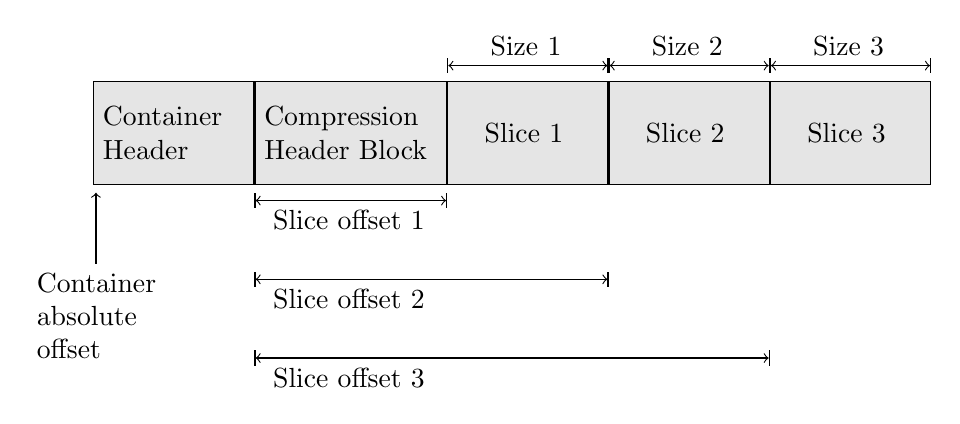
\begin{tikzpicture}[
  boxed/.style={rectangle, draw=black, fill=black!10, minimum height=1.3cm, text width=1.8cm},
]
\node(A) [boxed]{Container Header};
\node(B) [boxed,right,text width=2.2cm] at (A.east){Compression Header Block};
\node(C) [boxed,right] at (B.east){\quad Slice 1};
\node(D) [boxed,right] at (C.east){\quad Slice 2};
\node(E) [boxed,right] at (D.east){\quad Slice 3};

\draw[<-] (A.south west)+(1pt,-0.1cm) -- +(1pt,-1cm)
     node[below, text width=1.5cm]{Container absolute offset};


\draw[|<->|] ([yshift=-0.2cm]B.south west) node[below,xshift=1.2cm]{Slice offset 1}
    -- ([yshift=-0.2cm]B.south east);
\draw[|<->|] ([yshift=-1.2cm]B.south west) node[below,xshift=1.2cm]{Slice offset 2}
    -- ([yshift=-1.2cm]C.south east);
\draw[|<->|] ([yshift=-2.2cm]B.south west) node[below,xshift=1.2cm]{Slice offset 3}
    -- ([yshift=-2.2cm]D.south east);

\draw[|<->|] ([yshift=+0.2cm]C.north west) node[above,xshift=1cm]{Size 1} -- ([yshift=+0.2cm]C.north east);
\draw[|<->|] ([yshift=+0.2cm]D.north west) node[above,xshift=1cm]{Size 2} -- ([yshift=+0.2cm]D.north east);
\draw[|<->|] ([yshift=+0.2cm]E.north west) node[above,xshift=1cm]{Size 3} -- ([yshift=+0.2cm]E.north east);


\end{tikzpicture}
\end{center}

\subsubsection*{BAM index}

BAM indexes are supported by using 4-byte integer pointers called landmarks that 
are stored in container header. BAM index pointer is a 64-bit value with 48 bits 
reserved for the BAM block start position and 16 bits reserved for the in-block 
offset. When used to index CRAM files, the first 48 bits are used to store the 
CRAM container start position and the last 16 bits are used to store the index 
of the landmark in the landmark array stored in  container header. The landmark 
index can be used to access the appropriate slice. 

The above indexing scheme treats CRAM slices as individual records in BAM file. 
This allows to apply BAM indexing to CRAM files, however it introduces some overhead 
in seeking specific alignment start because all preceding records in the slice 
must be read and discarded.

\section{Encodings}
\label{sec:encodings}

% FIXME: we have a mishash of coding, encoding and codec.  We should
% go through the entire document and be consistent.

\subsection{Introduction}

The basic idea for encodings is to efficiently represent byte and integer values.
This can be achieved in a number of ways that most frequently involve some knowledge 
about the nature of the values being encoded, for example, distribution statistics. 
The methods for choosing the best encoding and determining its parameters are very 
diverse and are not part of the CRAM format specification, which only describes 
how the information needed to decode the values should be stored.

\subsection{BYTE}

This encoding simply stores byte values verbatim to a block with a given ID.

\subsubsection*{Parameters}

CRAM format defines the following parameters for BYTE encoding: 

\begin{tabular}{|>{\raggedright}p{100pt}|>{\raggedright}p{100pt}|>{\raggedright}p{230pt}|}
\hline
\textbf{Data type} & \textbf{Name} & \textbf{Comment}
\tabularnewline
\hline
uint7 & id & id of a block containing the byte stream\tabularnewline
\hline
\end{tabular}

\subsection{VARINT\_UNSIGNED}

This encoding stores unsigned integer values using the Variable Length Quantity
format (VLQ)\footnote{https://en.wikipedia.org/wiki/Variable-length\_quantity}.

It is not permitted to store any negative values using this encoding.
However given several data series have ranges that have the
possibility of small negative values (such as -1 for Alignment
Position), it is possible to skew the values slightly by adding an
offset prior to encoding.  This provides a mechanism for guaranteeing
all values remain positive.

Note this offset is added to the value after that value has been
decoded so to encode -1 we may wish to set offset to -1 and encode a
zero.  This mechanism may also be used to skew a range of values that
do not cluster around zero.  For example if a data series has values
ranging from 1000 to 1200, then setting offset to 1000 and encoding
values between 0 and 200 would provide a smaller data footprint.

For data series that require a broader scope of signed values we would
recommend using VARINT\_SIGNED instead.

\subsubsection*{Parameters}

CRAM format defines the following parameters for VARINT\_UNSIGNED encoding: 

\begin{tabular}{|>{\raggedright}p{100pt}|>{\raggedright}p{100pt}|>{\raggedright}p{230pt}|}
\hline
\textbf{Data type} & \textbf{Name} & \textbf{Comment}
\tabularnewline
\hline
sint7 & offset & amount to add to decoded values\tabularnewline
\hline
uint7 & id & id of a block containing the byte stream\tabularnewline
\hline
\end{tabular}

\subsection{VARINT\_SIGNED}

This encoding permits storing a broad range of both positive and
negative values while still following the property of low magnitude
values taking up less space than large magnitude ones.

It achieves this by using ZigZag encoding where signed values 0, -1,
+1, -2, +2 and so on are mapped to unsigned values 0, 1, 2, 3, 4.
These unsigned values are then stored using the same VLQ system used
by VARINT\_UNSIGNED.

As with VARINT\_UNSIGNED, an offset is added to the value after it has
been VLQ and ZigZag decoded.  Combined these permit efficient storage
of a distribution of values centred around a mean.  For example if
the distribution of values in a data series ranged from 1000 to 2000
with a peak at 1500, we could set offset to 1500 and encode values
-500 to +500.

\subsubsection*{Parameters}

CRAM format defines the following parameters for VARINT\_SIGNED encoding: 

\begin{tabular}{|>{\raggedright}p{100pt}|>{\raggedright}p{100pt}|>{\raggedright}p{230pt}|}
\hline
\textbf{Data type} & \textbf{Name} & \textbf{Comment}
\tabularnewline
\hline
sint7 & offset & amount to add to decoded values\tabularnewline
\hline
uint7 & id & id of a block containing the byte stream\tabularnewline
\hline
\end{tabular}


\subsection{CONST\_BYTE}

Sometimes a data series has a constant value throughout the
container.  In this case we can record this value in the Container
Compression Header and avoid the need to store the data series.

\subsubsection*{Parameters}

CRAM format defines the following parameters for CONST\_BYTE encoding: 

\begin{tabular}{|>{\raggedright}p{100pt}|>{\raggedright}p{100pt}|>{\raggedright}p{230pt}|}
\hline
\textbf{Data type} & \textbf{Name} & \textbf{Comment}
\tabularnewline
\hline
byte & value & the constant value\tabularnewline
\hline
\end{tabular}

\subsection{CONST\_INT}

As per CONST\_BYTE, but the value is a signed integer encoded with
VLQ and ZigZag methods.
The overhead of using ZigZag encoding on a constant unsigned value is
an average of 1 bit per container per use of this encoding.

\subsubsection*{Parameters}

CRAM format defines the following parameters for CONST\_INT encoding: 

\begin{tabular}{|>{\raggedright}p{100pt}|>{\raggedright}p{100pt}|>{\raggedright}p{230pt}|}
\hline
\textbf{Data type} & \textbf{Name} & \textbf{Comment}
\tabularnewline
\hline
sint & value & the constant value\tabularnewline
\hline
\end{tabular}

\subsection{BYTE\_ARRAY\_LEN (ID 4)}

Can encode types \textit{Byte[]}.

Often there is a need to encode an array of bytes where the length is
not predetermined.  For example the read identifiers differ per
alignment record, possibly with different lengths, and this length
must be stored somewhere.   Note in contrast to this, quality values
are known to be the same length as the sequence which is an already
known quantity, so the CRAM record encodes this using an implicit
array by asking for multiple values to be decoded rather than using an
explicit byte array encoding.

With BYTE\_ARRAY\_LEN the length is explicitly encoded via its own
sub-encoding prior to the array of bytes itself, also via its own
sub-encoding.

Note these sub-encodings may store the data in the same block, in
which case the length comes first. Alternatively we may decide that
the lengths have their own unique distribution which differs
substantially to the data itself and so should be stored in a
different block to permit better compression.  Having decoded the
length, the decoder must then call the value sub-encoding that many
times to retrieve the bytes.

Given the recursion used here of an encoding using two sub-encodings,
the byte stream for BYTE\_ARRAY\_LEN is the concatenation of both
sub-encodings.

\subsubsection*{Parameters}

The parameters for BYTE\_ARRAY\_LEN are listed below:

\begin{tabular}{|>{\raggedright}p{100pt}|>{\raggedright}p{100pt}|>{\raggedright}p{230pt}|}
\hline
\textbf{Data type} & \textbf{Name} & \textbf{Comment}
\tabularnewline
\hline
encoding\texttt{<}int\texttt{>} & lengths encoding & an encoding describing how 
the arrays lengths are stored\tabularnewline
\hline
encoding\texttt{<}byte\texttt{>} & values encoding & an encoding describing how 
the values (bytes) are stored\tabularnewline
\hline
\end{tabular}

\subsubsection*{Example}

The bytes for an X0:i SAM auxiliary field consisting of 16-bit items
may be written as an X0S tag line.  Despite the size being known, all
tag items are stored as byte arrays, so BYTE\_ARRAY\_LEN is ideal when
coupled with a CONST\_INT encoding to hold the fixed size lengths and
BYTE for the values.

\begin{tabular}{lll}
\hline
\textbf{Bytes} & & \textbf{Meaning}\\
\hline
\texttt{0x04}         & & BYTE\_ARRAY\_LEN encoding ID                                    \\
\texttt{0x07}         & & 7 remaining bytes of BYTE\_ARRAY\_LEN parameters            \\
\\
\texttt{0x44}         & & CONST\_INT encodng ID, for the aux tag lengths \\
\texttt{0x01}         & & remaining length of CONST\_INT encoding \\
\texttt{0x05}         & & length 2 as Zig-Zag format \\
\\
\texttt{0x01}         & & BYTE encoding ID, for the aux tag values \\
\texttt{0x02}         & & 2 more bytes of BYTE parameters                          \\
\texttt{0x81 0x48}    & & uint7 encoding for block ID 200                              \\
\hline
\end{tabular}

\subsection{BYTE\_ARRAY\_STOP (ID 5)}

Can encode types \textit{Byte[]}.

Instead of encoding an explicit length (as per BYTE\_ARRAY\_LEN) this
encoding stores bytes ending in a termination value.  The data
returned should not include this termination byte.  Hence this is
comparable to the C language string encoding, which uses a nul
character for termination, while BYTE\_ARRAY\_LEN is more similar to
the Pascal language string encoding.

Given this encoding is capturing the length within the same data
stream as the bytes, unlike BYTE\_ARRAY\_LEN this does not require
use of sub-encodings.  This makes it considerably simpler, but it has
redundancy when the stored arrays have constant lengths.

The choice of termination symbol is up to the encoder, but logical
choices may include the nul byte or the tab character as both are
illegal within SAM records.

\begin{tabular}{|>{\raggedright}p{100pt}|>{\raggedright}p{100pt}|>{\raggedright}p{230pt}|}
\hline
\textbf{Data type} & \textbf{Name} & \textbf{Comment}
\tabularnewline
\hline
byte & stop byte & a special byte treated as a delimiter\tabularnewline
\hline
uint7 & block id & id of a block containing the byte stream\tabularnewline
\hline
\end{tabular}

% \subsection{Beta coding: codec ID 6}
% 
% Can encode types \textit{Integer}.
% 
% \subsubsection*{Definition}
% 
% Beta coding is a most common way to represent numbers in \emph{binary notation} and is sometimes referred to as binary coding.
% The decoder reads the specified fixed number of bits (most significant first) and subtracts the offset value to get the decoded integer.
% 
% \subsubsection*{Parameters}
% 
% CRAM format defines the following parameters of beta coding: 
% 
% \begin{tabular}{|>{\raggedright}p{144pt}|>{\raggedright}p{144pt}|>{\raggedright}p{144pt}|}
% \hline
% \textbf{Data type} & \textbf{Name} & \textbf{Comment}\tabularnewline
% \hline
% itf8 & offset & offset is subtracted from each value during decode\tabularnewline
% \hline
% itf8 & length & the number of bits used\tabularnewline
% \hline
% \end{tabular}
% 
% \subsubsection*{Examples}
% 
% If we have integer values in the range 10 to 15 inclusive, the largest value would traditionally need 4 bits, but with an offset of -10 we can hold values 0 to 5, using a fixed size of 3 bits.
% Using fixed Offset and Length coming from the beta parameters, we decode these values as:
% 
% \begin{tabular}{|>{\raggedright}p{105pt}|>{\raggedright}p{105pt}|>{\raggedright}p{105pt}|>{\raggedright}p{105pt}|}
% \hline
% Offset & Length & \textbf{Bits} & \textbf{Value}\tabularnewline
% \hline
% -10 & 3 & 000 & 10\tabularnewline
% \hline
% -10 & 3 & 001 & 11\tabularnewline
% \hline
% -10 & 3 & 010 & 12\tabularnewline
% \hline
% -10 & 3 & 011 & 13\tabularnewline
% \hline
% -10 & 3 & 100 & 14\tabularnewline
% \hline
% -10 & 3 & 101 & 15\tabularnewline
% \hline
% \end{tabular}
% 
% \subsection{Subexponential coding: codec ID 7}
% 
% Can encode types \textit{Integer}.
% 
% \subsubsection*{Definition}
% 
% Subexponential coding\footnote{Fast progressive lossless image compression, Paul G. Howard and Jeffrey Scott Vitter, 1994. \url{http://www.ittc.ku.edu/~jsv/Papers/HoV94.progressive_FELICS.pdf}} is parametrized by a non-negative integer $k$.
% For values $n < 2^{k+1}$ subexponential coding produces codewords identical to Rice coding \footnote{\url{https://en.wikipedia.org/wiki/Golomb_coding\#Rice_coding}}.  For larger values it grows logarithmically with $n$.
% 
% \subsubsection*{Encoding}
% 
% \begin{enumerate}
% \item Add $\mathit{offset}$ to $n$.
% 
% \item Determine $u$ and $b$ values from $n$
% \begin{align*}
% b =
% \begin{cases}
%   \ k                        & \text{ if $n < 2^k$} \\
%   \ \lfloor log_{2}n \rfloor & \text{ if $n \ge 2^k$}
% \end{cases}
% &\
% &u =
% \begin{cases}
%   \ 0     & \text{ if $n < 2^k$} \\
%   \ b-k+1 & \text{ if $n \ge 2^k$}
% \end{cases}
% \end{align*}
% 
% \item Write $u$ in unary form; $u$ 1 bits followed by a single 0 bit.
% 
% \item Write the bottom $b$-bits of $n$ in binary form.
% \end{enumerate}
% 
% \subsubsection*{Decoding}
% 
% \begin{enumerate}
% \item Read $u$ in unary form, counting the number of leading 1s (prefix) in the codeword (discard the trailing 0 bit).
% 
% \item Determine $n$ via:
% \begin{enumerate}
% \item if $u = 0$ then read $n$ as a $k$-bit binary number.
% \item if $u \ge 1$ then read $x$ as a $(u + k - 1)$-bit binary. Let $n = 2^{u+k-1} + x$.
% \end{enumerate}
% 
% \item Subtract $\mathit{offset}$ from $n$.
% \end{enumerate}
% 
% \subsubsection*{Examples}
% 
% \begin{tabular}{|>{\raggedright}p{105pt}|>{\raggedright}p{105pt}|>{\raggedright}p{105pt}|>{\raggedright}p{105pt}|}
% \hline
% \textbf{Number} & \textbf{Codeword, k=0} & \textbf{Codeword, k=1} & \textbf{Codeword, 
% k=2}\tabularnewline
% \hline
% 0 & 0 & 00 & 000\tabularnewline
% \hline
% 1 & 10 & 01 & 001\tabularnewline
% \hline
% 2 & 1100 & 100 & 010\tabularnewline
% \hline
% 3 & 1101 & 101 & 011\tabularnewline
% \hline
% 4 & 111000 & 11000 & 1000\tabularnewline
% \hline
% 5 & 111001 & 11001 & 1001\tabularnewline
% \hline
% 6 & 111010 & 11010 & 1010\tabularnewline
% \hline
% 7 & 111011 & 11011 & 1011\tabularnewline
% \hline
% 8 & 11110000 & 1110000 & 110000\tabularnewline
% \hline
% 9 & 11110001 & 1110001 & 110001\tabularnewline
% \hline
% 10 & 11110010 & 1110010 & 110010\tabularnewline
% \hline
% \end{tabular}
% 
% \subsubsection*{Parameters}
% 
% \begin{tabular}{|>{\raggedright}p{100pt}|>{\raggedright}p{100pt}|>{\raggedright}p{230pt}|}
% \hline
% \textbf{Data type} & \textbf{Name} & \textbf{Comment}
% \tabularnewline
% \hline
% itf8 & offset & offset is subtracted from each value during decode\tabularnewline
% \hline
% itf8 & k & the order of the subexponential coding\tabularnewline
% \hline
% \end{tabular}
% 
% \subsection{Gamma coding: codec ID 9}
% 
% Can encode types \textit{Integer}.
% 
% \subsubsection*{Definition}
% 
% \emph{Elias gamma code} is a prefix encoding of positive integers. This is a combination 
% of unary coding and beta coding. The first is used to capture the number of bits 
% required for beta coding to capture the value. 
% 
% \subsubsection*{Encoding}
% 
% \begin{enumerate}
% \item Write it in binary.
% 
% \item Subtract $1$ from the number of bits written in step 1 and prepend that many zeros.
% 
% \item An equivalent way to express the same process:
% 
% \item Separate the integer into the highest power of $2$ it contains ($2N$) and the remaining 
% $N$ binary digits of the integer.
% 
% \item Encode $N$ in unary; that is, as $N$ zeroes followed by a one.
% 
% \item Append the remaining $N$ binary digits to this representation of $N$.
% \end{enumerate}
% 
% \subsubsection*{Decoding}
% 
% \begin{enumerate}
% \item Read and count 0s from the stream until you reach the first 1. Call this count 
% of zeroes $N$.
% 
% \item Considering the one that was reached to be the first digit of the integer, with 
% a value of $2N$, read the remaining $N$ digits of the integer.
% \end{enumerate}
% 
% \subsubsection*{Examples}
% 
% \begin{tabular}{|>{\raggedright}p{76pt}|>{\raggedright}p{107pt}|}
% \hline
% \textbf{Value} & \textbf{Codeword}\tabularnewline
% \hline
% 1 & 1\tabularnewline
% \hline
% 2 & 010\tabularnewline
% \hline
% 3 & 011\tabularnewline
% \hline
% 4 & 00100\tabularnewline
% \hline
% \end{tabular}
% 
% \subsubsection*{Parameters}
% 
% \begin{tabular}{|>{\raggedright}p{144pt}|>{\raggedright}p{144pt}|>{\raggedright}p{144pt}|}
% \hline
% \textbf{Data type} & \textbf{Name} & \textbf{Comment}\tabularnewline
% \hline
% itf8 & offset & offset to subtract from each value after decode\tabularnewline
% \hline
% \end{tabular}
% 
% \subsection{DEPRECATED: Golomb coding: codec ID 2}
% 
% Can encode types \textit{Integer}.
% 
% Note this codec has not been used in any known CRAM implementation since before CRAM v1.0.
% Nor is it implemented in some of the major software.
% Therefore its use is not recommended.
% 
% \subsubsection*{Definition}
% 
% \emph{Golomb encoding} is a prefix encoding optimal for representation of random 
% positive numbers following geometric distribution. 
% 
% \subsubsection*{Encoding}
% 
% \begin{enumerate}
% \item Fix the parameter $M$ to an integer value.
% 
% \item For $N$, the number to be encoded, find
% 
% \begin{enumerate}
% \item quotient $q = \lfloor N/M \rfloor$
% 
% \item remainder $r = N \bmod M$
% \end{enumerate}
% 
% \item Generate Codeword
% 
% \begin{enumerate}
% \item The Code format : \texttt{<}Quotient Code\texttt{>}\texttt{<}Remainder Code\texttt{>}, 
% where
% 
% \item Quotient Code (in unary coding)
% 
% \begin{enumerate}
% \item Write a $q$-length string of 1 bits
% 
% \item Write a 0 bit
% \end{enumerate}
% 
% \item Remainder Code (in truncated binary encoding)
% 
% Set $b=\lceil log_{2}(M) \rceil$
% 
% \begin{enumerate}
% \item If $r < 2^{b}-M$ code $r$ as plain binary using $b-1$ bits.
% 
% \item If $r \ge 2^{b}-M$ code the number $r+2^{b}-M$ in plain binary representation 
% using $b$ bits.
% \end{enumerate}
% \end{enumerate}
% \end{enumerate}
% 
% \subsubsection*{Decoding}
% 
% \begin{enumerate}
% \item Read $q$ via unary coding: count the number of 1 bits and consume the following 0 bits.
% \item Set $b=\lceil log_{2}(M) \rceil$
% \item Read $r$ via $b-1$ bits of binary coding
% \item If $r \ge 2^{b}-M$
% \begin{enumerate}
% \item Read 1 single bit, $x$.
% \item Set $r = r*2 + x - (2^{b}-M)$
% \end{enumerate}
% \item Value is $q*M + r - \mathit{offset}$
% \end{enumerate}
% 
% \subsubsection*{Examples}
% 
% \begin{tabular}{|>{\raggedright}p{76pt}|>{\raggedright}p{107pt}|}
% \hline
% \textbf{Number} & \textbf{Codeword, M=10, (thus b=4)}\tabularnewline
% \hline
% 0 & 0000\tabularnewline
% \hline
% 4 & 0100\tabularnewline
% \hline
% 10 & 10000\tabularnewline
% \hline
% 26 & 1101100\tabularnewline
% \hline
% 42 & 11110010\tabularnewline
% \hline
% \end{tabular}
% 
% \subsubsection*{Parameters}
% 
% Golomb coding takes the following parameters: 
% 
% \begin{tabular}{|>{\raggedright}p{144pt}|>{\raggedright}p{144pt}|>{\raggedright}p{144pt}|}
% \hline
% \textbf{Data type} & \textbf{Name} & \textbf{Comment}\tabularnewline
% \hline
% itf8 & offset & offset is added to each value\tabularnewline
% \hline
% itf8 & M & the golomb parameter (number of bins)\tabularnewline
% \hline
% \end{tabular}
% 
% \subsection{DEPRECATED: Golomb-Rice coding: codec ID 8}
% 
% Can encode types \textit{Integer}.
% 
% Note this codec has not been used in any known CRAM implementation since before CRAM v1.0.
% Nor is it implemented in some of the major software.
% Therefore its use is not recommended.
% 
% Golomb-Rice coding is a special case of Golomb coding when the M parameter is a power of 2.
% The reason for this coding is that the division operations in Golomb coding can be replaced with bit shift operators as well as avoiding the extra $r < 2^{b}-M$ check.

\section{Block compression methods}

Each block will hold different types of data and may have very
different characteristics for compression.  Hence CRAM can utilise
several different compression methods. Each method has an associated numeric code which is defined in Section~\ref{sec:block-struct}.

The following methods are defined.
Exact definitions of these methods are in their respective internet links or the ancillary \textit{CRAMcodecs} document found along side this specification.

\subsection{Gzip}

The Gzip specification is defined in RFC 1952.
Gzip in turn is an encapsulation on the Deflate algorithm defined in RFC 1951.

\subsection{Bzip2}

First available in CRAM v2.0.

Bzip2 is a compression method utilising the Burrows Wheeler Transform, Move To Front transform, Run Length Encoding and a Huffman entropy encoder. 
It is often superior to Gzip for textual data.

An informal format specification exists:\\
\url{https://github.com/dsnet/compress/blob/master/doc/bzip2-format.pdf}

\subsection{LZMA}

First available in CRAM v3.0.

LZMA is the Lempel-Ziv Markov chain algorithm.
CRAM uses the xz Stream format to encapsulate this algorithm, as defined in \url{https://tukaani.org/xz/xz-file-format.txt}.

\subsection{rANS4x8 codec}

First available in CRAM v3.0.

rANS is the range-coder variant of the Asymmetric Numerical
System\footnote{J. Duda, \textit{Asymmetric numeral systems: entropy
    coding combining speed of Huffman coding with compression rate of
    arithmetic coding}, \url{http://arxiv.org/abs/1311.2540}}.

``4x8'' refers to 4-way interleaving with 8-bit renormalisation.\newline
This variant of rANS first appeared in CRAM v3.0.

Details of this algorithm have been moved to the \textit{CRAMcodecs} document.

\subsection{rANS4x16 codec}

First available in CRAM v3.1.

``4x16'' refers to 4-way interleaving with 16-bit renormalisation.\newline
This variant of rANS first appeared in CRAM v3.1.

Details of this algorithm are listed in the \textit{CRAMcodecs} document.

\subsection{adaptive arithemtic coding}

First available in CRAM v3.1.

An entropy encoder that is slower but slightly more concise than
rANS.  It achieves this by adapting the probabilities as it compresses
and decompresses instead of using a fixed table.

Details of this algorithm are listed in the \textit{CRAMcodecs} document.

\subsection{fqzcomp codec}

First available in CRAM v3.1.

This is a method dedicated to compression of quality values.

Details of this algorithm are listed in the \textit{CRAMcodecs} document.

\subsection{name tokeniser}

First available in CRAM v3.1.

This is a method dedicated to compression of read names.

Details of this algorithm are listed in the \textit{CRAMcodecs} document.

\appendix
\renewcommand{\thesection}{\arabic{section}}

\newcommand{\appsection}[1]{%
  \addtocounter{section}{1}
  \section*{Appendix~\thesection \quad #1}
  \addcontentsline{toc}{section}{Appendix~\thesection \quad #1}
}

\appsection{Choosing the container size}

The CRAM format does not constrain the size of the containers.
However, the following should be considered when deciding the container size:

-- Data can be compressed better by using larger containers.

-- Random access performance is better for smaller containers.

-- Streaming is more convenient for small containers.

-- Applications typically buffer containers into memory.

-- Multi-threaded applications likely have a granularity of 1
container for each unit of work.

As a guidance, the default container size for htslib and htsjdk is one
slice of 10,000 short reads (fewer for long reads), but some users
find 1,000 is more appropriate if they need a lot of random access.

\appsection{CRAM 4.0 changes and rationale}
\label{sec:cram4changes}

CRAM 4.0 has a number of changes.  For those familier with the version
3.0 format, this is a list of changes along with a rationale for
making them.

\begin{description}
\item[New variable sized integer encoding]\ \newline
  Use VLQ (https://en.wikipedia.org/wiki/Variable-length\_quantity)
  instead of ITF8 and LTF8.

  This has the impact of not needing to distinguish between 32-bit and
  64-bit quantities, which we previously needed to do with ITF8 vs
  LTF8.  It also has a small reduction to compressed sizes.


\item[Long chromosome support]\ \newline
  A corollary of the removal of ITF8 and LTF8 means all fields
  can now be 64-bit if appropriate.  Importantly this removes the
  32-bit limit on the size of AP (alignment pos), TS (template size),
  NP (next mate pos).


\item[Signed numbers]\ \newline
  Variable sized integer encoding can now also do signed numbers.
  Previously -1 was stored as FF FF FF 0F (ITF8) and even more FFs
  for LTF8.  This is unwieldy and also bakes in knowledge of the
  size of the intended data type, making it impossible to increase
  data type sizes without changing the format.

  Signed fields are used for AP (alignment pos), TS (template size)
  and RG (read group, which can be -1 for not present).


\item[MD, NM presence and location]\ \newline
  CRAM derives MD and NM tags on-the-fly where possible.  However it
  doesn't record whether they were in the original data.

  The presence of MD and NM are now recorded, so if the input data didn't
  have them we won't reproduce on decode, and vice versa.  The
  location of MD, NM and RG in the tag stream are now also recorded,
  meaning CRAM 4.0 will round-trip more precisely.


\item[Quality value orientation]\ \newline
  On some technologies it is better to record qualities in their
  original orientation rather than the alignment orientation as this
  improves compression ratios.

  This is an optional setting in the compression header.  The data
  should be automatically flipped back during decode so the operation
  is transparent to the user.


\item[New CF explicit template size flag]\ \newline
  In CRAM RNEXT, PNEXT and TLEN are generated on-the-fly for read
  pairs residing in the same slice.  If we wish to preserve data
  verbatim for exceptions, such as TLEN off-by-one errors (common in
  old data) or TLEN 5' to 5' vs leftmost to rightmost differences then
  we had to mark the record as ``detached'' and store all 3 fields.

  We now have an flag to state that TLEN is explicitly stored without
  needing to use the CF detached flag.  This can have a substantial
  impact on file sizes for some older data sets.


\item[Deduplication of read names]\ \newline
  For read pairs residing in the same slice we can use the same logic
  we previously used for RNEXT, PNEXT and TLEN generation to also
  deduplicate read names so it only needs storing once.

  This roughly halves the size of uncompressed RN data series,
  reducing the compressed size.

{\color{gray}
\item[(For consideration) Removal of slices]\ \newline
  CRAM 3.0 offers the ability to have multiple slices per container.
  
  This is largely unused and does not provide the originally planned
  benefits of sharing compression meta-data between slices.  The
  defaults from both htslib and htsjdk are one slice per container.

  Removal of multi-slice containers, and by extension slices
  themselves, offers a simplified interface.

  An alternative to this is to permit another set of blocks prior to
  the first slice, with duplicate block IDs to those used in the
  slices.  These blocks pertain to the container and are utilised in
  unison with the per slice blocks.  For rANS they could hold the
  frequency tables, permitting this to be shared across slices.  For
  gzip or zstd they could hold a predefined dictionary, permitting
  more efficient compression of small blocks.  This may grant finer
  grained random access capability without suffering so much data
  expansion.
}

\item[TODO: add PACK, RLE and DELTA encodings]\ \newline

\item[TODO: sanitize read\_names\_included]\ \newline
  Given we now state a blank name will copy from the mate pair and
  auto-generate if not, there's no need for this field.  We can just
  store blank names and cull the whole RN in DecodeMateData vs in-line
  shenanigans.

\item[TODO: make all aux tags first class encoding objects]\ \newline
  Right now aux tags are basically byte arrays encoded as per BAM.
  This isn't so efficient.  For example an XX:S data series with
  values ranging 0 to 500 but with many more small values are a few
  large ones would be better encoded as VLQ than an array of 16-bit
  quantities.

\end{description}

\end{document}
